\documentclass[aspectratio=1610]{beamer}

\usetheme{KTH}

% remove this if using XeLaTeX or LuaLaTeX
\usepackage[utf8]{inputenc}
\usepackage{graphics}
\usepackage{datetime} %get today's date
\usepackage{biblatex}
\usepackage{amsmath,float}
\usepackage{amssymb}
\addbibresource{references.bib}
\usepackage{media9}
\usepackage{caption}
\captionsetup[figure]{font=small}

\setbeamertemplate{caption}[numbered] %figure numbering
\graphicspath{{Imgs/}}

\begin{document}
%%%%%%%%%%%%%%%%%%%%%%%%%%%%%%%%%%%%%%%%%%%%%%%%%%%%%%%%%%%%
\begin{frame}

  \vspace{0.02\textheight}
  
  \begin{Large}
    Simulating Market Maker behaviour using Deep Reinforcement Learning to understand Market Microstructure
  \end{Large}
  
  \begin{small}
  Master thesis presentation in M.s.c. in Machine Learning, DA225X
  \newline
  \today
  
  \end{small}
  

  \vspace{0.1\textheight}

  \begin{small}
    \textit{Marcus Elwin}, \href{mailto:elwi@kth.se}{elwi@kth.se}
  \end{small}
\end{frame}


%%%%%%%%%%%%%%%%%%%%%%%%%%%%%%%%%%%%%%%%%%%%%%%%%%%%%%%%%%%%

\usebackgroundtemplate{\vbox{\null\vspace{3mm}
  \hspace{3mm}\pgfuseimage{kthlogosmall}\par
  \vspace{72mm}\hbox{\hspace{-75mm}\pgfuseimage{kthplatta}}}}

%%%%%%%%%%%%%%%%%%%%%%%%%%%%%%%%%%%%%%%%%%%%%%%%%%%%%%%%%%%%

%%%%%%%%%%%%%%%%%%%%%%%%%%%%%%%%%%%%%%%%%%%%%%%%%%%%%%%%%%%%
% Contents
%%%%%%%%%%%%%%%%%%%%%%%%%%%%%%%%%%%%%%%%%%%%%%%%%%%%%%%%%%%%

\addtobeamertemplate{navigation symbols}{}{ \hspace{1em}    \usebeamerfont{footline}%
    \insertframenumber / \inserttotalframenumber }

\AtBeginSection[]

\begin{frame}
  \frametitle{\hfill Table of Contents}

  \tableofcontents[subsectionstyle=hide]

\end{frame}

\section{Introduction}
%%%%%%%%%%%%%%%%%%%%%%%%%%%%%%%%%%%%%%%%%%%%%%%%%%%%%%%%%%%%
% Introduction to problem etc
%%%%%%%%%%%%%%%%%%%%%%%%%%%%%%%%%%%%%%%%%%%%%%%%%%%%%%%%%%%%

\begin{frame}
  \frametitle{\hfill Introduction}
  
 \begin{columns}[t]
    \column{.4\textwidth}
    \begin{block}{Problem definition}
    \begin{small}
    \begin{itemize}
        \item Financial markets are harder to understand due to: \alert{Fragmentation}, \alert{High Frequency} and \alert{Algorithmic Trading}.
        \item Previous empirical models are faulty or insufficient \parencite{o2015high}.
        \item Need for new more capable methods to simulate and describe Financial Markets 
        \end{itemize}
    \end{small}
    \end{block}
    \column{.4\textwidth}
    \begin{block}{Objective}
    \begin{small}
    \begin{itemize}
        \item Apply Reinforcement Learning to more complex domain as financial market
        \item Provide new insights to the field of market microstructure
        \item Create functioning exchange simulator (EXSIM)
        \end{itemize}
    \end{small}
    \end{block}
    \column{.4\textwidth}
    \begin{block}{Research Question}
    \begin{small}
     \begin{itemize}
        \item Will trading dynamics such as \alert{bid-ask spread clustering}, \alert{optimal inventory handling}.
        \item  Be exhibited \& learned by \alert{Reinforcement Learning} agents on a simulated Nordic stock market.
        \end{itemize}
    \end{small}
    \end{block}
\end{columns}

\end{frame}

%%%%%%%%%%%%%%%%%%%%%%%%%%%%%%%%%%%%%%%%%%%%%%%%%%%%%%%%%%%%
% Background Reinforcement learning + Market Microstructure
%%%%%%%%%%%%%%%%%%%%%%%%%%%%%%%%%%%%%%%%%%%%%%%%%%%%%%%%%%%%

\section{Market Microstructure}

%market microstructure
\begin{frame}
  \frametitle{\hfill Market Microstructure}
  \textit{"Market microstructure is the study of exchanging assets under implicit trading rules"} \parencite{madhavan2000market, o1995market}.
  
  \begin{columns}[t]
    \column{.5\textwidth}
    \begin{block}{Market Participants}
        \begin{itemize}
        \item \textbf{Fundamental Traders}
        \item \textbf{Informed Traders}
        \item \textbf{Market Makers}
        \end{itemize}
    \end{block}
    \column{.5\textwidth}
    \begin{block}{Trading Mechanisms}
        \begin{itemize}
        \item \textbf{Dealer Markets}
        \item \textbf{Limit Order Markets}
        \end{itemize}
    \end{block}
\end{columns}

\begin{columns}[t]
    \column{.5\textwidth}
    \begin{block}{Price Formation}
        \begin{itemize}
        \item \textbf{Bid-ask spread}
        \item \textbf{Order Imbalance \& Price Impact}
        
        \end{itemize}
    \end{block}
    \column{.5\textwidth}
    \begin{block}{Optimal Inventory}
        \begin{itemize}
        \item \textbf{Inventory based models} as \textcite{ho1981optimal}
        \end{itemize}
    \end{block}
\end{columns}
  
\end{frame}

\subsection{Market Participants}

\begin{frame}
  \frametitle{\hfill Market Makers}
  Dealers or \textit{Market Makers} are \alert{profit} motivated traders who allow other traders to trade when they want to trade \parencite{harris2003trading}.
  
  \begin{table}[H]
\begin{tabular}{lll}
\hline
 \textbf{Condition} & \textbf{Tactics}  & \textbf{Purpose}  \\ \hline
 \shortstack{Inventories are too low \\ or clients are net buyers}  & \shortstack{Raise bid price \\ Increase bid size}  & \shortstack{Encourage clients to sell}  \\
 & \shortstack{Raise ask price \\decrease ask size }  & \shortstack{Discourage clients from buying}  \\
 %& \shortstack{} &  \shortstack{} \\
  %& \shortstack{} &  \shortstack{} \\
 \shortstack{ Inventories are to high \\ or clients are net sellers} & \shortstack{Lower ask price \\ Increase ask size}  & \shortstack{Encourages clients to buy}  \\
 & \shortstack{Lower ask price \\ Increase ask size}  & \shortstack{Discourage clients from selling}  \\
 %& \shortstack{} &  \shortstack{} \\
  %& \shortstack{} &  \shortstack{} \\
 &  &  \\ \hline
\end{tabular}
\caption{Tactics Dealers or Market Makers Use to Manage Their Inventories and Orders Flow. Adopted from \parencite{harris2003trading} }
\label{tab:h1}
\end{table}


\end{frame}

%\subsection{Trading Mechanisms}

%\begin{frame}
%  \frametitle{\hfill Trading Mechanisms}
  
%  \begin{columns}[t]
%    \column{.4\textwidth}
%    \begin{block}{Dealer Market}
%    \begin{itemize}
%        \item Point 1
%    \end{itemize}
%    \end{block}
    
%    \column{.4\textwidth}
%    \begin{block}{Limit order-market (LOB)}
%    \begin{itemize}
%        \item  
%        \textit{Limit orders} makes a LOB very dynamic:
%        \begin{equation}
%        x = (\varepsilon_{x}, p_{x}, v_{x}, t_{x})   
%        \end{equation}
%        \item Tick size ($v_{0}$) and lot size ($\vartheta$) \alert{important}
%        \item  Different type of orders: \textit{hidden, ice-burg, fill-or-kill etcetera.}
%    \end{itemize}
%    \end{block}
%\end{columns}
%
%\end{frame}

\begin{frame}{}
\frametitle{\hfill Example Limit Order book}
    \begin{figure}[H]
    \centering
    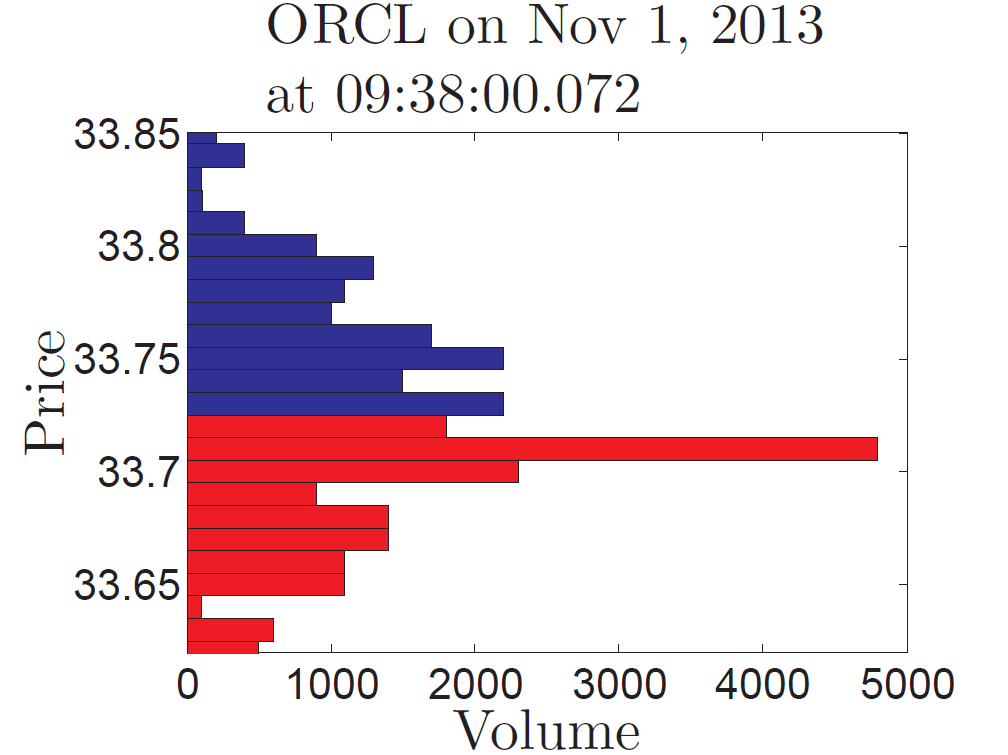
\includegraphics[scale=.60]{LOBex.PNG}
    \caption{Snapshot of the LOB Source: \parencite{cartea2015algorithmic}}
    \label{fig:1}
\end{figure}
\end{frame}

\subsection{Price Formation}

\begin{frame}
  \frametitle{\hfill Price Formation}
  Executing orders might have an impact on the remaining prices..
  \begin{columns}[t]
    \column{.4\textwidth}
    \begin{block}{Bid-ask Spread}
    \begin{itemize}
        \item Spread is the average of the bid ($b_t$) and ask ($a_t$) prices:
        \begin{equation}
            S_t = \frac{1}{2}(a_t + b_t)
        \end{equation}
        \item Spread declines over time
        \item Price Impact of trades causing $S_t$ to increase or decrease
    \end{itemize}
    \end{block}
    
    \column{.4\textwidth}
    \begin{block}{Price Impact}
    \begin{itemize}
        \item Order Imbalance:
        \begin{equation}
            I_t = \frac{V_{t}^{b}}{V_{t}^{b} + V_{t}^{a}}
        \end{equation}
        \item Price Impact Regression:
        \begin{equation}
            \Delta S_n = \lambda q_n + \varepsilon_n
        \end{equation}
        \item Lower $\lambda \rightarrow$ more liquid market, less impact
    \end{itemize}
    \end{block}
\end{columns}


\end{frame}

\subsection{Optimal Inventory}

\begin{frame}
  \frametitle{\hfill Optimal Inventory}
  \textcite{ho1981optimal} find optimal inventory levels. By optimizing the expected utility of total wealth $E[U(W_T)]$ at time horizon $T$, where 
  
\begin{equation}
    \label{eq:h2}
    J(t,F,I,Y) = \underset{a,b}{\max}[E[U(W_T)] | t,F,I,Y]
\end{equation}

It can be shown \parencite{ho1981optimal, o1995market} via stochastic optimization and dynamic programming that the optimal spread is:

\begin{equation}
    \label{eq:13h}
    s = \alpha / \beta + (J-SJ)/2SJ_{F}Q + (J-BJ)/2BJ_{F}Q
\end{equation}

\begin{itemize}
    \item The spreads depends on the time horizon of the dealer. 
    \item It can be decomposed in a risk-neutral and risky part.
    \item The spread is independent of inventory levels.
\end{itemize}

\end{frame}

%reinforcement learning
\section{Reinforcement Learning}

\begin{frame}
  \frametitle{\hfill Reinforcement Learning}
  \textit{Reinforcement Learning (RL) is learning what to do i.e. map situations to actions to maximize a numerical reward. }

  \begin{block}{}
    \begin{figure}[H]
    \centering
    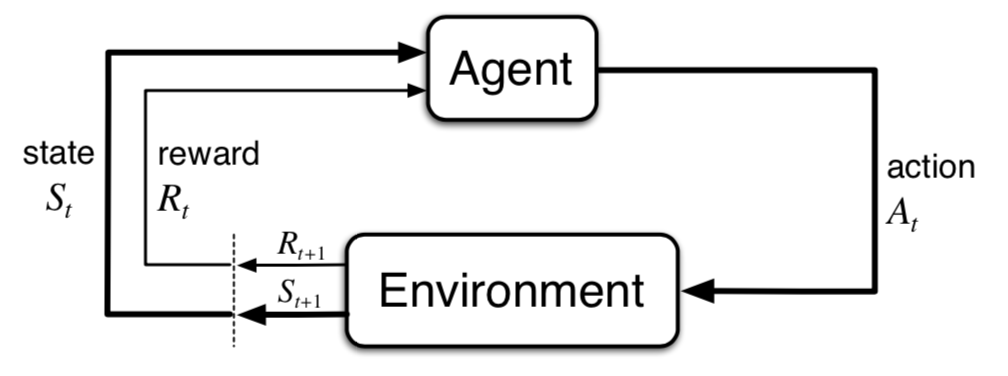
\includegraphics[scale=.60]{basicRL.png}
    \caption{Agent interacting via actions ($A_t$) with its environment moving through states ($S_t$). Thus gaining different rewards ($R_t$). Source: \textcite{sutton1998reinforcement}}
    \label{fig:2}
\end{figure}
  \end{block}

\end{frame}

\subsection{DQN \& PPO}
\begin{frame}
  \frametitle{\hfill DQN \& PPO}
  \begin{columns}[t]
    \column{.4\textwidth}
    \begin{block}{Deep Q Networks (DQN)}
    \begin{itemize}
        \item Replaces \textit{Q-function} with \textit{Q-Network}
        \item \textit{Experience Replay}
        \item Implemented in both kerasRL \& tensorforce
        \item First presented in \textcite{mnih2015human}
    \end{itemize}
    \end{block}
    
    \column{.4\textwidth}
    \begin{block}{Policy Gradients \& PPO}
    \begin{itemize}
        \item Estimate gradients of policy parameters
        \item Stochastic gradient descent \& ascent \parencite{schulman2017proximal}
        \item Also implemented in kerasRL \& tensorforce
        \item Converges more smoothly in general
    \end{itemize}
    \end{block}
\end{columns}

\end{frame}



%%%%%%%%%%%%%%%%%%%%%%%%%%%%%%%%%%%%%%%%%%%%%%%%%%%%%%%%%%%%
% Methodology
%%%%%%%%%%%%%%%%%%%%%%%%%%%%%%%%%%%%%%%%%%%%%%%%%%%%%%%%%%%%
\section{Methodology \& Implementation}

\begin{frame}
  \frametitle{\hfill Methodology}

  \begin{block}{}
    \begin{figure}[H]
    \centering
    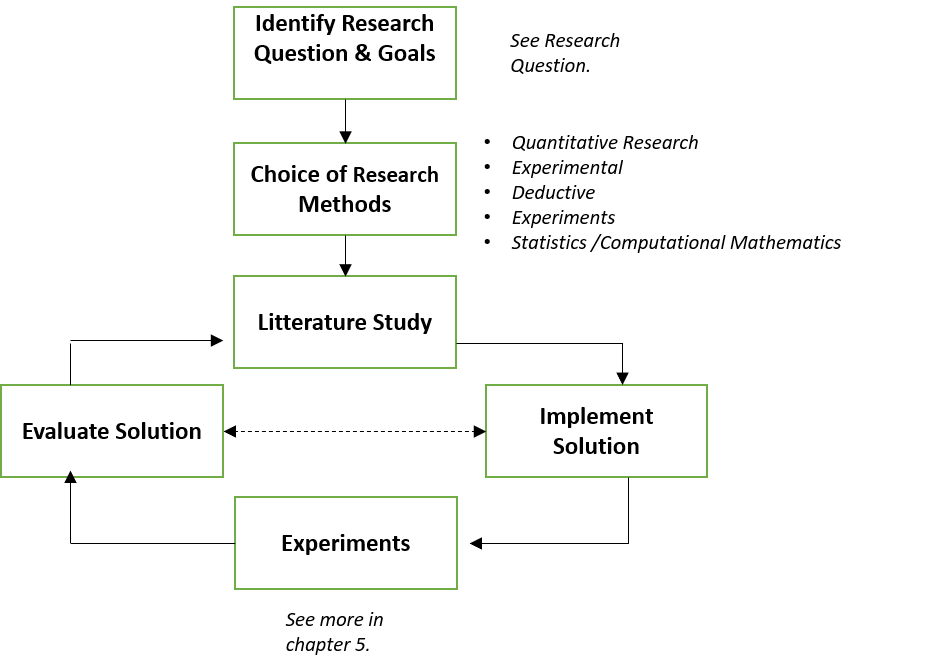
\includegraphics[scale=.50]{researchmethodsv3.PNG}
    \caption{Overview of research methodology}
    \label{fig:3}
\end{figure}
  \end{block}

\end{frame}

\begin{frame}
  \frametitle{\hfill Implementation}

  \begin{block}{}
    \begin{figure}[H]
    \centering
    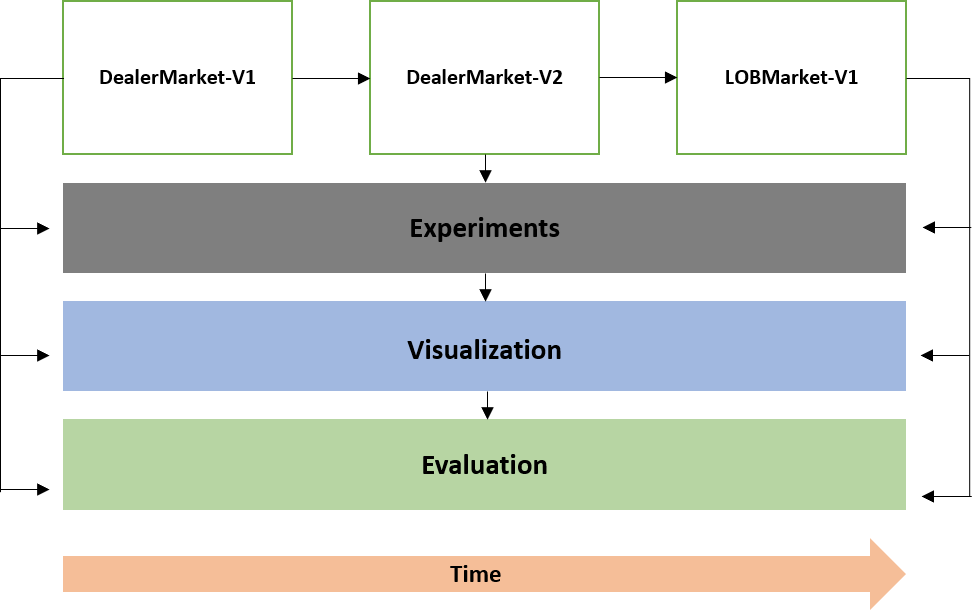
\includegraphics[scale=.55]{implementation.png}
    \caption{Overview of implementation}
    \label{fig:4}
\end{figure}
  \end{block}

\end{frame}

\begin{frame}
  \frametitle{\hfill Environments}


    \begin{table}[H]
    \centering
    \caption{Major differences between the environments.}
    \label{tab:e11}
    \resizebox{0.90\textwidth}{!}{%
        \begin{tabular}{llllllllll}
        Agent & $a_t$  & $\sigma$  & $\lambda$  & Reward  & Offset  & Slope  & $h_t$  & Funds & Inventory  \\ \hline
         dmv1 & $4$  & $0.2$  & $10$  & sparsed  & $10$  & $-$  &  $10$ & $10^6$ & $1000$ \\
         dmv2 & $6$  & $1.5$  & $5$  & sparsed & $8$  & $0.5$  & $10$  & $10^6$ & $1000$ \\
         lobv1& $10$ & $2.0$  & $150$  & shaped & $8$  & $5$  & $10$  & $2\cdot 10^5$ & $200$
        \end{tabular}%
        }
    \end{table}
    
    \begin{table}[H]
    \centering
    \caption{The different network architectures used.}
    \label{tab:e1}
    \resizebox{0.90\textwidth}{!}{%
        \begin{tabular}{llll}
         \textbf{Environment} & \textbf{Architecture}  & \textbf{Type}  & \textbf{Library}  \\ \hline
         \textit{DealerMarket-v1}& 8-layer FCNN  & DQN + Boltzmann  & keras-RL   \\
         \textit{DealerMarket-v2}& 8-layer FCNN  & PPO + $\varepsilon$ - decay  & tensorforce  \\
         %\textit{DealerMarket-V2}& ?  & PPO + Self Play  & tensorforce  \\
         \textit{DealerMarket-v2} & Random model  & Random policy  & tensorforce \\
         %\textit{LOBMarket-V1} & ?  & PPO + Self-Play  & tensorforce \\ 
         \textit{LOBMarket-v1} & 6-layer FCNN + 2 LSTM  & PPO + $\varepsilon$ - decay  & tensorforce \\ 
         \textit{LOBMarket-v1} & Random model  & Random policy  & tensorforce
        \end{tabular}%
        }
    \end{table}
     

\end{frame}

\begin{frame}
  \frametitle{\hfill Network Architecture}

  \begin{block}{}
    \begin{figure}[H]
    \centering
    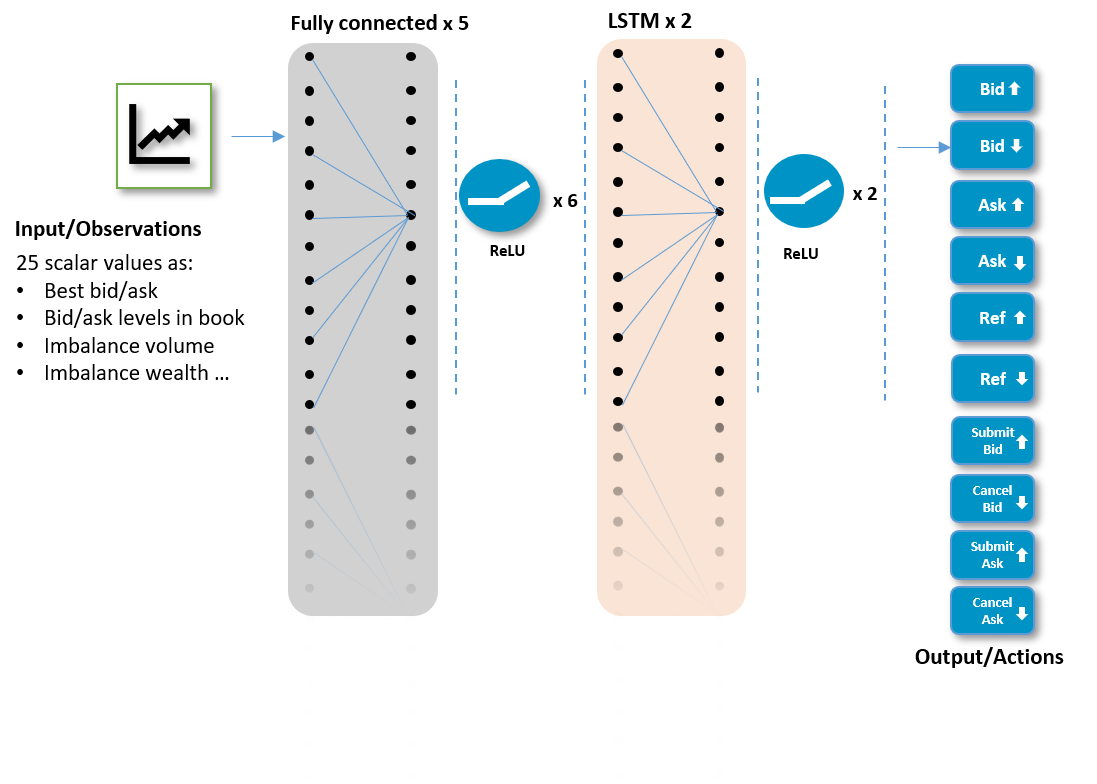
\includegraphics[scale=.40]{nnalob1.png}
    \caption{Network architecture for LOB agent}
    \label{fig:5}
\end{figure}
  \end{block}

\end{frame}


%%%%%%%%%%%%%%%%%%%%%%%%%%%%%%%%%%%%%%%%%%%%%%%%%%%%%%%%%%%%
% Results
%%%%%%%%%%%%%%%%%%%%%%%%%%%%%%%%%%%%%%%%%%%%%%%%%%%%%%%%%%%%

\section{Results}

\begin{frame}
  \frametitle{\hfill Results}
  \begin{table}[H]
    \centering
    \caption{Table over rewards for DealerMarket-v1, DealerMarket-v2 and LOBMarket-v1.}
    \label{tab:dm1}
    \begin{tabular}{rrrrrr}
      \hline
     \textbf{Model} & \textbf{Mean} & \textbf{Std} & \textbf{Max} & \textbf{Min} & \textbf{CI} \\ 
      \hline
    DealerMarket-v1 & $391.88$ & $150.47$ & $478.04$ & $-9.43$ & $16.18$ \\
    DealerMarket-v2 & $22.47$ & $78.46$ & $347.40$ & $-816.11$ & $2.85$  \\
    LOBMarket-v1& $-5.02$ & $23.88$ & $145.46$ & $-526.77$ & $0.88$ \\ 
    
       \hline
\end{tabular}
\end{table}

\begin{table}[H]
    \centering
    \caption{Table over P\&L for DealerMarket-v2 and LOBMarket-v1.}
    \label{tab:pnl1}
    \resizebox{0.95\textwidth}{!}{%
    \begin{tabular}{rrrrrr}
      \hline
     \textbf{Model} & \textbf{Mean} & \textbf{Std} & \textbf{Max} & \textbf{Min} & \textbf{CI} \\ 
      \hline
    DealerMarket-v2 & $-18861.06$ & $540266.01$ & $2220487.97$ & $-1436406.28$ & $19650.46$ \\ 
    LOBMarket-v1& $-3366.20$ & $60769.67$ & $313634.96$ & $-334806.89$ & $2236.15$ \\ 
       \hline
    \end{tabular}%
}
\end{table}
  
\end{frame}

\subsection{Stylized Facts}

\begin{frame}
  \frametitle{\hfill Stylized Facts}
  \begin{figure}[H]
		%Do not try to scale figure in .tex or you loose font size consistency
		\centering
		%The code to input the plot is extremely simple
		%% Created by tikzDevice version 0.11 on 2018-07-15 13:37:11
% !TEX encoding = UTF-8 Unicode
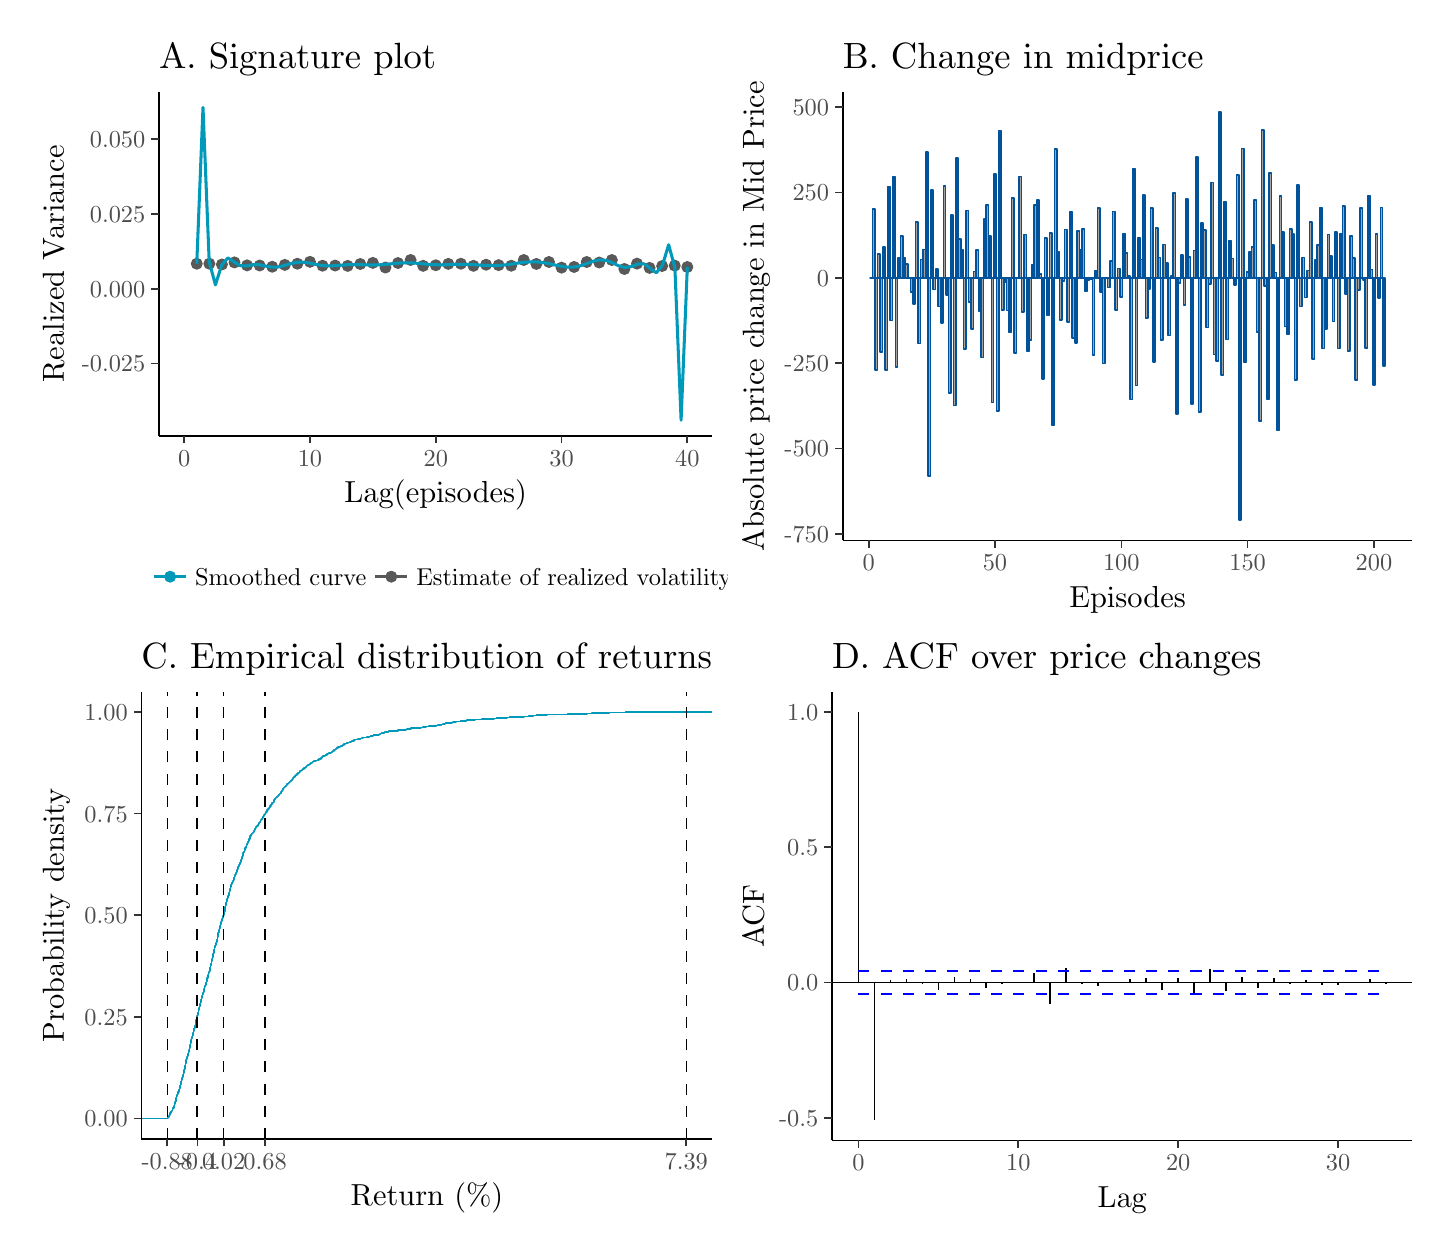
\begin{tikzpicture}[x=1pt,y=1pt]
\definecolor{fillColor}{RGB}{255,255,255}
\path[use as bounding box,fill=fillColor,fill opacity=0.00] (0,0) rectangle (505.89,433.62);
\begin{scope}
\path[clip] (  0.00,216.81) rectangle (252.95,433.62);
\definecolor{drawColor}{RGB}{255,255,255}
\definecolor{fillColor}{RGB}{255,255,255}

\path[draw=drawColor,line width= 0.6pt,line join=round,line cap=round,fill=fillColor] ( -0.00,216.81) rectangle (252.95,433.62);
\end{scope}
\begin{scope}
\path[clip] ( 47.47,286.11) rectangle (247.44,410.48);
\definecolor{fillColor}{RGB}{255,255,255}

\path[fill=fillColor] ( 47.47,286.11) rectangle (247.44,410.48);
\definecolor{drawColor}{gray}{0.35}
\definecolor{fillColor}{gray}{0.35}

\path[draw=drawColor,line width= 0.4pt,line join=round,line cap=round,fill=fillColor] ( 61.10,348.32) circle (  1.96);

\path[draw=drawColor,line width= 0.4pt,line join=round,line cap=round,fill=fillColor] ( 65.65,348.33) circle (  1.96);

\path[draw=drawColor,line width= 0.4pt,line join=round,line cap=round,fill=fillColor] ( 70.19,348.05) circle (  1.96);

\path[draw=drawColor,line width= 0.4pt,line join=round,line cap=round,fill=fillColor] ( 74.74,348.79) circle (  1.96);

\path[draw=drawColor,line width= 0.4pt,line join=round,line cap=round,fill=fillColor] ( 79.28,347.72) circle (  1.96);

\path[draw=drawColor,line width= 0.4pt,line join=round,line cap=round,fill=fillColor] ( 83.83,347.68) circle (  1.96);

\path[draw=drawColor,line width= 0.4pt,line join=round,line cap=round,fill=fillColor] ( 88.37,347.23) circle (  1.96);

\path[draw=drawColor,line width= 0.4pt,line join=round,line cap=round,fill=fillColor] ( 92.92,347.90) circle (  1.96);

\path[draw=drawColor,line width= 0.4pt,line join=round,line cap=round,fill=fillColor] ( 97.46,348.32) circle (  1.96);

\path[draw=drawColor,line width= 0.4pt,line join=round,line cap=round,fill=fillColor] (102.01,349.00) circle (  1.96);

\path[draw=drawColor,line width= 0.4pt,line join=round,line cap=round,fill=fillColor] (106.55,347.60) circle (  1.96);

\path[draw=drawColor,line width= 0.4pt,line join=round,line cap=round,fill=fillColor] (111.10,347.66) circle (  1.96);

\path[draw=drawColor,line width= 0.4pt,line join=round,line cap=round,fill=fillColor] (115.64,347.54) circle (  1.96);

\path[draw=drawColor,line width= 0.4pt,line join=round,line cap=round,fill=fillColor] (120.19,348.22) circle (  1.96);

\path[draw=drawColor,line width= 0.4pt,line join=round,line cap=round,fill=fillColor] (124.73,348.62) circle (  1.96);

\path[draw=drawColor,line width= 0.4pt,line join=round,line cap=round,fill=fillColor] (129.28,346.94) circle (  1.96);

\path[draw=drawColor,line width= 0.4pt,line join=round,line cap=round,fill=fillColor] (133.82,348.57) circle (  1.96);

\path[draw=drawColor,line width= 0.4pt,line join=round,line cap=round,fill=fillColor] (138.37,349.67) circle (  1.96);

\path[draw=drawColor,line width= 0.4pt,line join=round,line cap=round,fill=fillColor] (142.91,347.56) circle (  1.96);

\path[draw=drawColor,line width= 0.4pt,line join=round,line cap=round,fill=fillColor] (147.46,347.77) circle (  1.96);

\path[draw=drawColor,line width= 0.4pt,line join=round,line cap=round,fill=fillColor] (152.00,348.26) circle (  1.96);

\path[draw=drawColor,line width= 0.4pt,line join=round,line cap=round,fill=fillColor] (156.55,348.31) circle (  1.96);

\path[draw=drawColor,line width= 0.4pt,line join=round,line cap=round,fill=fillColor] (161.09,347.56) circle (  1.96);

\path[draw=drawColor,line width= 0.4pt,line join=round,line cap=round,fill=fillColor] (165.64,347.96) circle (  1.96);

\path[draw=drawColor,line width= 0.4pt,line join=round,line cap=round,fill=fillColor] (170.18,347.81) circle (  1.96);

\path[draw=drawColor,line width= 0.4pt,line join=round,line cap=round,fill=fillColor] (174.73,347.60) circle (  1.96);

\path[draw=drawColor,line width= 0.4pt,line join=round,line cap=round,fill=fillColor] (179.27,349.66) circle (  1.96);

\path[draw=drawColor,line width= 0.4pt,line join=round,line cap=round,fill=fillColor] (183.82,348.24) circle (  1.96);

\path[draw=drawColor,line width= 0.4pt,line join=round,line cap=round,fill=fillColor] (188.36,348.95) circle (  1.96);

\path[draw=drawColor,line width= 0.4pt,line join=round,line cap=round,fill=fillColor] (192.91,346.91) circle (  1.96);

\path[draw=drawColor,line width= 0.4pt,line join=round,line cap=round,fill=fillColor] (197.45,347.15) circle (  1.96);

\path[draw=drawColor,line width= 0.4pt,line join=round,line cap=round,fill=fillColor] (202.00,348.94) circle (  1.96);

\path[draw=drawColor,line width= 0.4pt,line join=round,line cap=round,fill=fillColor] (206.54,348.75) circle (  1.96);

\path[draw=drawColor,line width= 0.4pt,line join=round,line cap=round,fill=fillColor] (211.09,349.66) circle (  1.96);

\path[draw=drawColor,line width= 0.4pt,line join=round,line cap=round,fill=fillColor] (215.63,346.42) circle (  1.96);

\path[draw=drawColor,line width= 0.4pt,line join=round,line cap=round,fill=fillColor] (220.18,348.35) circle (  1.96);

\path[draw=drawColor,line width= 0.4pt,line join=round,line cap=round,fill=fillColor] (224.72,346.81) circle (  1.96);

\path[draw=drawColor,line width= 0.4pt,line join=round,line cap=round,fill=fillColor] (229.27,347.49) circle (  1.96);

\path[draw=drawColor,line width= 0.4pt,line join=round,line cap=round,fill=fillColor] (233.81,347.63) circle (  1.96);

\path[draw=drawColor,line width= 0.4pt,line join=round,line cap=round,fill=fillColor] (238.36,347.13) circle (  1.96);
\definecolor{drawColor}{RGB}{0,153,186}

\path[draw=drawColor,line width= 1.1pt,line join=round] ( 61.10,348.32) --
	( 63.35,404.83) --
	( 65.59,349.07) --
	( 67.84,340.67) --
	( 70.08,347.74) --
	( 72.32,350.41) --
	( 74.57,348.99) --
	( 76.81,347.60) --
	( 79.05,347.54) --
	( 81.30,347.95) --
	( 83.54,347.96) --
	( 85.79,347.51) --
	( 88.03,347.08) --
	( 90.27,347.10) --
	( 92.52,347.61) --
	( 94.76,348.30) --
	( 97.00,348.80) --
	( 99.25,348.90) --
	(101.49,348.62) --
	(103.73,348.16) --
	(105.98,347.75) --
	(108.22,347.55) --
	(110.47,347.58) --
	(112.71,347.75) --
	(114.95,347.93) --
	(117.20,348.02) --
	(119.44,348.00) --
	(121.68,347.92) --
	(123.93,347.85) --
	(126.17,347.87) --
	(128.42,348.01) --
	(130.66,348.22) --
	(132.90,348.45) --
	(135.15,348.61) --
	(137.39,348.65) --
	(139.63,348.56) --
	(141.88,348.37) --
	(144.12,348.16) --
	(146.36,348.00) --
	(148.61,347.93) --
	(150.85,347.94) --
	(153.10,348.02) --
	(155.34,348.09) --
	(157.58,348.11) --
	(159.83,348.05) --
	(162.07,347.92) --
	(164.31,347.77) --
	(166.56,347.66) --
	(168.80,347.64) --
	(171.04,347.75) --
	(173.29,347.99) --
	(175.53,348.30) --
	(177.78,348.64) --
	(180.02,348.90) --
	(182.26,349.01) --
	(184.51,348.94) --
	(186.75,348.66) --
	(188.99,348.21) --
	(191.24,347.70) --
	(193.48,347.26) --
	(195.73,347.04) --
	(197.97,347.18) --
	(200.21,347.72) --
	(202.46,348.54) --
	(204.70,349.33) --
	(206.94,349.74) --
	(209.19,349.49) --
	(211.43,348.60) --
	(213.67,347.52) --
	(215.92,346.95) --
	(218.16,347.31) --
	(220.41,348.20) --
	(222.65,348.31) --
	(224.89,346.71) --
	(227.14,345.02) --
	(229.38,347.79) --
	(231.62,355.19) --
	(233.87,346.89) --
	(236.11,291.77) --
	(238.36,347.13);
\end{scope}
\begin{scope}
\path[clip] (  0.00,  0.00) rectangle (505.89,433.62);
\definecolor{drawColor}{RGB}{0,0,0}

\path[draw=drawColor,line width= 0.6pt,line join=round] ( 47.47,286.11) --
	( 47.47,410.48);
\end{scope}
\begin{scope}
\path[clip] (  0.00,  0.00) rectangle (505.89,433.62);
\definecolor{drawColor}{gray}{0.30}

\node[text=drawColor,anchor=base east,inner sep=0pt, outer sep=0pt, scale=  0.88] at ( 42.52,309.20) {-0.025};

\node[text=drawColor,anchor=base east,inner sep=0pt, outer sep=0pt, scale=  0.88] at ( 42.52,336.24) {0.000};

\node[text=drawColor,anchor=base east,inner sep=0pt, outer sep=0pt, scale=  0.88] at ( 42.52,363.28) {0.025};

\node[text=drawColor,anchor=base east,inner sep=0pt, outer sep=0pt, scale=  0.88] at ( 42.52,390.31) {0.050};
\end{scope}
\begin{scope}
\path[clip] (  0.00,  0.00) rectangle (505.89,433.62);
\definecolor{drawColor}{gray}{0.20}

\path[draw=drawColor,line width= 0.6pt,line join=round] ( 44.72,312.23) --
	( 47.47,312.23);

\path[draw=drawColor,line width= 0.6pt,line join=round] ( 44.72,339.27) --
	( 47.47,339.27);

\path[draw=drawColor,line width= 0.6pt,line join=round] ( 44.72,366.31) --
	( 47.47,366.31);

\path[draw=drawColor,line width= 0.6pt,line join=round] ( 44.72,393.34) --
	( 47.47,393.34);
\end{scope}
\begin{scope}
\path[clip] (  0.00,  0.00) rectangle (505.89,433.62);
\definecolor{drawColor}{RGB}{0,0,0}

\path[draw=drawColor,line width= 0.6pt,line join=round] ( 47.47,286.11) --
	(247.44,286.11);
\end{scope}
\begin{scope}
\path[clip] (  0.00,  0.00) rectangle (505.89,433.62);
\definecolor{drawColor}{gray}{0.20}

\path[draw=drawColor,line width= 0.6pt,line join=round] ( 56.56,283.36) --
	( 56.56,286.11);

\path[draw=drawColor,line width= 0.6pt,line join=round] (102.01,283.36) --
	(102.01,286.11);

\path[draw=drawColor,line width= 0.6pt,line join=round] (147.46,283.36) --
	(147.46,286.11);

\path[draw=drawColor,line width= 0.6pt,line join=round] (192.91,283.36) --
	(192.91,286.11);

\path[draw=drawColor,line width= 0.6pt,line join=round] (238.36,283.36) --
	(238.36,286.11);
\end{scope}
\begin{scope}
\path[clip] (  0.00,  0.00) rectangle (505.89,433.62);
\definecolor{drawColor}{gray}{0.30}

\node[text=drawColor,anchor=base,inner sep=0pt, outer sep=0pt, scale=  0.88] at ( 56.56,275.10) {0};

\node[text=drawColor,anchor=base,inner sep=0pt, outer sep=0pt, scale=  0.88] at (102.01,275.10) {10};

\node[text=drawColor,anchor=base,inner sep=0pt, outer sep=0pt, scale=  0.88] at (147.46,275.10) {20};

\node[text=drawColor,anchor=base,inner sep=0pt, outer sep=0pt, scale=  0.88] at (192.91,275.10) {30};

\node[text=drawColor,anchor=base,inner sep=0pt, outer sep=0pt, scale=  0.88] at (238.36,275.10) {40};
\end{scope}
\begin{scope}
\path[clip] (  0.00,  0.00) rectangle (505.89,433.62);
\definecolor{drawColor}{RGB}{0,0,0}

\node[text=drawColor,anchor=base,inner sep=0pt, outer sep=0pt, scale=  1.10] at (147.46,262.03) {Lag(episodes)};
\end{scope}
\begin{scope}
\path[clip] (  0.00,  0.00) rectangle (505.89,433.62);
\definecolor{drawColor}{RGB}{0,0,0}

\node[text=drawColor,rotate= 90.00,anchor=base,inner sep=0pt, outer sep=0pt, scale=  1.10] at ( 13.08,348.30) {Realized Variance};
\end{scope}
\begin{scope}
\path[clip] (  0.00,  0.00) rectangle (505.89,433.62);
\definecolor{fillColor}{RGB}{255,255,255}

\path[fill=fillColor] ( 34.95,222.31) rectangle (259.96,248.15);
\end{scope}
\begin{scope}
\path[clip] (  0.00,  0.00) rectangle (505.89,433.62);
\definecolor{drawColor}{RGB}{0,153,186}
\definecolor{fillColor}{RGB}{0,153,186}

\path[draw=drawColor,line width= 0.4pt,line join=round,line cap=round,fill=fillColor] ( 51.48,235.23) circle (  1.96);
\end{scope}
\begin{scope}
\path[clip] (  0.00,  0.00) rectangle (505.89,433.62);
\definecolor{drawColor}{RGB}{0,153,186}

\path[draw=drawColor,line width= 1.1pt,line join=round] ( 45.70,235.23) -- ( 57.26,235.23);
\end{scope}
\begin{scope}
\path[clip] (  0.00,  0.00) rectangle (505.89,433.62);
\definecolor{drawColor}{gray}{0.35}
\definecolor{fillColor}{gray}{0.35}

\path[draw=drawColor,line width= 0.4pt,line join=round,line cap=round,fill=fillColor] (131.40,235.23) circle (  1.96);
\end{scope}
\begin{scope}
\path[clip] (  0.00,  0.00) rectangle (505.89,433.62);
\definecolor{drawColor}{gray}{0.35}

\path[draw=drawColor,line width= 1.1pt,line join=round] (125.62,235.23) -- (137.19,235.23);
\end{scope}
\begin{scope}
\path[clip] (  0.00,  0.00) rectangle (505.89,433.62);
\definecolor{drawColor}{RGB}{0,0,0}

\node[text=drawColor,anchor=base west,inner sep=0pt, outer sep=0pt, scale=  0.88] at ( 60.52,232.20) {Smoothed curve};
\end{scope}
\begin{scope}
\path[clip] (  0.00,  0.00) rectangle (505.89,433.62);
\definecolor{drawColor}{RGB}{0,0,0}

\node[text=drawColor,anchor=base west,inner sep=0pt, outer sep=0pt, scale=  0.88] at (140.44,232.20) {Estimate of realized volatility};
\end{scope}
\begin{scope}
\path[clip] (  0.00,  0.00) rectangle (505.89,433.62);
\definecolor{drawColor}{RGB}{0,0,0}

\node[text=drawColor,anchor=base west,inner sep=0pt, outer sep=0pt, scale=  1.32] at ( 47.47,419.03) {A. Signature plot};
\end{scope}
\begin{scope}
\path[clip] (  0.00,  0.00) rectangle (252.94,216.81);
\definecolor{drawColor}{RGB}{255,255,255}
\definecolor{fillColor}{RGB}{255,255,255}

\path[draw=drawColor,line width= 0.6pt,line join=round,line cap=round,fill=fillColor] (  0.00,  0.00) rectangle (252.94,216.81);
\end{scope}
\begin{scope}
\path[clip] ( 41.11, 32.09) rectangle (247.44,193.67);
\definecolor{fillColor}{RGB}{255,255,255}

\path[fill=fillColor] ( 41.11, 32.09) rectangle (247.44,193.67);
\definecolor{drawColor}{RGB}{0,153,186}

\path[draw=drawColor,line width= 0.6pt,line join=round] ( 41.11, 39.43) --
	( 50.49, 39.43) --
	( 50.49, 39.50) --
	( 50.56, 39.50) --
	( 50.56, 39.57) --
	( 50.72, 39.57) --
	( 50.72, 39.65) --
	( 50.76, 39.65) --
	( 50.76, 39.72) --
	( 50.76, 39.72) --
	( 50.76, 39.79) --
	( 50.78, 39.79) --
	( 50.78, 39.86) --
	( 50.84, 39.86) --
	( 50.84, 39.93) --
	( 50.91, 39.93) --
	( 50.91, 40.01) --
	( 50.94, 40.01) --
	( 50.94, 40.08) --
	( 51.03, 40.08) --
	( 51.03, 40.15) --
	( 51.03, 40.15) --
	( 51.03, 40.22) --
	( 51.07, 40.22) --
	( 51.07, 40.29) --
	( 51.08, 40.29) --
	( 51.08, 40.36) --
	( 51.09, 40.36) --
	( 51.09, 40.44) --
	( 51.12, 40.44) --
	( 51.12, 40.51) --
	( 51.17, 40.51) --
	( 51.17, 40.58) --
	( 51.21, 40.58) --
	( 51.21, 40.65) --
	( 51.31, 40.65) --
	( 51.31, 40.72) --
	( 51.34, 40.72) --
	( 51.34, 40.79) --
	( 51.35, 40.79) --
	( 51.35, 40.87) --
	( 51.38, 40.87) --
	( 51.38, 40.94) --
	( 51.38, 40.94) --
	( 51.38, 41.01) --
	( 51.39, 41.01) --
	( 51.39, 41.08) --
	( 51.40, 41.08) --
	( 51.40, 41.15) --
	( 51.41, 41.15) --
	( 51.41, 41.23) --
	( 51.49, 41.23) --
	( 51.49, 41.30) --
	( 51.51, 41.30) --
	( 51.51, 41.37) --
	( 51.63, 41.37) --
	( 51.63, 41.44) --
	( 51.69, 41.44) --
	( 51.69, 41.51) --
	( 51.71, 41.51) --
	( 51.71, 41.58) --
	( 51.71, 41.58) --
	( 51.71, 41.66) --
	( 51.72, 41.66) --
	( 51.72, 41.73) --
	( 51.75, 41.73) --
	( 51.75, 41.80) --
	( 51.79, 41.80) --
	( 51.79, 41.87) --
	( 51.83, 41.87) --
	( 51.83, 41.94) --
	( 51.88, 41.94) --
	( 51.88, 42.01) --
	( 51.92, 42.01) --
	( 51.92, 42.09) --
	( 51.96, 42.09) --
	( 51.96, 42.16) --
	( 52.20, 42.16) --
	( 52.20, 42.23) --
	( 52.20, 42.23) --
	( 52.20, 42.30) --
	( 52.22, 42.30) --
	( 52.22, 42.37) --
	( 52.28, 42.37) --
	( 52.28, 42.45) --
	( 52.29, 42.45) --
	( 52.29, 42.52) --
	( 52.29, 42.52) --
	( 52.29, 42.59) --
	( 52.29, 42.59) --
	( 52.29, 42.66) --
	( 52.33, 42.66) --
	( 52.33, 42.73) --
	( 52.39, 42.73) --
	( 52.39, 42.80) --
	( 52.46, 42.80) --
	( 52.46, 42.88) --
	( 52.50, 42.88) --
	( 52.50, 42.95) --
	( 52.50, 42.95) --
	( 52.50, 43.02) --
	( 52.57, 43.02) --
	( 52.57, 43.09) --
	( 52.62, 43.09) --
	( 52.62, 43.16) --
	( 52.65, 43.16) --
	( 52.65, 43.23) --
	( 52.74, 43.23) --
	( 52.74, 43.31) --
	( 52.77, 43.31) --
	( 52.77, 43.38) --
	( 52.80, 43.38) --
	( 52.80, 43.45) --
	( 52.83, 43.45) --
	( 52.83, 43.52) --
	( 52.85, 43.52) --
	( 52.85, 43.59) --
	( 52.85, 43.59) --
	( 52.85, 43.67) --
	( 52.87, 43.67) --
	( 52.87, 43.74) --
	( 52.99, 43.74) --
	( 52.99, 43.81) --
	( 52.99, 43.81) --
	( 52.99, 43.88) --
	( 53.00, 43.88) --
	( 53.00, 43.95) --
	( 53.03, 43.95) --
	( 53.03, 44.02) --
	( 53.03, 44.02) --
	( 53.03, 44.10) --
	( 53.05, 44.10) --
	( 53.05, 44.17) --
	( 53.07, 44.17) --
	( 53.07, 44.24) --
	( 53.09, 44.24) --
	( 53.09, 44.31) --
	( 53.10, 44.31) --
	( 53.10, 44.38) --
	( 53.10, 44.38) --
	( 53.10, 44.45) --
	( 53.10, 44.45) --
	( 53.10, 44.53) --
	( 53.10, 44.53) --
	( 53.10, 44.60) --
	( 53.11, 44.60) --
	( 53.11, 44.67) --
	( 53.11, 44.67) --
	( 53.11, 44.74) --
	( 53.13, 44.74) --
	( 53.13, 44.81) --
	( 53.18, 44.81) --
	( 53.18, 44.89) --
	( 53.20, 44.89) --
	( 53.20, 44.96) --
	( 53.26, 44.96) --
	( 53.26, 45.03) --
	( 53.27, 45.03) --
	( 53.27, 45.10) --
	( 53.28, 45.10) --
	( 53.28, 45.17) --
	( 53.28, 45.17) --
	( 53.28, 45.24) --
	( 53.30, 45.24) --
	( 53.30, 45.32) --
	( 53.31, 45.32) --
	( 53.31, 45.39) --
	( 53.32, 45.39) --
	( 53.32, 45.46) --
	( 53.36, 45.46) --
	( 53.36, 45.53) --
	( 53.40, 45.53) --
	( 53.40, 45.60) --
	( 53.48, 45.60) --
	( 53.48, 45.67) --
	( 53.49, 45.67) --
	( 53.49, 45.75) --
	( 53.49, 45.75) --
	( 53.49, 45.82) --
	( 53.52, 45.82) --
	( 53.52, 45.89) --
	( 53.53, 45.89) --
	( 53.53, 45.96) --
	( 53.55, 45.96) --
	( 53.55, 46.03) --
	( 53.56, 46.03) --
	( 53.56, 46.11) --
	( 53.57, 46.11) --
	( 53.57, 46.18) --
	( 53.57, 46.18) --
	( 53.57, 46.25) --
	( 53.59, 46.25) --
	( 53.59, 46.32) --
	( 53.60, 46.32) --
	( 53.60, 46.39) --
	( 53.63, 46.39) --
	( 53.63, 46.46) --
	( 53.65, 46.46) --
	( 53.65, 46.54) --
	( 53.66, 46.54) --
	( 53.66, 46.61) --
	( 53.66, 46.61) --
	( 53.66, 46.68) --
	( 53.67, 46.68) --
	( 53.67, 46.75) --
	( 53.69, 46.75) --
	( 53.69, 46.82) --
	( 53.69, 46.82) --
	( 53.69, 46.89) --
	( 53.69, 46.89) --
	( 53.69, 46.97) --
	( 53.72, 46.97) --
	( 53.72, 47.04) --
	( 53.73, 47.04) --
	( 53.73, 47.11) --
	( 53.74, 47.11) --
	( 53.74, 47.18) --
	( 53.76, 47.18) --
	( 53.76, 47.25) --
	( 53.77, 47.25) --
	( 53.77, 47.33) --
	( 53.82, 47.33) --
	( 53.82, 47.40) --
	( 53.85, 47.40) --
	( 53.85, 47.47) --
	( 53.90, 47.47) --
	( 53.90, 47.54) --
	( 53.94, 47.54) --
	( 53.94, 47.61) --
	( 53.94, 47.61) --
	( 53.94, 47.68) --
	( 54.01, 47.68) --
	( 54.01, 47.76) --
	( 54.01, 47.76) --
	( 54.01, 47.83) --
	( 54.07, 47.83) --
	( 54.07, 47.90) --
	( 54.09, 47.90) --
	( 54.09, 47.97) --
	( 54.16, 47.97) --
	( 54.16, 48.04) --
	( 54.17, 48.04) --
	( 54.17, 48.11) --
	( 54.17, 48.11) --
	( 54.17, 48.19) --
	( 54.20, 48.19) --
	( 54.20, 48.26) --
	( 54.21, 48.26) --
	( 54.21, 48.33) --
	( 54.28, 48.33) --
	( 54.28, 48.40) --
	( 54.28, 48.40) --
	( 54.28, 48.47) --
	( 54.30, 48.47) --
	( 54.30, 48.54) --
	( 54.35, 48.54) --
	( 54.35, 48.62) --
	( 54.36, 48.62) --
	( 54.36, 48.69) --
	( 54.37, 48.69) --
	( 54.37, 48.76) --
	( 54.37, 48.76) --
	( 54.37, 48.83) --
	( 54.42, 48.83) --
	( 54.42, 48.90) --
	( 54.43, 48.90) --
	( 54.43, 48.98) --
	( 54.43, 48.98) --
	( 54.43, 49.05) --
	( 54.44, 49.05) --
	( 54.44, 49.12) --
	( 54.57, 49.12) --
	( 54.57, 49.19) --
	( 54.59, 49.19) --
	( 54.59, 49.26) --
	( 54.61, 49.26) --
	( 54.61, 49.33) --
	( 54.61, 49.33) --
	( 54.61, 49.41) --
	( 54.61, 49.41) --
	( 54.61, 49.48) --
	( 54.72, 49.48) --
	( 54.72, 49.55) --
	( 54.73, 49.55) --
	( 54.73, 49.62) --
	( 54.73, 49.62) --
	( 54.73, 49.69) --
	( 54.74, 49.69) --
	( 54.74, 49.76) --
	( 54.78, 49.76) --
	( 54.78, 49.84) --
	( 54.79, 49.84) --
	( 54.79, 49.91) --
	( 54.80, 49.91) --
	( 54.80, 49.98) --
	( 54.82, 49.98) --
	( 54.82, 50.05) --
	( 54.87, 50.05) --
	( 54.87, 50.12) --
	( 54.90, 50.12) --
	( 54.90, 50.20) --
	( 54.91, 50.20) --
	( 54.91, 50.27) --
	( 54.93, 50.27) --
	( 54.93, 50.34) --
	( 54.94, 50.34) --
	( 54.94, 50.41) --
	( 54.94, 50.41) --
	( 54.94, 50.48) --
	( 54.97, 50.48) --
	( 54.97, 50.55) --
	( 55.00, 50.55) --
	( 55.00, 50.63) --
	( 55.03, 50.63) --
	( 55.03, 50.70) --
	( 55.05, 50.70) --
	( 55.05, 50.77) --
	( 55.08, 50.77) --
	( 55.08, 50.84) --
	( 55.09, 50.84) --
	( 55.09, 50.91) --
	( 55.09, 50.91) --
	( 55.09, 50.98) --
	( 55.11, 50.98) --
	( 55.11, 51.06) --
	( 55.12, 51.06) --
	( 55.12, 51.13) --
	( 55.12, 51.13) --
	( 55.12, 51.20) --
	( 55.14, 51.20) --
	( 55.14, 51.27) --
	( 55.14, 51.27) --
	( 55.14, 51.34) --
	( 55.16, 51.34) --
	( 55.16, 51.42) --
	( 55.19, 51.42) --
	( 55.19, 51.49) --
	( 55.20, 51.49) --
	( 55.20, 51.56) --
	( 55.21, 51.56) --
	( 55.21, 51.63) --
	( 55.21, 51.63) --
	( 55.21, 51.70) --
	( 55.28, 51.70) --
	( 55.28, 51.77) --
	( 55.30, 51.77) --
	( 55.30, 51.85) --
	( 55.31, 51.85) --
	( 55.31, 51.92) --
	( 55.31, 51.92) --
	( 55.31, 51.99) --
	( 55.34, 51.99) --
	( 55.34, 52.06) --
	( 55.35, 52.06) --
	( 55.35, 52.13) --
	( 55.37, 52.13) --
	( 55.37, 52.20) --
	( 55.41, 52.20) --
	( 55.41, 52.28) --
	( 55.42, 52.28) --
	( 55.42, 52.35) --
	( 55.42, 52.35) --
	( 55.42, 52.42) --
	( 55.43, 52.42) --
	( 55.43, 52.49) --
	( 55.43, 52.49) --
	( 55.43, 52.56) --
	( 55.47, 52.56) --
	( 55.47, 52.64) --
	( 55.48, 52.64) --
	( 55.48, 52.71) --
	( 55.52, 52.71) --
	( 55.52, 52.78) --
	( 55.54, 52.78) --
	( 55.54, 52.85) --
	( 55.54, 52.85) --
	( 55.54, 52.92) --
	( 55.57, 52.92) --
	( 55.57, 52.99) --
	( 55.57, 52.99) --
	( 55.57, 53.07) --
	( 55.60, 53.07) --
	( 55.60, 53.14) --
	( 55.60, 53.14) --
	( 55.60, 53.21) --
	( 55.62, 53.21) --
	( 55.62, 53.28) --
	( 55.67, 53.28) --
	( 55.67, 53.35) --
	( 55.71, 53.35) --
	( 55.71, 53.42) --
	( 55.75, 53.42) --
	( 55.75, 53.50) --
	( 55.76, 53.50) --
	( 55.76, 53.57) --
	( 55.76, 53.57) --
	( 55.76, 53.64) --
	( 55.81, 53.64) --
	( 55.81, 53.71) --
	( 55.84, 53.71) --
	( 55.84, 53.78) --
	( 55.84, 53.78) --
	( 55.84, 53.86) --
	( 55.86, 53.86) --
	( 55.86, 53.93) --
	( 55.87, 53.93) --
	( 55.87, 54.00) --
	( 55.88, 54.00) --
	( 55.88, 54.07) --
	( 55.89, 54.07) --
	( 55.89, 54.14) --
	( 55.89, 54.14) --
	( 55.89, 54.21) --
	( 55.92, 54.21) --
	( 55.92, 54.29) --
	( 55.99, 54.29) --
	( 55.99, 54.36) --
	( 56.00, 54.36) --
	( 56.00, 54.43) --
	( 56.10, 54.43) --
	( 56.10, 54.50) --
	( 56.12, 54.50) --
	( 56.12, 54.57) --
	( 56.12, 54.57) --
	( 56.12, 54.64) --
	( 56.16, 54.64) --
	( 56.16, 54.72) --
	( 56.18, 54.72) --
	( 56.18, 54.79) --
	( 56.19, 54.79) --
	( 56.19, 54.86) --
	( 56.20, 54.86) --
	( 56.20, 54.93) --
	( 56.20, 54.93) --
	( 56.20, 55.00) --
	( 56.21, 55.00) --
	( 56.21, 55.08) --
	( 56.24, 55.08) --
	( 56.24, 55.15) --
	( 56.25, 55.15) --
	( 56.25, 55.22) --
	( 56.26, 55.22) --
	( 56.26, 55.29) --
	( 56.26, 55.29) --
	( 56.26, 55.36) --
	( 56.28, 55.36) --
	( 56.28, 55.43) --
	( 56.29, 55.43) --
	( 56.29, 55.51) --
	( 56.33, 55.51) --
	( 56.33, 55.58) --
	( 56.34, 55.58) --
	( 56.34, 55.65) --
	( 56.34, 55.65) --
	( 56.34, 55.72) --
	( 56.36, 55.72) --
	( 56.36, 55.79) --
	( 56.38, 55.79) --
	( 56.38, 55.86) --
	( 56.39, 55.86) --
	( 56.39, 55.94) --
	( 56.39, 55.94) --
	( 56.39, 56.01) --
	( 56.41, 56.01) --
	( 56.41, 56.08) --
	( 56.42, 56.08) --
	( 56.42, 56.15) --
	( 56.43, 56.15) --
	( 56.43, 56.22) --
	( 56.44, 56.22) --
	( 56.44, 56.30) --
	( 56.49, 56.30) --
	( 56.49, 56.37) --
	( 56.52, 56.37) --
	( 56.52, 56.44) --
	( 56.54, 56.44) --
	( 56.54, 56.51) --
	( 56.56, 56.51) --
	( 56.56, 56.58) --
	( 56.57, 56.58) --
	( 56.57, 56.65) --
	( 56.58, 56.65) --
	( 56.58, 56.73) --
	( 56.58, 56.73) --
	( 56.58, 56.80) --
	( 56.59, 56.80) --
	( 56.59, 56.87) --
	( 56.61, 56.87) --
	( 56.61, 56.94) --
	( 56.63, 56.94) --
	( 56.63, 57.01) --
	( 56.64, 57.01) --
	( 56.64, 57.08) --
	( 56.67, 57.08) --
	( 56.67, 57.16) --
	( 56.67, 57.16) --
	( 56.67, 57.23) --
	( 56.69, 57.23) --
	( 56.69, 57.30) --
	( 56.75, 57.30) --
	( 56.75, 57.37) --
	( 56.76, 57.37) --
	( 56.76, 57.44) --
	( 56.76, 57.44) --
	( 56.76, 57.52) --
	( 56.78, 57.52) --
	( 56.78, 57.59) --
	( 56.79, 57.59) --
	( 56.79, 57.66) --
	( 56.79, 57.66) --
	( 56.79, 57.73) --
	( 56.81, 57.73) --
	( 56.81, 57.80) --
	( 56.81, 57.80) --
	( 56.81, 57.87) --
	( 56.82, 57.87) --
	( 56.82, 57.95) --
	( 56.83, 57.95) --
	( 56.83, 58.02) --
	( 56.84, 58.02) --
	( 56.84, 58.09) --
	( 56.86, 58.09) --
	( 56.86, 58.16) --
	( 56.86, 58.16) --
	( 56.86, 58.23) --
	( 56.87, 58.23) --
	( 56.87, 58.30) --
	( 56.89, 58.30) --
	( 56.89, 58.38) --
	( 56.89, 58.38) --
	( 56.89, 58.45) --
	( 56.92, 58.45) --
	( 56.92, 58.52) --
	( 56.95, 58.52) --
	( 56.95, 58.59) --
	( 56.97, 58.59) --
	( 56.97, 58.66) --
	( 56.98, 58.66) --
	( 56.98, 58.74) --
	( 56.98, 58.74) --
	( 56.98, 58.81) --
	( 56.99, 58.81) --
	( 56.99, 58.88) --
	( 56.99, 58.88) --
	( 56.99, 58.95) --
	( 57.03, 58.95) --
	( 57.03, 59.02) --
	( 57.04, 59.02) --
	( 57.04, 59.09) --
	( 57.04, 59.09) --
	( 57.04, 59.17) --
	( 57.06, 59.17) --
	( 57.06, 59.24) --
	( 57.06, 59.24) --
	( 57.06, 59.31) --
	( 57.07, 59.31) --
	( 57.07, 59.38) --
	( 57.10, 59.38) --
	( 57.10, 59.45) --
	( 57.11, 59.45) --
	( 57.11, 59.52) --
	( 57.14, 59.52) --
	( 57.14, 59.60) --
	( 57.14, 59.60) --
	( 57.14, 59.67) --
	( 57.14, 59.67) --
	( 57.14, 59.74) --
	( 57.16, 59.74) --
	( 57.16, 59.81) --
	( 57.17, 59.81) --
	( 57.17, 59.88) --
	( 57.18, 59.88) --
	( 57.18, 59.96) --
	( 57.19, 59.96) --
	( 57.19, 60.03) --
	( 57.19, 60.03) --
	( 57.19, 60.10) --
	( 57.19, 60.10) --
	( 57.19, 60.17) --
	( 57.26, 60.17) --
	( 57.26, 60.24) --
	( 57.27, 60.24) --
	( 57.27, 60.31) --
	( 57.30, 60.31) --
	( 57.30, 60.39) --
	( 57.30, 60.39) --
	( 57.30, 60.46) --
	( 57.32, 60.46) --
	( 57.32, 60.53) --
	( 57.34, 60.53) --
	( 57.34, 60.60) --
	( 57.35, 60.60) --
	( 57.35, 60.67) --
	( 57.36, 60.67) --
	( 57.36, 60.74) --
	( 57.39, 60.74) --
	( 57.39, 60.82) --
	( 57.41, 60.82) --
	( 57.41, 60.89) --
	( 57.46, 60.89) --
	( 57.46, 60.96) --
	( 57.47, 60.96) --
	( 57.47, 61.03) --
	( 57.48, 61.03) --
	( 57.48, 61.10) --
	( 57.49, 61.10) --
	( 57.49, 61.18) --
	( 57.54, 61.18) --
	( 57.54, 61.25) --
	( 57.58, 61.25) --
	( 57.58, 61.32) --
	( 57.60, 61.32) --
	( 57.60, 61.39) --
	( 57.64, 61.39) --
	( 57.64, 61.46) --
	( 57.64, 61.46) --
	( 57.64, 61.53) --
	( 57.67, 61.53) --
	( 57.67, 61.61) --
	( 57.70, 61.61) --
	( 57.70, 61.68) --
	( 57.70, 61.68) --
	( 57.70, 61.75) --
	( 57.74, 61.75) --
	( 57.74, 61.82) --
	( 57.76, 61.82) --
	( 57.76, 61.89) --
	( 57.77, 61.89) --
	( 57.77, 61.96) --
	( 57.80, 61.96) --
	( 57.80, 62.04) --
	( 57.81, 62.04) --
	( 57.81, 62.11) --
	( 57.85, 62.11) --
	( 57.85, 62.18) --
	( 57.88, 62.18) --
	( 57.88, 62.25) --
	( 57.89, 62.25) --
	( 57.89, 62.32) --
	( 57.89, 62.32) --
	( 57.89, 62.40) --
	( 57.90, 62.40) --
	( 57.90, 62.47) --
	( 57.92, 62.47) --
	( 57.92, 62.54) --
	( 57.93, 62.54) --
	( 57.93, 62.61) --
	( 57.94, 62.61) --
	( 57.94, 62.68) --
	( 57.94, 62.68) --
	( 57.94, 62.75) --
	( 57.96, 62.75) --
	( 57.96, 62.83) --
	( 58.04, 62.83) --
	( 58.04, 62.90) --
	( 58.08, 62.90) --
	( 58.08, 62.97) --
	( 58.09, 62.97) --
	( 58.09, 63.04) --
	( 58.10, 63.04) --
	( 58.10, 63.11) --
	( 58.12, 63.11) --
	( 58.12, 63.18) --
	( 58.13, 63.18) --
	( 58.13, 63.26) --
	( 58.14, 63.26) --
	( 58.14, 63.33) --
	( 58.14, 63.33) --
	( 58.14, 63.40) --
	( 58.15, 63.40) --
	( 58.15, 63.47) --
	( 58.17, 63.47) --
	( 58.17, 63.54) --
	( 58.18, 63.54) --
	( 58.18, 63.62) --
	( 58.18, 63.62) --
	( 58.18, 63.69) --
	( 58.26, 63.69) --
	( 58.26, 63.76) --
	( 58.28, 63.76) --
	( 58.28, 63.83) --
	( 58.29, 63.83) --
	( 58.29, 63.90) --
	( 58.29, 63.90) --
	( 58.29, 63.97) --
	( 58.31, 63.97) --
	( 58.31, 64.05) --
	( 58.33, 64.05) --
	( 58.33, 64.12) --
	( 58.36, 64.12) --
	( 58.36, 64.19) --
	( 58.36, 64.19) --
	( 58.36, 64.26) --
	( 58.43, 64.26) --
	( 58.43, 64.33) --
	( 58.45, 64.33) --
	( 58.45, 64.40) --
	( 58.46, 64.40) --
	( 58.46, 64.48) --
	( 58.46, 64.48) --
	( 58.46, 64.55) --
	( 58.49, 64.55) --
	( 58.49, 64.62) --
	( 58.49, 64.62) --
	( 58.49, 64.69) --
	( 58.50, 64.69) --
	( 58.50, 64.76) --
	( 58.50, 64.76) --
	( 58.50, 64.84) --
	( 58.50, 64.84) --
	( 58.50, 64.91) --
	( 58.54, 64.91) --
	( 58.54, 64.98) --
	( 58.57, 64.98) --
	( 58.57, 65.05) --
	( 58.60, 65.05) --
	( 58.60, 65.12) --
	( 58.63, 65.12) --
	( 58.63, 65.19) --
	( 58.66, 65.19) --
	( 58.66, 65.27) --
	( 58.66, 65.27) --
	( 58.66, 65.34) --
	( 58.67, 65.34) --
	( 58.67, 65.41) --
	( 58.68, 65.41) --
	( 58.68, 65.48) --
	( 58.70, 65.48) --
	( 58.70, 65.55) --
	( 58.72, 65.55) --
	( 58.72, 65.62) --
	( 58.72, 65.62) --
	( 58.72, 65.70) --
	( 58.73, 65.70) --
	( 58.73, 65.77) --
	( 58.74, 65.77) --
	( 58.74, 65.84) --
	( 58.75, 65.84) --
	( 58.75, 65.91) --
	( 58.77, 65.91) --
	( 58.77, 65.98) --
	( 58.81, 65.98) --
	( 58.81, 66.06) --
	( 58.82, 66.06) --
	( 58.82, 66.13) --
	( 58.84, 66.13) --
	( 58.84, 66.20) --
	( 58.84, 66.20) --
	( 58.84, 66.27) --
	( 58.85, 66.27) --
	( 58.85, 66.34) --
	( 58.85, 66.34) --
	( 58.85, 66.41) --
	( 58.86, 66.41) --
	( 58.86, 66.49) --
	( 58.87, 66.49) --
	( 58.87, 66.56) --
	( 58.89, 66.56) --
	( 58.89, 66.63) --
	( 58.89, 66.63) --
	( 58.89, 66.70) --
	( 58.89, 66.70) --
	( 58.89, 66.77) --
	( 58.90, 66.77) --
	( 58.90, 66.84) --
	( 58.90, 66.84) --
	( 58.90, 66.92) --
	( 58.91, 66.92) --
	( 58.91, 66.99) --
	( 58.97, 66.99) --
	( 58.97, 67.06) --
	( 58.98, 67.06) --
	( 58.98, 67.13) --
	( 58.99, 67.13) --
	( 58.99, 67.20) --
	( 59.01, 67.20) --
	( 59.01, 67.28) --
	( 59.01, 67.28) --
	( 59.01, 67.35) --
	( 59.02, 67.35) --
	( 59.02, 67.42) --
	( 59.03, 67.42) --
	( 59.03, 67.49) --
	( 59.05, 67.49) --
	( 59.05, 67.56) --
	( 59.08, 67.56) --
	( 59.08, 67.63) --
	( 59.08, 67.63) --
	( 59.08, 67.71) --
	( 59.09, 67.71) --
	( 59.09, 67.78) --
	( 59.11, 67.78) --
	( 59.11, 67.85) --
	( 59.17, 67.85) --
	( 59.17, 67.92) --
	( 59.17, 67.92) --
	( 59.17, 67.99) --
	( 59.18, 67.99) --
	( 59.18, 68.06) --
	( 59.18, 68.06) --
	( 59.18, 68.14) --
	( 59.20, 68.14) --
	( 59.20, 68.21) --
	( 59.24, 68.21) --
	( 59.24, 68.28) --
	( 59.25, 68.28) --
	( 59.25, 68.35) --
	( 59.26, 68.35) --
	( 59.26, 68.42) --
	( 59.33, 68.42) --
	( 59.33, 68.50) --
	( 59.37, 68.50) --
	( 59.37, 68.57) --
	( 59.37, 68.57) --
	( 59.37, 68.64) --
	( 59.42, 68.64) --
	( 59.42, 68.71) --
	( 59.44, 68.71) --
	( 59.44, 68.78) --
	( 59.47, 68.78) --
	( 59.47, 68.85) --
	( 59.50, 68.85) --
	( 59.50, 68.93) --
	( 59.52, 68.93) --
	( 59.52, 69.00) --
	( 59.54, 69.00) --
	( 59.54, 69.07) --
	( 59.56, 69.07) --
	( 59.56, 69.14) --
	( 59.58, 69.14) --
	( 59.58, 69.21) --
	( 59.59, 69.21) --
	( 59.59, 69.28) --
	( 59.61, 69.28) --
	( 59.61, 69.36) --
	( 59.62, 69.36) --
	( 59.62, 69.43) --
	( 59.63, 69.43) --
	( 59.63, 69.50) --
	( 59.65, 69.50) --
	( 59.65, 69.57) --
	( 59.66, 69.57) --
	( 59.66, 69.64) --
	( 59.67, 69.64) --
	( 59.67, 69.72) --
	( 59.67, 69.72) --
	( 59.67, 69.79) --
	( 59.68, 69.79) --
	( 59.68, 69.86) --
	( 59.69, 69.86) --
	( 59.69, 69.93) --
	( 59.71, 69.93) --
	( 59.71, 70.00) --
	( 59.73, 70.00) --
	( 59.73, 70.07) --
	( 59.73, 70.07) --
	( 59.73, 70.15) --
	( 59.73, 70.15) --
	( 59.73, 70.22) --
	( 59.73, 70.22) --
	( 59.73, 70.29) --
	( 59.75, 70.29) --
	( 59.75, 70.36) --
	( 59.77, 70.36) --
	( 59.77, 70.43) --
	( 59.88, 70.43) --
	( 59.88, 70.50) --
	( 59.89, 70.50) --
	( 59.89, 70.58) --
	( 59.89, 70.58) --
	( 59.89, 70.65) --
	( 59.91, 70.65) --
	( 59.91, 70.72) --
	( 59.94, 70.72) --
	( 59.94, 70.79) --
	( 59.95, 70.79) --
	( 59.95, 70.86) --
	( 59.98, 70.86) --
	( 59.98, 70.94) --
	( 59.98, 70.94) --
	( 59.98, 71.01) --
	( 60.03, 71.01) --
	( 60.03, 71.08) --
	( 60.05, 71.08) --
	( 60.05, 71.15) --
	( 60.05, 71.15) --
	( 60.05, 71.22) --
	( 60.07, 71.22) --
	( 60.07, 71.29) --
	( 60.09, 71.29) --
	( 60.09, 71.37) --
	( 60.10, 71.37) --
	( 60.10, 71.44) --
	( 60.11, 71.44) --
	( 60.11, 71.51) --
	( 60.11, 71.51) --
	( 60.11, 71.58) --
	( 60.16, 71.58) --
	( 60.16, 71.65) --
	( 60.19, 71.65) --
	( 60.19, 71.72) --
	( 60.20, 71.72) --
	( 60.20, 71.80) --
	( 60.21, 71.80) --
	( 60.21, 71.87) --
	( 60.22, 71.87) --
	( 60.22, 71.94) --
	( 60.26, 71.94) --
	( 60.26, 72.01) --
	( 60.28, 72.01) --
	( 60.28, 72.08) --
	( 60.29, 72.08) --
	( 60.29, 72.15) --
	( 60.31, 72.15) --
	( 60.31, 72.23) --
	( 60.37, 72.23) --
	( 60.37, 72.30) --
	( 60.40, 72.30) --
	( 60.40, 72.37) --
	( 60.40, 72.37) --
	( 60.40, 72.44) --
	( 60.40, 72.44) --
	( 60.40, 72.51) --
	( 60.40, 72.51) --
	( 60.40, 72.59) --
	( 60.41, 72.59) --
	( 60.41, 72.66) --
	( 60.51, 72.66) --
	( 60.51, 72.73) --
	( 60.54, 72.73) --
	( 60.54, 72.80) --
	( 60.55, 72.80) --
	( 60.55, 72.87) --
	( 60.56, 72.87) --
	( 60.56, 72.94) --
	( 60.57, 72.94) --
	( 60.57, 73.02) --
	( 60.58, 73.02) --
	( 60.58, 73.09) --
	( 60.59, 73.09) --
	( 60.59, 73.16) --
	( 60.60, 73.16) --
	( 60.60, 73.23) --
	( 60.62, 73.23) --
	( 60.62, 73.30) --
	( 60.62, 73.30) --
	( 60.62, 73.37) --
	( 60.63, 73.37) --
	( 60.63, 73.45) --
	( 60.64, 73.45) --
	( 60.64, 73.52) --
	( 60.67, 73.52) --
	( 60.67, 73.59) --
	( 60.68, 73.59) --
	( 60.68, 73.66) --
	( 60.71, 73.66) --
	( 60.71, 73.73) --
	( 60.72, 73.73) --
	( 60.72, 73.81) --
	( 60.73, 73.81) --
	( 60.73, 73.88) --
	( 60.74, 73.88) --
	( 60.74, 73.95) --
	( 60.76, 73.95) --
	( 60.76, 74.02) --
	( 60.79, 74.02) --
	( 60.79, 74.09) --
	( 60.80, 74.09) --
	( 60.80, 74.16) --
	( 60.82, 74.16) --
	( 60.82, 74.24) --
	( 60.83, 74.24) --
	( 60.83, 74.31) --
	( 60.84, 74.31) --
	( 60.84, 74.38) --
	( 60.84, 74.38) --
	( 60.84, 74.45) --
	( 60.86, 74.45) --
	( 60.86, 74.52) --
	( 60.87, 74.52) --
	( 60.87, 74.59) --
	( 60.87, 74.59) --
	( 60.87, 74.67) --
	( 60.88, 74.67) --
	( 60.88, 74.74) --
	( 60.89, 74.74) --
	( 60.89, 74.81) --
	( 60.89, 74.81) --
	( 60.89, 74.88) --
	( 60.91, 74.88) --
	( 60.91, 74.95) --
	( 60.94, 74.95) --
	( 60.94, 75.03) --
	( 60.96, 75.03) --
	( 60.96, 75.10) --
	( 60.98, 75.10) --
	( 60.98, 75.17) --
	( 61.00, 75.17) --
	( 61.00, 75.24) --
	( 61.05, 75.24) --
	( 61.05, 75.31) --
	( 61.06, 75.31) --
	( 61.06, 75.38) --
	( 61.10, 75.38) --
	( 61.10, 75.46) --
	( 61.11, 75.46) --
	( 61.11, 75.53) --
	( 61.11, 75.53) --
	( 61.11, 75.60) --
	( 61.12, 75.60) --
	( 61.12, 75.67) --
	( 61.13, 75.67) --
	( 61.13, 75.74) --
	( 61.15, 75.74) --
	( 61.15, 75.81) --
	( 61.15, 75.81) --
	( 61.15, 75.89) --
	( 61.19, 75.89) --
	( 61.19, 75.96) --
	( 61.20, 75.96) --
	( 61.20, 76.03) --
	( 61.22, 76.03) --
	( 61.22, 76.10) --
	( 61.23, 76.10) --
	( 61.23, 76.17) --
	( 61.25, 76.17) --
	( 61.25, 76.25) --
	( 61.25, 76.25) --
	( 61.25, 76.32) --
	( 61.26, 76.32) --
	( 61.26, 76.39) --
	( 61.28, 76.39) --
	( 61.28, 76.46) --
	( 61.30, 76.46) --
	( 61.30, 76.53) --
	( 61.33, 76.53) --
	( 61.33, 76.60) --
	( 61.33, 76.60) --
	( 61.33, 76.68) --
	( 61.34, 76.68) --
	( 61.34, 76.75) --
	( 61.41, 76.75) --
	( 61.41, 76.82) --
	( 61.41, 76.82) --
	( 61.41, 76.89) --
	( 61.42, 76.89) --
	( 61.42, 76.96) --
	( 61.43, 76.96) --
	( 61.43, 77.03) --
	( 61.45, 77.03) --
	( 61.45, 77.11) --
	( 61.48, 77.11) --
	( 61.48, 77.18) --
	( 61.51, 77.18) --
	( 61.51, 77.25) --
	( 61.53, 77.25) --
	( 61.53, 77.32) --
	( 61.54, 77.32) --
	( 61.54, 77.39) --
	( 61.55, 77.39) --
	( 61.55, 77.47) --
	( 61.59, 77.47) --
	( 61.59, 77.54) --
	( 61.59, 77.54) --
	( 61.59, 77.61) --
	( 61.60, 77.61) --
	( 61.60, 77.68) --
	( 61.62, 77.68) --
	( 61.62, 77.75) --
	( 61.67, 77.75) --
	( 61.67, 77.82) --
	( 61.68, 77.82) --
	( 61.68, 77.90) --
	( 61.71, 77.90) --
	( 61.71, 77.97) --
	( 61.71, 77.97) --
	( 61.71, 78.04) --
	( 61.74, 78.04) --
	( 61.74, 78.11) --
	( 61.74, 78.11) --
	( 61.74, 78.18) --
	( 61.77, 78.18) --
	( 61.77, 78.25) --
	( 61.78, 78.25) --
	( 61.78, 78.33) --
	( 61.78, 78.33) --
	( 61.78, 78.40) --
	( 61.78, 78.40) --
	( 61.78, 78.47) --
	( 61.78, 78.47) --
	( 61.78, 78.54) --
	( 61.79, 78.54) --
	( 61.79, 78.61) --
	( 61.85, 78.61) --
	( 61.85, 78.69) --
	( 61.85, 78.69) --
	( 61.85, 78.76) --
	( 61.87, 78.76) --
	( 61.87, 78.83) --
	( 61.89, 78.83) --
	( 61.89, 78.90) --
	( 61.90, 78.90) --
	( 61.90, 78.97) --
	( 61.92, 78.97) --
	( 61.92, 79.04) --
	( 61.93, 79.04) --
	( 61.93, 79.12) --
	( 61.94, 79.12) --
	( 61.94, 79.19) --
	( 61.95, 79.19) --
	( 61.95, 79.26) --
	( 61.98, 79.26) --
	( 61.98, 79.33) --
	( 62.00, 79.33) --
	( 62.00, 79.40) --
	( 62.02, 79.40) --
	( 62.02, 79.47) --
	( 62.03, 79.47) --
	( 62.03, 79.55) --
	( 62.05, 79.55) --
	( 62.05, 79.62) --
	( 62.06, 79.62) --
	( 62.06, 79.69) --
	( 62.07, 79.69) --
	( 62.07, 79.76) --
	( 62.08, 79.76) --
	( 62.08, 79.83) --
	( 62.10, 79.83) --
	( 62.10, 79.91) --
	( 62.21, 79.91) --
	( 62.21, 79.98) --
	( 62.24, 79.98) --
	( 62.24, 80.05) --
	( 62.24, 80.05) --
	( 62.24, 80.12) --
	( 62.25, 80.12) --
	( 62.25, 80.19) --
	( 62.25, 80.19) --
	( 62.25, 80.26) --
	( 62.26, 80.26) --
	( 62.26, 80.34) --
	( 62.28, 80.34) --
	( 62.28, 80.41) --
	( 62.29, 80.41) --
	( 62.29, 80.48) --
	( 62.29, 80.48) --
	( 62.29, 80.55) --
	( 62.31, 80.55) --
	( 62.31, 80.62) --
	( 62.32, 80.62) --
	( 62.32, 80.69) --
	( 62.35, 80.69) --
	( 62.35, 80.77) --
	( 62.37, 80.77) --
	( 62.37, 80.84) --
	( 62.38, 80.84) --
	( 62.38, 80.91) --
	( 62.41, 80.91) --
	( 62.41, 80.98) --
	( 62.42, 80.98) --
	( 62.42, 81.05) --
	( 62.47, 81.05) --
	( 62.47, 81.13) --
	( 62.47, 81.13) --
	( 62.47, 81.20) --
	( 62.49, 81.20) --
	( 62.49, 81.27) --
	( 62.50, 81.27) --
	( 62.50, 81.34) --
	( 62.53, 81.34) --
	( 62.53, 81.41) --
	( 62.56, 81.41) --
	( 62.56, 81.48) --
	( 62.56, 81.48) --
	( 62.56, 81.56) --
	( 62.60, 81.56) --
	( 62.60, 81.63) --
	( 62.63, 81.63) --
	( 62.63, 81.70) --
	( 62.63, 81.70) --
	( 62.63, 81.77) --
	( 62.64, 81.77) --
	( 62.64, 81.84) --
	( 62.67, 81.84) --
	( 62.67, 81.91) --
	( 62.67, 81.91) --
	( 62.67, 81.99) --
	( 62.71, 81.99) --
	( 62.71, 82.06) --
	( 62.71, 82.06) --
	( 62.71, 82.13) --
	( 62.72, 82.13) --
	( 62.72, 82.20) --
	( 62.72, 82.20) --
	( 62.72, 82.27) --
	( 62.73, 82.27) --
	( 62.73, 82.35) --
	( 62.74, 82.35) --
	( 62.74, 82.42) --
	( 62.76, 82.42) --
	( 62.76, 82.49) --
	( 62.76, 82.49) --
	( 62.76, 82.56) --
	( 62.77, 82.56) --
	( 62.77, 82.63) --
	( 62.78, 82.63) --
	( 62.78, 82.70) --
	( 62.78, 82.70) --
	( 62.78, 82.78) --
	( 62.84, 82.78) --
	( 62.84, 82.85) --
	( 62.84, 82.85) --
	( 62.84, 82.92) --
	( 62.89, 82.92) --
	( 62.89, 82.99) --
	( 62.90, 82.99) --
	( 62.90, 83.06) --
	( 62.92, 83.06) --
	( 62.92, 83.13) --
	( 62.93, 83.13) --
	( 62.93, 83.21) --
	( 62.94, 83.21) --
	( 62.94, 83.28) --
	( 62.96, 83.28) --
	( 62.96, 83.35) --
	( 63.01, 83.35) --
	( 63.01, 83.42) --
	( 63.01, 83.42) --
	( 63.01, 83.49) --
	( 63.02, 83.49) --
	( 63.02, 83.57) --
	( 63.03, 83.57) --
	( 63.03, 83.64) --
	( 63.04, 83.64) --
	( 63.04, 83.71) --
	( 63.10, 83.71) --
	( 63.10, 83.78) --
	( 63.12, 83.78) --
	( 63.12, 83.85) --
	( 63.12, 83.85) --
	( 63.12, 83.92) --
	( 63.12, 83.92) --
	( 63.12, 84.00) --
	( 63.15, 84.00) --
	( 63.15, 84.07) --
	( 63.16, 84.07) --
	( 63.16, 84.14) --
	( 63.18, 84.14) --
	( 63.18, 84.21) --
	( 63.24, 84.21) --
	( 63.24, 84.28) --
	( 63.25, 84.28) --
	( 63.25, 84.35) --
	( 63.28, 84.35) --
	( 63.28, 84.43) --
	( 63.29, 84.43) --
	( 63.29, 84.50) --
	( 63.29, 84.50) --
	( 63.29, 84.57) --
	( 63.30, 84.57) --
	( 63.30, 84.64) --
	( 63.39, 84.64) --
	( 63.39, 84.71) --
	( 63.42, 84.71) --
	( 63.42, 84.79) --
	( 63.48, 84.79) --
	( 63.48, 84.86) --
	( 63.49, 84.86) --
	( 63.49, 84.93) --
	( 63.52, 84.93) --
	( 63.52, 85.00) --
	( 63.54, 85.00) --
	( 63.54, 85.07) --
	( 63.54, 85.07) --
	( 63.54, 85.14) --
	( 63.59, 85.14) --
	( 63.59, 85.22) --
	( 63.60, 85.22) --
	( 63.60, 85.29) --
	( 63.60, 85.29) --
	( 63.60, 85.36) --
	( 63.60, 85.36) --
	( 63.60, 85.43) --
	( 63.61, 85.43) --
	( 63.61, 85.50) --
	( 63.62, 85.50) --
	( 63.62, 85.57) --
	( 63.67, 85.57) --
	( 63.67, 85.65) --
	( 63.68, 85.65) --
	( 63.68, 85.72) --
	( 63.69, 85.72) --
	( 63.69, 85.79) --
	( 63.72, 85.79) --
	( 63.72, 85.86) --
	( 63.74, 85.86) --
	( 63.74, 85.93) --
	( 63.77, 85.93) --
	( 63.77, 86.01) --
	( 63.77, 86.01) --
	( 63.77, 86.08) --
	( 63.77, 86.08) --
	( 63.77, 86.15) --
	( 63.80, 86.15) --
	( 63.80, 86.22) --
	( 63.83, 86.22) --
	( 63.83, 86.29) --
	( 63.83, 86.29) --
	( 63.83, 86.36) --
	( 63.84, 86.36) --
	( 63.84, 86.44) --
	( 63.89, 86.44) --
	( 63.89, 86.51) --
	( 63.91, 86.51) --
	( 63.91, 86.58) --
	( 63.94, 86.58) --
	( 63.94, 86.65) --
	( 63.95, 86.65) --
	( 63.95, 86.72) --
	( 63.95, 86.72) --
	( 63.95, 86.79) --
	( 63.95, 86.79) --
	( 63.95, 86.87) --
	( 63.95, 86.87) --
	( 63.95, 86.94) --
	( 63.96, 86.94) --
	( 63.96, 87.01) --
	( 64.01, 87.01) --
	( 64.01, 87.08) --
	( 64.02, 87.08) --
	( 64.02, 87.15) --
	( 64.03, 87.15) --
	( 64.03, 87.23) --
	( 64.05, 87.23) --
	( 64.05, 87.30) --
	( 64.10, 87.30) --
	( 64.10, 87.37) --
	( 64.10, 87.37) --
	( 64.10, 87.44) --
	( 64.24, 87.44) --
	( 64.24, 87.51) --
	( 64.26, 87.51) --
	( 64.26, 87.58) --
	( 64.26, 87.58) --
	( 64.26, 87.66) --
	( 64.28, 87.66) --
	( 64.28, 87.73) --
	( 64.31, 87.73) --
	( 64.31, 87.80) --
	( 64.33, 87.80) --
	( 64.33, 87.87) --
	( 64.37, 87.87) --
	( 64.37, 87.94) --
	( 64.39, 87.94) --
	( 64.39, 88.01) --
	( 64.39, 88.01) --
	( 64.39, 88.09) --
	( 64.41, 88.09) --
	( 64.41, 88.16) --
	( 64.42, 88.16) --
	( 64.42, 88.23) --
	( 64.45, 88.23) --
	( 64.45, 88.30) --
	( 64.46, 88.30) --
	( 64.46, 88.37) --
	( 64.51, 88.37) --
	( 64.51, 88.45) --
	( 64.52, 88.45) --
	( 64.52, 88.52) --
	( 64.55, 88.52) --
	( 64.55, 88.59) --
	( 64.56, 88.59) --
	( 64.56, 88.66) --
	( 64.63, 88.66) --
	( 64.63, 88.73) --
	( 64.64, 88.73) --
	( 64.64, 88.80) --
	( 64.64, 88.80) --
	( 64.64, 88.88) --
	( 64.66, 88.88) --
	( 64.66, 88.95) --
	( 64.71, 88.95) --
	( 64.71, 89.02) --
	( 64.72, 89.02) --
	( 64.72, 89.09) --
	( 64.73, 89.09) --
	( 64.73, 89.16) --
	( 64.73, 89.16) --
	( 64.73, 89.23) --
	( 64.74, 89.23) --
	( 64.74, 89.31) --
	( 64.74, 89.31) --
	( 64.74, 89.38) --
	( 64.75, 89.38) --
	( 64.75, 89.45) --
	( 64.82, 89.45) --
	( 64.82, 89.52) --
	( 64.84, 89.52) --
	( 64.84, 89.59) --
	( 64.84, 89.59) --
	( 64.84, 89.67) --
	( 64.88, 89.67) --
	( 64.88, 89.74) --
	( 64.88, 89.74) --
	( 64.88, 89.81) --
	( 64.89, 89.81) --
	( 64.89, 89.88) --
	( 64.90, 89.88) --
	( 64.90, 89.95) --
	( 64.90, 89.95) --
	( 64.90, 90.02) --
	( 64.91, 90.02) --
	( 64.91, 90.10) --
	( 64.95, 90.10) --
	( 64.95, 90.17) --
	( 64.97, 90.17) --
	( 64.97, 90.24) --
	( 64.98, 90.24) --
	( 64.98, 90.31) --
	( 65.06, 90.31) --
	( 65.06, 90.38) --
	( 65.09, 90.38) --
	( 65.09, 90.45) --
	( 65.12, 90.45) --
	( 65.12, 90.53) --
	( 65.13, 90.53) --
	( 65.13, 90.60) --
	( 65.14, 90.60) --
	( 65.14, 90.67) --
	( 65.18, 90.67) --
	( 65.18, 90.74) --
	( 65.19, 90.74) --
	( 65.19, 90.81) --
	( 65.20, 90.81) --
	( 65.20, 90.89) --
	( 65.21, 90.89) --
	( 65.21, 90.96) --
	( 65.22, 90.96) --
	( 65.22, 91.03) --
	( 65.22, 91.03) --
	( 65.22, 91.10) --
	( 65.23, 91.10) --
	( 65.23, 91.17) --
	( 65.25, 91.17) --
	( 65.25, 91.24) --
	( 65.30, 91.24) --
	( 65.30, 91.32) --
	( 65.31, 91.32) --
	( 65.31, 91.39) --
	( 65.33, 91.39) --
	( 65.33, 91.46) --
	( 65.33, 91.46) --
	( 65.33, 91.53) --
	( 65.35, 91.53) --
	( 65.35, 91.60) --
	( 65.35, 91.60) --
	( 65.35, 91.67) --
	( 65.37, 91.67) --
	( 65.37, 91.75) --
	( 65.38, 91.75) --
	( 65.38, 91.82) --
	( 65.39, 91.82) --
	( 65.39, 91.89) --
	( 65.40, 91.89) --
	( 65.40, 91.96) --
	( 65.45, 91.96) --
	( 65.45, 92.03) --
	( 65.46, 92.03) --
	( 65.46, 92.11) --
	( 65.47, 92.11) --
	( 65.47, 92.18) --
	( 65.55, 92.18) --
	( 65.55, 92.25) --
	( 65.55, 92.25) --
	( 65.55, 92.32) --
	( 65.55, 92.32) --
	( 65.55, 92.39) --
	( 65.58, 92.39) --
	( 65.58, 92.46) --
	( 65.68, 92.46) --
	( 65.68, 92.54) --
	( 65.72, 92.54) --
	( 65.72, 92.61) --
	( 65.75, 92.61) --
	( 65.75, 92.68) --
	( 65.77, 92.68) --
	( 65.77, 92.75) --
	( 65.80, 92.75) --
	( 65.80, 92.82) --
	( 65.81, 92.82) --
	( 65.81, 92.89) --
	( 65.86, 92.89) --
	( 65.86, 92.97) --
	( 65.87, 92.97) --
	( 65.87, 93.04) --
	( 65.88, 93.04) --
	( 65.88, 93.11) --
	( 65.89, 93.11) --
	( 65.89, 93.18) --
	( 65.89, 93.18) --
	( 65.89, 93.25) --
	( 65.89, 93.25) --
	( 65.89, 93.33) --
	( 65.90, 93.33) --
	( 65.90, 93.40) --
	( 65.93, 93.40) --
	( 65.93, 93.47) --
	( 65.94, 93.47) --
	( 65.94, 93.54) --
	( 65.94, 93.54) --
	( 65.94, 93.61) --
	( 65.95, 93.61) --
	( 65.95, 93.68) --
	( 65.97, 93.68) --
	( 65.97, 93.76) --
	( 65.97, 93.76) --
	( 65.97, 93.83) --
	( 65.98, 93.83) --
	( 65.98, 93.90) --
	( 66.00, 93.90) --
	( 66.00, 93.97) --
	( 66.00, 93.97) --
	( 66.00, 94.04) --
	( 66.01, 94.04) --
	( 66.01, 94.11) --
	( 66.02, 94.11) --
	( 66.02, 94.19) --
	( 66.03, 94.19) --
	( 66.03, 94.26) --
	( 66.03, 94.26) --
	( 66.03, 94.33) --
	( 66.08, 94.33) --
	( 66.08, 94.40) --
	( 66.08, 94.40) --
	( 66.08, 94.47) --
	( 66.08, 94.47) --
	( 66.08, 94.55) --
	( 66.10, 94.55) --
	( 66.10, 94.62) --
	( 66.11, 94.62) --
	( 66.11, 94.69) --
	( 66.12, 94.69) --
	( 66.12, 94.76) --
	( 66.13, 94.76) --
	( 66.13, 94.83) --
	( 66.13, 94.83) --
	( 66.13, 94.90) --
	( 66.16, 94.90) --
	( 66.16, 94.98) --
	( 66.17, 94.98) --
	( 66.17, 95.05) --
	( 66.17, 95.05) --
	( 66.17, 95.12) --
	( 66.22, 95.12) --
	( 66.22, 95.19) --
	( 66.23, 95.19) --
	( 66.23, 95.26) --
	( 66.27, 95.26) --
	( 66.27, 95.33) --
	( 66.34, 95.33) --
	( 66.34, 95.41) --
	( 66.37, 95.41) --
	( 66.37, 95.48) --
	( 66.38, 95.48) --
	( 66.38, 95.55) --
	( 66.39, 95.55) --
	( 66.39, 95.62) --
	( 66.41, 95.62) --
	( 66.41, 95.69) --
	( 66.41, 95.69) --
	( 66.41, 95.77) --
	( 66.42, 95.77) --
	( 66.42, 95.84) --
	( 66.42, 95.84) --
	( 66.42, 95.91) --
	( 66.46, 95.91) --
	( 66.46, 95.98) --
	( 66.46, 95.98) --
	( 66.46, 96.05) --
	( 66.48, 96.05) --
	( 66.48, 96.12) --
	( 66.48, 96.12) --
	( 66.48, 96.20) --
	( 66.48, 96.20) --
	( 66.48, 96.27) --
	( 66.54, 96.27) --
	( 66.54, 96.34) --
	( 66.56, 96.34) --
	( 66.56, 96.41) --
	( 66.58, 96.41) --
	( 66.58, 96.48) --
	( 66.59, 96.48) --
	( 66.59, 96.55) --
	( 66.60, 96.55) --
	( 66.60, 96.63) --
	( 66.60, 96.63) --
	( 66.60, 96.70) --
	( 66.63, 96.70) --
	( 66.63, 96.77) --
	( 66.65, 96.77) --
	( 66.65, 96.84) --
	( 66.67, 96.84) --
	( 66.67, 96.91) --
	( 66.72, 96.91) --
	( 66.72, 96.98) --
	( 66.74, 96.98) --
	( 66.74, 97.06) --
	( 66.76, 97.06) --
	( 66.76, 97.13) --
	( 66.76, 97.13) --
	( 66.76, 97.20) --
	( 66.76, 97.20) --
	( 66.76, 97.27) --
	( 66.80, 97.27) --
	( 66.80, 97.34) --
	( 66.81, 97.34) --
	( 66.81, 97.42) --
	( 66.82, 97.42) --
	( 66.82, 97.49) --
	( 66.82, 97.49) --
	( 66.82, 97.56) --
	( 66.84, 97.56) --
	( 66.84, 97.63) --
	( 66.87, 97.63) --
	( 66.87, 97.70) --
	( 66.87, 97.70) --
	( 66.87, 97.77) --
	( 66.88, 97.77) --
	( 66.88, 97.85) --
	( 66.91, 97.85) --
	( 66.91, 97.92) --
	( 66.91, 97.92) --
	( 66.91, 97.99) --
	( 66.92, 97.99) --
	( 66.92, 98.06) --
	( 66.95, 98.06) --
	( 66.95, 98.13) --
	( 66.95, 98.13) --
	( 66.95, 98.20) --
	( 66.97, 98.20) --
	( 66.97, 98.28) --
	( 66.97, 98.28) --
	( 66.97, 98.35) --
	( 67.00, 98.35) --
	( 67.00, 98.42) --
	( 67.00, 98.42) --
	( 67.00, 98.49) --
	( 67.01, 98.49) --
	( 67.01, 98.56) --
	( 67.06, 98.56) --
	( 67.06, 98.64) --
	( 67.06, 98.64) --
	( 67.06, 98.71) --
	( 67.08, 98.71) --
	( 67.08, 98.78) --
	( 67.11, 98.78) --
	( 67.11, 98.85) --
	( 67.13, 98.85) --
	( 67.13, 98.92) --
	( 67.15, 98.92) --
	( 67.15, 98.99) --
	( 67.16, 98.99) --
	( 67.16, 99.07) --
	( 67.17, 99.07) --
	( 67.17, 99.14) --
	( 67.17, 99.14) --
	( 67.17, 99.21) --
	( 67.17, 99.21) --
	( 67.17, 99.28) --
	( 67.18, 99.28) --
	( 67.18, 99.35) --
	( 67.21, 99.35) --
	( 67.21, 99.42) --
	( 67.25, 99.42) --
	( 67.25, 99.50) --
	( 67.28, 99.50) --
	( 67.28, 99.57) --
	( 67.29, 99.57) --
	( 67.29, 99.64) --
	( 67.30, 99.64) --
	( 67.30, 99.71) --
	( 67.30, 99.71) --
	( 67.30, 99.78) --
	( 67.31, 99.78) --
	( 67.31, 99.86) --
	( 67.32, 99.86) --
	( 67.32, 99.93) --
	( 67.33, 99.93) --
	( 67.33,100.00) --
	( 67.34,100.00) --
	( 67.34,100.07) --
	( 67.36,100.07) --
	( 67.36,100.14) --
	( 67.37,100.14) --
	( 67.37,100.21) --
	( 67.38,100.21) --
	( 67.38,100.29) --
	( 67.39,100.29) --
	( 67.39,100.36) --
	( 67.42,100.36) --
	( 67.42,100.43) --
	( 67.42,100.43) --
	( 67.42,100.50) --
	( 67.45,100.50) --
	( 67.45,100.57) --
	( 67.45,100.57) --
	( 67.45,100.64) --
	( 67.49,100.64) --
	( 67.49,100.72) --
	( 67.49,100.72) --
	( 67.49,100.79) --
	( 67.49,100.79) --
	( 67.49,100.86) --
	( 67.50,100.86) --
	( 67.50,100.93) --
	( 67.50,100.93) --
	( 67.50,101.00) --
	( 67.51,101.00) --
	( 67.51,101.08) --
	( 67.51,101.08) --
	( 67.51,101.15) --
	( 67.52,101.15) --
	( 67.52,101.22) --
	( 67.56,101.22) --
	( 67.56,101.29) --
	( 67.59,101.29) --
	( 67.59,101.36) --
	( 67.65,101.36) --
	( 67.65,101.43) --
	( 67.66,101.43) --
	( 67.66,101.51) --
	( 67.72,101.51) --
	( 67.72,101.58) --
	( 67.74,101.58) --
	( 67.74,101.65) --
	( 67.76,101.65) --
	( 67.76,101.72) --
	( 67.78,101.72) --
	( 67.78,101.79) --
	( 67.79,101.79) --
	( 67.79,101.86) --
	( 67.82,101.86) --
	( 67.82,101.94) --
	( 67.89,101.94) --
	( 67.89,102.01) --
	( 67.90,102.01) --
	( 67.90,102.08) --
	( 67.94,102.08) --
	( 67.94,102.15) --
	( 67.94,102.15) --
	( 67.94,102.22) --
	( 67.98,102.22) --
	( 67.98,102.30) --
	( 68.01,102.30) --
	( 68.01,102.37) --
	( 68.03,102.37) --
	( 68.03,102.44) --
	( 68.06,102.44) --
	( 68.06,102.51) --
	( 68.07,102.51) --
	( 68.07,102.58) --
	( 68.07,102.58) --
	( 68.07,102.65) --
	( 68.10,102.65) --
	( 68.10,102.73) --
	( 68.11,102.73) --
	( 68.11,102.80) --
	( 68.16,102.80) --
	( 68.16,102.87) --
	( 68.17,102.87) --
	( 68.17,102.94) --
	( 68.21,102.94) --
	( 68.21,103.01) --
	( 68.22,103.01) --
	( 68.22,103.08) --
	( 68.23,103.08) --
	( 68.23,103.16) --
	( 68.23,103.16) --
	( 68.23,103.23) --
	( 68.29,103.23) --
	( 68.29,103.30) --
	( 68.32,103.30) --
	( 68.32,103.37) --
	( 68.32,103.37) --
	( 68.32,103.44) --
	( 68.33,103.44) --
	( 68.33,103.52) --
	( 68.36,103.52) --
	( 68.36,103.59) --
	( 68.36,103.59) --
	( 68.36,103.66) --
	( 68.41,103.66) --
	( 68.41,103.73) --
	( 68.42,103.73) --
	( 68.42,103.80) --
	( 68.42,103.80) --
	( 68.42,103.87) --
	( 68.46,103.87) --
	( 68.46,103.95) --
	( 68.46,103.95) --
	( 68.46,104.02) --
	( 68.48,104.02) --
	( 68.48,104.09) --
	( 68.51,104.09) --
	( 68.51,104.16) --
	( 68.54,104.16) --
	( 68.54,104.23) --
	( 68.56,104.23) --
	( 68.56,104.30) --
	( 68.56,104.30) --
	( 68.56,104.38) --
	( 68.56,104.38) --
	( 68.56,104.45) --
	( 68.58,104.45) --
	( 68.58,104.52) --
	( 68.60,104.52) --
	( 68.60,104.59) --
	( 68.60,104.59) --
	( 68.60,104.66) --
	( 68.60,104.66) --
	( 68.60,104.74) --
	( 68.61,104.74) --
	( 68.61,104.81) --
	( 68.62,104.81) --
	( 68.62,104.88) --
	( 68.63,104.88) --
	( 68.63,104.95) --
	( 68.66,104.95) --
	( 68.66,105.02) --
	( 68.67,105.02) --
	( 68.67,105.09) --
	( 68.67,105.09) --
	( 68.67,105.17) --
	( 68.69,105.17) --
	( 68.69,105.24) --
	( 68.71,105.24) --
	( 68.71,105.31) --
	( 68.71,105.31) --
	( 68.71,105.38) --
	( 68.72,105.38) --
	( 68.72,105.45) --
	( 68.72,105.45) --
	( 68.72,105.52) --
	( 68.73,105.52) --
	( 68.73,105.60) --
	( 68.74,105.60) --
	( 68.74,105.67) --
	( 68.77,105.67) --
	( 68.77,105.74) --
	( 68.78,105.74) --
	( 68.78,105.81) --
	( 68.81,105.81) --
	( 68.81,105.88) --
	( 68.81,105.88) --
	( 68.81,105.96) --
	( 68.82,105.96) --
	( 68.82,106.03) --
	( 68.83,106.03) --
	( 68.83,106.10) --
	( 68.83,106.10) --
	( 68.83,106.17) --
	( 68.85,106.17) --
	( 68.85,106.24) --
	( 68.85,106.24) --
	( 68.85,106.31) --
	( 68.87,106.31) --
	( 68.87,106.39) --
	( 68.89,106.39) --
	( 68.89,106.46) --
	( 68.90,106.46) --
	( 68.90,106.53) --
	( 68.91,106.53) --
	( 68.91,106.60) --
	( 68.93,106.60) --
	( 68.93,106.67) --
	( 69.03,106.67) --
	( 69.03,106.74) --
	( 69.07,106.74) --
	( 69.07,106.82) --
	( 69.08,106.82) --
	( 69.08,106.89) --
	( 69.09,106.89) --
	( 69.09,106.96) --
	( 69.10,106.96) --
	( 69.10,107.03) --
	( 69.12,107.03) --
	( 69.12,107.10) --
	( 69.14,107.10) --
	( 69.14,107.18) --
	( 69.17,107.18) --
	( 69.17,107.25) --
	( 69.18,107.25) --
	( 69.18,107.32) --
	( 69.18,107.32) --
	( 69.18,107.39) --
	( 69.23,107.39) --
	( 69.23,107.46) --
	( 69.26,107.46) --
	( 69.26,107.53) --
	( 69.26,107.53) --
	( 69.26,107.61) --
	( 69.27,107.61) --
	( 69.27,107.68) --
	( 69.29,107.68) --
	( 69.29,107.75) --
	( 69.29,107.75) --
	( 69.29,107.82) --
	( 69.31,107.82) --
	( 69.31,107.89) --
	( 69.33,107.89) --
	( 69.33,107.96) --
	( 69.34,107.96) --
	( 69.34,108.04) --
	( 69.37,108.04) --
	( 69.37,108.11) --
	( 69.38,108.11) --
	( 69.38,108.18) --
	( 69.41,108.18) --
	( 69.41,108.25) --
	( 69.41,108.25) --
	( 69.41,108.32) --
	( 69.41,108.32) --
	( 69.41,108.40) --
	( 69.43,108.40) --
	( 69.43,108.47) --
	( 69.43,108.47) --
	( 69.43,108.54) --
	( 69.43,108.54) --
	( 69.43,108.61) --
	( 69.45,108.61) --
	( 69.45,108.68) --
	( 69.50,108.68) --
	( 69.50,108.75) --
	( 69.54,108.75) --
	( 69.54,108.83) --
	( 69.55,108.83) --
	( 69.55,108.90) --
	( 69.57,108.90) --
	( 69.57,108.97) --
	( 69.58,108.97) --
	( 69.58,109.04) --
	( 69.60,109.04) --
	( 69.60,109.11) --
	( 69.64,109.11) --
	( 69.64,109.18) --
	( 69.66,109.18) --
	( 69.66,109.26) --
	( 69.67,109.26) --
	( 69.67,109.33) --
	( 69.70,109.33) --
	( 69.70,109.40) --
	( 69.71,109.40) --
	( 69.71,109.47) --
	( 69.73,109.47) --
	( 69.73,109.54) --
	( 69.74,109.54) --
	( 69.74,109.62) --
	( 69.76,109.62) --
	( 69.76,109.69) --
	( 69.76,109.69) --
	( 69.76,109.76) --
	( 69.80,109.76) --
	( 69.80,109.83) --
	( 69.84,109.83) --
	( 69.84,109.90) --
	( 69.85,109.90) --
	( 69.85,109.97) --
	( 69.85,109.97) --
	( 69.85,110.05) --
	( 69.86,110.05) --
	( 69.86,110.12) --
	( 69.89,110.12) --
	( 69.89,110.19) --
	( 69.91,110.19) --
	( 69.91,110.26) --
	( 69.92,110.26) --
	( 69.92,110.33) --
	( 69.92,110.33) --
	( 69.92,110.40) --
	( 69.98,110.40) --
	( 69.98,110.48) --
	( 70.04,110.48) --
	( 70.04,110.55) --
	( 70.06,110.55) --
	( 70.06,110.62) --
	( 70.07,110.62) --
	( 70.07,110.69) --
	( 70.09,110.69) --
	( 70.09,110.76) --
	( 70.10,110.76) --
	( 70.10,110.84) --
	( 70.12,110.84) --
	( 70.12,110.91) --
	( 70.14,110.91) --
	( 70.14,110.98) --
	( 70.22,110.98) --
	( 70.22,111.05) --
	( 70.22,111.05) --
	( 70.22,111.12) --
	( 70.23,111.12) --
	( 70.23,111.19) --
	( 70.25,111.19) --
	( 70.25,111.27) --
	( 70.27,111.27) --
	( 70.27,111.34) --
	( 70.27,111.34) --
	( 70.27,111.41) --
	( 70.29,111.41) --
	( 70.29,111.48) --
	( 70.30,111.48) --
	( 70.30,111.55) --
	( 70.34,111.55) --
	( 70.34,111.62) --
	( 70.34,111.62) --
	( 70.34,111.70) --
	( 70.35,111.70) --
	( 70.35,111.77) --
	( 70.38,111.77) --
	( 70.38,111.84) --
	( 70.42,111.84) --
	( 70.42,111.91) --
	( 70.45,111.91) --
	( 70.45,111.98) --
	( 70.48,111.98) --
	( 70.48,112.06) --
	( 70.49,112.06) --
	( 70.49,112.13) --
	( 70.57,112.13) --
	( 70.57,112.20) --
	( 70.58,112.20) --
	( 70.58,112.27) --
	( 70.59,112.27) --
	( 70.59,112.34) --
	( 70.59,112.34) --
	( 70.59,112.41) --
	( 70.62,112.41) --
	( 70.62,112.49) --
	( 70.65,112.49) --
	( 70.65,112.56) --
	( 70.67,112.56) --
	( 70.67,112.63) --
	( 70.72,112.63) --
	( 70.72,112.70) --
	( 70.74,112.70) --
	( 70.74,112.77) --
	( 70.75,112.77) --
	( 70.75,112.84) --
	( 70.76,112.84) --
	( 70.76,112.92) --
	( 70.76,112.92) --
	( 70.76,112.99) --
	( 70.76,112.99) --
	( 70.76,113.06) --
	( 70.87,113.06) --
	( 70.87,113.13) --
	( 70.89,113.13) --
	( 70.89,113.20) --
	( 70.91,113.20) --
	( 70.91,113.28) --
	( 70.91,113.28) --
	( 70.91,113.35) --
	( 70.91,113.35) --
	( 70.91,113.42) --
	( 70.92,113.42) --
	( 70.92,113.49) --
	( 70.93,113.49) --
	( 70.93,113.56) --
	( 70.95,113.56) --
	( 70.95,113.63) --
	( 71.00,113.63) --
	( 71.00,113.71) --
	( 71.01,113.71) --
	( 71.01,113.78) --
	( 71.05,113.78) --
	( 71.05,113.85) --
	( 71.06,113.85) --
	( 71.06,113.92) --
	( 71.07,113.92) --
	( 71.07,113.99) --
	( 71.11,113.99) --
	( 71.11,114.06) --
	( 71.16,114.06) --
	( 71.16,114.14) --
	( 71.17,114.14) --
	( 71.17,114.21) --
	( 71.19,114.21) --
	( 71.19,114.28) --
	( 71.19,114.28) --
	( 71.19,114.35) --
	( 71.21,114.35) --
	( 71.21,114.42) --
	( 71.24,114.42) --
	( 71.24,114.50) --
	( 71.28,114.50) --
	( 71.28,114.57) --
	( 71.28,114.57) --
	( 71.28,114.64) --
	( 71.30,114.64) --
	( 71.30,114.71) --
	( 71.32,114.71) --
	( 71.32,114.78) --
	( 71.32,114.78) --
	( 71.32,114.85) --
	( 71.33,114.85) --
	( 71.33,114.93) --
	( 71.34,114.93) --
	( 71.34,115.00) --
	( 71.35,115.00) --
	( 71.35,115.07) --
	( 71.35,115.07) --
	( 71.35,115.14) --
	( 71.36,115.14) --
	( 71.36,115.21) --
	( 71.36,115.21) --
	( 71.36,115.28) --
	( 71.38,115.28) --
	( 71.38,115.36) --
	( 71.38,115.36) --
	( 71.38,115.43) --
	( 71.38,115.43) --
	( 71.38,115.50) --
	( 71.40,115.50) --
	( 71.40,115.57) --
	( 71.41,115.57) --
	( 71.41,115.64) --
	( 71.41,115.64) --
	( 71.41,115.72) --
	( 71.41,115.72) --
	( 71.41,115.79) --
	( 71.41,115.79) --
	( 71.41,115.86) --
	( 71.42,115.86) --
	( 71.42,115.93) --
	( 71.45,115.93) --
	( 71.45,116.00) --
	( 71.46,116.00) --
	( 71.46,116.07) --
	( 71.47,116.07) --
	( 71.47,116.15) --
	( 71.49,116.15) --
	( 71.49,116.22) --
	( 71.51,116.22) --
	( 71.51,116.29) --
	( 71.54,116.29) --
	( 71.54,116.36) --
	( 71.57,116.36) --
	( 71.57,116.43) --
	( 71.57,116.43) --
	( 71.57,116.50) --
	( 71.57,116.50) --
	( 71.57,116.58) --
	( 71.61,116.58) --
	( 71.61,116.65) --
	( 71.63,116.65) --
	( 71.63,116.72) --
	( 71.65,116.72) --
	( 71.65,116.79) --
	( 71.65,116.79) --
	( 71.65,116.86) --
	( 71.65,116.86) --
	( 71.65,116.94) --
	( 71.66,116.94) --
	( 71.66,117.01) --
	( 71.68,117.01) --
	( 71.68,117.08) --
	( 71.69,117.08) --
	( 71.69,117.15) --
	( 71.73,117.15) --
	( 71.73,117.22) --
	( 71.75,117.22) --
	( 71.75,117.29) --
	( 71.77,117.29) --
	( 71.77,117.37) --
	( 71.77,117.37) --
	( 71.77,117.44) --
	( 71.77,117.44) --
	( 71.77,117.51) --
	( 71.79,117.51) --
	( 71.79,117.58) --
	( 71.79,117.58) --
	( 71.79,117.65) --
	( 71.81,117.65) --
	( 71.81,117.72) --
	( 71.82,117.72) --
	( 71.82,117.80) --
	( 71.88,117.80) --
	( 71.88,117.87) --
	( 71.92,117.87) --
	( 71.92,117.94) --
	( 71.93,117.94) --
	( 71.93,118.01) --
	( 71.94,118.01) --
	( 71.94,118.08) --
	( 71.96,118.08) --
	( 71.96,118.16) --
	( 71.98,118.16) --
	( 71.98,118.23) --
	( 71.99,118.23) --
	( 71.99,118.30) --
	( 72.00,118.30) --
	( 72.00,118.37) --
	( 72.04,118.37) --
	( 72.04,118.44) --
	( 72.05,118.44) --
	( 72.05,118.51) --
	( 72.07,118.51) --
	( 72.07,118.59) --
	( 72.12,118.59) --
	( 72.12,118.66) --
	( 72.14,118.66) --
	( 72.14,118.73) --
	( 72.19,118.73) --
	( 72.19,118.80) --
	( 72.21,118.80) --
	( 72.21,118.87) --
	( 72.23,118.87) --
	( 72.23,118.94) --
	( 72.24,118.94) --
	( 72.24,119.02) --
	( 72.24,119.02) --
	( 72.24,119.09) --
	( 72.24,119.09) --
	( 72.24,119.16) --
	( 72.25,119.16) --
	( 72.25,119.23) --
	( 72.27,119.23) --
	( 72.27,119.30) --
	( 72.27,119.30) --
	( 72.27,119.38) --
	( 72.27,119.38) --
	( 72.27,119.45) --
	( 72.30,119.45) --
	( 72.30,119.52) --
	( 72.40,119.52) --
	( 72.40,119.59) --
	( 72.41,119.59) --
	( 72.41,119.66) --
	( 72.42,119.66) --
	( 72.42,119.73) --
	( 72.46,119.73) --
	( 72.46,119.81) --
	( 72.54,119.81) --
	( 72.54,119.88) --
	( 72.58,119.88) --
	( 72.58,119.95) --
	( 72.58,119.95) --
	( 72.58,120.02) --
	( 72.59,120.02) --
	( 72.59,120.09) --
	( 72.65,120.09) --
	( 72.65,120.16) --
	( 72.66,120.16) --
	( 72.66,120.24) --
	( 72.68,120.24) --
	( 72.68,120.31) --
	( 72.68,120.31) --
	( 72.68,120.38) --
	( 72.72,120.38) --
	( 72.72,120.45) --
	( 72.72,120.45) --
	( 72.72,120.52) --
	( 72.73,120.52) --
	( 72.73,120.60) --
	( 72.75,120.60) --
	( 72.75,120.67) --
	( 72.76,120.67) --
	( 72.76,120.74) --
	( 72.78,120.74) --
	( 72.78,120.81) --
	( 72.83,120.81) --
	( 72.83,120.88) --
	( 72.85,120.88) --
	( 72.85,120.95) --
	( 72.86,120.95) --
	( 72.86,121.03) --
	( 72.87,121.03) --
	( 72.87,121.10) --
	( 72.89,121.10) --
	( 72.89,121.17) --
	( 72.93,121.17) --
	( 72.93,121.24) --
	( 72.93,121.24) --
	( 72.93,121.31) --
	( 72.94,121.31) --
	( 72.94,121.38) --
	( 72.96,121.38) --
	( 72.96,121.46) --
	( 72.96,121.46) --
	( 72.96,121.53) --
	( 72.97,121.53) --
	( 72.97,121.60) --
	( 72.99,121.60) --
	( 72.99,121.67) --
	( 73.00,121.67) --
	( 73.00,121.74) --
	( 73.05,121.74) --
	( 73.05,121.81) --
	( 73.05,121.81) --
	( 73.05,121.89) --
	( 73.07,121.89) --
	( 73.07,121.96) --
	( 73.12,121.96) --
	( 73.12,122.03) --
	( 73.14,122.03) --
	( 73.14,122.10) --
	( 73.15,122.10) --
	( 73.15,122.17) --
	( 73.16,122.17) --
	( 73.16,122.25) --
	( 73.20,122.25) --
	( 73.20,122.32) --
	( 73.23,122.32) --
	( 73.23,122.39) --
	( 73.23,122.39) --
	( 73.23,122.46) --
	( 73.27,122.46) --
	( 73.27,122.53) --
	( 73.28,122.53) --
	( 73.28,122.60) --
	( 73.31,122.60) --
	( 73.31,122.68) --
	( 73.31,122.68) --
	( 73.31,122.75) --
	( 73.33,122.75) --
	( 73.33,122.82) --
	( 73.33,122.82) --
	( 73.33,122.89) --
	( 73.34,122.89) --
	( 73.34,122.96) --
	( 73.34,122.96) --
	( 73.34,123.03) --
	( 73.34,123.03) --
	( 73.34,123.11) --
	( 73.42,123.11) --
	( 73.42,123.18) --
	( 73.48,123.18) --
	( 73.48,123.25) --
	( 73.50,123.25) --
	( 73.50,123.32) --
	( 73.52,123.32) --
	( 73.52,123.39) --
	( 73.52,123.39) --
	( 73.52,123.47) --
	( 73.52,123.47) --
	( 73.52,123.54) --
	( 73.56,123.54) --
	( 73.56,123.61) --
	( 73.56,123.61) --
	( 73.56,123.68) --
	( 73.56,123.68) --
	( 73.56,123.75) --
	( 73.57,123.75) --
	( 73.57,123.82) --
	( 73.57,123.82) --
	( 73.57,123.90) --
	( 73.59,123.90) --
	( 73.59,123.97) --
	( 73.62,123.97) --
	( 73.62,124.04) --
	( 73.66,124.04) --
	( 73.66,124.11) --
	( 73.69,124.11) --
	( 73.69,124.18) --
	( 73.72,124.18) --
	( 73.72,124.25) --
	( 73.78,124.25) --
	( 73.78,124.33) --
	( 73.82,124.33) --
	( 73.82,124.40) --
	( 73.91,124.40) --
	( 73.91,124.47) --
	( 73.93,124.47) --
	( 73.93,124.54) --
	( 73.93,124.54) --
	( 73.93,124.61) --
	( 73.93,124.61) --
	( 73.93,124.69) --
	( 74.01,124.69) --
	( 74.01,124.76) --
	( 74.01,124.76) --
	( 74.01,124.83) --
	( 74.05,124.83) --
	( 74.05,124.90) --
	( 74.12,124.90) --
	( 74.12,124.97) --
	( 74.14,124.97) --
	( 74.14,125.04) --
	( 74.22,125.04) --
	( 74.22,125.12) --
	( 74.22,125.12) --
	( 74.22,125.19) --
	( 74.23,125.19) --
	( 74.23,125.26) --
	( 74.27,125.26) --
	( 74.27,125.33) --
	( 74.32,125.33) --
	( 74.32,125.40) --
	( 74.37,125.40) --
	( 74.37,125.47) --
	( 74.41,125.47) --
	( 74.41,125.55) --
	( 74.45,125.55) --
	( 74.45,125.62) --
	( 74.48,125.62) --
	( 74.48,125.69) --
	( 74.49,125.69) --
	( 74.49,125.76) --
	( 74.49,125.76) --
	( 74.49,125.83) --
	( 74.50,125.83) --
	( 74.50,125.91) --
	( 74.52,125.91) --
	( 74.52,125.98) --
	( 74.54,125.98) --
	( 74.54,126.05) --
	( 74.56,126.05) --
	( 74.56,126.12) --
	( 74.59,126.12) --
	( 74.59,126.19) --
	( 74.60,126.19) --
	( 74.60,126.26) --
	( 74.61,126.26) --
	( 74.61,126.34) --
	( 74.64,126.34) --
	( 74.64,126.41) --
	( 74.66,126.41) --
	( 74.66,126.48) --
	( 74.69,126.48) --
	( 74.69,126.55) --
	( 74.74,126.55) --
	( 74.74,126.62) --
	( 74.75,126.62) --
	( 74.75,126.69) --
	( 74.75,126.69) --
	( 74.75,126.77) --
	( 74.77,126.77) --
	( 74.77,126.84) --
	( 74.77,126.84) --
	( 74.77,126.91) --
	( 74.81,126.91) --
	( 74.81,126.98) --
	( 74.84,126.98) --
	( 74.84,127.05) --
	( 74.89,127.05) --
	( 74.89,127.13) --
	( 74.99,127.13) --
	( 74.99,127.20) --
	( 75.02,127.20) --
	( 75.02,127.27) --
	( 75.02,127.27) --
	( 75.02,127.34) --
	( 75.09,127.34) --
	( 75.09,127.41) --
	( 75.10,127.41) --
	( 75.10,127.48) --
	( 75.12,127.48) --
	( 75.12,127.56) --
	( 75.14,127.56) --
	( 75.14,127.63) --
	( 75.16,127.63) --
	( 75.16,127.70) --
	( 75.20,127.70) --
	( 75.20,127.77) --
	( 75.25,127.77) --
	( 75.25,127.84) --
	( 75.27,127.84) --
	( 75.27,127.91) --
	( 75.32,127.91) --
	( 75.32,127.99) --
	( 75.32,127.99) --
	( 75.32,128.06) --
	( 75.33,128.06) --
	( 75.33,128.13) --
	( 75.37,128.13) --
	( 75.37,128.20) --
	( 75.39,128.20) --
	( 75.39,128.27) --
	( 75.41,128.27) --
	( 75.41,128.35) --
	( 75.43,128.35) --
	( 75.43,128.42) --
	( 75.50,128.42) --
	( 75.50,128.49) --
	( 75.50,128.49) --
	( 75.50,128.56) --
	( 75.50,128.56) --
	( 75.50,128.63) --
	( 75.54,128.63) --
	( 75.54,128.70) --
	( 75.56,128.70) --
	( 75.56,128.78) --
	( 75.56,128.78) --
	( 75.56,128.85) --
	( 75.60,128.85) --
	( 75.60,128.92) --
	( 75.60,128.92) --
	( 75.60,128.99) --
	( 75.62,128.99) --
	( 75.62,129.06) --
	( 75.63,129.06) --
	( 75.63,129.13) --
	( 75.64,129.13) --
	( 75.64,129.21) --
	( 75.67,129.21) --
	( 75.67,129.28) --
	( 75.77,129.28) --
	( 75.77,129.35) --
	( 75.81,129.35) --
	( 75.81,129.42) --
	( 75.82,129.42) --
	( 75.82,129.49) --
	( 75.85,129.49) --
	( 75.85,129.57) --
	( 75.85,129.57) --
	( 75.85,129.64) --
	( 75.91,129.64) --
	( 75.91,129.71) --
	( 75.94,129.71) --
	( 75.94,129.78) --
	( 76.02,129.78) --
	( 76.02,129.85) --
	( 76.04,129.85) --
	( 76.04,129.92) --
	( 76.09,129.92) --
	( 76.09,130.00) --
	( 76.10,130.00) --
	( 76.10,130.07) --
	( 76.10,130.07) --
	( 76.10,130.14) --
	( 76.10,130.14) --
	( 76.10,130.21) --
	( 76.10,130.21) --
	( 76.10,130.28) --
	( 76.12,130.28) --
	( 76.12,130.35) --
	( 76.22,130.35) --
	( 76.22,130.43) --
	( 76.24,130.43) --
	( 76.24,130.50) --
	( 76.31,130.50) --
	( 76.31,130.57) --
	( 76.35,130.57) --
	( 76.35,130.64) --
	( 76.35,130.64) --
	( 76.35,130.71) --
	( 76.36,130.71) --
	( 76.36,130.79) --
	( 76.38,130.79) --
	( 76.38,130.86) --
	( 76.42,130.86) --
	( 76.42,130.93) --
	( 76.42,130.93) --
	( 76.42,131.00) --
	( 76.45,131.00) --
	( 76.45,131.07) --
	( 76.50,131.07) --
	( 76.50,131.14) --
	( 76.51,131.14) --
	( 76.51,131.22) --
	( 76.52,131.22) --
	( 76.52,131.29) --
	( 76.62,131.29) --
	( 76.62,131.36) --
	( 76.66,131.36) --
	( 76.66,131.43) --
	( 76.67,131.43) --
	( 76.67,131.50) --
	( 76.67,131.50) --
	( 76.67,131.57) --
	( 76.72,131.57) --
	( 76.72,131.65) --
	( 76.73,131.65) --
	( 76.73,131.72) --
	( 76.77,131.72) --
	( 76.77,131.79) --
	( 76.79,131.79) --
	( 76.79,131.86) --
	( 76.83,131.86) --
	( 76.83,131.93) --
	( 76.86,131.93) --
	( 76.86,132.01) --
	( 76.88,132.01) --
	( 76.88,132.08) --
	( 76.90,132.08) --
	( 76.90,132.15) --
	( 76.90,132.15) --
	( 76.90,132.22) --
	( 76.97,132.22) --
	( 76.97,132.29) --
	( 76.98,132.29) --
	( 76.98,132.36) --
	( 77.02,132.36) --
	( 77.02,132.44) --
	( 77.02,132.44) --
	( 77.02,132.51) --
	( 77.04,132.51) --
	( 77.04,132.58) --
	( 77.09,132.58) --
	( 77.09,132.65) --
	( 77.13,132.65) --
	( 77.13,132.72) --
	( 77.16,132.72) --
	( 77.16,132.79) --
	( 77.18,132.79) --
	( 77.18,132.87) --
	( 77.20,132.87) --
	( 77.20,132.94) --
	( 77.22,132.94) --
	( 77.22,133.01) --
	( 77.25,133.01) --
	( 77.25,133.08) --
	( 77.26,133.08) --
	( 77.26,133.15) --
	( 77.30,133.15) --
	( 77.30,133.23) --
	( 77.30,133.23) --
	( 77.30,133.30) --
	( 77.36,133.30) --
	( 77.36,133.37) --
	( 77.38,133.37) --
	( 77.38,133.44) --
	( 77.38,133.44) --
	( 77.38,133.51) --
	( 77.41,133.51) --
	( 77.41,133.58) --
	( 77.42,133.58) --
	( 77.42,133.66) --
	( 77.44,133.66) --
	( 77.44,133.73) --
	( 77.50,133.73) --
	( 77.50,133.80) --
	( 77.52,133.80) --
	( 77.52,133.87) --
	( 77.55,133.87) --
	( 77.55,133.94) --
	( 77.55,133.94) --
	( 77.55,134.01) --
	( 77.61,134.01) --
	( 77.61,134.09) --
	( 77.68,134.09) --
	( 77.68,134.16) --
	( 77.68,134.16) --
	( 77.68,134.23) --
	( 77.69,134.23) --
	( 77.69,134.30) --
	( 77.70,134.30) --
	( 77.70,134.37) --
	( 77.79,134.37) --
	( 77.79,134.45) --
	( 77.81,134.45) --
	( 77.81,134.52) --
	( 77.82,134.52) --
	( 77.82,134.59) --
	( 77.82,134.59) --
	( 77.82,134.66) --
	( 77.84,134.66) --
	( 77.84,134.73) --
	( 77.86,134.73) --
	( 77.86,134.80) --
	( 77.87,134.80) --
	( 77.87,134.88) --
	( 77.87,134.88) --
	( 77.87,134.95) --
	( 77.87,134.95) --
	( 77.87,135.02) --
	( 77.88,135.02) --
	( 77.88,135.09) --
	( 77.90,135.09) --
	( 77.90,135.16) --
	( 77.91,135.16) --
	( 77.91,135.23) --
	( 77.92,135.23) --
	( 77.92,135.31) --
	( 77.96,135.31) --
	( 77.96,135.38) --
	( 77.97,135.38) --
	( 77.97,135.45) --
	( 77.99,135.45) --
	( 77.99,135.52) --
	( 78.04,135.52) --
	( 78.04,135.59) --
	( 78.07,135.59) --
	( 78.07,135.67) --
	( 78.08,135.67) --
	( 78.08,135.74) --
	( 78.19,135.74) --
	( 78.19,135.81) --
	( 78.20,135.81) --
	( 78.20,135.88) --
	( 78.30,135.88) --
	( 78.30,135.95) --
	( 78.30,135.95) --
	( 78.30,136.02) --
	( 78.33,136.02) --
	( 78.33,136.10) --
	( 78.34,136.10) --
	( 78.34,136.17) --
	( 78.36,136.17) --
	( 78.36,136.24) --
	( 78.38,136.24) --
	( 78.38,136.31) --
	( 78.47,136.31) --
	( 78.47,136.38) --
	( 78.48,136.38) --
	( 78.48,136.45) --
	( 78.49,136.45) --
	( 78.49,136.53) --
	( 78.49,136.53) --
	( 78.49,136.60) --
	( 78.53,136.60) --
	( 78.53,136.67) --
	( 78.56,136.67) --
	( 78.56,136.74) --
	( 78.56,136.74) --
	( 78.56,136.81) --
	( 78.57,136.81) --
	( 78.57,136.89) --
	( 78.58,136.89) --
	( 78.58,136.96) --
	( 78.59,136.96) --
	( 78.59,137.03) --
	( 78.62,137.03) --
	( 78.62,137.10) --
	( 78.63,137.10) --
	( 78.63,137.17) --
	( 78.77,137.17) --
	( 78.77,137.24) --
	( 78.83,137.24) --
	( 78.83,137.32) --
	( 78.87,137.32) --
	( 78.87,137.39) --
	( 78.90,137.39) --
	( 78.90,137.46) --
	( 78.92,137.46) --
	( 78.92,137.53) --
	( 78.92,137.53) --
	( 78.92,137.60) --
	( 78.95,137.60) --
	( 78.95,137.67) --
	( 78.99,137.67) --
	( 78.99,137.75) --
	( 79.05,137.75) --
	( 79.05,137.82) --
	( 79.08,137.82) --
	( 79.08,137.89) --
	( 79.09,137.89) --
	( 79.09,137.96) --
	( 79.09,137.96) --
	( 79.09,138.03) --
	( 79.13,138.03) --
	( 79.13,138.11) --
	( 79.13,138.11) --
	( 79.13,138.18) --
	( 79.15,138.18) --
	( 79.15,138.25) --
	( 79.26,138.25) --
	( 79.26,138.32) --
	( 79.27,138.32) --
	( 79.27,138.39) --
	( 79.31,138.39) --
	( 79.31,138.46) --
	( 79.35,138.46) --
	( 79.35,138.54) --
	( 79.37,138.54) --
	( 79.37,138.61) --
	( 79.42,138.61) --
	( 79.42,138.68) --
	( 79.43,138.68) --
	( 79.43,138.75) --
	( 79.45,138.75) --
	( 79.45,138.82) --
	( 79.47,138.82) --
	( 79.47,138.89) --
	( 79.50,138.89) --
	( 79.50,138.97) --
	( 79.52,138.97) --
	( 79.52,139.04) --
	( 79.53,139.04) --
	( 79.53,139.11) --
	( 79.53,139.11) --
	( 79.53,139.18) --
	( 79.59,139.18) --
	( 79.59,139.25) --
	( 79.63,139.25) --
	( 79.63,139.33) --
	( 79.67,139.33) --
	( 79.67,139.40) --
	( 79.69,139.40) --
	( 79.69,139.47) --
	( 79.72,139.47) --
	( 79.72,139.54) --
	( 79.77,139.54) --
	( 79.77,139.61) --
	( 79.78,139.61) --
	( 79.78,139.68) --
	( 79.85,139.68) --
	( 79.85,139.76) --
	( 79.86,139.76) --
	( 79.86,139.83) --
	( 79.86,139.83) --
	( 79.86,139.90) --
	( 79.87,139.90) --
	( 79.87,139.97) --
	( 79.87,139.97) --
	( 79.87,140.04) --
	( 79.97,140.04) --
	( 79.97,140.11) --
	( 79.98,140.11) --
	( 79.98,140.19) --
	( 80.06,140.19) --
	( 80.06,140.26) --
	( 80.07,140.26) --
	( 80.07,140.33) --
	( 80.10,140.33) --
	( 80.10,140.40) --
	( 80.11,140.40) --
	( 80.11,140.47) --
	( 80.22,140.47) --
	( 80.22,140.55) --
	( 80.22,140.55) --
	( 80.22,140.62) --
	( 80.23,140.62) --
	( 80.23,140.69) --
	( 80.29,140.69) --
	( 80.29,140.76) --
	( 80.29,140.76) --
	( 80.29,140.83) --
	( 80.32,140.83) --
	( 80.32,140.90) --
	( 80.35,140.90) --
	( 80.35,140.98) --
	( 80.37,140.98) --
	( 80.37,141.05) --
	( 80.38,141.05) --
	( 80.38,141.12) --
	( 80.39,141.12) --
	( 80.39,141.19) --
	( 80.39,141.19) --
	( 80.39,141.26) --
	( 80.44,141.26) --
	( 80.44,141.33) --
	( 80.44,141.33) --
	( 80.44,141.41) --
	( 80.44,141.41) --
	( 80.44,141.48) --
	( 80.45,141.48) --
	( 80.45,141.55) --
	( 80.51,141.55) --
	( 80.51,141.62) --
	( 80.62,141.62) --
	( 80.62,141.69) --
	( 80.63,141.69) --
	( 80.63,141.77) --
	( 80.69,141.77) --
	( 80.69,141.84) --
	( 80.70,141.84) --
	( 80.70,141.91) --
	( 80.74,141.91) --
	( 80.74,141.98) --
	( 80.74,141.98) --
	( 80.74,142.05) --
	( 80.88,142.05) --
	( 80.88,142.12) --
	( 80.92,142.12) --
	( 80.92,142.20) --
	( 81.07,142.20) --
	( 81.07,142.27) --
	( 81.07,142.27) --
	( 81.07,142.34) --
	( 81.11,142.34) --
	( 81.11,142.41) --
	( 81.24,142.41) --
	( 81.24,142.48) --
	( 81.25,142.48) --
	( 81.25,142.55) --
	( 81.31,142.55) --
	( 81.31,142.63) --
	( 81.31,142.63) --
	( 81.31,142.70) --
	( 81.36,142.70) --
	( 81.36,142.77) --
	( 81.52,142.77) --
	( 81.52,142.84) --
	( 81.56,142.84) --
	( 81.56,142.91) --
	( 81.57,142.91) --
	( 81.57,142.99) --
	( 81.68,142.99) --
	( 81.68,143.06) --
	( 81.69,143.06) --
	( 81.69,143.13) --
	( 81.79,143.13) --
	( 81.79,143.20) --
	( 81.83,143.20) --
	( 81.83,143.27) --
	( 81.86,143.27) --
	( 81.86,143.34) --
	( 81.88,143.34) --
	( 81.88,143.42) --
	( 81.92,143.42) --
	( 81.92,143.49) --
	( 81.95,143.49) --
	( 81.95,143.56) --
	( 81.98,143.56) --
	( 81.98,143.63) --
	( 82.08,143.63) --
	( 82.08,143.70) --
	( 82.10,143.70) --
	( 82.10,143.77) --
	( 82.12,143.77) --
	( 82.12,143.85) --
	( 82.14,143.85) --
	( 82.14,143.92) --
	( 82.14,143.92) --
	( 82.14,143.99) --
	( 82.14,143.99) --
	( 82.14,144.06) --
	( 82.22,144.06) --
	( 82.22,144.13) --
	( 82.23,144.13) --
	( 82.23,144.21) --
	( 82.26,144.21) --
	( 82.26,144.28) --
	( 82.29,144.28) --
	( 82.29,144.35) --
	( 82.47,144.35) --
	( 82.47,144.42) --
	( 82.56,144.42) --
	( 82.56,144.49) --
	( 82.58,144.49) --
	( 82.58,144.56) --
	( 82.60,144.56) --
	( 82.60,144.64) --
	( 82.60,144.64) --
	( 82.60,144.71) --
	( 82.66,144.71) --
	( 82.66,144.78) --
	( 82.69,144.78) --
	( 82.69,144.85) --
	( 82.70,144.85) --
	( 82.70,144.92) --
	( 82.71,144.92) --
	( 82.71,144.99) --
	( 82.82,144.99) --
	( 82.82,145.07) --
	( 82.87,145.07) --
	( 82.87,145.14) --
	( 82.89,145.14) --
	( 82.89,145.21) --
	( 83.21,145.21) --
	( 83.21,145.28) --
	( 83.22,145.28) --
	( 83.22,145.35) --
	( 83.22,145.35) --
	( 83.22,145.43) --
	( 83.31,145.43) --
	( 83.31,145.50) --
	( 83.37,145.50) --
	( 83.37,145.57) --
	( 83.38,145.57) --
	( 83.38,145.64) --
	( 83.41,145.64) --
	( 83.41,145.71) --
	( 83.43,145.71) --
	( 83.43,145.78) --
	( 83.43,145.78) --
	( 83.43,145.86) --
	( 83.45,145.86) --
	( 83.45,145.93) --
	( 83.54,145.93) --
	( 83.54,146.00) --
	( 83.65,146.00) --
	( 83.65,146.07) --
	( 83.68,146.07) --
	( 83.68,146.14) --
	( 83.68,146.14) --
	( 83.68,146.21) --
	( 83.80,146.21) --
	( 83.80,146.29) --
	( 83.83,146.29) --
	( 83.83,146.36) --
	( 83.99,146.36) --
	( 83.99,146.43) --
	( 84.01,146.43) --
	( 84.01,146.50) --
	( 84.02,146.50) --
	( 84.02,146.57) --
	( 84.09,146.57) --
	( 84.09,146.64) --
	( 84.09,146.64) --
	( 84.09,146.72) --
	( 84.11,146.72) --
	( 84.11,146.79) --
	( 84.13,146.79) --
	( 84.13,146.86) --
	( 84.14,146.86) --
	( 84.14,146.93) --
	( 84.17,146.93) --
	( 84.17,147.00) --
	( 84.18,147.00) --
	( 84.18,147.08) --
	( 84.22,147.08) --
	( 84.22,147.15) --
	( 84.27,147.15) --
	( 84.27,147.22) --
	( 84.38,147.22) --
	( 84.38,147.29) --
	( 84.42,147.29) --
	( 84.42,147.36) --
	( 84.49,147.36) --
	( 84.49,147.43) --
	( 84.50,147.43) --
	( 84.50,147.51) --
	( 84.62,147.51) --
	( 84.62,147.58) --
	( 84.65,147.58) --
	( 84.65,147.65) --
	( 84.67,147.65) --
	( 84.67,147.72) --
	( 84.69,147.72) --
	( 84.69,147.79) --
	( 84.77,147.79) --
	( 84.77,147.86) --
	( 84.81,147.86) --
	( 84.81,147.94) --
	( 84.82,147.94) --
	( 84.82,148.01) --
	( 84.85,148.01) --
	( 84.85,148.08) --
	( 84.89,148.08) --
	( 84.89,148.15) --
	( 84.92,148.15) --
	( 84.92,148.22) --
	( 84.95,148.22) --
	( 84.95,148.30) --
	( 84.97,148.30) --
	( 84.97,148.37) --
	( 84.99,148.37) --
	( 84.99,148.44) --
	( 85.13,148.44) --
	( 85.13,148.51) --
	( 85.14,148.51) --
	( 85.14,148.58) --
	( 85.16,148.58) --
	( 85.16,148.65) --
	( 85.33,148.65) --
	( 85.33,148.73) --
	( 85.35,148.73) --
	( 85.35,148.80) --
	( 85.44,148.80) --
	( 85.44,148.87) --
	( 85.46,148.87) --
	( 85.46,148.94) --
	( 85.50,148.94) --
	( 85.50,149.01) --
	( 85.51,149.01) --
	( 85.51,149.08) --
	( 85.53,149.08) --
	( 85.53,149.16) --
	( 85.58,149.16) --
	( 85.58,149.23) --
	( 85.63,149.23) --
	( 85.63,149.30) --
	( 85.72,149.30) --
	( 85.72,149.37) --
	( 85.77,149.37) --
	( 85.77,149.44) --
	( 85.81,149.44) --
	( 85.81,149.52) --
	( 85.82,149.52) --
	( 85.82,149.59) --
	( 85.90,149.59) --
	( 85.90,149.66) --
	( 85.96,149.66) --
	( 85.96,149.73) --
	( 86.00,149.73) --
	( 86.00,149.80) --
	( 86.02,149.80) --
	( 86.02,149.87) --
	( 86.07,149.87) --
	( 86.07,149.95) --
	( 86.07,149.95) --
	( 86.07,150.02) --
	( 86.19,150.02) --
	( 86.19,150.09) --
	( 86.21,150.09) --
	( 86.21,150.16) --
	( 86.31,150.16) --
	( 86.31,150.23) --
	( 86.38,150.23) --
	( 86.38,150.30) --
	( 86.41,150.30) --
	( 86.41,150.38) --
	( 86.44,150.38) --
	( 86.44,150.45) --
	( 86.46,150.45) --
	( 86.46,150.52) --
	( 86.53,150.52) --
	( 86.53,150.59) --
	( 86.53,150.59) --
	( 86.53,150.66) --
	( 86.55,150.66) --
	( 86.55,150.74) --
	( 86.58,150.74) --
	( 86.58,150.81) --
	( 86.59,150.81) --
	( 86.59,150.88) --
	( 86.68,150.88) --
	( 86.68,150.95) --
	( 86.77,150.95) --
	( 86.77,151.02) --
	( 86.83,151.02) --
	( 86.83,151.09) --
	( 86.86,151.09) --
	( 86.86,151.17) --
	( 86.93,151.17) --
	( 86.93,151.24) --
	( 87.07,151.24) --
	( 87.07,151.31) --
	( 87.09,151.31) --
	( 87.09,151.38) --
	( 87.13,151.38) --
	( 87.13,151.45) --
	( 87.15,151.45) --
	( 87.15,151.52) --
	( 87.22,151.52) --
	( 87.22,151.60) --
	( 87.25,151.60) --
	( 87.25,151.67) --
	( 87.36,151.67) --
	( 87.36,151.74) --
	( 87.41,151.74) --
	( 87.41,151.81) --
	( 87.42,151.81) --
	( 87.42,151.88) --
	( 87.46,151.88) --
	( 87.46,151.96) --
	( 87.58,151.96) --
	( 87.58,152.03) --
	( 87.60,152.03) --
	( 87.60,152.10) --
	( 87.61,152.10) --
	( 87.61,152.17) --
	( 87.67,152.17) --
	( 87.67,152.24) --
	( 87.68,152.24) --
	( 87.68,152.31) --
	( 87.72,152.31) --
	( 87.72,152.39) --
	( 87.83,152.39) --
	( 87.83,152.46) --
	( 87.84,152.46) --
	( 87.84,152.53) --
	( 87.85,152.53) --
	( 87.85,152.60) --
	( 87.88,152.60) --
	( 87.88,152.67) --
	( 87.89,152.67) --
	( 87.89,152.74) --
	( 87.92,152.74) --
	( 87.92,152.82) --
	( 87.96,152.82) --
	( 87.96,152.89) --
	( 88.10,152.89) --
	( 88.10,152.96) --
	( 88.19,152.96) --
	( 88.19,153.03) --
	( 88.23,153.03) --
	( 88.23,153.10) --
	( 88.26,153.10) --
	( 88.26,153.18) --
	( 88.31,153.18) --
	( 88.31,153.25) --
	( 88.32,153.25) --
	( 88.32,153.32) --
	( 88.33,153.32) --
	( 88.33,153.39) --
	( 88.41,153.39) --
	( 88.41,153.46) --
	( 88.54,153.46) --
	( 88.54,153.53) --
	( 88.67,153.53) --
	( 88.67,153.61) --
	( 88.71,153.61) --
	( 88.71,153.68) --
	( 88.77,153.68) --
	( 88.77,153.75) --
	( 88.84,153.75) --
	( 88.84,153.82) --
	( 88.85,153.82) --
	( 88.85,153.89) --
	( 88.89,153.89) --
	( 88.89,153.96) --
	( 88.91,153.96) --
	( 88.91,154.04) --
	( 88.98,154.04) --
	( 88.98,154.11) --
	( 89.03,154.11) --
	( 89.03,154.18) --
	( 89.04,154.18) --
	( 89.04,154.25) --
	( 89.05,154.25) --
	( 89.05,154.32) --
	( 89.07,154.32) --
	( 89.07,154.40) --
	( 89.07,154.40) --
	( 89.07,154.47) --
	( 89.07,154.47) --
	( 89.07,154.54) --
	( 89.13,154.54) --
	( 89.13,154.61) --
	( 89.18,154.61) --
	( 89.18,154.68) --
	( 89.19,154.68) --
	( 89.19,154.75) --
	( 89.23,154.75) --
	( 89.23,154.83) --
	( 89.24,154.83) --
	( 89.24,154.90) --
	( 89.31,154.90) --
	( 89.31,154.97) --
	( 89.49,154.97) --
	( 89.49,155.04) --
	( 89.54,155.04) --
	( 89.54,155.11) --
	( 89.59,155.11) --
	( 89.59,155.18) --
	( 89.73,155.18) --
	( 89.73,155.26) --
	( 89.74,155.26) --
	( 89.74,155.33) --
	( 89.74,155.33) --
	( 89.74,155.40) --
	( 89.78,155.40) --
	( 89.78,155.47) --
	( 89.91,155.47) --
	( 89.91,155.54) --
	( 90.08,155.54) --
	( 90.08,155.62) --
	( 90.11,155.62) --
	( 90.11,155.69) --
	( 90.28,155.69) --
	( 90.28,155.76) --
	( 90.28,155.76) --
	( 90.28,155.83) --
	( 90.35,155.83) --
	( 90.35,155.90) --
	( 90.39,155.90) --
	( 90.39,155.97) --
	( 90.56,155.97) --
	( 90.56,156.05) --
	( 90.63,156.05) --
	( 90.63,156.12) --
	( 90.70,156.12) --
	( 90.70,156.19) --
	( 90.76,156.19) --
	( 90.76,156.26) --
	( 90.77,156.26) --
	( 90.77,156.33) --
	( 90.85,156.33) --
	( 90.85,156.40) --
	( 90.89,156.40) --
	( 90.89,156.48) --
	( 90.95,156.48) --
	( 90.95,156.55) --
	( 90.97,156.55) --
	( 90.97,156.62) --
	( 91.06,156.62) --
	( 91.06,156.69) --
	( 91.06,156.69) --
	( 91.06,156.76) --
	( 91.10,156.76) --
	( 91.10,156.84) --
	( 91.39,156.84) --
	( 91.39,156.91) --
	( 91.43,156.91) --
	( 91.43,156.98) --
	( 91.44,156.98) --
	( 91.44,157.05) --
	( 91.46,157.05) --
	( 91.46,157.12) --
	( 91.47,157.12) --
	( 91.47,157.19) --
	( 91.52,157.19) --
	( 91.52,157.27) --
	( 91.62,157.27) --
	( 91.62,157.34) --
	( 91.72,157.34) --
	( 91.72,157.41) --
	( 91.73,157.41) --
	( 91.73,157.48) --
	( 91.75,157.48) --
	( 91.75,157.55) --
	( 91.83,157.55) --
	( 91.83,157.62) --
	( 91.85,157.62) --
	( 91.85,157.70) --
	( 91.94,157.70) --
	( 91.94,157.77) --
	( 91.97,157.77) --
	( 91.97,157.84) --
	( 91.98,157.84) --
	( 91.98,157.91) --
	( 92.06,157.91) --
	( 92.06,157.98) --
	( 92.07,157.98) --
	( 92.07,158.06) --
	( 92.08,158.06) --
	( 92.08,158.13) --
	( 92.08,158.13) --
	( 92.08,158.20) --
	( 92.17,158.20) --
	( 92.17,158.27) --
	( 92.24,158.27) --
	( 92.24,158.34) --
	( 92.26,158.34) --
	( 92.26,158.41) --
	( 92.26,158.41) --
	( 92.26,158.49) --
	( 92.29,158.49) --
	( 92.29,158.56) --
	( 92.30,158.56) --
	( 92.30,158.63) --
	( 92.37,158.63) --
	( 92.37,158.70) --
	( 92.40,158.70) --
	( 92.40,158.77) --
	( 92.40,158.77) --
	( 92.40,158.84) --
	( 92.41,158.84) --
	( 92.41,158.92) --
	( 92.50,158.92) --
	( 92.50,158.99) --
	( 92.65,158.99) --
	( 92.65,159.06) --
	( 92.86,159.06) --
	( 92.86,159.13) --
	( 92.89,159.13) --
	( 92.89,159.20) --
	( 93.00,159.20) --
	( 93.00,159.28) --
	( 93.01,159.28) --
	( 93.01,159.35) --
	( 93.08,159.35) --
	( 93.08,159.42) --
	( 93.15,159.42) --
	( 93.15,159.49) --
	( 93.26,159.49) --
	( 93.26,159.56) --
	( 93.39,159.56) --
	( 93.39,159.63) --
	( 93.43,159.63) --
	( 93.43,159.71) --
	( 93.51,159.71) --
	( 93.51,159.78) --
	( 93.51,159.78) --
	( 93.51,159.85) --
	( 93.62,159.85) --
	( 93.62,159.92) --
	( 93.65,159.92) --
	( 93.65,159.99) --
	( 93.69,159.99) --
	( 93.69,160.06) --
	( 93.72,160.06) --
	( 93.72,160.14) --
	( 93.77,160.14) --
	( 93.77,160.21) --
	( 93.83,160.21) --
	( 93.83,160.28) --
	( 93.86,160.28) --
	( 93.86,160.35) --
	( 93.97,160.35) --
	( 93.97,160.42) --
	( 94.08,160.42) --
	( 94.08,160.50) --
	( 94.23,160.50) --
	( 94.23,160.57) --
	( 94.27,160.57) --
	( 94.27,160.64) --
	( 94.43,160.64) --
	( 94.43,160.71) --
	( 94.47,160.71) --
	( 94.47,160.78) --
	( 94.54,160.78) --
	( 94.54,160.85) --
	( 94.59,160.85) --
	( 94.59,160.93) --
	( 94.60,160.93) --
	( 94.60,161.00) --
	( 94.71,161.00) --
	( 94.71,161.07) --
	( 94.72,161.07) --
	( 94.72,161.14) --
	( 94.82,161.14) --
	( 94.82,161.21) --
	( 94.90,161.21) --
	( 94.90,161.28) --
	( 94.95,161.28) --
	( 94.95,161.36) --
	( 95.15,161.36) --
	( 95.15,161.43) --
	( 95.26,161.43) --
	( 95.26,161.50) --
	( 95.29,161.50) --
	( 95.29,161.57) --
	( 95.31,161.57) --
	( 95.31,161.64) --
	( 95.41,161.64) --
	( 95.41,161.72) --
	( 95.48,161.72) --
	( 95.48,161.79) --
	( 95.56,161.79) --
	( 95.56,161.86) --
	( 95.61,161.86) --
	( 95.61,161.93) --
	( 95.63,161.93) --
	( 95.63,162.00) --
	( 95.66,162.00) --
	( 95.66,162.07) --
	( 95.68,162.07) --
	( 95.68,162.15) --
	( 95.70,162.15) --
	( 95.70,162.22) --
	( 95.79,162.22) --
	( 95.79,162.29) --
	( 95.80,162.29) --
	( 95.80,162.36) --
	( 95.87,162.36) --
	( 95.87,162.43) --
	( 95.90,162.43) --
	( 95.90,162.50) --
	( 95.93,162.50) --
	( 95.93,162.58) --
	( 96.06,162.58) --
	( 96.06,162.65) --
	( 96.15,162.65) --
	( 96.15,162.72) --
	( 96.17,162.72) --
	( 96.17,162.79) --
	( 96.39,162.79) --
	( 96.39,162.86) --
	( 96.52,162.86) --
	( 96.52,162.94) --
	( 96.54,162.94) --
	( 96.54,163.01) --
	( 96.56,163.01) --
	( 96.56,163.08) --
	( 96.59,163.08) --
	( 96.59,163.15) --
	( 96.69,163.15) --
	( 96.69,163.22) --
	( 96.73,163.22) --
	( 96.73,163.29) --
	( 96.76,163.29) --
	( 96.76,163.37) --
	( 96.82,163.37) --
	( 96.82,163.44) --
	( 97.04,163.44) --
	( 97.04,163.51) --
	( 97.05,163.51) --
	( 97.05,163.58) --
	( 97.06,163.58) --
	( 97.06,163.65) --
	( 97.30,163.65) --
	( 97.30,163.72) --
	( 97.34,163.72) --
	( 97.34,163.80) --
	( 97.42,163.80) --
	( 97.42,163.87) --
	( 97.53,163.87) --
	( 97.53,163.94) --
	( 97.61,163.94) --
	( 97.61,164.01) --
	( 97.70,164.01) --
	( 97.70,164.08) --
	( 97.79,164.08) --
	( 97.79,164.16) --
	( 97.79,164.16) --
	( 97.79,164.23) --
	( 97.91,164.23) --
	( 97.91,164.30) --
	( 97.98,164.30) --
	( 97.98,164.37) --
	( 98.13,164.37) --
	( 98.13,164.44) --
	( 98.16,164.44) --
	( 98.16,164.51) --
	( 98.24,164.51) --
	( 98.24,164.59) --
	( 98.25,164.59) --
	( 98.25,164.66) --
	( 98.31,164.66) --
	( 98.31,164.73) --
	( 98.44,164.73) --
	( 98.44,164.80) --
	( 98.45,164.80) --
	( 98.45,164.87) --
	( 98.50,164.87) --
	( 98.50,164.94) --
	( 98.52,164.94) --
	( 98.52,165.02) --
	( 98.55,165.02) --
	( 98.55,165.09) --
	( 98.70,165.09) --
	( 98.70,165.16) --
	( 99.01,165.16) --
	( 99.01,165.23) --
	( 99.12,165.23) --
	( 99.12,165.30) --
	( 99.23,165.30) --
	( 99.23,165.38) --
	( 99.24,165.38) --
	( 99.24,165.45) --
	( 99.28,165.45) --
	( 99.28,165.52) --
	( 99.41,165.52) --
	( 99.41,165.59) --
	( 99.42,165.59) --
	( 99.42,165.66) --
	( 99.58,165.66) --
	( 99.58,165.73) --
	( 99.68,165.73) --
	( 99.68,165.81) --
	( 99.73,165.81) --
	( 99.73,165.88) --
	( 99.77,165.88) --
	( 99.77,165.95) --
	( 99.81,165.95) --
	( 99.81,166.02) --
	(100.00,166.02) --
	(100.00,166.09) --
	(100.13,166.09) --
	(100.13,166.16) --
	(100.36,166.16) --
	(100.36,166.24) --
	(100.42,166.24) --
	(100.42,166.31) --
	(100.50,166.31) --
	(100.50,166.38) --
	(100.51,166.38) --
	(100.51,166.45) --
	(100.56,166.45) --
	(100.56,166.52) --
	(100.65,166.52) --
	(100.65,166.60) --
	(100.69,166.60) --
	(100.69,166.67) --
	(100.72,166.67) --
	(100.72,166.74) --
	(100.95,166.74) --
	(100.95,166.81) --
	(101.04,166.81) --
	(101.04,166.88) --
	(101.05,166.88) --
	(101.05,166.95) --
	(101.27,166.95) --
	(101.27,167.03) --
	(101.31,167.03) --
	(101.31,167.10) --
	(101.48,167.10) --
	(101.48,167.17) --
	(101.51,167.17) --
	(101.51,167.24) --
	(101.65,167.24) --
	(101.65,167.31) --
	(101.99,167.31) --
	(101.99,167.38) --
	(102.00,167.38) --
	(102.00,167.46) --
	(102.07,167.46) --
	(102.07,167.53) --
	(102.08,167.53) --
	(102.08,167.60) --
	(102.23,167.60) --
	(102.23,167.67) --
	(102.25,167.67) --
	(102.25,167.74) --
	(102.31,167.74) --
	(102.31,167.82) --
	(102.41,167.82) --
	(102.41,167.89) --
	(102.59,167.89) --
	(102.59,167.96) --
	(102.72,167.96) --
	(102.72,168.03) --
	(102.78,168.03) --
	(102.78,168.10) --
	(102.94,168.10) --
	(102.94,168.17) --
	(102.99,168.17) --
	(102.99,168.25) --
	(103.08,168.25) --
	(103.08,168.32) --
	(103.16,168.32) --
	(103.16,168.39) --
	(103.21,168.39) --
	(103.21,168.46) --
	(103.58,168.46) --
	(103.58,168.53) --
	(103.87,168.53) --
	(103.87,168.60) --
	(104.15,168.60) --
	(104.15,168.68) --
	(104.19,168.68) --
	(104.19,168.75) --
	(104.47,168.75) --
	(104.47,168.82) --
	(104.73,168.82) --
	(104.73,168.89) --
	(104.89,168.89) --
	(104.89,168.96) --
	(105.00,168.96) --
	(105.00,169.04) --
	(105.30,169.04) --
	(105.30,169.11) --
	(105.30,169.11) --
	(105.30,169.18) --
	(105.34,169.18) --
	(105.34,169.25) --
	(105.48,169.25) --
	(105.48,169.32) --
	(105.88,169.32) --
	(105.88,169.39) --
	(105.89,169.39) --
	(105.89,169.47) --
	(105.95,169.47) --
	(105.95,169.54) --
	(105.99,169.54) --
	(105.99,169.61) --
	(106.10,169.61) --
	(106.10,169.68) --
	(106.17,169.68) --
	(106.17,169.75) --
	(106.26,169.75) --
	(106.26,169.82) --
	(106.31,169.82) --
	(106.31,169.90) --
	(106.39,169.90) --
	(106.39,169.97) --
	(106.41,169.97) --
	(106.41,170.04) --
	(106.41,170.04) --
	(106.41,170.11) --
	(106.52,170.11) --
	(106.52,170.18) --
	(106.58,170.18) --
	(106.58,170.26) --
	(106.60,170.26) --
	(106.60,170.33) --
	(106.78,170.33) --
	(106.78,170.40) --
	(107.14,170.40) --
	(107.14,170.47) --
	(107.25,170.47) --
	(107.25,170.54) --
	(107.37,170.54) --
	(107.37,170.61) --
	(107.64,170.61) --
	(107.64,170.69) --
	(107.66,170.69) --
	(107.66,170.76) --
	(107.85,170.76) --
	(107.85,170.83) --
	(108.00,170.83) --
	(108.00,170.90) --
	(108.09,170.90) --
	(108.09,170.97) --
	(108.15,170.97) --
	(108.15,171.04) --
	(108.20,171.04) --
	(108.20,171.12) --
	(108.31,171.12) --
	(108.31,171.19) --
	(108.52,171.19) --
	(108.52,171.26) --
	(108.55,171.26) --
	(108.55,171.33) --
	(108.68,171.33) --
	(108.68,171.40) --
	(108.80,171.40) --
	(108.80,171.47) --
	(109.55,171.47) --
	(109.55,171.55) --
	(109.56,171.55) --
	(109.56,171.62) --
	(109.64,171.62) --
	(109.64,171.69) --
	(109.80,171.69) --
	(109.80,171.76) --
	(109.92,171.76) --
	(109.92,171.83) --
	(109.98,171.83) --
	(109.98,171.91) --
	(110.03,171.91) --
	(110.03,171.98) --
	(110.19,171.98) --
	(110.19,172.05) --
	(110.22,172.05) --
	(110.22,172.12) --
	(110.27,172.12) --
	(110.27,172.19) --
	(110.28,172.19) --
	(110.28,172.26) --
	(110.37,172.26) --
	(110.37,172.34) --
	(110.61,172.34) --
	(110.61,172.41) --
	(110.63,172.41) --
	(110.63,172.48) --
	(110.76,172.48) --
	(110.76,172.55) --
	(110.86,172.55) --
	(110.86,172.62) --
	(110.96,172.62) --
	(110.96,172.69) --
	(111.10,172.69) --
	(111.10,172.77) --
	(111.27,172.77) --
	(111.27,172.84) --
	(111.32,172.84) --
	(111.32,172.91) --
	(111.41,172.91) --
	(111.41,172.98) --
	(111.46,172.98) --
	(111.46,173.05) --
	(111.48,173.05) --
	(111.48,173.13) --
	(111.58,173.13) --
	(111.58,173.20) --
	(111.62,173.20) --
	(111.62,173.27) --
	(111.85,173.27) --
	(111.85,173.34) --
	(111.97,173.34) --
	(111.97,173.41) --
	(112.04,173.41) --
	(112.04,173.48) --
	(112.14,173.48) --
	(112.14,173.56) --
	(112.24,173.56) --
	(112.24,173.63) --
	(112.59,173.63) --
	(112.59,173.70) --
	(112.67,173.70) --
	(112.67,173.77) --
	(112.78,173.77) --
	(112.78,173.84) --
	(113.03,173.84) --
	(113.03,173.91) --
	(113.10,173.91) --
	(113.10,173.99) --
	(113.12,173.99) --
	(113.12,174.06) --
	(113.65,174.06) --
	(113.65,174.13) --
	(113.72,174.13) --
	(113.72,174.20) --
	(113.79,174.20) --
	(113.79,174.27) --
	(113.83,174.27) --
	(113.83,174.35) --
	(114.00,174.35) --
	(114.00,174.42) --
	(114.10,174.42) --
	(114.10,174.49) --
	(114.22,174.49) --
	(114.22,174.56) --
	(114.37,174.56) --
	(114.37,174.63) --
	(114.38,174.63) --
	(114.38,174.70) --
	(114.59,174.70) --
	(114.59,174.78) --
	(114.75,174.78) --
	(114.75,174.85) --
	(114.79,174.85) --
	(114.79,174.92) --
	(114.97,174.92) --
	(114.97,174.99) --
	(115.21,174.99) --
	(115.21,175.06) --
	(115.57,175.06) --
	(115.57,175.13) --
	(115.68,175.13) --
	(115.68,175.21) --
	(115.78,175.21) --
	(115.78,175.28) --
	(116.40,175.28) --
	(116.40,175.35) --
	(116.46,175.35) --
	(116.46,175.42) --
	(116.79,175.42) --
	(116.79,175.49) --
	(116.87,175.49) --
	(116.87,175.57) --
	(116.92,175.57) --
	(116.92,175.64) --
	(116.94,175.64) --
	(116.94,175.71) --
	(117.22,175.71) --
	(117.22,175.78) --
	(117.58,175.78) --
	(117.58,175.85) --
	(117.59,175.85) --
	(117.59,175.92) --
	(117.83,175.92) --
	(117.83,176.00) --
	(117.83,176.00) --
	(117.83,176.07) --
	(117.94,176.07) --
	(117.94,176.14) --
	(118.11,176.14) --
	(118.11,176.21) --
	(118.13,176.21) --
	(118.13,176.28) --
	(118.18,176.28) --
	(118.18,176.35) --
	(118.63,176.35) --
	(118.63,176.43) --
	(119.25,176.43) --
	(119.25,176.50) --
	(119.85,176.50) --
	(119.85,176.57) --
	(119.93,176.57) --
	(119.93,176.64) --
	(120.26,176.64) --
	(120.26,176.71) --
	(120.57,176.71) --
	(120.57,176.79) --
	(120.70,176.79) --
	(120.70,176.86) --
	(120.97,176.86) --
	(120.97,176.93) --
	(121.24,176.93) --
	(121.24,177.00) --
	(121.25,177.00) --
	(121.25,177.07) --
	(122.26,177.07) --
	(122.26,177.14) --
	(122.70,177.14) --
	(122.70,177.22) --
	(123.27,177.22) --
	(123.27,177.29) --
	(123.46,177.29) --
	(123.46,177.36) --
	(123.48,177.36) --
	(123.48,177.43) --
	(123.64,177.43) --
	(123.64,177.50) --
	(123.88,177.50) --
	(123.88,177.57) --
	(123.95,177.57) --
	(123.95,177.65) --
	(124.21,177.65) --
	(124.21,177.72) --
	(124.71,177.72) --
	(124.71,177.79) --
	(124.93,177.79) --
	(124.93,177.86) --
	(125.01,177.86) --
	(125.01,177.93) --
	(125.75,177.93) --
	(125.75,178.01) --
	(125.89,178.01) --
	(125.89,178.08) --
	(126.85,178.08) --
	(126.85,178.15) --
	(126.89,178.15) --
	(126.89,178.22) --
	(127.20,178.22) --
	(127.20,178.29) --
	(127.29,178.29) --
	(127.29,178.36) --
	(127.30,178.36) --
	(127.30,178.44) --
	(127.46,178.44) --
	(127.46,178.51) --
	(127.48,178.51) --
	(127.48,178.58) --
	(127.84,178.58) --
	(127.84,178.65) --
	(128.19,178.65) --
	(128.19,178.72) --
	(128.57,178.72) --
	(128.57,178.79) --
	(128.96,178.79) --
	(128.96,178.87) --
	(129.07,178.87) --
	(129.07,178.94) --
	(129.22,178.94) --
	(129.22,179.01) --
	(129.37,179.01) --
	(129.37,179.08) --
	(129.56,179.08) --
	(129.56,179.15) --
	(130.41,179.15) --
	(130.41,179.23) --
	(130.41,179.23) --
	(130.41,179.30) --
	(130.51,179.30) --
	(130.51,179.37) --
	(133.33,179.37) --
	(133.33,179.44) --
	(133.64,179.44) --
	(133.64,179.51) --
	(133.65,179.51) --
	(133.65,179.58) --
	(133.77,179.58) --
	(133.77,179.66) --
	(133.85,179.66) --
	(133.85,179.73) --
	(134.36,179.73) --
	(134.36,179.80) --
	(135.09,179.80) --
	(135.09,179.87) --
	(136.76,179.87) --
	(136.76,179.94) --
	(136.80,179.94) --
	(136.80,180.01) --
	(137.01,180.01) --
	(137.01,180.09) --
	(137.50,180.09) --
	(137.50,180.16) --
	(138.05,180.16) --
	(138.05,180.23) --
	(138.40,180.23) --
	(138.40,180.30) --
	(138.50,180.30) --
	(138.50,180.37) --
	(138.59,180.37) --
	(138.59,180.45) --
	(139.68,180.45) --
	(139.68,180.52) --
	(141.55,180.52) --
	(141.55,180.59) --
	(141.76,180.59) --
	(141.76,180.66) --
	(142.11,180.66) --
	(142.11,180.73) --
	(142.76,180.73) --
	(142.76,180.80) --
	(143.28,180.80) --
	(143.28,180.88) --
	(143.59,180.88) --
	(143.59,180.95) --
	(143.63,180.95) --
	(143.63,181.02) --
	(143.89,181.02) --
	(143.89,181.09) --
	(145.01,181.09) --
	(145.01,181.16) --
	(146.58,181.16) --
	(146.58,181.23) --
	(146.59,181.23) --
	(146.59,181.31) --
	(147.38,181.31) --
	(147.38,181.38) --
	(147.72,181.38) --
	(147.72,181.45) --
	(148.35,181.45) --
	(148.35,181.52) --
	(148.62,181.52) --
	(148.62,181.59) --
	(149.04,181.59) --
	(149.04,181.67) --
	(149.12,181.67) --
	(149.12,181.74) --
	(149.50,181.74) --
	(149.50,181.81) --
	(149.70,181.81) --
	(149.70,181.88) --
	(150.13,181.88) --
	(150.13,181.95) --
	(150.22,181.95) --
	(150.22,182.02) --
	(150.85,182.02) --
	(150.85,182.10) --
	(150.89,182.10) --
	(150.89,182.17) --
	(150.89,182.17) --
	(150.89,182.24) --
	(151.04,182.24) --
	(151.04,182.31) --
	(151.18,182.31) --
	(151.18,182.38) --
	(151.73,182.38) --
	(151.73,182.45) --
	(153.39,182.45) --
	(153.39,182.53) --
	(153.53,182.53) --
	(153.53,182.60) --
	(153.66,182.60) --
	(153.66,182.67) --
	(154.68,182.67) --
	(154.68,182.74) --
	(154.75,182.74) --
	(154.75,182.81) --
	(154.82,182.81) --
	(154.82,182.89) --
	(155.90,182.89) --
	(155.90,182.96) --
	(156.43,182.96) --
	(156.43,183.03) --
	(157.09,183.03) --
	(157.09,183.10) --
	(157.40,183.10) --
	(157.40,183.17) --
	(158.53,183.17) --
	(158.53,183.24) --
	(158.58,183.24) --
	(158.58,183.32) --
	(158.70,183.32) --
	(158.70,183.39) --
	(158.99,183.39) --
	(158.99,183.46) --
	(159.83,183.46) --
	(159.83,183.53) --
	(161.60,183.53) --
	(161.60,183.60) --
	(162.34,183.60) --
	(162.34,183.67) --
	(164.13,183.67) --
	(164.13,183.75) --
	(167.13,183.75) --
	(167.13,183.82) --
	(168.38,183.82) --
	(168.38,183.89) --
	(168.40,183.89) --
	(168.40,183.96) --
	(168.72,183.96) --
	(168.72,184.03) --
	(169.43,184.03) --
	(169.43,184.11) --
	(170.18,184.11) --
	(170.18,184.18) --
	(170.78,184.18) --
	(170.78,184.25) --
	(173.13,184.25) --
	(173.13,184.32) --
	(173.49,184.32) --
	(173.49,184.39) --
	(174.06,184.39) --
	(174.06,184.46) --
	(176.29,184.46) --
	(176.29,184.54) --
	(179.19,184.54) --
	(179.19,184.61) --
	(179.39,184.61) --
	(179.39,184.68) --
	(179.45,184.68) --
	(179.45,184.75) --
	(181.00,184.75) --
	(181.00,184.82) --
	(182.47,184.82) --
	(182.47,184.89) --
	(182.58,184.89) --
	(182.58,184.97) --
	(182.76,184.97) --
	(182.76,185.04) --
	(183.53,185.04) --
	(183.53,185.11) --
	(183.84,185.11) --
	(183.84,185.18) --
	(185.50,185.18) --
	(185.50,185.25) --
	(187.30,185.25) --
	(187.30,185.33) --
	(187.71,185.33) --
	(187.71,185.40) --
	(192.62,185.40) --
	(192.62,185.47) --
	(195.02,185.47) --
	(195.02,185.54) --
	(196.38,185.54) --
	(196.38,185.61) --
	(198.21,185.61) --
	(198.21,185.68) --
	(202.04,185.68) --
	(202.04,185.76) --
	(203.71,185.76) --
	(203.71,185.83) --
	(203.86,185.83) --
	(203.86,185.90) --
	(204.00,185.90) --
	(204.00,185.97) --
	(209.41,185.97) --
	(209.41,186.04) --
	(210.28,186.04) --
	(210.28,186.11) --
	(214.69,186.11) --
	(214.69,186.19) --
	(216.01,186.19) --
	(216.01,186.26) --
	(238.07,186.26) --
	(238.07,186.33) --
	(247.44,186.33) --
	(247.44,186.33);
\definecolor{drawColor}{RGB}{0,0,0}

\path[draw=drawColor,line width= 0.6pt,dash pattern=on 4pt off 4pt ,line join=round] ( 50.49, 32.09) -- ( 50.49,193.67);

\path[draw=drawColor,line width= 0.6pt,dash pattern=on 4pt off 4pt ,line join=round] ( 61.24, 32.09) -- ( 61.24,193.67);

\path[draw=drawColor,line width= 0.6pt,dash pattern=on 4pt off 4pt ,line join=round] ( 70.76, 32.09) -- ( 70.76,193.67);

\path[draw=drawColor,line width= 0.6pt,dash pattern=on 4pt off 4pt ,line join=round] ( 85.86, 32.09) -- ( 85.86,193.67);

\path[draw=drawColor,line width= 0.6pt,dash pattern=on 4pt off 4pt ,line join=round] (238.07, 32.09) -- (238.07,193.67);
\end{scope}
\begin{scope}
\path[clip] (  0.00,  0.00) rectangle (505.89,433.62);
\definecolor{drawColor}{RGB}{0,0,0}

\path[draw=drawColor,line width= 0.6pt,line join=round] ( 41.11, 32.09) --
	( 41.11,193.67);
\end{scope}
\begin{scope}
\path[clip] (  0.00,  0.00) rectangle (505.89,433.62);
\definecolor{drawColor}{gray}{0.30}

\node[text=drawColor,anchor=base east,inner sep=0pt, outer sep=0pt, scale=  0.88] at ( 36.16, 36.40) {0.00};

\node[text=drawColor,anchor=base east,inner sep=0pt, outer sep=0pt, scale=  0.88] at ( 36.16, 73.13) {0.25};

\node[text=drawColor,anchor=base east,inner sep=0pt, outer sep=0pt, scale=  0.88] at ( 36.16,109.85) {0.50};

\node[text=drawColor,anchor=base east,inner sep=0pt, outer sep=0pt, scale=  0.88] at ( 36.16,146.57) {0.75};

\node[text=drawColor,anchor=base east,inner sep=0pt, outer sep=0pt, scale=  0.88] at ( 36.16,183.30) {1.00};
\end{scope}
\begin{scope}
\path[clip] (  0.00,  0.00) rectangle (505.89,433.62);
\definecolor{drawColor}{gray}{0.20}

\path[draw=drawColor,line width= 0.6pt,line join=round] ( 38.36, 39.43) --
	( 41.11, 39.43);

\path[draw=drawColor,line width= 0.6pt,line join=round] ( 38.36, 76.16) --
	( 41.11, 76.16);

\path[draw=drawColor,line width= 0.6pt,line join=round] ( 38.36,112.88) --
	( 41.11,112.88);

\path[draw=drawColor,line width= 0.6pt,line join=round] ( 38.36,149.61) --
	( 41.11,149.61);

\path[draw=drawColor,line width= 0.6pt,line join=round] ( 38.36,186.33) --
	( 41.11,186.33);
\end{scope}
\begin{scope}
\path[clip] (  0.00,  0.00) rectangle (505.89,433.62);
\definecolor{drawColor}{RGB}{0,0,0}

\path[draw=drawColor,line width= 0.6pt,line join=round] ( 41.11, 32.09) --
	(247.44, 32.09);
\end{scope}
\begin{scope}
\path[clip] (  0.00,  0.00) rectangle (505.89,433.62);
\definecolor{drawColor}{gray}{0.20}

\path[draw=drawColor,line width= 0.6pt,line join=round] ( 50.42, 29.34) --
	( 50.42, 32.09);

\path[draw=drawColor,line width= 0.6pt,line join=round] ( 61.31, 29.34) --
	( 61.31, 32.09);

\path[draw=drawColor,line width= 0.6pt,line join=round] ( 70.83, 29.34) --
	( 70.83, 32.09);

\path[draw=drawColor,line width= 0.6pt,line join=round] ( 85.80, 29.34) --
	( 85.80, 32.09);

\path[draw=drawColor,line width= 0.6pt,line join=round] (237.97, 29.34) --
	(237.97, 32.09);
\end{scope}
\begin{scope}
\path[clip] (  0.00,  0.00) rectangle (505.89,433.62);
\definecolor{drawColor}{gray}{0.30}

\node[text=drawColor,anchor=base,inner sep=0pt, outer sep=0pt, scale=  0.88] at ( 50.42, 21.08) {-0.88};

\node[text=drawColor,anchor=base,inner sep=0pt, outer sep=0pt, scale=  0.88] at ( 61.31, 21.08) {-0.4};

\node[text=drawColor,anchor=base,inner sep=0pt, outer sep=0pt, scale=  0.88] at ( 70.83, 21.08) {0.02};

\node[text=drawColor,anchor=base,inner sep=0pt, outer sep=0pt, scale=  0.88] at ( 85.80, 21.08) {0.68};

\node[text=drawColor,anchor=base,inner sep=0pt, outer sep=0pt, scale=  0.88] at (237.97, 21.08) {7.39};
\end{scope}
\begin{scope}
\path[clip] (  0.00,  0.00) rectangle (505.89,433.62);
\definecolor{drawColor}{RGB}{0,0,0}

\node[text=drawColor,anchor=base,inner sep=0pt, outer sep=0pt, scale=  1.10] at (144.28,  8.00) {Return (\%)};
\end{scope}
\begin{scope}
\path[clip] (  0.00,  0.00) rectangle (505.89,433.62);
\definecolor{drawColor}{RGB}{0,0,0}

\node[text=drawColor,rotate= 90.00,anchor=base,inner sep=0pt, outer sep=0pt, scale=  1.10] at ( 13.08,112.88) {Probability density};
\end{scope}
\begin{scope}
\path[clip] (  0.00,  0.00) rectangle (505.89,433.62);
\definecolor{drawColor}{RGB}{0,0,0}

\node[text=drawColor,anchor=base west,inner sep=0pt, outer sep=0pt, scale=  1.32] at ( 41.11,202.22) {C. Empirical distribution of returns};
\end{scope}
\begin{scope}
\path[clip] (252.94,216.81) rectangle (505.89,433.62);
\definecolor{drawColor}{RGB}{255,255,255}
\definecolor{fillColor}{RGB}{255,255,255}

\path[draw=drawColor,line width= 0.6pt,line join=round,line cap=round,fill=fillColor] (252.94,216.81) rectangle (505.89,433.62);
\end{scope}
\begin{scope}
\path[clip] (294.54,248.34) rectangle (500.39,410.48);
\definecolor{fillColor}{RGB}{255,255,255}

\path[fill=fillColor] (294.54,248.34) rectangle (500.39,410.48);
\definecolor{drawColor}{RGB}{0,83,155}
\definecolor{fillColor}{RGB}{89,89,89}

\path[draw=drawColor,line width= 0.6pt,line join=round,fill=fillColor,fill opacity=0.55] (304.40,343.23) rectangle (305.22,343.23);

\path[draw=drawColor,line width= 0.6pt,line join=round,fill=fillColor,fill opacity=0.55] (305.32,343.23) rectangle (306.14,368.06);

\path[draw=drawColor,line width= 0.6pt,line join=round,fill=fillColor,fill opacity=0.55] (306.23,310.00) rectangle (307.05,343.23);

\path[draw=drawColor,line width= 0.6pt,line join=round,fill=fillColor,fill opacity=0.55] (307.14,343.23) rectangle (307.96,351.86);

\path[draw=drawColor,line width= 0.6pt,line join=round,fill=fillColor,fill opacity=0.55] (308.05,316.46) rectangle (308.88,343.23);

\path[draw=drawColor,line width= 0.6pt,line join=round,fill=fillColor,fill opacity=0.55] (308.97,343.23) rectangle (309.79,354.32);

\path[draw=drawColor,line width= 0.6pt,line join=round,fill=fillColor,fill opacity=0.55] (309.88,309.93) rectangle (310.70,343.23);

\path[draw=drawColor,line width= 0.6pt,line join=round,fill=fillColor,fill opacity=0.55] (310.79,343.23) rectangle (311.61,376.22);

\path[draw=drawColor,line width= 0.6pt,line join=round,fill=fillColor,fill opacity=0.55] (311.71,327.77) rectangle (312.53,343.23);

\path[draw=drawColor,line width= 0.6pt,line join=round,fill=fillColor,fill opacity=0.55] (312.62,343.23) rectangle (313.44,379.85);

\path[draw=drawColor,line width= 0.6pt,line join=round,fill=fillColor,fill opacity=0.55] (313.53,311.06) rectangle (314.35,343.23);

\path[draw=drawColor,line width= 0.6pt,line join=round,fill=fillColor,fill opacity=0.55] (314.44,343.23) rectangle (315.27,350.48);

\path[draw=drawColor,line width= 0.6pt,line join=round,fill=fillColor,fill opacity=0.55] (315.36,343.23) rectangle (316.18,358.24);

\path[draw=drawColor,line width= 0.6pt,line join=round,fill=fillColor,fill opacity=0.55] (316.27,343.23) rectangle (317.09,350.61);

\path[draw=drawColor,line width= 0.6pt,line join=round,fill=fillColor,fill opacity=0.55] (317.18,343.23) rectangle (318.00,348.13);

\path[draw=drawColor,line width= 0.6pt,line join=round,fill=fillColor,fill opacity=0.55] (318.10,342.95) rectangle (318.92,343.23);

\path[draw=drawColor,line width= 0.6pt,line join=round,fill=fillColor,fill opacity=0.55] (319.01,338.10) rectangle (319.83,343.23);

\path[draw=drawColor,line width= 0.6pt,line join=round,fill=fillColor,fill opacity=0.55] (319.92,333.74) rectangle (320.74,343.23);

\path[draw=drawColor,line width= 0.6pt,line join=round,fill=fillColor,fill opacity=0.55] (320.83,343.23) rectangle (321.66,363.51);

\path[draw=drawColor,line width= 0.6pt,line join=round,fill=fillColor,fill opacity=0.55] (321.75,319.55) rectangle (322.57,343.23);

\path[draw=drawColor,line width= 0.6pt,line join=round,fill=fillColor,fill opacity=0.55] (322.66,343.23) rectangle (323.48,349.80);

\path[draw=drawColor,line width= 0.6pt,line join=round,fill=fillColor,fill opacity=0.55] (323.57,343.23) rectangle (324.39,353.40);

\path[draw=drawColor,line width= 0.6pt,line join=round,fill=fillColor,fill opacity=0.55] (324.49,343.23) rectangle (325.31,388.65);

\path[draw=drawColor,line width= 0.6pt,line join=round,fill=fillColor,fill opacity=0.55] (325.40,271.68) rectangle (326.22,343.23);

\path[draw=drawColor,line width= 0.6pt,line join=round,fill=fillColor,fill opacity=0.55] (326.31,343.23) rectangle (327.13,374.96);

\path[draw=drawColor,line width= 0.6pt,line join=round,fill=fillColor,fill opacity=0.55] (327.22,339.01) rectangle (328.05,343.23);

\path[draw=drawColor,line width= 0.6pt,line join=round,fill=fillColor,fill opacity=0.55] (328.14,343.23) rectangle (328.96,346.53);

\path[draw=drawColor,line width= 0.6pt,line join=round,fill=fillColor,fill opacity=0.55] (329.05,332.85) rectangle (329.87,343.23);

\path[draw=drawColor,line width= 0.6pt,line join=round,fill=fillColor,fill opacity=0.55] (329.96,326.88) rectangle (330.78,343.23);

\path[draw=drawColor,line width= 0.6pt,line join=round,fill=fillColor,fill opacity=0.55] (330.88,343.23) rectangle (331.70,376.40);

\path[draw=drawColor,line width= 0.6pt,line join=round,fill=fillColor,fill opacity=0.55] (331.79,337.01) rectangle (332.61,343.23);

\path[draw=drawColor,line width= 0.6pt,line join=round,fill=fillColor,fill opacity=0.55] (332.70,301.56) rectangle (333.52,343.23);

\path[draw=drawColor,line width= 0.6pt,line join=round,fill=fillColor,fill opacity=0.55] (333.61,343.23) rectangle (334.44,365.90);

\path[draw=drawColor,line width= 0.6pt,line join=round,fill=fillColor,fill opacity=0.55] (334.53,297.07) rectangle (335.35,343.23);

\path[draw=drawColor,line width= 0.6pt,line join=round,fill=fillColor,fill opacity=0.55] (335.44,343.23) rectangle (336.26,386.54);

\path[draw=drawColor,line width= 0.6pt,line join=round,fill=fillColor,fill opacity=0.55] (336.35,343.23) rectangle (337.17,357.31);

\path[draw=drawColor,line width= 0.6pt,line join=round,fill=fillColor,fill opacity=0.55] (337.27,343.23) rectangle (338.09,353.50);

\path[draw=drawColor,line width= 0.6pt,line join=round,fill=fillColor,fill opacity=0.55] (338.18,317.54) rectangle (339.00,343.23);

\path[draw=drawColor,line width= 0.6pt,line join=round,fill=fillColor,fill opacity=0.55] (339.09,343.23) rectangle (339.91,367.59);

\path[draw=drawColor,line width= 0.6pt,line join=round,fill=fillColor,fill opacity=0.55] (340.00,334.54) rectangle (340.83,343.23);

\path[draw=drawColor,line width= 0.6pt,line join=round,fill=fillColor,fill opacity=0.55] (340.92,324.71) rectangle (341.74,343.23);

\path[draw=drawColor,line width= 0.6pt,line join=round,fill=fillColor,fill opacity=0.55] (341.83,343.23) rectangle (342.65,345.48);

\path[draw=drawColor,line width= 0.6pt,line join=round,fill=fillColor,fill opacity=0.55] (342.74,343.23) rectangle (343.56,353.19);

\path[draw=drawColor,line width= 0.6pt,line join=round,fill=fillColor,fill opacity=0.55] (343.66,331.09) rectangle (344.48,343.23);

\path[draw=drawColor,line width= 0.6pt,line join=round,fill=fillColor,fill opacity=0.55] (344.57,314.42) rectangle (345.39,343.23);

\path[draw=drawColor,line width= 0.6pt,line join=round,fill=fillColor,fill opacity=0.55] (345.48,343.23) rectangle (346.30,364.51);

\path[draw=drawColor,line width= 0.6pt,line join=round,fill=fillColor,fill opacity=0.55] (346.39,343.23) rectangle (347.22,369.61);

\path[draw=drawColor,line width= 0.6pt,line join=round,fill=fillColor,fill opacity=0.55] (347.31,343.23) rectangle (348.13,358.33);

\path[draw=drawColor,line width= 0.6pt,line join=round,fill=fillColor,fill opacity=0.55] (348.22,298.16) rectangle (349.04,343.23);

\path[draw=drawColor,line width= 0.6pt,line join=round,fill=fillColor,fill opacity=0.55] (349.13,343.23) rectangle (349.95,380.71);

\path[draw=drawColor,line width= 0.6pt,line join=round,fill=fillColor,fill opacity=0.55] (350.05,295.02) rectangle (350.87,343.23);

\path[draw=drawColor,line width= 0.6pt,line join=round,fill=fillColor,fill opacity=0.55] (350.96,343.23) rectangle (351.78,396.47);

\path[draw=drawColor,line width= 0.6pt,line join=round,fill=fillColor,fill opacity=0.55] (351.87,331.67) rectangle (352.69,343.23);

\path[draw=drawColor,line width= 0.6pt,line join=round,fill=fillColor,fill opacity=0.55] (352.78,341.73) rectangle (353.61,343.23);

\path[draw=drawColor,line width= 0.6pt,line join=round,fill=fillColor,fill opacity=0.55] (353.70,331.38) rectangle (354.52,343.23);

\path[draw=drawColor,line width= 0.6pt,line join=round,fill=fillColor,fill opacity=0.55] (354.61,323.47) rectangle (355.43,343.23);

\path[draw=drawColor,line width= 0.6pt,line join=round,fill=fillColor,fill opacity=0.55] (355.52,343.23) rectangle (356.34,372.15);

\path[draw=drawColor,line width= 0.6pt,line join=round,fill=fillColor,fill opacity=0.55] (356.44,316.02) rectangle (357.26,343.23);

\path[draw=drawColor,line width= 0.6pt,line join=round,fill=fillColor,fill opacity=0.55] (357.35,343.10) rectangle (358.17,343.23);

\path[draw=drawColor,line width= 0.6pt,line join=round,fill=fillColor,fill opacity=0.55] (358.26,343.23) rectangle (359.08,379.86);

\path[draw=drawColor,line width= 0.6pt,line join=round,fill=fillColor,fill opacity=0.55] (359.17,330.99) rectangle (360.00,343.23);

\path[draw=drawColor,line width= 0.6pt,line join=round,fill=fillColor,fill opacity=0.55] (360.09,343.23) rectangle (360.91,358.82);

\path[draw=drawColor,line width= 0.6pt,line join=round,fill=fillColor,fill opacity=0.55] (361.00,316.57) rectangle (361.82,343.23);

\path[draw=drawColor,line width= 0.6pt,line join=round,fill=fillColor,fill opacity=0.55] (361.91,320.75) rectangle (362.73,343.23);

\path[draw=drawColor,line width= 0.6pt,line join=round,fill=fillColor,fill opacity=0.55] (362.82,343.23) rectangle (363.65,348.06);

\path[draw=drawColor,line width= 0.6pt,line join=round,fill=fillColor,fill opacity=0.55] (363.74,343.23) rectangle (364.56,369.65);

\path[draw=drawColor,line width= 0.6pt,line join=round,fill=fillColor,fill opacity=0.55] (364.65,343.23) rectangle (365.47,371.33);

\path[draw=drawColor,line width= 0.6pt,line join=round,fill=fillColor,fill opacity=0.55] (365.56,343.23) rectangle (366.38,344.70);

\path[draw=drawColor,line width= 0.6pt,line join=round,fill=fillColor,fill opacity=0.55] (366.48,306.73) rectangle (367.30,343.23);

\path[draw=drawColor,line width= 0.6pt,line join=round,fill=fillColor,fill opacity=0.55] (367.39,343.23) rectangle (368.21,357.61);

\path[draw=drawColor,line width= 0.6pt,line join=round,fill=fillColor,fill opacity=0.55] (368.30,329.65) rectangle (369.12,343.23);

\path[draw=drawColor,line width= 0.6pt,line join=round,fill=fillColor,fill opacity=0.55] (369.21,343.23) rectangle (370.04,359.51);

\path[draw=drawColor,line width= 0.6pt,line join=round,fill=fillColor,fill opacity=0.55] (370.13,289.85) rectangle (370.95,343.23);

\path[draw=drawColor,line width= 0.6pt,line join=round,fill=fillColor,fill opacity=0.55] (371.04,343.23) rectangle (371.86,389.88);

\path[draw=drawColor,line width= 0.6pt,line join=round,fill=fillColor,fill opacity=0.55] (371.95,343.23) rectangle (372.77,352.68);

\path[draw=drawColor,line width= 0.6pt,line join=round,fill=fillColor,fill opacity=0.55] (372.87,328.03) rectangle (373.69,343.23);

\path[draw=drawColor,line width= 0.6pt,line join=round,fill=fillColor,fill opacity=0.55] (373.78,342.12) rectangle (374.60,343.23);

\path[draw=drawColor,line width= 0.6pt,line join=round,fill=fillColor,fill opacity=0.55] (374.69,343.23) rectangle (375.51,360.64);

\path[draw=drawColor,line width= 0.6pt,line join=round,fill=fillColor,fill opacity=0.55] (375.60,327.22) rectangle (376.43,343.23);

\path[draw=drawColor,line width= 0.6pt,line join=round,fill=fillColor,fill opacity=0.55] (376.52,343.23) rectangle (377.34,367.19);

\path[draw=drawColor,line width= 0.6pt,line join=round,fill=fillColor,fill opacity=0.55] (377.43,321.43) rectangle (378.25,343.23);

\path[draw=drawColor,line width= 0.6pt,line join=round,fill=fillColor,fill opacity=0.55] (378.34,319.78) rectangle (379.16,343.23);

\path[draw=drawColor,line width= 0.6pt,line join=round,fill=fillColor,fill opacity=0.55] (379.26,343.23) rectangle (380.08,360.05);

\path[draw=drawColor,line width= 0.6pt,line join=round,fill=fillColor,fill opacity=0.55] (380.17,343.23) rectangle (380.99,353.24);

\path[draw=drawColor,line width= 0.6pt,line join=round,fill=fillColor,fill opacity=0.55] (381.08,343.23) rectangle (381.90,360.98);

\path[draw=drawColor,line width= 0.6pt,line join=round,fill=fillColor,fill opacity=0.55] (381.99,338.24) rectangle (382.82,343.23);

\path[draw=drawColor,line width= 0.6pt,line join=round,fill=fillColor,fill opacity=0.55] (382.91,342.34) rectangle (383.73,343.23);

\path[draw=drawColor,line width= 0.6pt,line join=round,fill=fillColor,fill opacity=0.55] (383.82,342.77) rectangle (384.64,343.23);

\path[draw=drawColor,line width= 0.6pt,line join=round,fill=fillColor,fill opacity=0.55] (384.73,315.43) rectangle (385.55,343.23);

\path[draw=drawColor,line width= 0.6pt,line join=round,fill=fillColor,fill opacity=0.55] (385.65,343.23) rectangle (386.47,345.84);

\path[draw=drawColor,line width= 0.6pt,line join=round,fill=fillColor,fill opacity=0.55] (386.56,343.23) rectangle (387.38,368.38);

\path[draw=drawColor,line width= 0.6pt,line join=round,fill=fillColor,fill opacity=0.55] (387.47,338.14) rectangle (388.29,343.23);

\path[draw=drawColor,line width= 0.6pt,line join=round,fill=fillColor,fill opacity=0.55] (388.38,312.27) rectangle (389.21,343.23);

\path[draw=drawColor,line width= 0.6pt,line join=round,fill=fillColor,fill opacity=0.55] (389.30,343.22) rectangle (390.12,343.23);

\path[draw=drawColor,line width= 0.6pt,line join=round,fill=fillColor,fill opacity=0.55] (390.21,339.78) rectangle (391.03,343.23);

\path[draw=drawColor,line width= 0.6pt,line join=round,fill=fillColor,fill opacity=0.55] (391.12,343.23) rectangle (391.94,349.32);

\path[draw=drawColor,line width= 0.6pt,line join=round,fill=fillColor,fill opacity=0.55] (392.04,343.23) rectangle (392.86,367.24);

\path[draw=drawColor,line width= 0.6pt,line join=round,fill=fillColor,fill opacity=0.55] (392.95,331.49) rectangle (393.77,343.23);

\path[draw=drawColor,line width= 0.6pt,line join=round,fill=fillColor,fill opacity=0.55] (393.86,343.23) rectangle (394.68,346.56);

\path[draw=drawColor,line width= 0.6pt,line join=round,fill=fillColor,fill opacity=0.55] (394.77,336.25) rectangle (395.60,343.23);

\path[draw=drawColor,line width= 0.6pt,line join=round,fill=fillColor,fill opacity=0.55] (395.69,343.23) rectangle (396.51,359.25);

\path[draw=drawColor,line width= 0.6pt,line join=round,fill=fillColor,fill opacity=0.55] (396.60,343.23) rectangle (397.42,352.26);

\path[draw=drawColor,line width= 0.6pt,line join=round,fill=fillColor,fill opacity=0.55] (397.51,343.23) rectangle (398.33,343.82);

\path[draw=drawColor,line width= 0.6pt,line join=round,fill=fillColor,fill opacity=0.55] (398.43,299.31) rectangle (399.25,343.23);

\path[draw=drawColor,line width= 0.6pt,line join=round,fill=fillColor,fill opacity=0.55] (399.34,343.23) rectangle (400.16,382.72);

\path[draw=drawColor,line width= 0.6pt,line join=round,fill=fillColor,fill opacity=0.55] (400.25,304.30) rectangle (401.07,343.23);

\path[draw=drawColor,line width= 0.6pt,line join=round,fill=fillColor,fill opacity=0.55] (401.16,343.23) rectangle (401.99,357.85);

\path[draw=drawColor,line width= 0.6pt,line join=round,fill=fillColor,fill opacity=0.55] (402.08,343.23) rectangle (402.90,349.80);

\path[draw=drawColor,line width= 0.6pt,line join=round,fill=fillColor,fill opacity=0.55] (402.99,343.23) rectangle (403.81,373.12);

\path[draw=drawColor,line width= 0.6pt,line join=round,fill=fillColor,fill opacity=0.55] (403.90,328.78) rectangle (404.72,343.23);

\path[draw=drawColor,line width= 0.6pt,line join=round,fill=fillColor,fill opacity=0.55] (404.82,339.17) rectangle (405.64,343.23);

\path[draw=drawColor,line width= 0.6pt,line join=round,fill=fillColor,fill opacity=0.55] (405.73,343.23) rectangle (406.55,368.34);

\path[draw=drawColor,line width= 0.6pt,line join=round,fill=fillColor,fill opacity=0.55] (406.64,312.72) rectangle (407.46,343.23);

\path[draw=drawColor,line width= 0.6pt,line join=round,fill=fillColor,fill opacity=0.55] (407.55,343.23) rectangle (408.38,361.14);

\path[draw=drawColor,line width= 0.6pt,line join=round,fill=fillColor,fill opacity=0.55] (408.47,343.23) rectangle (409.29,350.62);

\path[draw=drawColor,line width= 0.6pt,line join=round,fill=fillColor,fill opacity=0.55] (409.38,320.71) rectangle (410.20,343.23);

\path[draw=drawColor,line width= 0.6pt,line join=round,fill=fillColor,fill opacity=0.55] (410.29,343.23) rectangle (411.11,355.29);

\path[draw=drawColor,line width= 0.6pt,line join=round,fill=fillColor,fill opacity=0.55] (411.21,343.23) rectangle (412.03,348.63);

\path[draw=drawColor,line width= 0.6pt,line join=round,fill=fillColor,fill opacity=0.55] (412.12,322.33) rectangle (412.94,343.23);

\path[draw=drawColor,line width= 0.6pt,line join=round,fill=fillColor,fill opacity=0.55] (413.03,343.23) rectangle (413.85,343.78);

\path[draw=drawColor,line width= 0.6pt,line join=round,fill=fillColor,fill opacity=0.55] (413.94,343.23) rectangle (414.77,373.99);

\path[draw=drawColor,line width= 0.6pt,line join=round,fill=fillColor,fill opacity=0.55] (414.86,294.10) rectangle (415.68,343.23);

\path[draw=drawColor,line width= 0.6pt,line join=round,fill=fillColor,fill opacity=0.55] (415.77,341.46) rectangle (416.59,343.23);

\path[draw=drawColor,line width= 0.6pt,line join=round,fill=fillColor,fill opacity=0.55] (416.68,343.23) rectangle (417.50,351.53);

\path[draw=drawColor,line width= 0.6pt,line join=round,fill=fillColor,fill opacity=0.55] (417.60,333.34) rectangle (418.42,343.23);

\path[draw=drawColor,line width= 0.6pt,line join=round,fill=fillColor,fill opacity=0.55] (418.51,343.23) rectangle (419.33,371.59);

\path[draw=drawColor,line width= 0.6pt,line join=round,fill=fillColor,fill opacity=0.55] (419.42,343.23) rectangle (420.24,350.76);

\path[draw=drawColor,line width= 0.6pt,line join=round,fill=fillColor,fill opacity=0.55] (420.33,297.59) rectangle (421.16,343.23);

\path[draw=drawColor,line width= 0.6pt,line join=round,fill=fillColor,fill opacity=0.55] (421.25,343.23) rectangle (422.07,353.13);

\path[draw=drawColor,line width= 0.6pt,line join=round,fill=fillColor,fill opacity=0.55] (422.16,343.23) rectangle (422.98,386.79);

\path[draw=drawColor,line width= 0.6pt,line join=round,fill=fillColor,fill opacity=0.55] (423.07,294.76) rectangle (423.89,343.23);

\path[draw=drawColor,line width= 0.6pt,line join=round,fill=fillColor,fill opacity=0.55] (423.99,343.23) rectangle (424.81,362.99);

\path[draw=drawColor,line width= 0.6pt,line join=round,fill=fillColor,fill opacity=0.55] (424.90,343.23) rectangle (425.72,360.51);

\path[draw=drawColor,line width= 0.6pt,line join=round,fill=fillColor,fill opacity=0.55] (425.81,325.22) rectangle (426.63,343.23);

\path[draw=drawColor,line width= 0.6pt,line join=round,fill=fillColor,fill opacity=0.55] (426.72,340.97) rectangle (427.55,343.23);

\path[draw=drawColor,line width= 0.6pt,line join=round,fill=fillColor,fill opacity=0.55] (427.64,343.23) rectangle (428.46,377.72);

\path[draw=drawColor,line width= 0.6pt,line join=round,fill=fillColor,fill opacity=0.55] (428.55,315.55) rectangle (429.37,343.23);

\path[draw=drawColor,line width= 0.6pt,line join=round,fill=fillColor,fill opacity=0.55] (429.46,313.15) rectangle (430.28,343.23);

\path[draw=drawColor,line width= 0.6pt,line join=round,fill=fillColor,fill opacity=0.55] (430.38,343.23) rectangle (431.20,403.11);

\path[draw=drawColor,line width= 0.6pt,line join=round,fill=fillColor,fill opacity=0.55] (431.29,308.04) rectangle (432.11,343.23);

\path[draw=drawColor,line width= 0.6pt,line join=round,fill=fillColor,fill opacity=0.55] (432.20,343.23) rectangle (433.02,370.79);

\path[draw=drawColor,line width= 0.6pt,line join=round,fill=fillColor,fill opacity=0.55] (433.11,320.97) rectangle (433.94,343.23);

\path[draw=drawColor,line width= 0.6pt,line join=round,fill=fillColor,fill opacity=0.55] (434.03,343.23) rectangle (434.85,356.71);

\path[draw=drawColor,line width= 0.6pt,line join=round,fill=fillColor,fill opacity=0.55] (434.94,343.23) rectangle (435.76,350.20);

\path[draw=drawColor,line width= 0.6pt,line join=round,fill=fillColor,fill opacity=0.55] (435.85,340.59) rectangle (436.67,343.23);

\path[draw=drawColor,line width= 0.6pt,line join=round,fill=fillColor,fill opacity=0.55] (436.76,343.23) rectangle (437.59,380.35);

\path[draw=drawColor,line width= 0.6pt,line join=round,fill=fillColor,fill opacity=0.55] (437.68,255.71) rectangle (438.50,343.23);

\path[draw=drawColor,line width= 0.6pt,line join=round,fill=fillColor,fill opacity=0.55] (438.59,343.23) rectangle (439.41,389.99);

\path[draw=drawColor,line width= 0.6pt,line join=round,fill=fillColor,fill opacity=0.55] (439.50,312.65) rectangle (440.33,343.23);

\path[draw=drawColor,line width= 0.6pt,line join=round,fill=fillColor,fill opacity=0.55] (440.42,343.23) rectangle (441.24,345.25);

\path[draw=drawColor,line width= 0.6pt,line join=round,fill=fillColor,fill opacity=0.55] (441.33,343.23) rectangle (442.15,352.44);

\path[draw=drawColor,line width= 0.6pt,line join=round,fill=fillColor,fill opacity=0.55] (442.24,343.23) rectangle (443.06,354.43);

\path[draw=drawColor,line width= 0.6pt,line join=round,fill=fillColor,fill opacity=0.55] (443.15,343.23) rectangle (443.98,371.31);

\path[draw=drawColor,line width= 0.6pt,line join=round,fill=fillColor,fill opacity=0.55] (444.07,323.63) rectangle (444.89,343.23);

\path[draw=drawColor,line width= 0.6pt,line join=round,fill=fillColor,fill opacity=0.55] (444.98,291.50) rectangle (445.80,343.23);

\path[draw=drawColor,line width= 0.6pt,line join=round,fill=fillColor,fill opacity=0.55] (445.89,343.23) rectangle (446.71,396.75);

\path[draw=drawColor,line width= 0.6pt,line join=round,fill=fillColor,fill opacity=0.55] (446.81,340.22) rectangle (447.63,343.23);

\path[draw=drawColor,line width= 0.6pt,line join=round,fill=fillColor,fill opacity=0.55] (447.72,299.29) rectangle (448.54,343.23);

\path[draw=drawColor,line width= 0.6pt,line join=round,fill=fillColor,fill opacity=0.55] (448.63,343.23) rectangle (449.45,381.17);

\path[draw=drawColor,line width= 0.6pt,line join=round,fill=fillColor,fill opacity=0.55] (449.54,343.23) rectangle (450.37,355.06);

\path[draw=drawColor,line width= 0.6pt,line join=round,fill=fillColor,fill opacity=0.55] (450.46,343.23) rectangle (451.28,345.10);

\path[draw=drawColor,line width= 0.6pt,line join=round,fill=fillColor,fill opacity=0.55] (451.37,288.07) rectangle (452.19,343.23);

\path[draw=drawColor,line width= 0.6pt,line join=round,fill=fillColor,fill opacity=0.55] (452.28,343.23) rectangle (453.10,372.89);

\path[draw=drawColor,line width= 0.6pt,line join=round,fill=fillColor,fill opacity=0.55] (453.20,343.23) rectangle (454.02,359.67);

\path[draw=drawColor,line width= 0.6pt,line join=round,fill=fillColor,fill opacity=0.55] (454.11,325.69) rectangle (454.93,343.23);

\path[draw=drawColor,line width= 0.6pt,line join=round,fill=fillColor,fill opacity=0.55] (455.02,322.73) rectangle (455.84,343.23);

\path[draw=drawColor,line width= 0.6pt,line join=round,fill=fillColor,fill opacity=0.55] (455.93,343.23) rectangle (456.76,360.79);

\path[draw=drawColor,line width= 0.6pt,line join=round,fill=fillColor,fill opacity=0.55] (456.85,343.23) rectangle (457.67,358.95);

\path[draw=drawColor,line width= 0.6pt,line join=round,fill=fillColor,fill opacity=0.55] (457.76,306.40) rectangle (458.58,343.23);

\path[draw=drawColor,line width= 0.6pt,line join=round,fill=fillColor,fill opacity=0.55] (458.67,343.23) rectangle (459.49,376.74);

\path[draw=drawColor,line width= 0.6pt,line join=round,fill=fillColor,fill opacity=0.55] (459.59,332.91) rectangle (460.41,343.23);

\path[draw=drawColor,line width= 0.6pt,line join=round,fill=fillColor,fill opacity=0.55] (460.50,343.23) rectangle (461.32,350.53);

\path[draw=drawColor,line width= 0.6pt,line join=round,fill=fillColor,fill opacity=0.55] (461.41,336.08) rectangle (462.23,343.23);

\path[draw=drawColor,line width= 0.6pt,line join=round,fill=fillColor,fill opacity=0.55] (462.32,343.23) rectangle (463.15,345.81);

\path[draw=drawColor,line width= 0.6pt,line join=round,fill=fillColor,fill opacity=0.55] (463.24,343.23) rectangle (464.06,363.50);

\path[draw=drawColor,line width= 0.6pt,line join=round,fill=fillColor,fill opacity=0.55] (464.15,313.94) rectangle (464.97,343.23);

\path[draw=drawColor,line width= 0.6pt,line join=round,fill=fillColor,fill opacity=0.55] (465.06,343.23) rectangle (465.88,349.58);

\path[draw=drawColor,line width= 0.6pt,line join=round,fill=fillColor,fill opacity=0.55] (465.98,343.23) rectangle (466.80,355.08);

\path[draw=drawColor,line width= 0.6pt,line join=round,fill=fillColor,fill opacity=0.55] (466.89,343.23) rectangle (467.71,368.60);

\path[draw=drawColor,line width= 0.6pt,line join=round,fill=fillColor,fill opacity=0.55] (467.80,317.71) rectangle (468.62,343.23);

\path[draw=drawColor,line width= 0.6pt,line join=round,fill=fillColor,fill opacity=0.55] (468.71,324.79) rectangle (469.54,343.23);

\path[draw=drawColor,line width= 0.6pt,line join=round,fill=fillColor,fill opacity=0.55] (469.63,343.23) rectangle (470.45,358.91);

\path[draw=drawColor,line width= 0.6pt,line join=round,fill=fillColor,fill opacity=0.55] (470.54,343.23) rectangle (471.36,350.99);

\path[draw=drawColor,line width= 0.6pt,line join=round,fill=fillColor,fill opacity=0.55] (471.45,327.38) rectangle (472.27,343.23);

\path[draw=drawColor,line width= 0.6pt,line join=round,fill=fillColor,fill opacity=0.55] (472.37,343.23) rectangle (473.19,359.75);

\path[draw=drawColor,line width= 0.6pt,line join=round,fill=fillColor,fill opacity=0.55] (473.28,317.74) rectangle (474.10,343.23);

\path[draw=drawColor,line width= 0.6pt,line join=round,fill=fillColor,fill opacity=0.55] (474.19,343.23) rectangle (475.01,359.21);

\path[draw=drawColor,line width= 0.6pt,line join=round,fill=fillColor,fill opacity=0.55] (475.10,343.23) rectangle (475.93,369.11);

\path[draw=drawColor,line width= 0.6pt,line join=round,fill=fillColor,fill opacity=0.55] (476.02,337.28) rectangle (476.84,343.23);

\path[draw=drawColor,line width= 0.6pt,line join=round,fill=fillColor,fill opacity=0.55] (476.93,316.83) rectangle (477.75,343.23);

\path[draw=drawColor,line width= 0.6pt,line join=round,fill=fillColor,fill opacity=0.55] (477.84,343.23) rectangle (478.66,358.24);

\path[draw=drawColor,line width= 0.6pt,line join=round,fill=fillColor,fill opacity=0.55] (478.76,343.23) rectangle (479.58,350.43);

\path[draw=drawColor,line width= 0.6pt,line join=round,fill=fillColor,fill opacity=0.55] (479.67,306.37) rectangle (480.49,343.23);

\path[draw=drawColor,line width= 0.6pt,line join=round,fill=fillColor,fill opacity=0.55] (480.58,338.91) rectangle (481.40,343.23);

\path[draw=drawColor,line width= 0.6pt,line join=round,fill=fillColor,fill opacity=0.55] (481.49,343.23) rectangle (482.32,368.49);

\path[draw=drawColor,line width= 0.6pt,line join=round,fill=fillColor,fill opacity=0.55] (482.41,342.52) rectangle (483.23,343.23);

\path[draw=drawColor,line width= 0.6pt,line join=round,fill=fillColor,fill opacity=0.55] (483.32,317.94) rectangle (484.14,343.23);

\path[draw=drawColor,line width= 0.6pt,line join=round,fill=fillColor,fill opacity=0.55] (484.23,343.23) rectangle (485.05,372.98);

\path[draw=drawColor,line width= 0.6pt,line join=round,fill=fillColor,fill opacity=0.55] (485.15,343.23) rectangle (485.97,346.25);

\path[draw=drawColor,line width= 0.6pt,line join=round,fill=fillColor,fill opacity=0.55] (486.06,304.60) rectangle (486.88,343.23);

\path[draw=drawColor,line width= 0.6pt,line join=round,fill=fillColor,fill opacity=0.55] (486.97,343.23) rectangle (487.79,359.08);

\path[draw=drawColor,line width= 0.6pt,line join=round,fill=fillColor,fill opacity=0.55] (487.88,335.84) rectangle (488.71,343.23);

\path[draw=drawColor,line width= 0.6pt,line join=round,fill=fillColor,fill opacity=0.55] (488.80,343.23) rectangle (489.62,368.58);

\path[draw=drawColor,line width= 0.6pt,line join=round,fill=fillColor,fill opacity=0.55] (489.71,311.30) rectangle (490.53,343.23);
\end{scope}
\begin{scope}
\path[clip] (  0.00,  0.00) rectangle (505.89,433.62);
\definecolor{drawColor}{RGB}{0,0,0}

\path[draw=drawColor,line width= 0.6pt,line join=round] (294.54,248.34) --
	(294.54,410.48);
\end{scope}
\begin{scope}
\path[clip] (  0.00,  0.00) rectangle (505.89,433.62);
\definecolor{drawColor}{gray}{0.30}

\node[text=drawColor,anchor=base east,inner sep=0pt, outer sep=0pt, scale=  0.88] at (289.59,247.72) {-750};

\node[text=drawColor,anchor=base east,inner sep=0pt, outer sep=0pt, scale=  0.88] at (289.59,278.54) {-500};

\node[text=drawColor,anchor=base east,inner sep=0pt, outer sep=0pt, scale=  0.88] at (289.59,309.37) {-250};

\node[text=drawColor,anchor=base east,inner sep=0pt, outer sep=0pt, scale=  0.88] at (289.59,340.19) {0};

\node[text=drawColor,anchor=base east,inner sep=0pt, outer sep=0pt, scale=  0.88] at (289.59,371.02) {250};

\node[text=drawColor,anchor=base east,inner sep=0pt, outer sep=0pt, scale=  0.88] at (289.59,401.85) {500};
\end{scope}
\begin{scope}
\path[clip] (  0.00,  0.00) rectangle (505.89,433.62);
\definecolor{drawColor}{gray}{0.20}

\path[draw=drawColor,line width= 0.6pt,line join=round] (291.79,250.75) --
	(294.54,250.75);

\path[draw=drawColor,line width= 0.6pt,line join=round] (291.79,281.57) --
	(294.54,281.57);

\path[draw=drawColor,line width= 0.6pt,line join=round] (291.79,312.40) --
	(294.54,312.40);

\path[draw=drawColor,line width= 0.6pt,line join=round] (291.79,343.23) --
	(294.54,343.23);

\path[draw=drawColor,line width= 0.6pt,line join=round] (291.79,374.05) --
	(294.54,374.05);

\path[draw=drawColor,line width= 0.6pt,line join=round] (291.79,404.88) --
	(294.54,404.88);
\end{scope}
\begin{scope}
\path[clip] (  0.00,  0.00) rectangle (505.89,433.62);
\definecolor{drawColor}{RGB}{0,0,0}

\path[draw=drawColor,line width= 0.6pt,line join=round] (294.54,248.34) --
	(500.39,248.34);
\end{scope}
\begin{scope}
\path[clip] (  0.00,  0.00) rectangle (505.89,433.62);
\definecolor{drawColor}{gray}{0.20}

\path[draw=drawColor,line width= 0.6pt,line join=round] (303.90,245.59) --
	(303.90,248.34);

\path[draw=drawColor,line width= 0.6pt,line join=round] (349.54,245.59) --
	(349.54,248.34);

\path[draw=drawColor,line width= 0.6pt,line join=round] (395.19,245.59) --
	(395.19,248.34);

\path[draw=drawColor,line width= 0.6pt,line join=round] (440.83,245.59) --
	(440.83,248.34);

\path[draw=drawColor,line width= 0.6pt,line join=round] (486.47,245.59) --
	(486.47,248.34);
\end{scope}
\begin{scope}
\path[clip] (  0.00,  0.00) rectangle (505.89,433.62);
\definecolor{drawColor}{gray}{0.30}

\node[text=drawColor,anchor=base,inner sep=0pt, outer sep=0pt, scale=  0.88] at (303.90,237.33) {0};

\node[text=drawColor,anchor=base,inner sep=0pt, outer sep=0pt, scale=  0.88] at (349.54,237.33) {50};

\node[text=drawColor,anchor=base,inner sep=0pt, outer sep=0pt, scale=  0.88] at (395.19,237.33) {100};

\node[text=drawColor,anchor=base,inner sep=0pt, outer sep=0pt, scale=  0.88] at (440.83,237.33) {150};

\node[text=drawColor,anchor=base,inner sep=0pt, outer sep=0pt, scale=  0.88] at (486.47,237.33) {200};
\end{scope}
\begin{scope}
\path[clip] (  0.00,  0.00) rectangle (505.89,433.62);
\definecolor{drawColor}{RGB}{0,0,0}

\node[text=drawColor,anchor=base,inner sep=0pt, outer sep=0pt, scale=  1.10] at (397.47,224.25) {Episodes};
\end{scope}
\begin{scope}
\path[clip] (  0.00,  0.00) rectangle (505.89,433.62);
\definecolor{drawColor}{RGB}{0,0,0}

\node[text=drawColor,rotate= 90.00,anchor=base,inner sep=0pt, outer sep=0pt, scale=  1.10] at (266.02,329.41) {Absolute price change in Mid Price};
\end{scope}
\begin{scope}
\path[clip] (  0.00,  0.00) rectangle (505.89,433.62);
\definecolor{drawColor}{RGB}{0,0,0}

\node[text=drawColor,anchor=base west,inner sep=0pt, outer sep=0pt, scale=  1.32] at (294.54,419.03) {B. Change in midprice};
\end{scope}
\begin{scope}
\path[clip] (252.94,  0.00) rectangle (505.89,216.81);
\definecolor{drawColor}{RGB}{255,255,255}
\definecolor{fillColor}{RGB}{255,255,255}

\path[draw=drawColor,line width= 0.6pt,line join=round,line cap=round,fill=fillColor] (252.94,  0.00) rectangle (505.89,216.81);
\end{scope}
\begin{scope}
\path[clip] (290.65, 31.53) rectangle (500.39,193.67);
\definecolor{fillColor}{RGB}{255,255,255}

\path[fill=fillColor] (290.65, 31.53) rectangle (500.39,193.67);
\definecolor{drawColor}{RGB}{0,0,0}

\path[draw=drawColor,line width= 0.6pt,line join=round] (300.18, 88.59) -- (300.18,186.30);

\path[draw=drawColor,line width= 0.6pt,line join=round] (305.96, 38.90) -- (305.96, 88.59);

\path[draw=drawColor,line width= 0.6pt,line join=round] (311.74, 88.59) -- (311.74, 89.41);

\path[draw=drawColor,line width= 0.6pt,line join=round] (317.51, 88.59) -- (317.51, 89.95);

\path[draw=drawColor,line width= 0.6pt,line join=round] (323.29, 88.24) -- (323.29, 88.59);

\path[draw=drawColor,line width= 0.6pt,line join=round] (329.07, 86.06) -- (329.07, 88.59);

\path[draw=drawColor,line width= 0.6pt,line join=round] (334.85, 88.59) -- (334.85, 90.43);

\path[draw=drawColor,line width= 0.6pt,line join=round] (340.63, 88.59) -- (340.63, 89.87);

\path[draw=drawColor,line width= 0.6pt,line join=round] (346.40, 86.58) -- (346.40, 88.59);

\path[draw=drawColor,line width= 0.6pt,line join=round] (352.18, 88.54) -- (352.18, 88.59);

\path[draw=drawColor,line width= 0.6pt,line join=round] (357.96, 88.59) -- (357.96, 88.82);

\path[draw=drawColor,line width= 0.6pt,line join=round] (363.74, 88.59) -- (363.74, 92.13);

\path[draw=drawColor,line width= 0.6pt,line join=round] (369.52, 80.85) -- (369.52, 88.59);

\path[draw=drawColor,line width= 0.6pt,line join=round] (375.29, 88.59) -- (375.29, 93.77);

\path[draw=drawColor,line width= 0.6pt,line join=round] (381.07, 88.38) -- (381.07, 88.59);

\path[draw=drawColor,line width= 0.6pt,line join=round] (386.85, 87.16) -- (386.85, 88.59);

\path[draw=drawColor,line width= 0.6pt,line join=round] (392.63, 88.59) -- (392.63, 88.62);

\path[draw=drawColor,line width= 0.6pt,line join=round] (398.41, 88.59) -- (398.41, 89.92);

\path[draw=drawColor,line width= 0.6pt,line join=round] (404.18, 88.59) -- (404.18, 90.31);

\path[draw=drawColor,line width= 0.6pt,line join=round] (409.96, 85.76) -- (409.96, 88.59);

\path[draw=drawColor,line width= 0.6pt,line join=round] (415.74, 88.59) -- (415.74, 90.30);

\path[draw=drawColor,line width= 0.6pt,line join=round] (421.52, 84.65) -- (421.52, 88.59);

\path[draw=drawColor,line width= 0.6pt,line join=round] (427.30, 88.59) -- (427.30, 93.54);

\path[draw=drawColor,line width= 0.6pt,line join=round] (433.08, 85.37) -- (433.08, 88.59);

\path[draw=drawColor,line width= 0.6pt,line join=round] (438.85, 88.59) -- (438.85, 90.68);

\path[draw=drawColor,line width= 0.6pt,line join=round] (444.63, 86.77) -- (444.63, 88.59);

\path[draw=drawColor,line width= 0.6pt,line join=round] (450.41, 88.59) -- (450.41, 90.10);

\path[draw=drawColor,line width= 0.6pt,line join=round] (456.19, 87.94) -- (456.19, 88.59);

\path[draw=drawColor,line width= 0.6pt,line join=round] (461.97, 88.59) -- (461.97, 89.45);

\path[draw=drawColor,line width= 0.6pt,line join=round] (467.74, 87.73) -- (467.74, 88.59);

\path[draw=drawColor,line width= 0.6pt,line join=round] (473.52, 87.78) -- (473.52, 88.59);

\path[draw=drawColor,line width= 0.6pt,line join=round] (479.30, 88.59) -- (479.30, 88.93);

\path[draw=drawColor,line width= 0.6pt,line join=round] (485.08, 88.59) -- (485.08, 89.89);

\path[draw=drawColor,line width= 0.6pt,line join=round] (490.86, 88.10) -- (490.86, 88.59);
\definecolor{drawColor}{RGB}{0,0,255}

\path[draw=drawColor,line width= 0.6pt,dash pattern=on 4pt off 4pt ,line join=round] (300.18, 84.36) --
	(305.96, 84.36) --
	(311.74, 84.36) --
	(317.51, 84.36) --
	(323.29, 84.36) --
	(329.07, 84.36) --
	(334.85, 84.36) --
	(340.63, 84.36) --
	(346.40, 84.36) --
	(352.18, 84.36) --
	(357.96, 84.36) --
	(363.74, 84.36) --
	(369.52, 84.36) --
	(375.29, 84.36) --
	(381.07, 84.36) --
	(386.85, 84.36) --
	(392.63, 84.36) --
	(398.41, 84.36) --
	(404.18, 84.36) --
	(409.96, 84.36) --
	(415.74, 84.36) --
	(421.52, 84.36) --
	(427.30, 84.36) --
	(433.08, 84.36) --
	(438.85, 84.36) --
	(444.63, 84.36) --
	(450.41, 84.36) --
	(456.19, 84.36) --
	(461.97, 84.36) --
	(467.74, 84.36) --
	(473.52, 84.36) --
	(479.30, 84.36) --
	(485.08, 84.36) --
	(490.86, 84.36);

\path[draw=drawColor,line width= 0.6pt,dash pattern=on 4pt off 4pt ,line join=round] (300.18, 92.82) --
	(305.96, 92.82) --
	(311.74, 92.82) --
	(317.51, 92.82) --
	(323.29, 92.82) --
	(329.07, 92.82) --
	(334.85, 92.82) --
	(340.63, 92.82) --
	(346.40, 92.82) --
	(352.18, 92.82) --
	(357.96, 92.82) --
	(363.74, 92.82) --
	(369.52, 92.82) --
	(375.29, 92.82) --
	(381.07, 92.82) --
	(386.85, 92.82) --
	(392.63, 92.82) --
	(398.41, 92.82) --
	(404.18, 92.82) --
	(409.96, 92.82) --
	(415.74, 92.82) --
	(421.52, 92.82) --
	(427.30, 92.82) --
	(433.08, 92.82) --
	(438.85, 92.82) --
	(444.63, 92.82) --
	(450.41, 92.82) --
	(456.19, 92.82) --
	(461.97, 92.82) --
	(467.74, 92.82) --
	(473.52, 92.82) --
	(479.30, 92.82) --
	(485.08, 92.82) --
	(490.86, 92.82);
\definecolor{drawColor}{RGB}{0,0,0}

\path[draw=drawColor,line width= 0.6pt,line join=round] (290.65, 88.59) -- (500.39, 88.59);
\end{scope}
\begin{scope}
\path[clip] (  0.00,  0.00) rectangle (505.89,433.62);
\definecolor{drawColor}{RGB}{0,0,0}

\path[draw=drawColor,line width= 0.6pt,line join=round] (290.65, 31.53) --
	(290.65,193.67);
\end{scope}
\begin{scope}
\path[clip] (  0.00,  0.00) rectangle (505.89,433.62);
\definecolor{drawColor}{gray}{0.30}

\node[text=drawColor,anchor=base east,inner sep=0pt, outer sep=0pt, scale=  0.88] at (285.70, 36.70) {-0.5};

\node[text=drawColor,anchor=base east,inner sep=0pt, outer sep=0pt, scale=  0.88] at (285.70, 85.56) {0.0};

\node[text=drawColor,anchor=base east,inner sep=0pt, outer sep=0pt, scale=  0.88] at (285.70,134.42) {0.5};

\node[text=drawColor,anchor=base east,inner sep=0pt, outer sep=0pt, scale=  0.88] at (285.70,183.27) {1.0};
\end{scope}
\begin{scope}
\path[clip] (  0.00,  0.00) rectangle (505.89,433.62);
\definecolor{drawColor}{gray}{0.20}

\path[draw=drawColor,line width= 0.6pt,line join=round] (287.90, 39.73) --
	(290.65, 39.73);

\path[draw=drawColor,line width= 0.6pt,line join=round] (287.90, 88.59) --
	(290.65, 88.59);

\path[draw=drawColor,line width= 0.6pt,line join=round] (287.90,137.45) --
	(290.65,137.45);

\path[draw=drawColor,line width= 0.6pt,line join=round] (287.90,186.30) --
	(290.65,186.30);
\end{scope}
\begin{scope}
\path[clip] (  0.00,  0.00) rectangle (505.89,433.62);
\definecolor{drawColor}{RGB}{0,0,0}

\path[draw=drawColor,line width= 0.6pt,line join=round] (290.65, 31.53) --
	(500.39, 31.53);
\end{scope}
\begin{scope}
\path[clip] (  0.00,  0.00) rectangle (505.89,433.62);
\definecolor{drawColor}{gray}{0.20}

\path[draw=drawColor,line width= 0.6pt,line join=round] (300.18, 28.78) --
	(300.18, 31.53);

\path[draw=drawColor,line width= 0.6pt,line join=round] (357.96, 28.78) --
	(357.96, 31.53);

\path[draw=drawColor,line width= 0.6pt,line join=round] (415.74, 28.78) --
	(415.74, 31.53);

\path[draw=drawColor,line width= 0.6pt,line join=round] (473.52, 28.78) --
	(473.52, 31.53);
\end{scope}
\begin{scope}
\path[clip] (  0.00,  0.00) rectangle (505.89,433.62);
\definecolor{drawColor}{gray}{0.30}

\node[text=drawColor,anchor=base,inner sep=0pt, outer sep=0pt, scale=  0.88] at (300.18, 20.52) {0};

\node[text=drawColor,anchor=base,inner sep=0pt, outer sep=0pt, scale=  0.88] at (357.96, 20.52) {10};

\node[text=drawColor,anchor=base,inner sep=0pt, outer sep=0pt, scale=  0.88] at (415.74, 20.52) {20};

\node[text=drawColor,anchor=base,inner sep=0pt, outer sep=0pt, scale=  0.88] at (473.52, 20.52) {30};
\end{scope}
\begin{scope}
\path[clip] (  0.00,  0.00) rectangle (505.89,433.62);
\definecolor{drawColor}{RGB}{0,0,0}

\node[text=drawColor,anchor=base,inner sep=0pt, outer sep=0pt, scale=  1.10] at (395.52,  7.44) {Lag};
\end{scope}
\begin{scope}
\path[clip] (  0.00,  0.00) rectangle (505.89,433.62);
\definecolor{drawColor}{RGB}{0,0,0}

\node[text=drawColor,rotate= 90.00,anchor=base,inner sep=0pt, outer sep=0pt, scale=  1.10] at (266.02,112.60) {ACF};
\end{scope}
\begin{scope}
\path[clip] (  0.00,  0.00) rectangle (505.89,433.62);
\definecolor{drawColor}{RGB}{0,0,0}

\node[text=drawColor,anchor=base west,inner sep=0pt, outer sep=0pt, scale=  1.32] at (290.65,202.22) {D. ACF over price changes};
\end{scope}
\end{tikzpicture}

		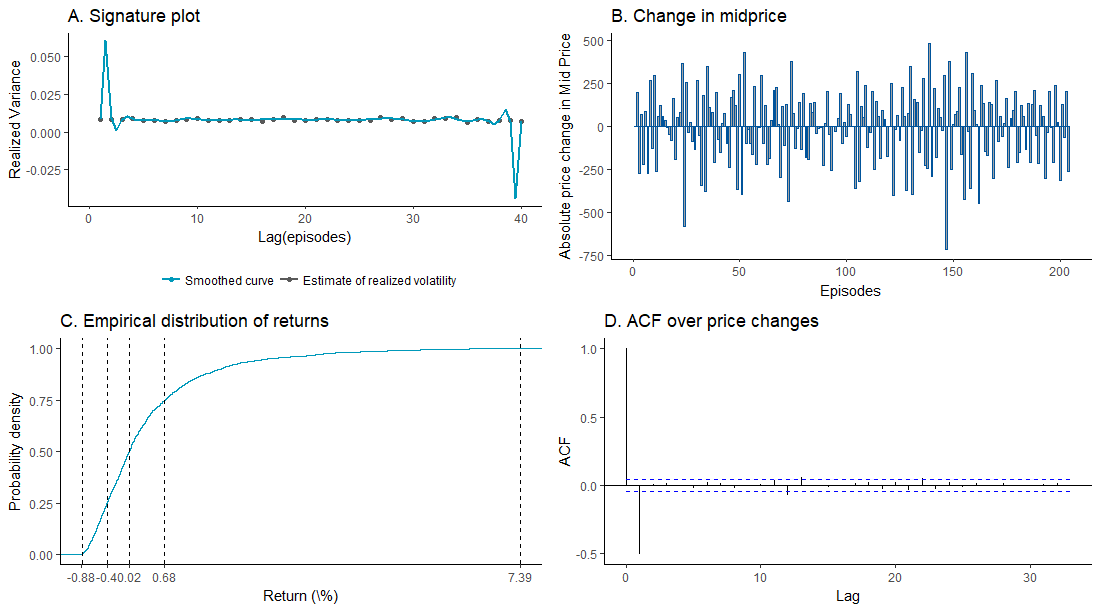
\includegraphics[scale=.35]{dmv1_sf_multi.png}
		%Captions and Labels can be used since this is a figure environment
		\caption{Stylized facts for DealerMarket-v2. Inline with \parencite{cont2001empirical, bouchaud2018trades}}
		\label{fig:sf1}
\end{figure}
  
\end{frame}

\subsection{ Dealer Agent's Rewards}

\begin{frame}[shrink=10]
  \frametitle{\hfill Dealer Agent's Rewards}
  
  \subsection*{Episode reward vs. random policy}
    \begin{figure}[H]
    		%Do not try to scale figure in .tex or you loose font size consistency
    	    	\centering
    		%The code to input the plot is extremely simple
    		% Created by tikzDevice version 0.11 on 2018-09-18 21:48:43
% !TEX encoding = UTF-8 Unicode
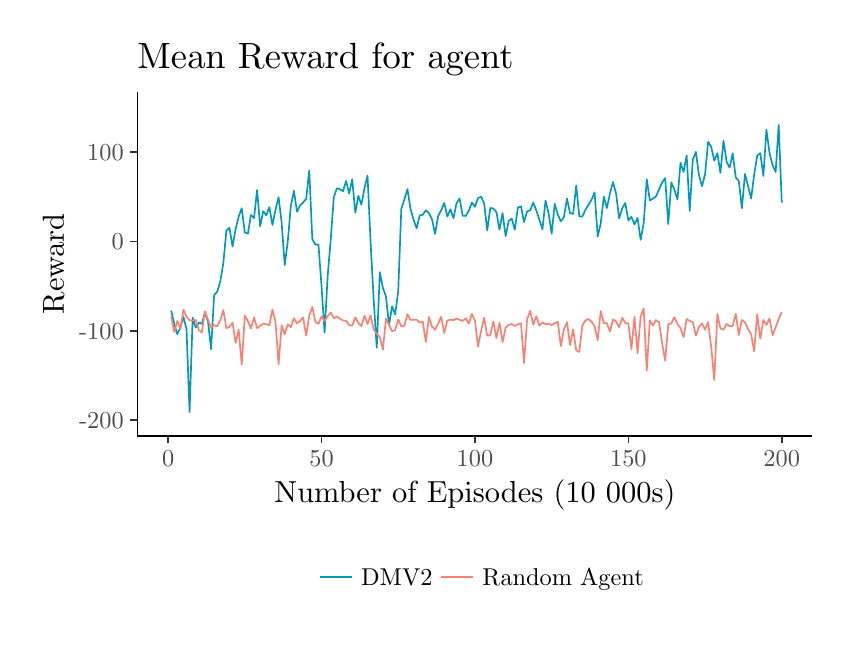
\begin{tikzpicture}[x=1pt,y=1pt]
\definecolor{fillColor}{RGB}{255,255,255}
\path[use as bounding box,fill=fillColor,fill opacity=0.00] (0,0) rectangle (289.08,216.81);
\begin{scope}
\path[clip] (  0.00,  0.00) rectangle (289.08,216.81);
\definecolor{drawColor}{RGB}{255,255,255}
\definecolor{fillColor}{RGB}{255,255,255}

\path[draw=drawColor,line width= 0.6pt,line join=round,line cap=round,fill=fillColor] (  0.00,  0.00) rectangle (289.08,216.81);
\end{scope}
\begin{scope}
\path[clip] ( 39.66, 69.30) rectangle (283.58,193.67);
\definecolor{fillColor}{RGB}{255,255,255}

\path[fill=fillColor] ( 39.66, 69.30) rectangle (283.58,193.67);
\definecolor{drawColor}{RGB}{0,153,186}

\path[draw=drawColor,line width= 0.6pt,line join=round] ( 51.85,114.58) --
	( 52.96,109.81) --
	( 54.07,106.01) --
	( 55.18,108.48) --
	( 56.29,112.28) --
	( 57.40,107.87) --
	( 58.50, 77.91) --
	( 59.61,112.01) --
	( 60.72,108.43) --
	( 61.83,110.21) --
	( 62.94,109.79) --
	( 64.05,113.77) --
	( 65.16,110.70) --
	( 66.27,100.64) --
	( 67.37,120.14) --
	( 68.48,121.39) --
	( 69.59,125.05) --
	( 70.70,131.77) --
	( 71.81,143.53) --
	( 72.92,144.46) --
	( 74.03,137.71) --
	( 75.14,144.04) --
	( 76.24,148.53) --
	( 77.35,151.56) --
	( 78.46,142.84) --
	( 79.57,142.36) --
	( 80.68,149.14) --
	( 81.79,147.99) --
	( 82.90,158.14) --
	( 84.01,145.03) --
	( 85.11,150.51) --
	( 86.22,149.00) --
	( 87.33,151.97) --
	( 88.44,145.51) --
	( 89.55,150.89) --
	( 90.66,155.57) --
	( 91.77,146.41) --
	( 92.88,131.04) --
	( 93.98,139.49) --
	( 95.09,152.38) --
	( 96.20,157.87) --
	( 97.31,150.29) --
	( 98.42,152.56) --
	( 99.53,153.63) --
	(100.64,155.02) --
	(101.75,165.22) --
	(102.85,140.41) --
	(103.96,138.41) --
	(105.07,138.48) --
	(106.18,123.50) --
	(107.29,106.65) --
	(108.40,127.07) --
	(109.51,140.26) --
	(110.62,155.49) --
	(111.72,158.77) --
	(112.83,158.46) --
	(113.94,157.70) --
	(115.05,161.42) --
	(116.16,156.88) --
	(117.27,162.01) --
	(118.38,149.96) --
	(119.49,156.03) --
	(120.59,152.82) --
	(121.70,158.88) --
	(122.81,163.32) --
	(123.92,139.04) --
	(125.03,118.50) --
	(126.14,101.10) --
	(127.25,128.45) --
	(128.36,122.73) --
	(129.46,119.72) --
	(130.57,109.38) --
	(131.68,116.09) --
	(132.79,113.19) --
	(133.90,121.60) --
	(135.01,151.37) --
	(136.12,154.73) --
	(137.23,158.47) --
	(138.33,151.32) --
	(139.44,147.43) --
	(140.55,144.28) --
	(141.66,148.98) --
	(142.77,149.21) --
	(143.88,150.83) --
	(144.99,149.81) --
	(146.10,147.62) --
	(147.20,142.31) --
	(148.31,148.70) --
	(149.42,150.82) --
	(150.53,153.48) --
	(151.64,148.54) --
	(152.75,151.20) --
	(153.86,147.95) --
	(154.97,153.35) --
	(156.07,155.11) --
	(157.18,148.84) --
	(158.29,148.77) --
	(159.40,150.66) --
	(160.51,153.60) --
	(161.62,152.10) --
	(162.73,155.20) --
	(163.84,155.75) --
	(164.94,153.36) --
	(166.05,143.54) --
	(167.16,151.64) --
	(168.27,151.46) --
	(169.38,150.15) --
	(170.49,143.77) --
	(171.60,149.81) --
	(172.71,141.47) --
	(173.81,146.96) --
	(174.92,147.80) --
	(176.03,143.75) --
	(177.14,151.83) --
	(178.25,152.26) --
	(179.36,146.52) --
	(180.47,150.46) --
	(181.58,150.81) --
	(182.68,153.62) --
	(183.79,150.77) --
	(184.90,147.49) --
	(186.01,143.93) --
	(187.12,154.31) --
	(188.23,149.76) --
	(189.34,142.37) --
	(190.45,153.18) --
	(191.55,149.33) --
	(192.66,146.83) --
	(193.77,148.36) --
	(194.88,155.03) --
	(195.99,149.79) --
	(197.10,149.50) --
	(198.21,159.78) --
	(199.32,148.61) --
	(200.42,148.56) --
	(201.53,150.96) --
	(202.64,152.77) --
	(203.75,154.63) --
	(204.86,157.30) --
	(205.97,141.33) --
	(207.08,146.15) --
	(208.19,155.75) --
	(209.29,151.62) --
	(210.40,156.87) --
	(211.51,161.04) --
	(212.62,156.86) --
	(213.73,147.91) --
	(214.84,151.55) --
	(215.95,153.45) --
	(217.06,147.13) --
	(218.16,148.46) --
	(219.27,145.71) --
	(220.38,148.06) --
	(221.49,140.15) --
	(222.60,146.19) --
	(223.71,161.98) --
	(224.82,154.38) --
	(225.93,155.02) --
	(227.03,155.83) --
	(228.14,158.31) --
	(229.25,160.89) --
	(230.36,162.44) --
	(231.47,145.88) --
	(232.58,160.88) --
	(233.69,158.28) --
	(234.80,154.73) --
	(235.90,167.99) --
	(237.01,164.69) --
	(238.12,170.63) --
	(239.23,150.60) --
	(240.34,169.15) --
	(241.45,171.94) --
	(242.56,163.54) --
	(243.67,159.52) --
	(244.77,163.88) --
	(245.88,175.56) --
	(246.99,173.76) --
	(248.10,168.73) --
	(249.21,171.46) --
	(250.32,164.34) --
	(251.43,175.97) --
	(252.54,168.40) --
	(253.64,166.24) --
	(254.75,171.41) --
	(255.86,162.75) --
	(256.97,161.37) --
	(258.08,151.56) --
	(259.19,163.93) --
	(260.30,159.63) --
	(261.41,155.04) --
	(262.51,163.66) --
	(263.62,170.61) --
	(264.73,171.47) --
	(265.84,163.22) --
	(266.95,179.96) --
	(268.06,171.53) --
	(269.17,167.20) --
	(270.28,164.64) --
	(271.38,181.67) --
	(272.49,153.57);
\definecolor{drawColor}{RGB}{250,128,114}

\path[draw=drawColor,line width= 0.6pt,line join=round] ( 51.85,112.52) --
	( 52.96,106.90) --
	( 54.07,110.84) --
	( 55.18,108.03) --
	( 56.29,114.91) --
	( 57.40,112.32) --
	( 58.50,111.08) --
	( 59.61,110.99) --
	( 60.72,111.22) --
	( 61.83,107.61) --
	( 62.94,106.64) --
	( 64.05,114.34) --
	( 65.16,111.33) --
	( 66.27,108.30) --
	( 67.37,109.35) --
	( 68.48,108.86) --
	( 69.59,111.13) --
	( 70.70,114.71) --
	( 71.81,108.23) --
	( 72.92,108.69) --
	( 74.03,110.28) --
	( 75.14,102.88) --
	( 76.24,107.76) --
	( 77.35, 94.97) --
	( 78.46,112.78) --
	( 79.57,110.74) --
	( 80.68,108.08) --
	( 81.79,112.09) --
	( 82.90,108.25) --
	( 84.01,109.03) --
	( 85.11,109.88) --
	( 86.22,109.64) --
	( 87.33,109.32) --
	( 88.44,114.92) --
	( 89.55,110.55) --
	( 90.66, 95.16) --
	( 91.77,109.26) --
	( 92.88,106.00) --
	( 93.98,109.62) --
	( 95.09,108.59) --
	( 96.20,111.83) --
	( 97.31,109.96) --
	( 98.42,110.77) --
	( 99.53,112.19) --
	(100.64,105.51) --
	(101.75,112.72) --
	(102.85,115.87) --
	(103.96,110.53) --
	(105.07,109.76) --
	(106.18,112.50) --
	(107.29,110.79) --
	(108.40,112.59) --
	(109.51,113.87) --
	(110.62,111.80) --
	(111.72,112.41) --
	(112.83,111.65) --
	(113.94,110.97) --
	(115.05,110.91) --
	(116.16,109.29) --
	(117.27,109.15) --
	(118.38,112.17) --
	(119.49,110.10) --
	(120.59,109.00) --
	(121.70,112.74) --
	(122.81,109.74) --
	(123.92,112.80) --
	(125.03,107.71) --
	(126.14,106.24) --
	(127.25,104.86) --
	(128.36,100.52) --
	(129.46,111.65) --
	(130.57,109.50) --
	(131.68,107.11) --
	(132.79,107.54) --
	(133.90,111.39) --
	(135.01,108.86) --
	(136.12,109.10) --
	(137.23,113.32) --
	(138.33,111.19) --
	(139.44,111.28) --
	(140.55,111.32) --
	(141.66,110.24) --
	(142.77,110.55) --
	(143.88,103.29) --
	(144.99,112.25) --
	(146.10,108.85) --
	(147.20,107.67) --
	(148.31,109.85) --
	(149.42,112.35) --
	(150.53,106.45) --
	(151.64,111.01) --
	(152.75,111.28) --
	(153.86,111.14) --
	(154.97,111.72) --
	(156.07,111.23) --
	(157.18,110.87) --
	(158.29,111.79) --
	(159.40,109.82) --
	(160.51,113.36) --
	(161.62,110.99) --
	(162.73,101.59) --
	(163.84,107.28) --
	(164.94,112.00) --
	(166.05,105.52) --
	(167.16,105.61) --
	(168.27,110.70) --
	(169.38,104.64) --
	(170.49,110.24) --
	(171.60,103.18) --
	(172.71,108.42) --
	(173.81,109.35) --
	(174.92,109.74) --
	(176.03,109.04) --
	(177.14,109.59) --
	(178.25,110.01) --
	(179.36, 95.62) --
	(180.47,111.41) --
	(181.58,114.49) --
	(182.68,109.57) --
	(183.79,112.58) --
	(184.90,109.13) --
	(186.01,110.29) --
	(187.12,109.71) --
	(188.23,109.80) --
	(189.34,109.37) --
	(190.45,109.95) --
	(191.55,110.56) --
	(192.66,101.72) --
	(193.77,107.75) --
	(194.88,110.39) --
	(195.99,102.12) --
	(197.10,107.75) --
	(198.21,100.19) --
	(199.32, 99.62) --
	(200.42,109.16) --
	(201.53,111.02) --
	(202.64,111.49) --
	(203.75,110.60) --
	(204.86,108.84) --
	(205.97,103.90) --
	(207.08,114.40) --
	(208.19,110.03) --
	(209.29,110.08) --
	(210.40,106.97) --
	(211.51,111.43) --
	(212.62,110.65) --
	(213.73,108.57) --
	(214.84,111.96) --
	(215.95,110.07) --
	(217.06,109.99) --
	(218.16,100.65) --
	(219.27,112.36) --
	(220.38, 99.18) --
	(221.49,112.41) --
	(222.60,115.32) --
	(223.71, 92.92) --
	(224.82,111.04) --
	(225.93,109.12) --
	(227.03,111.17) --
	(228.14,110.34) --
	(229.25,102.92) --
	(230.36, 96.47) --
	(231.47,109.52) --
	(232.58,110.00) --
	(233.69,112.20) --
	(234.80,109.66) --
	(235.90,108.30) --
	(237.01,104.98) --
	(238.12,111.55) --
	(239.23,110.88) --
	(240.34,110.35) --
	(241.45,105.52) --
	(242.56,108.67) --
	(243.67,109.98) --
	(244.77,107.69) --
	(245.88,110.41) --
	(246.99,101.42) --
	(248.10, 89.52) --
	(249.21,113.32) --
	(250.32,108.18) --
	(251.43,107.66) --
	(252.54,109.78) --
	(253.64,108.87) --
	(254.75,109.01) --
	(255.86,113.42) --
	(256.97,105.76) --
	(258.08,111.20) --
	(259.19,110.32) --
	(260.30,107.90) --
	(261.41,106.11) --
	(262.51, 99.81) --
	(263.62,113.26) --
	(264.73,104.40) --
	(265.84,111.16) --
	(266.95,109.37) --
	(268.06,111.75) --
	(269.17,105.65) --
	(270.28,108.59) --
	(271.38,111.55) --
	(272.49,114.00);
\end{scope}
\begin{scope}
\path[clip] (  0.00,  0.00) rectangle (289.08,216.81);
\definecolor{drawColor}{RGB}{0,0,0}

\path[draw=drawColor,line width= 0.6pt,line join=round] ( 39.66, 69.30) --
	( 39.66,193.67);
\end{scope}
\begin{scope}
\path[clip] (  0.00,  0.00) rectangle (289.08,216.81);
\definecolor{drawColor}{gray}{0.30}

\node[text=drawColor,anchor=base east,inner sep=0pt, outer sep=0pt, scale=  0.88] at ( 34.71, 71.93) {-200};

\node[text=drawColor,anchor=base east,inner sep=0pt, outer sep=0pt, scale=  0.88] at ( 34.71,104.23) {-100};

\node[text=drawColor,anchor=base east,inner sep=0pt, outer sep=0pt, scale=  0.88] at ( 34.71,136.53) {0};

\node[text=drawColor,anchor=base east,inner sep=0pt, outer sep=0pt, scale=  0.88] at ( 34.71,168.84) {100};
\end{scope}
\begin{scope}
\path[clip] (  0.00,  0.00) rectangle (289.08,216.81);
\definecolor{drawColor}{gray}{0.20}

\path[draw=drawColor,line width= 0.6pt,line join=round] ( 36.91, 74.96) --
	( 39.66, 74.96);

\path[draw=drawColor,line width= 0.6pt,line join=round] ( 36.91,107.26) --
	( 39.66,107.26);

\path[draw=drawColor,line width= 0.6pt,line join=round] ( 36.91,139.56) --
	( 39.66,139.56);

\path[draw=drawColor,line width= 0.6pt,line join=round] ( 36.91,171.87) --
	( 39.66,171.87);
\end{scope}
\begin{scope}
\path[clip] (  0.00,  0.00) rectangle (289.08,216.81);
\definecolor{drawColor}{RGB}{0,0,0}

\path[draw=drawColor,line width= 0.6pt,line join=round] ( 39.66, 69.30) --
	(283.58, 69.30);
\end{scope}
\begin{scope}
\path[clip] (  0.00,  0.00) rectangle (289.08,216.81);
\definecolor{drawColor}{gray}{0.20}

\path[draw=drawColor,line width= 0.6pt,line join=round] ( 50.74, 66.55) --
	( 50.74, 69.30);

\path[draw=drawColor,line width= 0.6pt,line join=round] (106.18, 66.55) --
	(106.18, 69.30);

\path[draw=drawColor,line width= 0.6pt,line join=round] (161.62, 66.55) --
	(161.62, 69.30);

\path[draw=drawColor,line width= 0.6pt,line join=round] (217.06, 66.55) --
	(217.06, 69.30);

\path[draw=drawColor,line width= 0.6pt,line join=round] (272.49, 66.55) --
	(272.49, 69.30);
\end{scope}
\begin{scope}
\path[clip] (  0.00,  0.00) rectangle (289.08,216.81);
\definecolor{drawColor}{gray}{0.30}

\node[text=drawColor,anchor=base,inner sep=0pt, outer sep=0pt, scale=  0.88] at ( 50.74, 58.29) {0};

\node[text=drawColor,anchor=base,inner sep=0pt, outer sep=0pt, scale=  0.88] at (106.18, 58.29) {50};

\node[text=drawColor,anchor=base,inner sep=0pt, outer sep=0pt, scale=  0.88] at (161.62, 58.29) {100};

\node[text=drawColor,anchor=base,inner sep=0pt, outer sep=0pt, scale=  0.88] at (217.06, 58.29) {150};

\node[text=drawColor,anchor=base,inner sep=0pt, outer sep=0pt, scale=  0.88] at (272.49, 58.29) {200};
\end{scope}
\begin{scope}
\path[clip] (  0.00,  0.00) rectangle (289.08,216.81);
\definecolor{drawColor}{RGB}{0,0,0}

\node[text=drawColor,anchor=base,inner sep=0pt, outer sep=0pt, scale=  1.10] at (161.62, 45.22) {Number of Episodes (10 000s)};
\end{scope}
\begin{scope}
\path[clip] (  0.00,  0.00) rectangle (289.08,216.81);
\definecolor{drawColor}{RGB}{0,0,0}

\node[text=drawColor,rotate= 90.00,anchor=base,inner sep=0pt, outer sep=0pt, scale=  1.10] at ( 13.08,131.49) {Reward};
\end{scope}
\begin{scope}
\path[clip] (  0.00,  0.00) rectangle (289.08,216.81);
\definecolor{fillColor}{RGB}{255,255,255}

\path[fill=fillColor] ( 94.92,  5.50) rectangle (228.31, 31.34);
\end{scope}
\begin{scope}
\path[clip] (  0.00,  0.00) rectangle (289.08,216.81);
\definecolor{drawColor}{RGB}{0,153,186}

\path[draw=drawColor,line width= 0.6pt,line join=round] (105.67, 18.42) -- (117.23, 18.42);
\end{scope}
\begin{scope}
\path[clip] (  0.00,  0.00) rectangle (289.08,216.81);
\definecolor{drawColor}{RGB}{250,128,114}

\path[draw=drawColor,line width= 0.6pt,line join=round] (149.52, 18.42) -- (161.08, 18.42);
\end{scope}
\begin{scope}
\path[clip] (  0.00,  0.00) rectangle (289.08,216.81);
\definecolor{drawColor}{RGB}{0,0,0}

\node[text=drawColor,anchor=base west,inner sep=0pt, outer sep=0pt, scale=  0.88] at (120.49, 15.39) {DMV2};
\end{scope}
\begin{scope}
\path[clip] (  0.00,  0.00) rectangle (289.08,216.81);
\definecolor{drawColor}{RGB}{0,0,0}

\node[text=drawColor,anchor=base west,inner sep=0pt, outer sep=0pt, scale=  0.88] at (164.34, 15.39) {Random Agent};
\end{scope}
\begin{scope}
\path[clip] (  0.00,  0.00) rectangle (289.08,216.81);
\definecolor{drawColor}{RGB}{0,0,0}

\node[text=drawColor,anchor=base west,inner sep=0pt, outer sep=0pt, scale=  1.32] at ( 39.66,202.22) {Mean Reward for agent};
\end{scope}
\end{tikzpicture}

    		%Captions and Labels can be used since this is a figure environment
    		\caption{ \small Average reward after training DealerMarket-v2.}
    		\label{fig:dm1}
    \end{figure}
  
\end{frame}

\subsection{ LOB Agent's Rewards}

\begin{frame}[shrink=10]
  \frametitle{\hfill LOB Agent's Rewards}
  
  \subsection*{Episode reward vs. random policy}
    \begin{figure}[H]
    		%Do not try to scale figure in .tex or you loose font size consistency
    	    	\centering
    		%The code to input the plot is extremely simple
    		% Created by tikzDevice version 0.11 on 2018-09-18 21:57:12
% !TEX encoding = UTF-8 Unicode
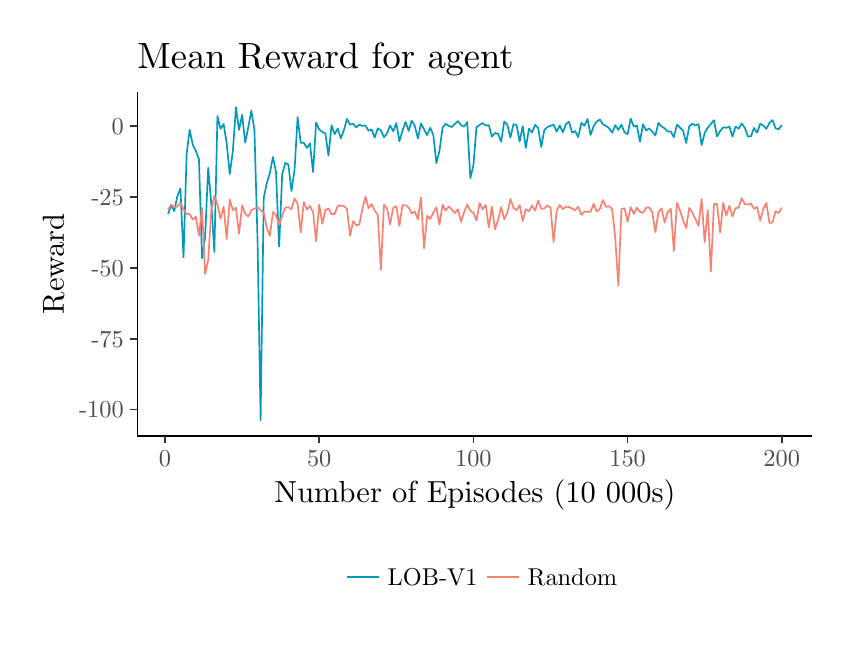
\begin{tikzpicture}[x=1pt,y=1pt]
\definecolor{fillColor}{RGB}{255,255,255}
\path[use as bounding box,fill=fillColor,fill opacity=0.00] (0,0) rectangle (289.08,216.81);
\begin{scope}
\path[clip] (  0.00,  0.00) rectangle (289.08,216.81);
\definecolor{drawColor}{RGB}{255,255,255}
\definecolor{fillColor}{RGB}{255,255,255}

\path[draw=drawColor,line width= 0.6pt,line join=round,line cap=round,fill=fillColor] (  0.00,  0.00) rectangle (289.08,216.81);
\end{scope}
\begin{scope}
\path[clip] ( 39.66, 69.30) rectangle (283.58,193.67);
\definecolor{fillColor}{RGB}{255,255,255}

\path[fill=fillColor] ( 39.66, 69.30) rectangle (283.58,193.67);
\definecolor{drawColor}{RGB}{0,153,186}

\path[draw=drawColor,line width= 0.6pt,line join=round] ( 50.74,149.45) --
	( 51.86,152.74) --
	( 52.97,150.53) --
	( 54.09,155.94) --
	( 55.20,158.67) --
	( 56.31,133.79) --
	( 57.43,171.06) --
	( 58.54,179.94) --
	( 59.66,174.46) --
	( 60.77,172.32) --
	( 61.89,169.20) --
	( 63.00,133.45) --
	( 64.11,141.05) --
	( 65.23,166.20) --
	( 66.34,153.19) --
	( 67.46,135.71) --
	( 68.57,184.84) --
	( 69.69,180.27) --
	( 70.80,181.99) --
	( 71.91,175.05) --
	( 73.03,163.92) --
	( 74.14,172.20) --
	( 75.26,188.02) --
	( 76.37,179.89) --
	( 77.49,185.32) --
	( 78.60,175.25) --
	( 79.72,180.82) --
	( 80.83,186.82) --
	( 81.94,179.74) --
	( 83.06,140.08) --
	( 84.17, 74.96) --
	( 85.29,155.28) --
	( 86.40,160.60) --
	( 87.52,164.31) --
	( 88.63,170.08) --
	( 89.74,164.57) --
	( 90.86,137.68) --
	( 91.97,163.84) --
	( 93.09,167.93) --
	( 94.20,167.32) --
	( 95.32,157.78) --
	( 96.43,165.32) --
	( 97.54,184.52) --
	( 98.66,175.23) --
	( 99.77,175.23) --
	(100.89,173.33) --
	(102.00,175.01) --
	(103.12,164.64) --
	(104.23,182.56) --
	(105.34,180.07) --
	(106.46,179.16) --
	(107.57,178.56) --
	(108.69,170.57) --
	(109.80,181.55) --
	(110.92,178.31) --
	(112.03,180.35) --
	(113.14,176.82) --
	(114.26,179.77) --
	(115.37,183.82) --
	(116.49,181.79) --
	(117.60,182.06) --
	(118.72,180.78) --
	(119.83,181.77) --
	(120.95,181.33) --
	(122.06,181.48) --
	(123.17,179.55) --
	(124.29,180.01) --
	(125.40,177.11) --
	(126.52,180.44) --
	(127.63,179.72) --
	(128.75,177.18) --
	(129.86,178.66) --
	(130.97,181.45) --
	(132.09,179.36) --
	(133.20,182.30) --
	(134.32,175.74) --
	(135.43,179.58) --
	(136.55,182.77) --
	(137.66,179.50) --
	(138.77,183.21) --
	(139.89,181.28) --
	(141.00,176.80) --
	(142.12,182.20) --
	(143.23,180.07) --
	(144.35,178.00) --
	(145.46,180.64) --
	(146.57,178.03) --
	(147.69,167.85) --
	(148.80,172.33) --
	(149.92,180.69) --
	(151.03,182.08) --
	(152.15,181.32) --
	(153.26,180.91) --
	(154.37,182.07) --
	(155.49,183.04) --
	(156.60,181.61) --
	(157.72,181.03) --
	(158.83,182.70) --
	(159.95,162.44) --
	(161.06,167.05) --
	(162.17,180.84) --
	(163.29,181.61) --
	(164.40,182.33) --
	(165.52,181.44) --
	(166.63,181.61) --
	(167.75,177.41) --
	(168.86,178.77) --
	(169.98,178.43) --
	(171.09,175.61) --
	(172.20,182.94) --
	(173.32,181.72) --
	(174.43,177.11) --
	(175.55,181.93) --
	(176.66,181.61) --
	(177.78,175.62) --
	(178.89,181.23) --
	(180.00,173.34) --
	(181.12,180.29) --
	(182.23,178.91) --
	(183.35,181.68) --
	(184.46,180.61) --
	(185.58,173.70) --
	(186.69,179.83) --
	(187.80,180.86) --
	(188.92,181.33) --
	(190.03,181.83) --
	(191.15,179.22) --
	(192.26,181.48) --
	(193.38,178.99) --
	(194.49,181.93) --
	(195.60,182.88) --
	(196.72,178.91) --
	(197.83,179.46) --
	(198.95,177.22) --
	(200.06,182.41) --
	(201.18,181.36) --
	(202.29,183.82) --
	(203.40,178.04) --
	(204.52,181.27) --
	(205.63,182.86) --
	(206.75,183.62) --
	(207.86,181.91) --
	(208.98,181.33) --
	(210.09,180.47) --
	(211.20,178.84) --
	(212.32,181.57) --
	(213.43,179.87) --
	(214.55,181.78) --
	(215.66,178.99) --
	(216.78,178.29) --
	(217.89,183.95) --
	(219.01,181.09) --
	(220.12,181.47) --
	(221.23,175.60) --
	(222.35,181.85) --
	(223.46,179.65) --
	(224.58,180.41) --
	(225.69,179.27) --
	(226.81,177.86) --
	(227.92,182.40) --
	(229.03,181.13) --
	(230.15,180.45) --
	(231.26,179.33) --
	(232.38,179.30) --
	(233.49,177.22) --
	(234.61,181.78) --
	(235.72,180.67) --
	(236.83,179.60) --
	(237.95,175.16) --
	(239.06,181.17) --
	(240.18,182.08) --
	(241.29,181.48) --
	(242.41,181.92) --
	(243.52,174.38) --
	(244.63,178.73) --
	(245.75,180.68) --
	(246.86,181.99) --
	(247.98,183.37) --
	(249.09,177.50) --
	(250.21,179.43) --
	(251.32,180.79) --
	(252.43,180.64) --
	(253.55,181.09) --
	(254.66,177.43) --
	(255.78,181.09) --
	(256.89,180.31) --
	(258.01,182.18) --
	(259.12,180.66) --
	(260.24,177.49) --
	(261.35,177.54) --
	(262.46,180.58) --
	(263.58,178.83) --
	(264.69,182.11) --
	(265.81,181.46) --
	(266.92,180.23) --
	(268.04,182.46) --
	(269.15,183.41) --
	(270.26,180.44) --
	(271.38,180.09) --
	(272.49,181.61);
\definecolor{drawColor}{RGB}{250,128,114}

\path[draw=drawColor,line width= 0.6pt,line join=round] ( 50.74,151.04) --
	( 51.86,152.89) --
	( 52.97,151.90) --
	( 54.09,152.19) --
	( 55.20,153.56) --
	( 56.31,151.09) --
	( 57.43,149.49) --
	( 58.54,149.44) --
	( 59.66,147.45) --
	( 60.77,148.47) --
	( 61.89,141.62) --
	( 63.00,151.74) --
	( 64.11,127.78) --
	( 65.23,132.79) --
	( 66.34,150.83) --
	( 67.46,156.02) --
	( 68.57,152.93) --
	( 69.69,147.75) --
	( 70.80,152.09) --
	( 71.91,140.50) --
	( 73.03,154.69) --
	( 74.14,150.86) --
	( 75.26,151.77) --
	( 76.37,142.33) --
	( 77.49,152.61) --
	( 78.60,149.50) --
	( 79.72,148.58) --
	( 80.83,150.91) --
	( 81.94,151.38) --
	( 83.06,152.00) --
	( 84.17,150.90) --
	( 85.29,150.10) --
	( 86.40,144.47) --
	( 87.52,141.60) --
	( 88.63,150.21) --
	( 89.74,149.05) --
	( 90.86,145.56) --
	( 91.97,149.00) --
	( 93.09,151.82) --
	( 94.20,151.92) --
	( 95.32,151.20) --
	( 96.43,155.15) --
	( 97.54,153.12) --
	( 98.66,142.78) --
	( 99.77,153.79) --
	(100.89,151.07) --
	(102.00,152.37) --
	(103.12,150.18) --
	(104.23,139.63) --
	(105.34,152.92) --
	(106.46,145.95) --
	(107.57,150.86) --
	(108.69,151.49) --
	(109.80,149.40) --
	(110.92,149.49) --
	(112.03,152.34) --
	(113.14,152.54) --
	(114.26,152.38) --
	(115.37,151.33) --
	(116.49,141.68) --
	(117.60,146.91) --
	(118.72,145.42) --
	(119.83,145.66) --
	(120.95,151.30) --
	(122.06,155.74) --
	(123.17,151.54) --
	(124.29,153.05) --
	(125.40,150.70) --
	(126.52,149.23) --
	(127.63,129.32) --
	(128.75,152.80) --
	(129.86,151.54) --
	(130.97,145.73) --
	(132.09,151.70) --
	(133.20,152.24) --
	(134.32,145.20) --
	(135.43,152.72) --
	(136.55,152.59) --
	(137.66,151.85) --
	(138.77,149.64) --
	(139.89,150.39) --
	(141.00,147.55) --
	(142.12,155.46) --
	(143.23,137.05) --
	(144.35,148.80) --
	(145.46,147.74) --
	(146.57,149.98) --
	(147.69,151.89) --
	(148.80,145.64) --
	(149.92,152.81) --
	(151.03,150.69) --
	(152.15,152.22) --
	(153.26,151.09) --
	(154.37,149.82) --
	(155.49,151.18) --
	(156.60,146.60) --
	(157.72,150.21) --
	(158.83,152.91) --
	(159.95,150.66) --
	(161.06,149.95) --
	(162.17,147.11) --
	(163.29,153.44) --
	(164.40,151.20) --
	(165.52,152.74) --
	(166.63,144.55) --
	(167.75,152.15) --
	(168.86,143.92) --
	(169.98,147.28) --
	(171.09,151.98) --
	(172.20,147.60) --
	(173.32,149.92) --
	(174.43,154.92) --
	(175.55,151.66) --
	(176.66,150.87) --
	(177.78,152.66) --
	(178.89,146.90) --
	(180.00,151.22) --
	(181.12,150.46) --
	(182.23,152.54) --
	(183.35,150.66) --
	(184.46,154.40) --
	(185.58,151.36) --
	(186.69,151.48) --
	(187.80,152.60) --
	(188.92,151.79) --
	(190.03,139.36) --
	(191.15,150.67) --
	(192.26,152.72) --
	(193.38,151.22) --
	(194.49,152.12) --
	(195.60,152.00) --
	(196.72,151.39) --
	(197.83,150.83) --
	(198.95,152.11) --
	(200.06,149.18) --
	(201.18,150.38) --
	(202.29,150.27) --
	(203.40,150.27) --
	(204.52,153.16) --
	(205.63,150.37) --
	(206.75,151.34) --
	(207.86,154.54) --
	(208.98,152.07) --
	(210.09,152.33) --
	(211.20,151.19) --
	(212.32,140.78) --
	(213.43,123.62) --
	(214.55,151.32) --
	(215.66,151.53) --
	(216.78,146.67) --
	(217.89,151.94) --
	(219.01,149.53) --
	(220.12,151.73) --
	(221.23,150.24) --
	(222.35,149.92) --
	(223.46,151.72) --
	(224.58,151.87) --
	(225.69,150.11) --
	(226.81,142.91) --
	(227.92,150.10) --
	(229.03,151.53) --
	(230.15,146.39) --
	(231.26,150.11) --
	(232.38,151.42) --
	(233.49,136.10) --
	(234.61,153.53) --
	(235.72,150.65) --
	(236.83,147.32) --
	(237.95,144.38) --
	(239.06,151.72) --
	(240.18,149.94) --
	(241.29,147.64) --
	(242.41,145.21) --
	(243.52,154.95) --
	(244.63,139.32) --
	(245.75,150.95) --
	(246.86,128.69) --
	(247.98,153.06) --
	(249.09,153.12) --
	(250.21,142.79) --
	(251.32,153.54) --
	(252.43,148.93) --
	(253.55,152.47) --
	(254.66,148.63) --
	(255.78,151.59) --
	(256.89,151.76) --
	(258.01,155.20) --
	(259.12,153.07) --
	(260.24,152.85) --
	(261.35,153.24) --
	(262.46,151.35) --
	(263.58,152.04) --
	(264.69,147.13) --
	(265.81,151.38) --
	(266.92,153.46) --
	(268.04,146.23) --
	(269.15,146.51) --
	(270.26,150.48) --
	(271.38,149.83) --
	(272.49,151.82);
\end{scope}
\begin{scope}
\path[clip] (  0.00,  0.00) rectangle (289.08,216.81);
\definecolor{drawColor}{RGB}{0,0,0}

\path[draw=drawColor,line width= 0.6pt,line join=round] ( 39.66, 69.30) --
	( 39.66,193.67);
\end{scope}
\begin{scope}
\path[clip] (  0.00,  0.00) rectangle (289.08,216.81);
\definecolor{drawColor}{gray}{0.30}

\node[text=drawColor,anchor=base east,inner sep=0pt, outer sep=0pt, scale=  0.88] at ( 34.71, 75.78) {-100};

\node[text=drawColor,anchor=base east,inner sep=0pt, outer sep=0pt, scale=  0.88] at ( 34.71,101.38) {-75};

\node[text=drawColor,anchor=base east,inner sep=0pt, outer sep=0pt, scale=  0.88] at ( 34.71,126.97) {-50};

\node[text=drawColor,anchor=base east,inner sep=0pt, outer sep=0pt, scale=  0.88] at ( 34.71,152.56) {-25};

\node[text=drawColor,anchor=base east,inner sep=0pt, outer sep=0pt, scale=  0.88] at ( 34.71,178.15) {0};
\end{scope}
\begin{scope}
\path[clip] (  0.00,  0.00) rectangle (289.08,216.81);
\definecolor{drawColor}{gray}{0.20}

\path[draw=drawColor,line width= 0.6pt,line join=round] ( 36.91, 78.81) --
	( 39.66, 78.81);

\path[draw=drawColor,line width= 0.6pt,line join=round] ( 36.91,104.41) --
	( 39.66,104.41);

\path[draw=drawColor,line width= 0.6pt,line join=round] ( 36.91,130.00) --
	( 39.66,130.00);

\path[draw=drawColor,line width= 0.6pt,line join=round] ( 36.91,155.59) --
	( 39.66,155.59);

\path[draw=drawColor,line width= 0.6pt,line join=round] ( 36.91,181.18) --
	( 39.66,181.18);
\end{scope}
\begin{scope}
\path[clip] (  0.00,  0.00) rectangle (289.08,216.81);
\definecolor{drawColor}{RGB}{0,0,0}

\path[draw=drawColor,line width= 0.6pt,line join=round] ( 39.66, 69.30) --
	(283.58, 69.30);
\end{scope}
\begin{scope}
\path[clip] (  0.00,  0.00) rectangle (289.08,216.81);
\definecolor{drawColor}{gray}{0.20}

\path[draw=drawColor,line width= 0.6pt,line join=round] ( 49.63, 66.55) --
	( 49.63, 69.30);

\path[draw=drawColor,line width= 0.6pt,line join=round] (105.34, 66.55) --
	(105.34, 69.30);

\path[draw=drawColor,line width= 0.6pt,line join=round] (161.06, 66.55) --
	(161.06, 69.30);

\path[draw=drawColor,line width= 0.6pt,line join=round] (216.78, 66.55) --
	(216.78, 69.30);

\path[draw=drawColor,line width= 0.6pt,line join=round] (272.49, 66.55) --
	(272.49, 69.30);
\end{scope}
\begin{scope}
\path[clip] (  0.00,  0.00) rectangle (289.08,216.81);
\definecolor{drawColor}{gray}{0.30}

\node[text=drawColor,anchor=base,inner sep=0pt, outer sep=0pt, scale=  0.88] at ( 49.63, 58.29) {0};

\node[text=drawColor,anchor=base,inner sep=0pt, outer sep=0pt, scale=  0.88] at (105.34, 58.29) {50};

\node[text=drawColor,anchor=base,inner sep=0pt, outer sep=0pt, scale=  0.88] at (161.06, 58.29) {100};

\node[text=drawColor,anchor=base,inner sep=0pt, outer sep=0pt, scale=  0.88] at (216.78, 58.29) {150};

\node[text=drawColor,anchor=base,inner sep=0pt, outer sep=0pt, scale=  0.88] at (272.49, 58.29) {200};
\end{scope}
\begin{scope}
\path[clip] (  0.00,  0.00) rectangle (289.08,216.81);
\definecolor{drawColor}{RGB}{0,0,0}

\node[text=drawColor,anchor=base,inner sep=0pt, outer sep=0pt, scale=  1.10] at (161.62, 45.22) {Number of Episodes (10 000s)};
\end{scope}
\begin{scope}
\path[clip] (  0.00,  0.00) rectangle (289.08,216.81);
\definecolor{drawColor}{RGB}{0,0,0}

\node[text=drawColor,rotate= 90.00,anchor=base,inner sep=0pt, outer sep=0pt, scale=  1.10] at ( 13.08,131.49) {Reward};
\end{scope}
\begin{scope}
\path[clip] (  0.00,  0.00) rectangle (289.08,216.81);
\definecolor{fillColor}{RGB}{255,255,255}

\path[fill=fillColor] (104.51,  5.50) rectangle (218.72, 31.34);
\end{scope}
\begin{scope}
\path[clip] (  0.00,  0.00) rectangle (289.08,216.81);
\definecolor{drawColor}{RGB}{0,153,186}

\path[draw=drawColor,line width= 0.6pt,line join=round] (115.26, 18.42) -- (126.83, 18.42);
\end{scope}
\begin{scope}
\path[clip] (  0.00,  0.00) rectangle (289.08,216.81);
\definecolor{drawColor}{RGB}{250,128,114}

\path[draw=drawColor,line width= 0.6pt,line join=round] (165.83, 18.42) -- (177.40, 18.42);
\end{scope}
\begin{scope}
\path[clip] (  0.00,  0.00) rectangle (289.08,216.81);
\definecolor{drawColor}{RGB}{0,0,0}

\node[text=drawColor,anchor=base west,inner sep=0pt, outer sep=0pt, scale=  0.88] at (130.08, 15.39) {LOB-V1};
\end{scope}
\begin{scope}
\path[clip] (  0.00,  0.00) rectangle (289.08,216.81);
\definecolor{drawColor}{RGB}{0,0,0}

\node[text=drawColor,anchor=base west,inner sep=0pt, outer sep=0pt, scale=  0.88] at (180.65, 15.39) {Random};
\end{scope}
\begin{scope}
\path[clip] (  0.00,  0.00) rectangle (289.08,216.81);
\definecolor{drawColor}{RGB}{0,0,0}

\node[text=drawColor,anchor=base west,inner sep=0pt, outer sep=0pt, scale=  1.32] at ( 39.66,202.22) {Mean Reward for agent};
\end{scope}
\end{tikzpicture}

    		%Captions and Labels can be used since this is a figure environment
    		\caption{ \small Average reward after training LOBMarket-v1.}
    		\label{fig:p1}
    \end{figure}
  
\end{frame}

\subsection{Prices \& Inventory}

\begin{frame}[shrink=10]
  \frametitle{\hfill Prices \& Inventory}
   \begin{figure}[H]
    		%Do not try to scale figure in .tex or you loose font size consistency
    	    	\centering
    		%The code to input the plot is extremely simple
    		% Created by tikzDevice version 0.11 on 2018-09-18 22:21:18
% !TEX encoding = UTF-8 Unicode
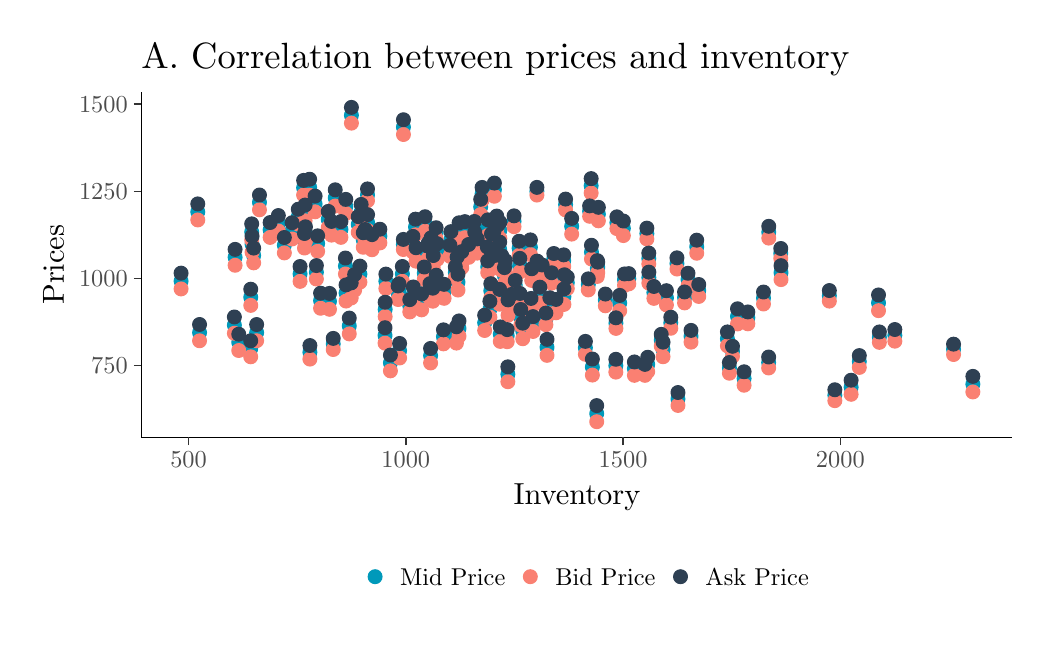
\begin{tikzpicture}[x=1pt,y=1pt]
\definecolor{fillColor}{RGB}{255,255,255}
\path[use as bounding box,fill=fillColor,fill opacity=0.00] (0,0) rectangle (361.35,216.81);
\begin{scope}
\path[clip] (  0.00,  0.00) rectangle (361.35,216.81);
\definecolor{drawColor}{RGB}{255,255,255}
\definecolor{fillColor}{RGB}{255,255,255}

\path[draw=drawColor,line width= 0.6pt,line join=round,line cap=round,fill=fillColor] (  0.00,  0.00) rectangle (361.35,216.81);
\end{scope}
\begin{scope}
\path[clip] ( 41.12, 68.75) rectangle (355.85,193.67);
\definecolor{fillColor}{RGB}{255,255,255}

\path[fill=fillColor] ( 41.12, 68.75) rectangle (355.85,193.67);
\definecolor{drawColor}{RGB}{0,153,186}
\definecolor{fillColor}{RGB}{0,153,186}

\path[draw=drawColor,line width= 0.4pt,line join=round,line cap=round,fill=fillColor] (155.18,132.36) circle (  2.50);

\path[draw=drawColor,line width= 0.4pt,line join=round,line cap=round,fill=fillColor] (184.01,157.71) circle (  2.50);

\path[draw=drawColor,line width= 0.4pt,line join=round,line cap=round,fill=fillColor] (176.17,123.80) circle (  2.50);

\path[draw=drawColor,line width= 0.4pt,line join=round,line cap=round,fill=fillColor] (193.70,132.61) circle (  2.50);

\path[draw=drawColor,line width= 0.4pt,line join=round,line cap=round,fill=fillColor] (239.70,105.29) circle (  2.50);

\path[draw=drawColor,line width= 0.4pt,line join=round,line cap=round,fill=fillColor] (181.88,116.61) circle (  2.50);

\path[draw=drawColor,line width= 0.4pt,line join=round,line cap=round,fill=fillColor] (234.98, 82.63) circle (  2.50);

\path[draw=drawColor,line width= 0.4pt,line join=round,line cap=round,fill=fillColor] (138.07,116.30) circle (  2.50);

\path[draw=drawColor,line width= 0.4pt,line join=round,line cap=round,fill=fillColor] (229.59,100.54) circle (  2.50);

\path[draw=drawColor,line width= 0.4pt,line join=round,line cap=round,fill=fillColor] (162.45,137.91) circle (  2.50);

\path[draw=drawColor,line width= 0.4pt,line join=round,line cap=round,fill=fillColor] (150.24,105.09) circle (  2.50);

\path[draw=drawColor,line width= 0.4pt,line join=round,line cap=round,fill=fillColor] (256.50,112.49) circle (  2.50);

\path[draw=drawColor,line width= 0.4pt,line join=round,line cap=round,fill=fillColor] ( 98.43,127.82) circle (  2.50);

\path[draw=drawColor,line width= 0.4pt,line join=round,line cap=round,fill=fillColor] (144.41,135.35) circle (  2.50);

\path[draw=drawColor,line width= 0.4pt,line join=round,line cap=round,fill=fillColor] (161.55,140.36) circle (  2.50);

\path[draw=drawColor,line width= 0.4pt,line join=round,line cap=round,fill=fillColor] (121.27,140.08) circle (  2.50);

\path[draw=drawColor,line width= 0.4pt,line join=round,line cap=round,fill=fillColor] (140.33,134.85) circle (  2.50);

\path[draw=drawColor,line width= 0.4pt,line join=round,line cap=round,fill=fillColor] (129.43,125.16) circle (  2.50);

\path[draw=drawColor,line width= 0.4pt,line join=round,line cap=round,fill=fillColor] (143.61,145.87) circle (  2.50);

\path[draw=drawColor,line width= 0.4pt,line join=round,line cap=round,fill=fillColor] (145.37,121.71) circle (  2.50);

\path[draw=drawColor,line width= 0.4pt,line join=round,line cap=round,fill=fillColor] (104.33,128.41) circle (  2.50);

\path[draw=drawColor,line width= 0.4pt,line join=round,line cap=round,fill=fillColor] (104.78,138.80) circle (  2.50);

\path[draw=drawColor,line width= 0.4pt,line join=round,line cap=round,fill=fillColor] (116.98,185.15) circle (  2.50);

\path[draw=drawColor,line width= 0.4pt,line join=round,line cap=round,fill=fillColor] (178.17,112.14) circle (  2.50);

\path[draw=drawColor,line width= 0.4pt,line join=round,line cap=round,fill=fillColor] (166.31,144.53) circle (  2.50);

\path[draw=drawColor,line width= 0.4pt,line join=round,line cap=round,fill=fillColor] (152.93,140.22) circle (  2.50);

\path[draw=drawColor,line width= 0.4pt,line join=round,line cap=round,fill=fillColor] (170.62,143.59) circle (  2.50);

\path[draw=drawColor,line width= 0.4pt,line join=round,line cap=round,fill=fillColor] (156.86,133.00) circle (  2.50);

\path[draw=drawColor,line width= 0.4pt,line join=round,line cap=round,fill=fillColor] (188.69,116.32) circle (  2.50);

\path[draw=drawColor,line width= 0.4pt,line join=round,line cap=round,fill=fillColor] (120.50,150.17) circle (  2.50);

\path[draw=drawColor,line width= 0.4pt,line join=round,line cap=round,fill=fillColor] (157.97,143.82) circle (  2.50);

\path[draw=drawColor,line width= 0.4pt,line join=round,line cap=round,fill=fillColor] (187.66,101.30) circle (  2.50);

\path[draw=drawColor,line width= 0.4pt,line join=round,line cap=round,fill=fillColor] (147.63,124.44) circle (  2.50);

\path[draw=drawColor,line width= 0.4pt,line join=round,line cap=round,fill=fillColor] (205.62, 77.34) circle (  2.50);

\path[draw=drawColor,line width= 0.4pt,line join=round,line cap=round,fill=fillColor] (134.17,121.54) circle (  2.50);

\path[draw=drawColor,line width= 0.4pt,line join=round,line cap=round,fill=fillColor] (147.93,135.92) circle (  2.50);

\path[draw=drawColor,line width= 0.4pt,line join=round,line cap=round,fill=fillColor] (122.82,146.40) circle (  2.50);

\path[draw=drawColor,line width= 0.4pt,line join=round,line cap=round,fill=fillColor] (185.08,120.19) circle (  2.50);

\path[draw=drawColor,line width= 0.4pt,line join=round,line cap=round,fill=fillColor] (196.57,145.05) circle (  2.50);

\path[draw=drawColor,line width= 0.4pt,line join=round,line cap=round,fill=fillColor] (144.74,136.19) circle (  2.50);

\path[draw=drawColor,line width= 0.4pt,line join=round,line cap=round,fill=fillColor] (213.93,117.30) circle (  2.50);

\path[draw=drawColor,line width= 0.4pt,line join=round,line cap=round,fill=fillColor] (193.77,119.60) circle (  2.50);

\path[draw=drawColor,line width= 0.4pt,line join=round,line cap=round,fill=fillColor] (205.83,129.77) circle (  2.50);

\path[draw=drawColor,line width= 0.4pt,line join=round,line cap=round,fill=fillColor] (307.45,117.39) circle (  2.50);

\path[draw=drawColor,line width= 0.4pt,line join=round,line cap=round,fill=fillColor] (341.54, 87.99) circle (  2.50);

\path[draw=drawColor,line width= 0.4pt,line join=round,line cap=round,fill=fillColor] (182.61,109.71) circle (  2.50);

\path[draw=drawColor,line width= 0.4pt,line join=round,line cap=round,fill=fillColor] (170.57,136.63) circle (  2.50);

\path[draw=drawColor,line width= 0.4pt,line join=round,line cap=round,fill=fillColor] (163.70,152.05) circle (  2.50);

\path[draw=drawColor,line width= 0.4pt,line join=round,line cap=round,fill=fillColor] (170.78,106.06) circle (  2.50);

\path[draw=drawColor,line width= 0.4pt,line join=round,line cap=round,fill=fillColor] (215.25,144.31) circle (  2.50);

\path[draw=drawColor,line width= 0.4pt,line join=round,line cap=round,fill=fillColor] (224.05, 95.11) circle (  2.50);

\path[draw=drawColor,line width= 0.4pt,line join=round,line cap=round,fill=fillColor] (206.22,149.45) circle (  2.50);

\path[draw=drawColor,line width= 0.4pt,line join=round,line cap=round,fill=fillColor] (241.76,137.66) circle (  2.50);

\path[draw=drawColor,line width= 0.4pt,line join=round,line cap=round,fill=fillColor] (159.34,136.13) circle (  2.50);

\path[draw=drawColor,line width= 0.4pt,line join=round,line cap=round,fill=fillColor] (202.58,124.04) circle (  2.50);

\path[draw=drawColor,line width= 0.4pt,line join=round,line cap=round,fill=fillColor] (228.93,103.88) circle (  2.50);

\path[draw=drawColor,line width= 0.4pt,line join=round,line cap=round,fill=fillColor] (224.44,133.39) circle (  2.50);

\path[draw=drawColor,line width= 0.4pt,line join=round,line cap=round,fill=fillColor] (313.35,105.63) circle (  2.50);

\path[draw=drawColor,line width= 0.4pt,line join=round,line cap=round,fill=fillColor] (173.28,105.51) circle (  2.50);

\path[draw=drawColor,line width= 0.4pt,line join=round,line cap=round,fill=fillColor] (267.79,142.90) circle (  2.50);

\path[draw=drawColor,line width= 0.4pt,line join=round,line cap=round,fill=fillColor] (166.24,130.41) circle (  2.50);

\path[draw=drawColor,line width= 0.4pt,line join=round,line cap=round,fill=fillColor] (212.91,146.32) circle (  2.50);

\path[draw=drawColor,line width= 0.4pt,line join=round,line cap=round,fill=fillColor] (265.89,119.12) circle (  2.50);

\path[draw=drawColor,line width= 0.4pt,line join=round,line cap=round,fill=fillColor] (300.51, 96.18) circle (  2.50);

\path[draw=drawColor,line width= 0.4pt,line join=round,line cap=round,fill=fillColor] (201.53,101.11) circle (  2.50);

\path[draw=drawColor,line width= 0.4pt,line join=round,line cap=round,fill=fillColor] (143.31,128.08) circle (  2.50);

\path[draw=drawColor,line width= 0.4pt,line join=round,line cap=round,fill=fillColor] (164.20,156.76) circle (  2.50);

\path[draw=drawColor,line width= 0.4pt,line join=round,line cap=round,fill=fillColor] (168.65,158.27) circle (  2.50);

\path[draw=drawColor,line width= 0.4pt,line join=round,line cap=round,fill=fillColor] (133.86,121.03) circle (  2.50);

\path[draw=drawColor,line width= 0.4pt,line join=round,line cap=round,fill=fillColor] (203.72,135.70) circle (  2.50);

\path[draw=drawColor,line width= 0.4pt,line join=round,line cap=round,fill=fillColor] (242.49,121.85) circle (  2.50);

\path[draw=drawColor,line width= 0.4pt,line join=round,line cap=round,fill=fillColor] (135.75,138.47) circle (  2.50);

\path[draw=drawColor,line width= 0.4pt,line join=round,line cap=round,fill=fillColor] (291.67, 84.00) circle (  2.50);

\path[draw=drawColor,line width= 0.4pt,line join=round,line cap=round,fill=fillColor] (234.61,131.61) circle (  2.50);

\path[draw=drawColor,line width= 0.4pt,line join=round,line cap=round,fill=fillColor] (168.49,141.27) circle (  2.50);

\path[draw=drawColor,line width= 0.4pt,line join=round,line cap=round,fill=fillColor] (215.66,125.76) circle (  2.50);

\path[draw=drawColor,line width= 0.4pt,line join=round,line cap=round,fill=fillColor] (194.99,124.64) circle (  2.50);

\path[draw=drawColor,line width= 0.4pt,line join=round,line cap=round,fill=fillColor] (223.74,142.41) circle (  2.50);

\path[draw=drawColor,line width= 0.4pt,line join=round,line cap=round,fill=fillColor] (217.22,126.08) circle (  2.50);

\path[draw=drawColor,line width= 0.4pt,line join=round,line cap=round,fill=fillColor] (203.06,150.53) circle (  2.50);

\path[draw=drawColor,line width= 0.4pt,line join=round,line cap=round,fill=fillColor] (272.22,128.29) circle (  2.50);

\path[draw=drawColor,line width= 0.4pt,line join=round,line cap=round,fill=fillColor] (252.85,104.36) circle (  2.50);

\path[draw=drawColor,line width= 0.4pt,line join=round,line cap=round,fill=fillColor] (150.47,121.53) circle (  2.50);

\path[draw=drawColor,line width= 0.4pt,line join=round,line cap=round,fill=fillColor] (171.30,131.76) circle (  2.50);

\path[draw=drawColor,line width= 0.4pt,line join=round,line cap=round,fill=fillColor] (100.25,149.88) circle (  2.50);

\path[draw=drawColor,line width= 0.4pt,line join=round,line cap=round,fill=fillColor] (140.14,144.79) circle (  2.50);

\path[draw=drawColor,line width= 0.4pt,line join=round,line cap=round,fill=fillColor] (113.19,143.88) circle (  2.50);

\path[draw=drawColor,line width= 0.4pt,line join=round,line cap=round,fill=fillColor] (155.90,143.42) circle (  2.50);

\path[draw=drawColor,line width= 0.4pt,line join=round,line cap=round,fill=fillColor] (167.02,115.06) circle (  2.50);

\path[draw=drawColor,line width= 0.4pt,line join=round,line cap=round,fill=fillColor] (142.35,117.72) circle (  2.50);

\path[draw=drawColor,line width= 0.4pt,line join=round,line cap=round,fill=fillColor] ( 95.54,143.39) circle (  2.50);

\path[draw=drawColor,line width= 0.4pt,line join=round,line cap=round,fill=fillColor] ( 92.75,138.20) circle (  2.50);

\path[draw=drawColor,line width= 0.4pt,line join=round,line cap=round,fill=fillColor] ( 82.74,106.62) circle (  2.50);

\path[draw=drawColor,line width= 0.4pt,line join=round,line cap=round,fill=fillColor] ( 62.11,106.62) circle (  2.50);

\path[draw=drawColor,line width= 0.4pt,line join=round,line cap=round,fill=fillColor] ( 76.27,103.10) circle (  2.50);

\path[draw=drawColor,line width= 0.4pt,line join=round,line cap=round,fill=fillColor] ( 74.69,109.32) circle (  2.50);

\path[draw=drawColor,line width= 0.4pt,line join=round,line cap=round,fill=fillColor] ( 74.95,133.83) circle (  2.50);

\path[draw=drawColor,line width= 0.4pt,line join=round,line cap=round,fill=fillColor] (116.90,121.85) circle (  2.50);

\path[draw=drawColor,line width= 0.4pt,line join=round,line cap=round,fill=fillColor] ( 55.43,125.25) circle (  2.50);

\path[draw=drawColor,line width= 0.4pt,line join=round,line cap=round,fill=fillColor] (105.84,118.14) circle (  2.50);

\path[draw=drawColor,line width= 0.4pt,line join=round,line cap=round,fill=fillColor] ( 81.66,134.49) circle (  2.50);

\path[draw=drawColor,line width= 0.4pt,line join=round,line cap=round,fill=fillColor] ( 87.61,143.71) circle (  2.50);

\path[draw=drawColor,line width= 0.4pt,line join=round,line cap=round,fill=fillColor] (109.80,144.32) circle (  2.50);

\path[draw=drawColor,line width= 0.4pt,line join=round,line cap=round,fill=fillColor] (101.98, 99.50) circle (  2.50);

\path[draw=drawColor,line width= 0.4pt,line join=round,line cap=round,fill=fillColor] (100.02,139.80) circle (  2.50);

\path[draw=drawColor,line width= 0.4pt,line join=round,line cap=round,fill=fillColor] (134.39,100.08) circle (  2.50);

\path[draw=drawColor,line width= 0.4pt,line join=round,line cap=round,fill=fillColor] (129.18,115.00) circle (  2.50);

\path[draw=drawColor,line width= 0.4pt,line join=round,line cap=round,fill=fillColor] (167.35,121.71) circle (  2.50);

\path[draw=drawColor,line width= 0.4pt,line join=round,line cap=round,fill=fillColor] (114.95,152.22) circle (  2.50);

\path[draw=drawColor,line width= 0.4pt,line join=round,line cap=round,fill=fillColor] (181.66,137.47) circle (  2.50);

\path[draw=drawColor,line width= 0.4pt,line join=round,line cap=round,fill=fillColor] (168.66,133.34) circle (  2.50);

\path[draw=drawColor,line width= 0.4pt,line join=round,line cap=round,fill=fillColor] ( 99.71,158.97) circle (  2.50);

\path[draw=drawColor,line width= 0.4pt,line join=round,line cap=round,fill=fillColor] (135.39,127.84) circle (  2.50);

\path[draw=drawColor,line width= 0.4pt,line join=round,line cap=round,fill=fillColor] ( 90.58,146.12) circle (  2.50);

\path[draw=drawColor,line width= 0.4pt,line join=round,line cap=round,fill=fillColor] ( 83.76,153.67) circle (  2.50);

\path[draw=drawColor,line width= 0.4pt,line join=round,line cap=round,fill=fillColor] (114.82,130.69) circle (  2.50);

\path[draw=drawColor,line width= 0.4pt,line join=round,line cap=round,fill=fillColor] ( 80.95,143.00) circle (  2.50);

\path[draw=drawColor,line width= 0.4pt,line join=round,line cap=round,fill=fillColor] ( 97.79,148.51) circle (  2.50);

\path[draw=drawColor,line width= 0.4pt,line join=round,line cap=round,fill=fillColor] (172.28,127.19) circle (  2.50);

\path[draw=drawColor,line width= 0.4pt,line join=round,line cap=round,fill=fillColor] (120.05,127.75) circle (  2.50);

\path[draw=drawColor,line width= 0.4pt,line join=round,line cap=round,fill=fillColor] (101.88,159.14) circle (  2.50);

\path[draw=drawColor,line width= 0.4pt,line join=round,line cap=round,fill=fillColor] (116.21,109.01) circle (  2.50);

\path[draw=drawColor,line width= 0.4pt,line join=round,line cap=round,fill=fillColor] (178.89,107.21) circle (  2.50);

\path[draw=drawColor,line width= 0.4pt,line join=round,line cap=round,fill=fillColor] (173.58,115.68) circle (  2.50);

\path[draw=drawColor,line width= 0.4pt,line join=round,line cap=round,fill=fillColor] (129.13,105.59) circle (  2.50);

\path[draw=drawColor,line width= 0.4pt,line join=round,line cap=round,fill=fillColor] (146.56,134.54) circle (  2.50);

\path[draw=drawColor,line width= 0.4pt,line join=round,line cap=round,fill=fillColor] (100.38,142.23) circle (  2.50);

\path[draw=drawColor,line width= 0.4pt,line join=round,line cap=round,fill=fillColor] (131.08, 95.66) circle (  2.50);

\path[draw=drawColor,line width= 0.4pt,line join=round,line cap=round,fill=fillColor] (154.93,105.77) circle (  2.50);

\path[draw=drawColor,line width= 0.4pt,line join=round,line cap=round,fill=fillColor] ( 61.47,150.23) circle (  2.50);

\path[draw=drawColor,line width= 0.4pt,line join=round,line cap=round,fill=fillColor] ( 80.59,100.78) circle (  2.50);

\path[draw=drawColor,line width= 0.4pt,line join=round,line cap=round,fill=fillColor] (115.04,120.94) circle (  2.50);

\path[draw=drawColor,line width= 0.4pt,line join=round,line cap=round,fill=fillColor] ( 81.08,138.58) circle (  2.50);

\path[draw=drawColor,line width= 0.4pt,line join=round,line cap=round,fill=fillColor] (139.33,120.21) circle (  2.50);

\path[draw=drawColor,line width= 0.4pt,line join=round,line cap=round,fill=fillColor] (109.06,117.91) circle (  2.50);

\path[draw=drawColor,line width= 0.4pt,line join=round,line cap=round,fill=fillColor] (103.86,153.11) circle (  2.50);

\path[draw=drawColor,line width= 0.4pt,line join=round,line cap=round,fill=fillColor] (155.50,124.86) circle (  2.50);

\path[draw=drawColor,line width= 0.4pt,line join=round,line cap=round,fill=fillColor] (204.05, 94.17) circle (  2.50);

\path[draw=drawColor,line width= 0.4pt,line join=round,line cap=round,fill=fillColor] (111.13,155.28) circle (  2.50);

\path[draw=drawColor,line width= 0.4pt,line join=round,line cap=round,fill=fillColor] ( 80.61,119.38) circle (  2.50);

\path[draw=drawColor,line width= 0.4pt,line join=round,line cap=round,fill=fillColor] (108.61,147.51) circle (  2.50);

\path[draw=drawColor,line width= 0.4pt,line join=round,line cap=round,fill=fillColor] (118.15,124.80) circle (  2.50);

\path[draw=drawColor,line width= 0.4pt,line join=round,line cap=round,fill=fillColor] (139.21,138.56) circle (  2.50);

\path[draw=drawColor,line width= 0.4pt,line join=round,line cap=round,fill=fillColor] (119.45,145.68) circle (  2.50);

\path[draw=drawColor,line width= 0.4pt,line join=round,line cap=round,fill=fillColor] (169.91,142.99) circle (  2.50);

\path[draw=drawColor,line width= 0.4pt,line join=round,line cap=round,fill=fillColor] (135.78,180.87) circle (  2.50);

\path[draw=drawColor,line width= 0.4pt,line join=round,line cap=round,fill=fillColor] (173.51, 91.56) circle (  2.50);

\path[draw=drawColor,line width= 0.4pt,line join=round,line cap=round,fill=fillColor] (124.41,139.29) circle (  2.50);

\path[draw=drawColor,line width= 0.4pt,line join=round,line cap=round,fill=fillColor] (155.86,108.09) circle (  2.50);

\path[draw=drawColor,line width= 0.4pt,line join=round,line cap=round,fill=fillColor] (165.13,110.15) circle (  2.50);

\path[draw=drawColor,line width= 0.4pt,line join=round,line cap=round,fill=fillColor] (170.54,119.56) circle (  2.50);

\path[draw=drawColor,line width= 0.4pt,line join=round,line cap=round,fill=fillColor] (177.84,131.00) circle (  2.50);

\path[draw=drawColor,line width= 0.4pt,line join=round,line cap=round,fill=fillColor] (203.61,159.66) circle (  2.50);

\path[draw=drawColor,line width= 0.4pt,line join=round,line cap=round,fill=fillColor] (167.59,139.66) circle (  2.50);

\path[draw=drawColor,line width= 0.4pt,line join=round,line cap=round,fill=fillColor] (297.55, 86.87) circle (  2.50);

\path[draw=drawColor,line width= 0.4pt,line join=round,line cap=round,fill=fillColor] (127.26,141.50) circle (  2.50);

\path[draw=drawColor,line width= 0.4pt,line join=round,line cap=round,fill=fillColor] (145.78,138.44) circle (  2.50);

\path[draw=drawColor,line width= 0.4pt,line join=round,line cap=round,fill=fillColor] (219.24, 93.60) circle (  2.50);

\path[draw=drawColor,line width= 0.4pt,line join=round,line cap=round,fill=fillColor] (169.09,132.33) circle (  2.50);

\path[draw=drawColor,line width= 0.4pt,line join=round,line cap=round,fill=fillColor] (161.43,144.41) circle (  2.50);

\path[draw=drawColor,line width= 0.4pt,line join=round,line cap=round,fill=fillColor] (169.50,146.32) circle (  2.50);

\path[draw=drawColor,line width= 0.4pt,line join=round,line cap=round,fill=fillColor] (258.88, 90.04) circle (  2.50);

\path[draw=drawColor,line width= 0.4pt,line join=round,line cap=round,fill=fillColor] (146.40,120.31) circle (  2.50);

\path[draw=drawColor,line width= 0.4pt,line join=round,line cap=round,fill=fillColor] (177.58,137.09) circle (  2.50);

\path[draw=drawColor,line width= 0.4pt,line join=round,line cap=round,fill=fillColor] (230.82,119.19) circle (  2.50);

\path[draw=drawColor,line width= 0.4pt,line join=round,line cap=round,fill=fillColor] (145.59, 98.28) circle (  2.50);

\path[draw=drawColor,line width= 0.4pt,line join=round,line cap=round,fill=fillColor] (190.92,116.20) circle (  2.50);

\path[draw=drawColor,line width= 0.4pt,line join=round,line cap=round,fill=fillColor] (146.56,132.24) circle (  2.50);

\path[draw=drawColor,line width= 0.4pt,line join=round,line cap=round,fill=fillColor] (212.53, 94.66) circle (  2.50);

\path[draw=drawColor,line width= 0.4pt,line join=round,line cap=round,fill=fillColor] (185.90,128.86) circle (  2.50);

\path[draw=drawColor,line width= 0.4pt,line join=round,line cap=round,fill=fillColor] (174.90,118.34) circle (  2.50);

\path[draw=drawColor,line width= 0.4pt,line join=round,line cap=round,fill=fillColor] (238.61,125.79) circle (  2.50);

\path[draw=drawColor,line width= 0.4pt,line join=round,line cap=round,fill=fillColor] (177.89,118.50) circle (  2.50);

\path[draw=drawColor,line width= 0.4pt,line join=round,line cap=round,fill=fillColor] (226.27,121.14) circle (  2.50);

\path[draw=drawColor,line width= 0.4pt,line join=round,line cap=round,fill=fillColor] (121.93,141.83) circle (  2.50);

\path[draw=drawColor,line width= 0.4pt,line join=round,line cap=round,fill=fillColor] (260.23,111.95) circle (  2.50);

\path[draw=drawColor,line width= 0.4pt,line join=round,line cap=round,fill=fillColor] (208.74,118.43) circle (  2.50);

\path[draw=drawColor,line width= 0.4pt,line join=round,line cap=round,fill=fillColor] (172.61,130.52) circle (  2.50);

\path[draw=drawColor,line width= 0.4pt,line join=round,line cap=round,fill=fillColor] (122.80,156.42) circle (  2.50);

\path[draw=drawColor,line width= 0.4pt,line join=round,line cap=round,fill=fillColor] (184.08,130.38) circle (  2.50);

\path[draw=drawColor,line width= 0.4pt,line join=round,line cap=round,fill=fillColor] (187.25,111.57) circle (  2.50);

\path[draw=drawColor,line width= 0.4pt,line join=round,line cap=round,fill=fillColor] (182.13,127.58) circle (  2.50);

\path[draw=drawColor,line width= 0.4pt,line join=round,line cap=round,fill=fillColor] (166.09,135.50) circle (  2.50);

\path[draw=drawColor,line width= 0.4pt,line join=round,line cap=round,fill=fillColor] (237.36,119.33) circle (  2.50);

\path[draw=drawColor,line width= 0.4pt,line join=round,line cap=round,fill=fillColor] (152.59,136.20) circle (  2.50);

\path[draw=drawColor,line width= 0.4pt,line join=round,line cap=round,fill=fillColor] (232.39,110.19) circle (  2.50);

\path[draw=drawColor,line width= 0.4pt,line join=round,line cap=round,fill=fillColor] (224.46,126.49) circle (  2.50);

\path[draw=drawColor,line width= 0.4pt,line join=round,line cap=round,fill=fillColor] (194.37,152.91) circle (  2.50);

\path[draw=drawColor,line width= 0.4pt,line join=round,line cap=round,fill=fillColor] (175.75,146.85) circle (  2.50);

\path[draw=drawColor,line width= 0.4pt,line join=round,line cap=round,fill=fillColor] (289.68,119.91) circle (  2.50);

\path[draw=drawColor,line width= 0.4pt,line join=round,line cap=round,fill=fillColor] (272.13,135.23) circle (  2.50);

\path[draw=drawColor,line width= 0.4pt,line join=round,line cap=round,fill=fillColor] (147.58,142.59) circle (  2.50);

\path[draw=drawColor,line width= 0.4pt,line join=round,line cap=round,fill=fillColor] (307.76,104.98) circle (  2.50);

\path[draw=drawColor,line width= 0.4pt,line join=round,line cap=round,fill=fillColor] (334.56,100.58) circle (  2.50);

\path[draw=drawColor,line width= 0.4pt,line join=round,line cap=round,fill=fillColor] (189.31,126.36) circle (  2.50);

\path[draw=drawColor,line width= 0.4pt,line join=round,line cap=round,fill=fillColor] (193.97,125.64) circle (  2.50);

\path[draw=drawColor,line width= 0.4pt,line join=round,line cap=round,fill=fillColor] (254.68, 99.84) circle (  2.50);

\path[draw=drawColor,line width= 0.4pt,line join=round,line cap=round,fill=fillColor] (206.00,130.21) circle (  2.50);

\path[draw=drawColor,line width= 0.4pt,line join=round,line cap=round,fill=fillColor] (190.11,133.29) circle (  2.50);

\path[draw=drawColor,line width= 0.4pt,line join=round,line cap=round,fill=fillColor] (253.57, 93.88) circle (  2.50);

\path[draw=drawColor,line width= 0.4pt,line join=round,line cap=round,fill=fillColor] (212.56,110.06) circle (  2.50);

\path[draw=drawColor,line width= 0.4pt,line join=round,line cap=round,fill=fillColor] (110.41,102.52) circle (  2.50);

\path[draw=drawColor,line width= 0.4pt,line join=round,line cap=round,fill=fillColor] (154.53,128.40) circle (  2.50);

\path[draw=drawColor,line width= 0.4pt,line join=round,line cap=round,fill=fillColor] (267.75, 95.82) circle (  2.50);

\path[draw=drawColor,line width= 0.4pt,line join=round,line cap=round,fill=fillColor] (223.05, 93.16) circle (  2.50);
\definecolor{drawColor}{RGB}{250,128,114}
\definecolor{fillColor}{RGB}{250,128,114}

\path[draw=drawColor,line width= 0.4pt,line join=round,line cap=round,fill=fillColor] (155.18,130.78) circle (  2.50);

\path[draw=drawColor,line width= 0.4pt,line join=round,line cap=round,fill=fillColor] (184.01,156.32) circle (  2.50);

\path[draw=drawColor,line width= 0.4pt,line join=round,line cap=round,fill=fillColor] (176.17,122.14) circle (  2.50);

\path[draw=drawColor,line width= 0.4pt,line join=round,line cap=round,fill=fillColor] (193.70,130.51) circle (  2.50);

\path[draw=drawColor,line width= 0.4pt,line join=round,line cap=round,fill=fillColor] (239.70,103.17) circle (  2.50);

\path[draw=drawColor,line width= 0.4pt,line join=round,line cap=round,fill=fillColor] (181.88,114.26) circle (  2.50);

\path[draw=drawColor,line width= 0.4pt,line join=round,line cap=round,fill=fillColor] (234.98, 80.30) circle (  2.50);

\path[draw=drawColor,line width= 0.4pt,line join=round,line cap=round,fill=fillColor] (138.07,114.08) circle (  2.50);

\path[draw=drawColor,line width= 0.4pt,line join=round,line cap=round,fill=fillColor] (229.59, 97.90) circle (  2.50);

\path[draw=drawColor,line width= 0.4pt,line join=round,line cap=round,fill=fillColor] (162.45,135.34) circle (  2.50);

\path[draw=drawColor,line width= 0.4pt,line join=round,line cap=round,fill=fillColor] (150.24,102.55) circle (  2.50);

\path[draw=drawColor,line width= 0.4pt,line join=round,line cap=round,fill=fillColor] (256.50,109.75) circle (  2.50);

\path[draw=drawColor,line width= 0.4pt,line join=round,line cap=round,fill=fillColor] ( 98.43,125.13) circle (  2.50);

\path[draw=drawColor,line width= 0.4pt,line join=round,line cap=round,fill=fillColor] (144.41,132.76) circle (  2.50);

\path[draw=drawColor,line width= 0.4pt,line join=round,line cap=round,fill=fillColor] (161.55,137.83) circle (  2.50);

\path[draw=drawColor,line width= 0.4pt,line join=round,line cap=round,fill=fillColor] (121.27,137.45) circle (  2.50);

\path[draw=drawColor,line width= 0.4pt,line join=round,line cap=round,fill=fillColor] (140.33,132.42) circle (  2.50);

\path[draw=drawColor,line width= 0.4pt,line join=round,line cap=round,fill=fillColor] (129.43,122.57) circle (  2.50);

\path[draw=drawColor,line width= 0.4pt,line join=round,line cap=round,fill=fillColor] (143.61,143.25) circle (  2.50);

\path[draw=drawColor,line width= 0.4pt,line join=round,line cap=round,fill=fillColor] (145.37,119.09) circle (  2.50);

\path[draw=drawColor,line width= 0.4pt,line join=round,line cap=round,fill=fillColor] (104.33,125.98) circle (  2.50);

\path[draw=drawColor,line width= 0.4pt,line join=round,line cap=round,fill=fillColor] (104.78,136.00) circle (  2.50);

\path[draw=drawColor,line width= 0.4pt,line join=round,line cap=round,fill=fillColor] (116.98,182.31) circle (  2.50);

\path[draw=drawColor,line width= 0.4pt,line join=round,line cap=round,fill=fillColor] (178.17,109.30) circle (  2.50);

\path[draw=drawColor,line width= 0.4pt,line join=round,line cap=round,fill=fillColor] (166.31,141.70) circle (  2.50);

\path[draw=drawColor,line width= 0.4pt,line join=round,line cap=round,fill=fillColor] (152.93,137.35) circle (  2.50);

\path[draw=drawColor,line width= 0.4pt,line join=round,line cap=round,fill=fillColor] (170.62,140.69) circle (  2.50);

\path[draw=drawColor,line width= 0.4pt,line join=round,line cap=round,fill=fillColor] (156.86,130.11) circle (  2.50);

\path[draw=drawColor,line width= 0.4pt,line join=round,line cap=round,fill=fillColor] (188.69,113.43) circle (  2.50);

\path[draw=drawColor,line width= 0.4pt,line join=round,line cap=round,fill=fillColor] (120.50,147.41) circle (  2.50);

\path[draw=drawColor,line width= 0.4pt,line join=round,line cap=round,fill=fillColor] (157.97,140.92) circle (  2.50);

\path[draw=drawColor,line width= 0.4pt,line join=round,line cap=round,fill=fillColor] (187.66, 98.40) circle (  2.50);

\path[draw=drawColor,line width= 0.4pt,line join=round,line cap=round,fill=fillColor] (147.63,121.50) circle (  2.50);

\path[draw=drawColor,line width= 0.4pt,line join=round,line cap=round,fill=fillColor] (205.62, 74.43) circle (  2.50);

\path[draw=drawColor,line width= 0.4pt,line join=round,line cap=round,fill=fillColor] (134.17,118.82) circle (  2.50);

\path[draw=drawColor,line width= 0.4pt,line join=round,line cap=round,fill=fillColor] (147.93,133.06) circle (  2.50);

\path[draw=drawColor,line width= 0.4pt,line join=round,line cap=round,fill=fillColor] (122.82,143.55) circle (  2.50);

\path[draw=drawColor,line width= 0.4pt,line join=round,line cap=round,fill=fillColor] (185.08,117.34) circle (  2.50);

\path[draw=drawColor,line width= 0.4pt,line join=round,line cap=round,fill=fillColor] (196.57,142.21) circle (  2.50);

\path[draw=drawColor,line width= 0.4pt,line join=round,line cap=round,fill=fillColor] (144.74,133.41) circle (  2.50);

\path[draw=drawColor,line width= 0.4pt,line join=round,line cap=round,fill=fillColor] (213.93,114.53) circle (  2.50);

\path[draw=drawColor,line width= 0.4pt,line join=round,line cap=round,fill=fillColor] (193.77,116.80) circle (  2.50);

\path[draw=drawColor,line width= 0.4pt,line join=round,line cap=round,fill=fillColor] (205.83,126.91) circle (  2.50);

\path[draw=drawColor,line width= 0.4pt,line join=round,line cap=round,fill=fillColor] (307.45,114.55) circle (  2.50);

\path[draw=drawColor,line width= 0.4pt,line join=round,line cap=round,fill=fillColor] (341.54, 85.18) circle (  2.50);

\path[draw=drawColor,line width= 0.4pt,line join=round,line cap=round,fill=fillColor] (182.61,107.03) circle (  2.50);

\path[draw=drawColor,line width= 0.4pt,line join=round,line cap=round,fill=fillColor] (170.57,133.97) circle (  2.50);

\path[draw=drawColor,line width= 0.4pt,line join=round,line cap=round,fill=fillColor] (163.70,149.30) circle (  2.50);

\path[draw=drawColor,line width= 0.4pt,line join=round,line cap=round,fill=fillColor] (170.78,103.44) circle (  2.50);

\path[draw=drawColor,line width= 0.4pt,line join=round,line cap=round,fill=fillColor] (215.25,141.68) circle (  2.50);

\path[draw=drawColor,line width= 0.4pt,line join=round,line cap=round,fill=fillColor] (224.05, 92.52) circle (  2.50);

\path[draw=drawColor,line width= 0.4pt,line join=round,line cap=round,fill=fillColor] (206.22,147.01) circle (  2.50);

\path[draw=drawColor,line width= 0.4pt,line join=round,line cap=round,fill=fillColor] (241.76,135.30) circle (  2.50);

\path[draw=drawColor,line width= 0.4pt,line join=round,line cap=round,fill=fillColor] (159.34,133.80) circle (  2.50);

\path[draw=drawColor,line width= 0.4pt,line join=round,line cap=round,fill=fillColor] (202.58,122.04) circle (  2.50);

\path[draw=drawColor,line width= 0.4pt,line join=round,line cap=round,fill=fillColor] (228.93,101.77) circle (  2.50);

\path[draw=drawColor,line width= 0.4pt,line join=round,line cap=round,fill=fillColor] (224.44,131.44) circle (  2.50);

\path[draw=drawColor,line width= 0.4pt,line join=round,line cap=round,fill=fillColor] (313.35,103.53) circle (  2.50);

\path[draw=drawColor,line width= 0.4pt,line join=round,line cap=round,fill=fillColor] (173.28,103.33) circle (  2.50);

\path[draw=drawColor,line width= 0.4pt,line join=round,line cap=round,fill=fillColor] (267.79,140.77) circle (  2.50);

\path[draw=drawColor,line width= 0.4pt,line join=round,line cap=round,fill=fillColor] (166.24,128.30) circle (  2.50);

\path[draw=drawColor,line width= 0.4pt,line join=round,line cap=round,fill=fillColor] (212.91,144.20) circle (  2.50);

\path[draw=drawColor,line width= 0.4pt,line join=round,line cap=round,fill=fillColor] (265.89,116.96) circle (  2.50);

\path[draw=drawColor,line width= 0.4pt,line join=round,line cap=round,fill=fillColor] (300.51, 94.04) circle (  2.50);

\path[draw=drawColor,line width= 0.4pt,line join=round,line cap=round,fill=fillColor] (201.53, 98.77) circle (  2.50);

\path[draw=drawColor,line width= 0.4pt,line join=round,line cap=round,fill=fillColor] (143.31,125.84) circle (  2.50);

\path[draw=drawColor,line width= 0.4pt,line join=round,line cap=round,fill=fillColor] (164.20,154.43) circle (  2.50);

\path[draw=drawColor,line width= 0.4pt,line join=round,line cap=round,fill=fillColor] (168.65,155.88) circle (  2.50);

\path[draw=drawColor,line width= 0.4pt,line join=round,line cap=round,fill=fillColor] (133.86,118.58) circle (  2.50);

\path[draw=drawColor,line width= 0.4pt,line join=round,line cap=round,fill=fillColor] (203.72,133.22) circle (  2.50);

\path[draw=drawColor,line width= 0.4pt,line join=round,line cap=round,fill=fillColor] (242.49,119.69) circle (  2.50);

\path[draw=drawColor,line width= 0.4pt,line join=round,line cap=round,fill=fillColor] (135.75,136.65) circle (  2.50);

\path[draw=drawColor,line width= 0.4pt,line join=round,line cap=round,fill=fillColor] (291.67, 82.02) circle (  2.50);

\path[draw=drawColor,line width= 0.4pt,line join=round,line cap=round,fill=fillColor] (234.61,129.59) circle (  2.50);

\path[draw=drawColor,line width= 0.4pt,line join=round,line cap=round,fill=fillColor] (168.49,139.32) circle (  2.50);

\path[draw=drawColor,line width= 0.4pt,line join=round,line cap=round,fill=fillColor] (215.66,123.70) circle (  2.50);

\path[draw=drawColor,line width= 0.4pt,line join=round,line cap=round,fill=fillColor] (194.99,122.58) circle (  2.50);

\path[draw=drawColor,line width= 0.4pt,line join=round,line cap=round,fill=fillColor] (223.74,140.45) circle (  2.50);

\path[draw=drawColor,line width= 0.4pt,line join=round,line cap=round,fill=fillColor] (217.22,124.23) circle (  2.50);

\path[draw=drawColor,line width= 0.4pt,line join=round,line cap=round,fill=fillColor] (203.06,148.65) circle (  2.50);

\path[draw=drawColor,line width= 0.4pt,line join=round,line cap=round,fill=fillColor] (272.22,125.77) circle (  2.50);

\path[draw=drawColor,line width= 0.4pt,line join=round,line cap=round,fill=fillColor] (252.85,101.85) circle (  2.50);

\path[draw=drawColor,line width= 0.4pt,line join=round,line cap=round,fill=fillColor] (150.47,119.01) circle (  2.50);

\path[draw=drawColor,line width= 0.4pt,line join=round,line cap=round,fill=fillColor] (171.30,129.11) circle (  2.50);

\path[draw=drawColor,line width= 0.4pt,line join=round,line cap=round,fill=fillColor] (100.25,147.05) circle (  2.50);

\path[draw=drawColor,line width= 0.4pt,line join=round,line cap=round,fill=fillColor] (140.14,141.95) circle (  2.50);

\path[draw=drawColor,line width= 0.4pt,line join=round,line cap=round,fill=fillColor] (113.19,141.04) circle (  2.50);

\path[draw=drawColor,line width= 0.4pt,line join=round,line cap=round,fill=fillColor] (155.90,140.53) circle (  2.50);

\path[draw=drawColor,line width= 0.4pt,line join=round,line cap=round,fill=fillColor] (167.02,112.19) circle (  2.50);

\path[draw=drawColor,line width= 0.4pt,line join=round,line cap=round,fill=fillColor] (142.35,114.84) circle (  2.50);

\path[draw=drawColor,line width= 0.4pt,line join=round,line cap=round,fill=fillColor] ( 95.54,140.45) circle (  2.50);

\path[draw=drawColor,line width= 0.4pt,line join=round,line cap=round,fill=fillColor] ( 92.75,135.42) circle (  2.50);

\path[draw=drawColor,line width= 0.4pt,line join=round,line cap=round,fill=fillColor] ( 82.74,103.69) circle (  2.50);

\path[draw=drawColor,line width= 0.4pt,line join=round,line cap=round,fill=fillColor] ( 62.11,103.67) circle (  2.50);

\path[draw=drawColor,line width= 0.4pt,line join=round,line cap=round,fill=fillColor] ( 76.27,100.15) circle (  2.50);

\path[draw=drawColor,line width= 0.4pt,line join=round,line cap=round,fill=fillColor] ( 74.69,106.37) circle (  2.50);

\path[draw=drawColor,line width= 0.4pt,line join=round,line cap=round,fill=fillColor] ( 74.95,130.95) circle (  2.50);

\path[draw=drawColor,line width= 0.4pt,line join=round,line cap=round,fill=fillColor] (116.90,119.12) circle (  2.50);

\path[draw=drawColor,line width= 0.4pt,line join=round,line cap=round,fill=fillColor] ( 55.43,122.40) circle (  2.50);

\path[draw=drawColor,line width= 0.4pt,line join=round,line cap=round,fill=fillColor] (105.84,115.42) circle (  2.50);

\path[draw=drawColor,line width= 0.4pt,line join=round,line cap=round,fill=fillColor] ( 81.66,131.82) circle (  2.50);

\path[draw=drawColor,line width= 0.4pt,line join=round,line cap=round,fill=fillColor] ( 87.61,141.02) circle (  2.50);

\path[draw=drawColor,line width= 0.4pt,line join=round,line cap=round,fill=fillColor] (109.80,141.84) circle (  2.50);

\path[draw=drawColor,line width= 0.4pt,line join=round,line cap=round,fill=fillColor] (101.98, 97.05) circle (  2.50);

\path[draw=drawColor,line width= 0.4pt,line join=round,line cap=round,fill=fillColor] (100.02,137.18) circle (  2.50);

\path[draw=drawColor,line width= 0.4pt,line join=round,line cap=round,fill=fillColor] (134.39, 97.46) circle (  2.50);

\path[draw=drawColor,line width= 0.4pt,line join=round,line cap=round,fill=fillColor] (129.18,112.41) circle (  2.50);

\path[draw=drawColor,line width= 0.4pt,line join=round,line cap=round,fill=fillColor] (167.35,119.12) circle (  2.50);

\path[draw=drawColor,line width= 0.4pt,line join=round,line cap=round,fill=fillColor] (114.95,149.68) circle (  2.50);

\path[draw=drawColor,line width= 0.4pt,line join=round,line cap=round,fill=fillColor] (181.66,134.82) circle (  2.50);

\path[draw=drawColor,line width= 0.4pt,line join=round,line cap=round,fill=fillColor] (168.66,130.69) circle (  2.50);

\path[draw=drawColor,line width= 0.4pt,line join=round,line cap=round,fill=fillColor] ( 99.71,156.32) circle (  2.50);

\path[draw=drawColor,line width= 0.4pt,line join=round,line cap=round,fill=fillColor] (135.39,125.17) circle (  2.50);

\path[draw=drawColor,line width= 0.4pt,line join=round,line cap=round,fill=fillColor] ( 90.58,143.33) circle (  2.50);

\path[draw=drawColor,line width= 0.4pt,line join=round,line cap=round,fill=fillColor] ( 83.76,151.00) circle (  2.50);

\path[draw=drawColor,line width= 0.4pt,line join=round,line cap=round,fill=fillColor] (114.82,127.80) circle (  2.50);

\path[draw=drawColor,line width= 0.4pt,line join=round,line cap=round,fill=fillColor] ( 80.95,140.09) circle (  2.50);

\path[draw=drawColor,line width= 0.4pt,line join=round,line cap=round,fill=fillColor] ( 97.79,145.82) circle (  2.50);

\path[draw=drawColor,line width= 0.4pt,line join=round,line cap=round,fill=fillColor] (172.28,124.27) circle (  2.50);

\path[draw=drawColor,line width= 0.4pt,line join=round,line cap=round,fill=fillColor] (120.05,124.85) circle (  2.50);

\path[draw=drawColor,line width= 0.4pt,line join=round,line cap=round,fill=fillColor] (101.88,156.25) circle (  2.50);

\path[draw=drawColor,line width= 0.4pt,line join=round,line cap=round,fill=fillColor] (116.21,106.15) circle (  2.50);

\path[draw=drawColor,line width= 0.4pt,line join=round,line cap=round,fill=fillColor] (178.89,104.40) circle (  2.50);

\path[draw=drawColor,line width= 0.4pt,line join=round,line cap=round,fill=fillColor] (173.58,112.90) circle (  2.50);

\path[draw=drawColor,line width= 0.4pt,line join=round,line cap=round,fill=fillColor] (129.13,102.80) circle (  2.50);

\path[draw=drawColor,line width= 0.4pt,line join=round,line cap=round,fill=fillColor] (146.56,131.67) circle (  2.50);

\path[draw=drawColor,line width= 0.4pt,line join=round,line cap=round,fill=fillColor] (100.38,139.60) circle (  2.50);

\path[draw=drawColor,line width= 0.4pt,line join=round,line cap=round,fill=fillColor] (131.08, 92.80) circle (  2.50);

\path[draw=drawColor,line width= 0.4pt,line join=round,line cap=round,fill=fillColor] (154.93,102.83) circle (  2.50);

\path[draw=drawColor,line width= 0.4pt,line join=round,line cap=round,fill=fillColor] ( 61.47,147.33) circle (  2.50);

\path[draw=drawColor,line width= 0.4pt,line join=round,line cap=round,fill=fillColor] ( 80.59, 97.88) circle (  2.50);

\path[draw=drawColor,line width= 0.4pt,line join=round,line cap=round,fill=fillColor] (115.04,118.02) circle (  2.50);

\path[draw=drawColor,line width= 0.4pt,line join=round,line cap=round,fill=fillColor] ( 81.08,135.67) circle (  2.50);

\path[draw=drawColor,line width= 0.4pt,line join=round,line cap=round,fill=fillColor] (139.33,117.30) circle (  2.50);

\path[draw=drawColor,line width= 0.4pt,line join=round,line cap=round,fill=fillColor] (109.06,115.04) circle (  2.50);

\path[draw=drawColor,line width= 0.4pt,line join=round,line cap=round,fill=fillColor] (103.86,150.26) circle (  2.50);

\path[draw=drawColor,line width= 0.4pt,line join=round,line cap=round,fill=fillColor] (155.50,122.00) circle (  2.50);

\path[draw=drawColor,line width= 0.4pt,line join=round,line cap=round,fill=fillColor] (204.05, 91.27) circle (  2.50);

\path[draw=drawColor,line width= 0.4pt,line join=round,line cap=round,fill=fillColor] (111.13,152.35) circle (  2.50);

\path[draw=drawColor,line width= 0.4pt,line join=round,line cap=round,fill=fillColor] ( 80.61,116.46) circle (  2.50);

\path[draw=drawColor,line width= 0.4pt,line join=round,line cap=round,fill=fillColor] (108.61,144.62) circle (  2.50);

\path[draw=drawColor,line width= 0.4pt,line join=round,line cap=round,fill=fillColor] (118.15,121.98) circle (  2.50);

\path[draw=drawColor,line width= 0.4pt,line join=round,line cap=round,fill=fillColor] (139.21,135.74) circle (  2.50);

\path[draw=drawColor,line width= 0.4pt,line join=round,line cap=round,fill=fillColor] (119.45,142.85) circle (  2.50);

\path[draw=drawColor,line width= 0.4pt,line join=round,line cap=round,fill=fillColor] (169.91,140.46) circle (  2.50);

\path[draw=drawColor,line width= 0.4pt,line join=round,line cap=round,fill=fillColor] (135.78,178.20) circle (  2.50);

\path[draw=drawColor,line width= 0.4pt,line join=round,line cap=round,fill=fillColor] (173.51, 88.87) circle (  2.50);

\path[draw=drawColor,line width= 0.4pt,line join=round,line cap=round,fill=fillColor] (124.41,136.56) circle (  2.50);

\path[draw=drawColor,line width= 0.4pt,line join=round,line cap=round,fill=fillColor] (155.86,105.34) circle (  2.50);

\path[draw=drawColor,line width= 0.4pt,line join=round,line cap=round,fill=fillColor] (165.13,107.39) circle (  2.50);

\path[draw=drawColor,line width= 0.4pt,line join=round,line cap=round,fill=fillColor] (170.54,116.87) circle (  2.50);

\path[draw=drawColor,line width= 0.4pt,line join=round,line cap=round,fill=fillColor] (177.84,128.54) circle (  2.50);

\path[draw=drawColor,line width= 0.4pt,line join=round,line cap=round,fill=fillColor] (203.61,157.05) circle (  2.50);

\path[draw=drawColor,line width= 0.4pt,line join=round,line cap=round,fill=fillColor] (167.59,137.05) circle (  2.50);

\path[draw=drawColor,line width= 0.4pt,line join=round,line cap=round,fill=fillColor] (297.55, 84.33) circle (  2.50);

\path[draw=drawColor,line width= 0.4pt,line join=round,line cap=round,fill=fillColor] (127.26,139.02) circle (  2.50);

\path[draw=drawColor,line width= 0.4pt,line join=round,line cap=round,fill=fillColor] (145.78,135.99) circle (  2.50);

\path[draw=drawColor,line width= 0.4pt,line join=round,line cap=round,fill=fillColor] (219.24, 91.18) circle (  2.50);

\path[draw=drawColor,line width= 0.4pt,line join=round,line cap=round,fill=fillColor] (169.09,130.10) circle (  2.50);

\path[draw=drawColor,line width= 0.4pt,line join=round,line cap=round,fill=fillColor] (161.43,142.04) circle (  2.50);

\path[draw=drawColor,line width= 0.4pt,line join=round,line cap=round,fill=fillColor] (169.50,143.91) circle (  2.50);

\path[draw=drawColor,line width= 0.4pt,line join=round,line cap=round,fill=fillColor] (258.88, 87.60) circle (  2.50);

\path[draw=drawColor,line width= 0.4pt,line join=round,line cap=round,fill=fillColor] (146.40,117.96) circle (  2.50);

\path[draw=drawColor,line width= 0.4pt,line join=round,line cap=round,fill=fillColor] (177.58,134.54) circle (  2.50);

\path[draw=drawColor,line width= 0.4pt,line join=round,line cap=round,fill=fillColor] (230.82,116.61) circle (  2.50);

\path[draw=drawColor,line width= 0.4pt,line join=round,line cap=round,fill=fillColor] (145.59, 95.65) circle (  2.50);

\path[draw=drawColor,line width= 0.4pt,line join=round,line cap=round,fill=fillColor] (190.92,113.78) circle (  2.50);

\path[draw=drawColor,line width= 0.4pt,line join=round,line cap=round,fill=fillColor] (146.56,130.02) circle (  2.50);

\path[draw=drawColor,line width= 0.4pt,line join=round,line cap=round,fill=fillColor] (212.53, 92.34) circle (  2.50);

\path[draw=drawColor,line width= 0.4pt,line join=round,line cap=round,fill=fillColor] (185.90,126.68) circle (  2.50);

\path[draw=drawColor,line width= 0.4pt,line join=round,line cap=round,fill=fillColor] (174.90,116.26) circle (  2.50);

\path[draw=drawColor,line width= 0.4pt,line join=round,line cap=round,fill=fillColor] (238.61,123.53) circle (  2.50);

\path[draw=drawColor,line width= 0.4pt,line join=round,line cap=round,fill=fillColor] (177.89,116.25) circle (  2.50);

\path[draw=drawColor,line width= 0.4pt,line join=round,line cap=round,fill=fillColor] (226.27,118.99) circle (  2.50);

\path[draw=drawColor,line width= 0.4pt,line join=round,line cap=round,fill=fillColor] (121.93,139.78) circle (  2.50);

\path[draw=drawColor,line width= 0.4pt,line join=round,line cap=round,fill=fillColor] (260.23,109.80) circle (  2.50);

\path[draw=drawColor,line width= 0.4pt,line join=round,line cap=round,fill=fillColor] (208.74,116.31) circle (  2.50);

\path[draw=drawColor,line width= 0.4pt,line join=round,line cap=round,fill=fillColor] (172.61,128.42) circle (  2.50);

\path[draw=drawColor,line width= 0.4pt,line join=round,line cap=round,fill=fillColor] (122.80,154.30) circle (  2.50);

\path[draw=drawColor,line width= 0.4pt,line join=round,line cap=round,fill=fillColor] (184.08,128.28) circle (  2.50);

\path[draw=drawColor,line width= 0.4pt,line join=round,line cap=round,fill=fillColor] (187.25,109.47) circle (  2.50);

\path[draw=drawColor,line width= 0.4pt,line join=round,line cap=round,fill=fillColor] (182.13,125.48) circle (  2.50);

\path[draw=drawColor,line width= 0.4pt,line join=round,line cap=round,fill=fillColor] (166.09,133.46) circle (  2.50);

\path[draw=drawColor,line width= 0.4pt,line join=round,line cap=round,fill=fillColor] (237.36,117.35) circle (  2.50);

\path[draw=drawColor,line width= 0.4pt,line join=round,line cap=round,fill=fillColor] (152.59,134.20) circle (  2.50);

\path[draw=drawColor,line width= 0.4pt,line join=round,line cap=round,fill=fillColor] (232.39,108.19) circle (  2.50);

\path[draw=drawColor,line width= 0.4pt,line join=round,line cap=round,fill=fillColor] (224.46,124.51) circle (  2.50);

\path[draw=drawColor,line width= 0.4pt,line join=round,line cap=round,fill=fillColor] (194.37,150.95) circle (  2.50);

\path[draw=drawColor,line width= 0.4pt,line join=round,line cap=round,fill=fillColor] (175.75,144.89) circle (  2.50);

\path[draw=drawColor,line width= 0.4pt,line join=round,line cap=round,fill=fillColor] (289.68,118.00) circle (  2.50);

\path[draw=drawColor,line width= 0.4pt,line join=round,line cap=round,fill=fillColor] (272.13,133.44) circle (  2.50);

\path[draw=drawColor,line width= 0.4pt,line join=round,line cap=round,fill=fillColor] (147.58,140.65) circle (  2.50);

\path[draw=drawColor,line width= 0.4pt,line join=round,line cap=round,fill=fillColor] (307.76,103.10) circle (  2.50);

\path[draw=drawColor,line width= 0.4pt,line join=round,line cap=round,fill=fillColor] (334.56, 98.70) circle (  2.50);

\path[draw=drawColor,line width= 0.4pt,line join=round,line cap=round,fill=fillColor] (189.31,124.49) circle (  2.50);

\path[draw=drawColor,line width= 0.4pt,line join=round,line cap=round,fill=fillColor] (193.97,123.76) circle (  2.50);

\path[draw=drawColor,line width= 0.4pt,line join=round,line cap=round,fill=fillColor] (254.68, 98.02) circle (  2.50);

\path[draw=drawColor,line width= 0.4pt,line join=round,line cap=round,fill=fillColor] (206.00,128.33) circle (  2.50);

\path[draw=drawColor,line width= 0.4pt,line join=round,line cap=round,fill=fillColor] (190.11,131.38) circle (  2.50);

\path[draw=drawColor,line width= 0.4pt,line join=round,line cap=round,fill=fillColor] (253.57, 91.94) circle (  2.50);

\path[draw=drawColor,line width= 0.4pt,line join=round,line cap=round,fill=fillColor] (212.56,108.14) circle (  2.50);

\path[draw=drawColor,line width= 0.4pt,line join=round,line cap=round,fill=fillColor] (110.41,100.51) circle (  2.50);

\path[draw=drawColor,line width= 0.4pt,line join=round,line cap=round,fill=fillColor] (154.53,126.40) circle (  2.50);

\path[draw=drawColor,line width= 0.4pt,line join=round,line cap=round,fill=fillColor] (267.75, 93.84) circle (  2.50);

\path[draw=drawColor,line width= 0.4pt,line join=round,line cap=round,fill=fillColor] (223.05, 91.18) circle (  2.50);
\definecolor{drawColor}{RGB}{46,64,83}
\definecolor{fillColor}{RGB}{46,64,83}

\path[draw=drawColor,line width= 0.4pt,line join=round,line cap=round,fill=fillColor] (155.18,133.94) circle (  2.50);

\path[draw=drawColor,line width= 0.4pt,line join=round,line cap=round,fill=fillColor] (184.01,159.10) circle (  2.50);

\path[draw=drawColor,line width= 0.4pt,line join=round,line cap=round,fill=fillColor] (176.17,125.45) circle (  2.50);

\path[draw=drawColor,line width= 0.4pt,line join=round,line cap=round,fill=fillColor] (193.70,134.71) circle (  2.50);

\path[draw=drawColor,line width= 0.4pt,line join=round,line cap=round,fill=fillColor] (239.70,107.41) circle (  2.50);

\path[draw=drawColor,line width= 0.4pt,line join=round,line cap=round,fill=fillColor] (181.88,118.97) circle (  2.50);

\path[draw=drawColor,line width= 0.4pt,line join=round,line cap=round,fill=fillColor] (234.98, 84.97) circle (  2.50);

\path[draw=drawColor,line width= 0.4pt,line join=round,line cap=round,fill=fillColor] (138.07,118.53) circle (  2.50);

\path[draw=drawColor,line width= 0.4pt,line join=round,line cap=round,fill=fillColor] (229.59,103.17) circle (  2.50);

\path[draw=drawColor,line width= 0.4pt,line join=round,line cap=round,fill=fillColor] (162.45,140.48) circle (  2.50);

\path[draw=drawColor,line width= 0.4pt,line join=round,line cap=round,fill=fillColor] (150.24,107.62) circle (  2.50);

\path[draw=drawColor,line width= 0.4pt,line join=round,line cap=round,fill=fillColor] (256.50,115.23) circle (  2.50);

\path[draw=drawColor,line width= 0.4pt,line join=round,line cap=round,fill=fillColor] ( 98.43,130.51) circle (  2.50);

\path[draw=drawColor,line width= 0.4pt,line join=round,line cap=round,fill=fillColor] (144.41,137.94) circle (  2.50);

\path[draw=drawColor,line width= 0.4pt,line join=round,line cap=round,fill=fillColor] (161.55,142.89) circle (  2.50);

\path[draw=drawColor,line width= 0.4pt,line join=round,line cap=round,fill=fillColor] (121.27,142.71) circle (  2.50);

\path[draw=drawColor,line width= 0.4pt,line join=round,line cap=round,fill=fillColor] (140.33,137.28) circle (  2.50);

\path[draw=drawColor,line width= 0.4pt,line join=round,line cap=round,fill=fillColor] (129.43,127.76) circle (  2.50);

\path[draw=drawColor,line width= 0.4pt,line join=round,line cap=round,fill=fillColor] (143.61,148.49) circle (  2.50);

\path[draw=drawColor,line width= 0.4pt,line join=round,line cap=round,fill=fillColor] (145.37,124.32) circle (  2.50);

\path[draw=drawColor,line width= 0.4pt,line join=round,line cap=round,fill=fillColor] (104.33,130.84) circle (  2.50);

\path[draw=drawColor,line width= 0.4pt,line join=round,line cap=round,fill=fillColor] (104.78,141.59) circle (  2.50);

\path[draw=drawColor,line width= 0.4pt,line join=round,line cap=round,fill=fillColor] (116.98,188.00) circle (  2.50);

\path[draw=drawColor,line width= 0.4pt,line join=round,line cap=round,fill=fillColor] (178.17,114.99) circle (  2.50);

\path[draw=drawColor,line width= 0.4pt,line join=round,line cap=round,fill=fillColor] (166.31,147.36) circle (  2.50);

\path[draw=drawColor,line width= 0.4pt,line join=round,line cap=round,fill=fillColor] (152.93,143.10) circle (  2.50);

\path[draw=drawColor,line width= 0.4pt,line join=round,line cap=round,fill=fillColor] (170.62,146.49) circle (  2.50);

\path[draw=drawColor,line width= 0.4pt,line join=round,line cap=round,fill=fillColor] (156.86,135.89) circle (  2.50);

\path[draw=drawColor,line width= 0.4pt,line join=round,line cap=round,fill=fillColor] (188.69,119.20) circle (  2.50);

\path[draw=drawColor,line width= 0.4pt,line join=round,line cap=round,fill=fillColor] (120.50,152.93) circle (  2.50);

\path[draw=drawColor,line width= 0.4pt,line join=round,line cap=round,fill=fillColor] (157.97,146.72) circle (  2.50);

\path[draw=drawColor,line width= 0.4pt,line join=round,line cap=round,fill=fillColor] (187.66,104.19) circle (  2.50);

\path[draw=drawColor,line width= 0.4pt,line join=round,line cap=round,fill=fillColor] (147.63,127.37) circle (  2.50);

\path[draw=drawColor,line width= 0.4pt,line join=round,line cap=round,fill=fillColor] (205.62, 80.25) circle (  2.50);

\path[draw=drawColor,line width= 0.4pt,line join=round,line cap=round,fill=fillColor] (134.17,124.26) circle (  2.50);

\path[draw=drawColor,line width= 0.4pt,line join=round,line cap=round,fill=fillColor] (147.93,138.77) circle (  2.50);

\path[draw=drawColor,line width= 0.4pt,line join=round,line cap=round,fill=fillColor] (122.82,149.25) circle (  2.50);

\path[draw=drawColor,line width= 0.4pt,line join=round,line cap=round,fill=fillColor] (185.08,123.04) circle (  2.50);

\path[draw=drawColor,line width= 0.4pt,line join=round,line cap=round,fill=fillColor] (196.57,147.89) circle (  2.50);

\path[draw=drawColor,line width= 0.4pt,line join=round,line cap=round,fill=fillColor] (144.74,138.97) circle (  2.50);

\path[draw=drawColor,line width= 0.4pt,line join=round,line cap=round,fill=fillColor] (213.93,120.07) circle (  2.50);

\path[draw=drawColor,line width= 0.4pt,line join=round,line cap=round,fill=fillColor] (193.77,122.40) circle (  2.50);

\path[draw=drawColor,line width= 0.4pt,line join=round,line cap=round,fill=fillColor] (205.83,132.63) circle (  2.50);

\path[draw=drawColor,line width= 0.4pt,line join=round,line cap=round,fill=fillColor] (307.45,120.23) circle (  2.50);

\path[draw=drawColor,line width= 0.4pt,line join=round,line cap=round,fill=fillColor] (341.54, 90.81) circle (  2.50);

\path[draw=drawColor,line width= 0.4pt,line join=round,line cap=round,fill=fillColor] (182.61,112.40) circle (  2.50);

\path[draw=drawColor,line width= 0.4pt,line join=round,line cap=round,fill=fillColor] (170.57,139.30) circle (  2.50);

\path[draw=drawColor,line width= 0.4pt,line join=round,line cap=round,fill=fillColor] (163.70,154.79) circle (  2.50);

\path[draw=drawColor,line width= 0.4pt,line join=round,line cap=round,fill=fillColor] (170.78,108.68) circle (  2.50);

\path[draw=drawColor,line width= 0.4pt,line join=round,line cap=round,fill=fillColor] (215.25,146.94) circle (  2.50);

\path[draw=drawColor,line width= 0.4pt,line join=round,line cap=round,fill=fillColor] (224.05, 97.71) circle (  2.50);

\path[draw=drawColor,line width= 0.4pt,line join=round,line cap=round,fill=fillColor] (206.22,151.89) circle (  2.50);

\path[draw=drawColor,line width= 0.4pt,line join=round,line cap=round,fill=fillColor] (241.76,140.02) circle (  2.50);

\path[draw=drawColor,line width= 0.4pt,line join=round,line cap=round,fill=fillColor] (159.34,138.46) circle (  2.50);

\path[draw=drawColor,line width= 0.4pt,line join=round,line cap=round,fill=fillColor] (202.58,126.04) circle (  2.50);

\path[draw=drawColor,line width= 0.4pt,line join=round,line cap=round,fill=fillColor] (228.93,105.99) circle (  2.50);

\path[draw=drawColor,line width= 0.4pt,line join=round,line cap=round,fill=fillColor] (224.44,135.35) circle (  2.50);

\path[draw=drawColor,line width= 0.4pt,line join=round,line cap=round,fill=fillColor] (313.35,107.74) circle (  2.50);

\path[draw=drawColor,line width= 0.4pt,line join=round,line cap=round,fill=fillColor] (173.28,107.70) circle (  2.50);

\path[draw=drawColor,line width= 0.4pt,line join=round,line cap=round,fill=fillColor] (267.79,145.03) circle (  2.50);

\path[draw=drawColor,line width= 0.4pt,line join=round,line cap=round,fill=fillColor] (166.24,132.53) circle (  2.50);

\path[draw=drawColor,line width= 0.4pt,line join=round,line cap=round,fill=fillColor] (212.91,148.45) circle (  2.50);

\path[draw=drawColor,line width= 0.4pt,line join=round,line cap=round,fill=fillColor] (265.89,121.28) circle (  2.50);

\path[draw=drawColor,line width= 0.4pt,line join=round,line cap=round,fill=fillColor] (300.51, 98.32) circle (  2.50);

\path[draw=drawColor,line width= 0.4pt,line join=round,line cap=round,fill=fillColor] (201.53,103.45) circle (  2.50);

\path[draw=drawColor,line width= 0.4pt,line join=round,line cap=round,fill=fillColor] (143.31,130.32) circle (  2.50);

\path[draw=drawColor,line width= 0.4pt,line join=round,line cap=round,fill=fillColor] (164.20,159.08) circle (  2.50);

\path[draw=drawColor,line width= 0.4pt,line join=round,line cap=round,fill=fillColor] (168.65,160.65) circle (  2.50);

\path[draw=drawColor,line width= 0.4pt,line join=round,line cap=round,fill=fillColor] (133.86,123.47) circle (  2.50);

\path[draw=drawColor,line width= 0.4pt,line join=round,line cap=round,fill=fillColor] (203.72,138.18) circle (  2.50);

\path[draw=drawColor,line width= 0.4pt,line join=round,line cap=round,fill=fillColor] (242.49,124.01) circle (  2.50);

\path[draw=drawColor,line width= 0.4pt,line join=round,line cap=round,fill=fillColor] (135.75,140.29) circle (  2.50);

\path[draw=drawColor,line width= 0.4pt,line join=round,line cap=round,fill=fillColor] (291.67, 85.97) circle (  2.50);

\path[draw=drawColor,line width= 0.4pt,line join=round,line cap=round,fill=fillColor] (234.61,133.64) circle (  2.50);

\path[draw=drawColor,line width= 0.4pt,line join=round,line cap=round,fill=fillColor] (168.49,143.22) circle (  2.50);

\path[draw=drawColor,line width= 0.4pt,line join=round,line cap=round,fill=fillColor] (215.66,127.82) circle (  2.50);

\path[draw=drawColor,line width= 0.4pt,line join=round,line cap=round,fill=fillColor] (194.99,126.70) circle (  2.50);

\path[draw=drawColor,line width= 0.4pt,line join=round,line cap=round,fill=fillColor] (223.74,144.37) circle (  2.50);

\path[draw=drawColor,line width= 0.4pt,line join=round,line cap=round,fill=fillColor] (217.22,127.93) circle (  2.50);

\path[draw=drawColor,line width= 0.4pt,line join=round,line cap=round,fill=fillColor] (203.06,152.42) circle (  2.50);

\path[draw=drawColor,line width= 0.4pt,line join=round,line cap=round,fill=fillColor] (272.22,130.81) circle (  2.50);

\path[draw=drawColor,line width= 0.4pt,line join=round,line cap=round,fill=fillColor] (252.85,106.87) circle (  2.50);

\path[draw=drawColor,line width= 0.4pt,line join=round,line cap=round,fill=fillColor] (150.47,124.06) circle (  2.50);

\path[draw=drawColor,line width= 0.4pt,line join=round,line cap=round,fill=fillColor] (171.30,134.41) circle (  2.50);

\path[draw=drawColor,line width= 0.4pt,line join=round,line cap=round,fill=fillColor] (100.25,152.71) circle (  2.50);

\path[draw=drawColor,line width= 0.4pt,line join=round,line cap=round,fill=fillColor] (140.14,147.62) circle (  2.50);

\path[draw=drawColor,line width= 0.4pt,line join=round,line cap=round,fill=fillColor] (113.19,146.73) circle (  2.50);

\path[draw=drawColor,line width= 0.4pt,line join=round,line cap=round,fill=fillColor] (155.90,146.30) circle (  2.50);

\path[draw=drawColor,line width= 0.4pt,line join=round,line cap=round,fill=fillColor] (167.02,117.93) circle (  2.50);

\path[draw=drawColor,line width= 0.4pt,line join=round,line cap=round,fill=fillColor] (142.35,120.61) circle (  2.50);

\path[draw=drawColor,line width= 0.4pt,line join=round,line cap=round,fill=fillColor] ( 95.54,146.33) circle (  2.50);

\path[draw=drawColor,line width= 0.4pt,line join=round,line cap=round,fill=fillColor] ( 92.75,140.99) circle (  2.50);

\path[draw=drawColor,line width= 0.4pt,line join=round,line cap=round,fill=fillColor] ( 82.74,109.54) circle (  2.50);

\path[draw=drawColor,line width= 0.4pt,line join=round,line cap=round,fill=fillColor] ( 62.11,109.56) circle (  2.50);

\path[draw=drawColor,line width= 0.4pt,line join=round,line cap=round,fill=fillColor] ( 76.27,106.04) circle (  2.50);

\path[draw=drawColor,line width= 0.4pt,line join=round,line cap=round,fill=fillColor] ( 74.69,112.27) circle (  2.50);

\path[draw=drawColor,line width= 0.4pt,line join=round,line cap=round,fill=fillColor] ( 74.95,136.70) circle (  2.50);

\path[draw=drawColor,line width= 0.4pt,line join=round,line cap=round,fill=fillColor] (116.90,124.58) circle (  2.50);

\path[draw=drawColor,line width= 0.4pt,line join=round,line cap=round,fill=fillColor] ( 55.43,128.11) circle (  2.50);

\path[draw=drawColor,line width= 0.4pt,line join=round,line cap=round,fill=fillColor] (105.84,120.86) circle (  2.50);

\path[draw=drawColor,line width= 0.4pt,line join=round,line cap=round,fill=fillColor] ( 81.66,137.16) circle (  2.50);

\path[draw=drawColor,line width= 0.4pt,line join=round,line cap=round,fill=fillColor] ( 87.61,146.40) circle (  2.50);

\path[draw=drawColor,line width= 0.4pt,line join=round,line cap=round,fill=fillColor] (109.80,146.79) circle (  2.50);

\path[draw=drawColor,line width= 0.4pt,line join=round,line cap=round,fill=fillColor] (101.98,101.95) circle (  2.50);

\path[draw=drawColor,line width= 0.4pt,line join=round,line cap=round,fill=fillColor] (100.02,142.43) circle (  2.50);

\path[draw=drawColor,line width= 0.4pt,line join=round,line cap=round,fill=fillColor] (134.39,102.70) circle (  2.50);

\path[draw=drawColor,line width= 0.4pt,line join=round,line cap=round,fill=fillColor] (129.18,117.60) circle (  2.50);

\path[draw=drawColor,line width= 0.4pt,line join=round,line cap=round,fill=fillColor] (167.35,124.30) circle (  2.50);

\path[draw=drawColor,line width= 0.4pt,line join=round,line cap=round,fill=fillColor] (114.95,154.76) circle (  2.50);

\path[draw=drawColor,line width= 0.4pt,line join=round,line cap=round,fill=fillColor] (181.66,140.13) circle (  2.50);

\path[draw=drawColor,line width= 0.4pt,line join=round,line cap=round,fill=fillColor] (168.66,135.99) circle (  2.50);

\path[draw=drawColor,line width= 0.4pt,line join=round,line cap=round,fill=fillColor] ( 99.71,161.62) circle (  2.50);

\path[draw=drawColor,line width= 0.4pt,line join=round,line cap=round,fill=fillColor] (135.39,130.51) circle (  2.50);

\path[draw=drawColor,line width= 0.4pt,line join=round,line cap=round,fill=fillColor] ( 90.58,148.92) circle (  2.50);

\path[draw=drawColor,line width= 0.4pt,line join=round,line cap=round,fill=fillColor] ( 83.76,156.34) circle (  2.50);

\path[draw=drawColor,line width= 0.4pt,line join=round,line cap=round,fill=fillColor] (114.82,133.57) circle (  2.50);

\path[draw=drawColor,line width= 0.4pt,line join=round,line cap=round,fill=fillColor] ( 80.95,145.92) circle (  2.50);

\path[draw=drawColor,line width= 0.4pt,line join=round,line cap=round,fill=fillColor] ( 97.79,151.21) circle (  2.50);

\path[draw=drawColor,line width= 0.4pt,line join=round,line cap=round,fill=fillColor] (172.28,130.10) circle (  2.50);

\path[draw=drawColor,line width= 0.4pt,line join=round,line cap=round,fill=fillColor] (120.05,130.65) circle (  2.50);

\path[draw=drawColor,line width= 0.4pt,line join=round,line cap=round,fill=fillColor] (101.88,162.04) circle (  2.50);

\path[draw=drawColor,line width= 0.4pt,line join=round,line cap=round,fill=fillColor] (116.21,111.87) circle (  2.50);

\path[draw=drawColor,line width= 0.4pt,line join=round,line cap=round,fill=fillColor] (178.89,110.02) circle (  2.50);

\path[draw=drawColor,line width= 0.4pt,line join=round,line cap=round,fill=fillColor] (173.58,118.45) circle (  2.50);

\path[draw=drawColor,line width= 0.4pt,line join=round,line cap=round,fill=fillColor] (129.13,108.39) circle (  2.50);

\path[draw=drawColor,line width= 0.4pt,line join=round,line cap=round,fill=fillColor] (146.56,137.41) circle (  2.50);

\path[draw=drawColor,line width= 0.4pt,line join=round,line cap=round,fill=fillColor] (100.38,144.86) circle (  2.50);

\path[draw=drawColor,line width= 0.4pt,line join=round,line cap=round,fill=fillColor] (131.08, 98.52) circle (  2.50);

\path[draw=drawColor,line width= 0.4pt,line join=round,line cap=round,fill=fillColor] (154.93,108.72) circle (  2.50);

\path[draw=drawColor,line width= 0.4pt,line join=round,line cap=round,fill=fillColor] ( 61.47,153.13) circle (  2.50);

\path[draw=drawColor,line width= 0.4pt,line join=round,line cap=round,fill=fillColor] ( 80.59,103.67) circle (  2.50);

\path[draw=drawColor,line width= 0.4pt,line join=round,line cap=round,fill=fillColor] (115.04,123.86) circle (  2.50);

\path[draw=drawColor,line width= 0.4pt,line join=round,line cap=round,fill=fillColor] ( 81.08,141.50) circle (  2.50);

\path[draw=drawColor,line width= 0.4pt,line join=round,line cap=round,fill=fillColor] (139.33,123.12) circle (  2.50);

\path[draw=drawColor,line width= 0.4pt,line join=round,line cap=round,fill=fillColor] (109.06,120.78) circle (  2.50);

\path[draw=drawColor,line width= 0.4pt,line join=round,line cap=round,fill=fillColor] (103.86,155.95) circle (  2.50);

\path[draw=drawColor,line width= 0.4pt,line join=round,line cap=round,fill=fillColor] (155.50,127.73) circle (  2.50);

\path[draw=drawColor,line width= 0.4pt,line join=round,line cap=round,fill=fillColor] (204.05, 97.07) circle (  2.50);

\path[draw=drawColor,line width= 0.4pt,line join=round,line cap=round,fill=fillColor] (111.13,158.22) circle (  2.50);

\path[draw=drawColor,line width= 0.4pt,line join=round,line cap=round,fill=fillColor] ( 80.61,122.31) circle (  2.50);

\path[draw=drawColor,line width= 0.4pt,line join=round,line cap=round,fill=fillColor] (108.61,150.41) circle (  2.50);

\path[draw=drawColor,line width= 0.4pt,line join=round,line cap=round,fill=fillColor] (118.15,127.62) circle (  2.50);

\path[draw=drawColor,line width= 0.4pt,line join=round,line cap=round,fill=fillColor] (139.21,141.39) circle (  2.50);

\path[draw=drawColor,line width= 0.4pt,line join=round,line cap=round,fill=fillColor] (119.45,148.52) circle (  2.50);

\path[draw=drawColor,line width= 0.4pt,line join=round,line cap=round,fill=fillColor] (169.91,145.52) circle (  2.50);

\path[draw=drawColor,line width= 0.4pt,line join=round,line cap=round,fill=fillColor] (135.78,183.54) circle (  2.50);

\path[draw=drawColor,line width= 0.4pt,line join=round,line cap=round,fill=fillColor] (173.51, 94.26) circle (  2.50);

\path[draw=drawColor,line width= 0.4pt,line join=round,line cap=round,fill=fillColor] (124.41,142.02) circle (  2.50);

\path[draw=drawColor,line width= 0.4pt,line join=round,line cap=round,fill=fillColor] (155.86,110.84) circle (  2.50);

\path[draw=drawColor,line width= 0.4pt,line join=round,line cap=round,fill=fillColor] (165.13,112.92) circle (  2.50);

\path[draw=drawColor,line width= 0.4pt,line join=round,line cap=round,fill=fillColor] (170.54,122.25) circle (  2.50);

\path[draw=drawColor,line width= 0.4pt,line join=round,line cap=round,fill=fillColor] (177.84,133.45) circle (  2.50);

\path[draw=drawColor,line width= 0.4pt,line join=round,line cap=round,fill=fillColor] (203.61,162.27) circle (  2.50);

\path[draw=drawColor,line width= 0.4pt,line join=round,line cap=round,fill=fillColor] (167.59,142.27) circle (  2.50);

\path[draw=drawColor,line width= 0.4pt,line join=round,line cap=round,fill=fillColor] (297.55, 89.42) circle (  2.50);

\path[draw=drawColor,line width= 0.4pt,line join=round,line cap=round,fill=fillColor] (127.26,143.98) circle (  2.50);

\path[draw=drawColor,line width= 0.4pt,line join=round,line cap=round,fill=fillColor] (145.78,140.88) circle (  2.50);

\path[draw=drawColor,line width= 0.4pt,line join=round,line cap=round,fill=fillColor] (219.24, 96.02) circle (  2.50);

\path[draw=drawColor,line width= 0.4pt,line join=round,line cap=round,fill=fillColor] (169.09,134.55) circle (  2.50);

\path[draw=drawColor,line width= 0.4pt,line join=round,line cap=round,fill=fillColor] (161.43,146.78) circle (  2.50);

\path[draw=drawColor,line width= 0.4pt,line join=round,line cap=round,fill=fillColor] (169.50,148.74) circle (  2.50);

\path[draw=drawColor,line width= 0.4pt,line join=round,line cap=round,fill=fillColor] (258.88, 92.47) circle (  2.50);

\path[draw=drawColor,line width= 0.4pt,line join=round,line cap=round,fill=fillColor] (146.40,122.67) circle (  2.50);

\path[draw=drawColor,line width= 0.4pt,line join=round,line cap=round,fill=fillColor] (177.58,139.64) circle (  2.50);

\path[draw=drawColor,line width= 0.4pt,line join=round,line cap=round,fill=fillColor] (230.82,121.77) circle (  2.50);

\path[draw=drawColor,line width= 0.4pt,line join=round,line cap=round,fill=fillColor] (145.59,100.90) circle (  2.50);

\path[draw=drawColor,line width= 0.4pt,line join=round,line cap=round,fill=fillColor] (190.92,118.61) circle (  2.50);

\path[draw=drawColor,line width= 0.4pt,line join=round,line cap=round,fill=fillColor] (146.56,134.47) circle (  2.50);

\path[draw=drawColor,line width= 0.4pt,line join=round,line cap=round,fill=fillColor] (212.53, 96.98) circle (  2.50);

\path[draw=drawColor,line width= 0.4pt,line join=round,line cap=round,fill=fillColor] (185.90,131.04) circle (  2.50);

\path[draw=drawColor,line width= 0.4pt,line join=round,line cap=round,fill=fillColor] (174.90,120.42) circle (  2.50);

\path[draw=drawColor,line width= 0.4pt,line join=round,line cap=round,fill=fillColor] (238.61,128.06) circle (  2.50);

\path[draw=drawColor,line width= 0.4pt,line join=round,line cap=round,fill=fillColor] (177.89,120.76) circle (  2.50);

\path[draw=drawColor,line width= 0.4pt,line join=round,line cap=round,fill=fillColor] (226.27,123.29) circle (  2.50);

\path[draw=drawColor,line width= 0.4pt,line join=round,line cap=round,fill=fillColor] (121.93,143.89) circle (  2.50);

\path[draw=drawColor,line width= 0.4pt,line join=round,line cap=round,fill=fillColor] (260.23,114.09) circle (  2.50);

\path[draw=drawColor,line width= 0.4pt,line join=round,line cap=round,fill=fillColor] (208.74,120.55) circle (  2.50);

\path[draw=drawColor,line width= 0.4pt,line join=round,line cap=round,fill=fillColor] (172.61,132.63) circle (  2.50);

\path[draw=drawColor,line width= 0.4pt,line join=round,line cap=round,fill=fillColor] (122.80,158.55) circle (  2.50);

\path[draw=drawColor,line width= 0.4pt,line join=round,line cap=round,fill=fillColor] (184.08,132.47) circle (  2.50);

\path[draw=drawColor,line width= 0.4pt,line join=round,line cap=round,fill=fillColor] (187.25,113.68) circle (  2.50);

\path[draw=drawColor,line width= 0.4pt,line join=round,line cap=round,fill=fillColor] (182.13,129.69) circle (  2.50);

\path[draw=drawColor,line width= 0.4pt,line join=round,line cap=round,fill=fillColor] (166.09,137.54) circle (  2.50);

\path[draw=drawColor,line width= 0.4pt,line join=round,line cap=round,fill=fillColor] (237.36,121.31) circle (  2.50);

\path[draw=drawColor,line width= 0.4pt,line join=round,line cap=round,fill=fillColor] (152.59,138.19) circle (  2.50);

\path[draw=drawColor,line width= 0.4pt,line join=round,line cap=round,fill=fillColor] (232.39,112.18) circle (  2.50);

\path[draw=drawColor,line width= 0.4pt,line join=round,line cap=round,fill=fillColor] (224.46,128.47) circle (  2.50);

\path[draw=drawColor,line width= 0.4pt,line join=round,line cap=round,fill=fillColor] (194.37,154.87) circle (  2.50);

\path[draw=drawColor,line width= 0.4pt,line join=round,line cap=round,fill=fillColor] (175.75,148.81) circle (  2.50);

\path[draw=drawColor,line width= 0.4pt,line join=round,line cap=round,fill=fillColor] (289.68,121.82) circle (  2.50);

\path[draw=drawColor,line width= 0.4pt,line join=round,line cap=round,fill=fillColor] (272.13,137.02) circle (  2.50);

\path[draw=drawColor,line width= 0.4pt,line join=round,line cap=round,fill=fillColor] (147.58,144.52) circle (  2.50);

\path[draw=drawColor,line width= 0.4pt,line join=round,line cap=round,fill=fillColor] (307.76,106.87) circle (  2.50);

\path[draw=drawColor,line width= 0.4pt,line join=round,line cap=round,fill=fillColor] (334.56,102.45) circle (  2.50);

\path[draw=drawColor,line width= 0.4pt,line join=round,line cap=round,fill=fillColor] (189.31,128.24) circle (  2.50);

\path[draw=drawColor,line width= 0.4pt,line join=round,line cap=round,fill=fillColor] (193.97,127.53) circle (  2.50);

\path[draw=drawColor,line width= 0.4pt,line join=round,line cap=round,fill=fillColor] (254.68,101.67) circle (  2.50);

\path[draw=drawColor,line width= 0.4pt,line join=round,line cap=round,fill=fillColor] (206.00,132.09) circle (  2.50);

\path[draw=drawColor,line width= 0.4pt,line join=round,line cap=round,fill=fillColor] (190.11,135.20) circle (  2.50);

\path[draw=drawColor,line width= 0.4pt,line join=round,line cap=round,fill=fillColor] (253.57, 95.81) circle (  2.50);

\path[draw=drawColor,line width= 0.4pt,line join=round,line cap=round,fill=fillColor] (212.56,111.97) circle (  2.50);

\path[draw=drawColor,line width= 0.4pt,line join=round,line cap=round,fill=fillColor] (110.41,104.53) circle (  2.50);

\path[draw=drawColor,line width= 0.4pt,line join=round,line cap=round,fill=fillColor] (154.53,130.40) circle (  2.50);

\path[draw=drawColor,line width= 0.4pt,line join=round,line cap=round,fill=fillColor] (267.75, 97.80) circle (  2.50);

\path[draw=drawColor,line width= 0.4pt,line join=round,line cap=round,fill=fillColor] (223.05, 95.14) circle (  2.50);
\end{scope}
\begin{scope}
\path[clip] (  0.00,  0.00) rectangle (361.35,216.81);
\definecolor{drawColor}{RGB}{0,0,0}

\path[draw=drawColor,line width= 0.6pt,line join=round] ( 41.12, 68.75) --
	( 41.12,193.67);
\end{scope}
\begin{scope}
\path[clip] (  0.00,  0.00) rectangle (361.35,216.81);
\definecolor{drawColor}{gray}{0.30}

\node[text=drawColor,anchor=base east,inner sep=0pt, outer sep=0pt, scale=  0.88] at ( 36.17, 91.71) {750};

\node[text=drawColor,anchor=base east,inner sep=0pt, outer sep=0pt, scale=  0.88] at ( 36.17,123.17) {1000};

\node[text=drawColor,anchor=base east,inner sep=0pt, outer sep=0pt, scale=  0.88] at ( 36.17,154.62) {1250};

\node[text=drawColor,anchor=base east,inner sep=0pt, outer sep=0pt, scale=  0.88] at ( 36.17,186.08) {1500};
\end{scope}
\begin{scope}
\path[clip] (  0.00,  0.00) rectangle (361.35,216.81);
\definecolor{drawColor}{gray}{0.20}

\path[draw=drawColor,line width= 0.6pt,line join=round] ( 38.37, 94.74) --
	( 41.12, 94.74);

\path[draw=drawColor,line width= 0.6pt,line join=round] ( 38.37,126.20) --
	( 41.12,126.20);

\path[draw=drawColor,line width= 0.6pt,line join=round] ( 38.37,157.66) --
	( 41.12,157.66);

\path[draw=drawColor,line width= 0.6pt,line join=round] ( 38.37,189.11) --
	( 41.12,189.11);
\end{scope}
\begin{scope}
\path[clip] (  0.00,  0.00) rectangle (361.35,216.81);
\definecolor{drawColor}{RGB}{0,0,0}

\path[draw=drawColor,line width= 0.6pt,line join=round] ( 41.12, 68.75) --
	(355.85, 68.75);
\end{scope}
\begin{scope}
\path[clip] (  0.00,  0.00) rectangle (361.35,216.81);
\definecolor{drawColor}{gray}{0.20}

\path[draw=drawColor,line width= 0.6pt,line join=round] ( 58.12, 66.00) --
	( 58.12, 68.75);

\path[draw=drawColor,line width= 0.6pt,line join=round] (136.64, 66.00) --
	(136.64, 68.75);

\path[draw=drawColor,line width= 0.6pt,line join=round] (215.15, 66.00) --
	(215.15, 68.75);

\path[draw=drawColor,line width= 0.6pt,line join=round] (293.66, 66.00) --
	(293.66, 68.75);
\end{scope}
\begin{scope}
\path[clip] (  0.00,  0.00) rectangle (361.35,216.81);
\definecolor{drawColor}{gray}{0.30}

\node[text=drawColor,anchor=base,inner sep=0pt, outer sep=0pt, scale=  0.88] at ( 58.12, 57.74) {500};

\node[text=drawColor,anchor=base,inner sep=0pt, outer sep=0pt, scale=  0.88] at (136.64, 57.74) {1000};

\node[text=drawColor,anchor=base,inner sep=0pt, outer sep=0pt, scale=  0.88] at (215.15, 57.74) {1500};

\node[text=drawColor,anchor=base,inner sep=0pt, outer sep=0pt, scale=  0.88] at (293.66, 57.74) {2000};
\end{scope}
\begin{scope}
\path[clip] (  0.00,  0.00) rectangle (361.35,216.81);
\definecolor{drawColor}{RGB}{0,0,0}

\node[text=drawColor,anchor=base,inner sep=0pt, outer sep=0pt, scale=  1.10] at (198.49, 44.66) {Inventory};
\end{scope}
\begin{scope}
\path[clip] (  0.00,  0.00) rectangle (361.35,216.81);
\definecolor{drawColor}{RGB}{0,0,0}

\node[text=drawColor,rotate= 90.00,anchor=base,inner sep=0pt, outer sep=0pt, scale=  1.10] at ( 13.08,131.21) {Prices};
\end{scope}
\begin{scope}
\path[clip] (  0.00,  0.00) rectangle (361.35,216.81);
\definecolor{fillColor}{RGB}{255,255,255}

\path[fill=fillColor] (109.01,  5.50) rectangle (287.96, 31.34);
\end{scope}
\begin{scope}
\path[clip] (  0.00,  0.00) rectangle (361.35,216.81);
\definecolor{drawColor}{RGB}{0,153,186}
\definecolor{fillColor}{RGB}{0,153,186}

\path[draw=drawColor,line width= 0.4pt,line join=round,line cap=round,fill=fillColor] (125.54, 18.42) circle (  2.50);
\end{scope}
\begin{scope}
\path[clip] (  0.00,  0.00) rectangle (361.35,216.81);
\definecolor{drawColor}{RGB}{250,128,114}
\definecolor{fillColor}{RGB}{250,128,114}

\path[draw=drawColor,line width= 0.4pt,line join=round,line cap=round,fill=fillColor] (181.63, 18.42) circle (  2.50);
\end{scope}
\begin{scope}
\path[clip] (  0.00,  0.00) rectangle (361.35,216.81);
\definecolor{drawColor}{RGB}{46,64,83}
\definecolor{fillColor}{RGB}{46,64,83}

\path[draw=drawColor,line width= 0.4pt,line join=round,line cap=round,fill=fillColor] (235.90, 18.42) circle (  2.50);
\end{scope}
\begin{scope}
\path[clip] (  0.00,  0.00) rectangle (361.35,216.81);
\definecolor{drawColor}{RGB}{0,0,0}

\node[text=drawColor,anchor=base west,inner sep=0pt, outer sep=0pt, scale=  0.88] at (134.57, 15.39) {Mid Price};
\end{scope}
\begin{scope}
\path[clip] (  0.00,  0.00) rectangle (361.35,216.81);
\definecolor{drawColor}{RGB}{0,0,0}

\node[text=drawColor,anchor=base west,inner sep=0pt, outer sep=0pt, scale=  0.88] at (190.67, 15.39) {Bid Price};
\end{scope}
\begin{scope}
\path[clip] (  0.00,  0.00) rectangle (361.35,216.81);
\definecolor{drawColor}{RGB}{0,0,0}

\node[text=drawColor,anchor=base west,inner sep=0pt, outer sep=0pt, scale=  0.88] at (244.93, 15.39) {Ask Price};
\end{scope}
\begin{scope}
\path[clip] (  0.00,  0.00) rectangle (361.35,216.81);
\definecolor{drawColor}{RGB}{0,0,0}

\node[text=drawColor,anchor=base west,inner sep=0pt, outer sep=0pt, scale=  1.32] at ( 41.12,202.22) {A. Correlation between prices and inventory};
\end{scope}
\end{tikzpicture}

    		%Captions and Labels can be used since this is a figure environment
    		\caption{ \small Correlation between prices and inventory for DealerMarket-v2.}
    		\label{fig:s1}
    \end{figure}
  
\end{frame}
\subsection{Spread \& Inventory}

\begin{frame}[shrink=10]
  \frametitle{\hfill Spread \& Inventory}
   \begin{figure}[H]
    		%Do not try to scale figure in .tex or you loose font size consistency
    	    	\centering
    		%The code to input the plot is extremely simple
    		% Created by tikzDevice version 0.11 on 2018-09-18 22:22:38
% !TEX encoding = UTF-8 Unicode
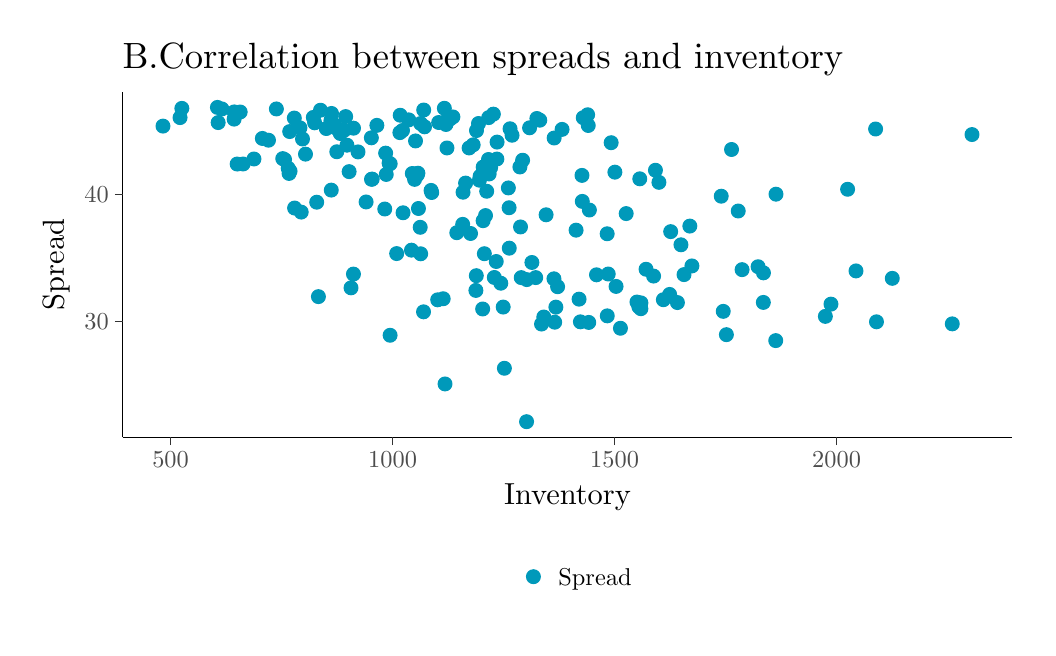
\begin{tikzpicture}[x=1pt,y=1pt]
\definecolor{fillColor}{RGB}{255,255,255}
\path[use as bounding box,fill=fillColor,fill opacity=0.00] (0,0) rectangle (361.35,216.81);
\begin{scope}
\path[clip] (  0.00,  0.00) rectangle (361.35,216.81);
\definecolor{drawColor}{RGB}{255,255,255}
\definecolor{fillColor}{RGB}{255,255,255}

\path[draw=drawColor,line width= 0.6pt,line join=round,line cap=round,fill=fillColor] (  0.00,  0.00) rectangle (361.35,216.81);
\end{scope}
\begin{scope}
\path[clip] ( 34.27, 68.75) rectangle (355.85,193.67);
\definecolor{fillColor}{RGB}{255,255,255}

\path[fill=fillColor] ( 34.27, 68.75) rectangle (355.85,193.67);
\definecolor{drawColor}{RGB}{0,153,186}
\definecolor{fillColor}{RGB}{0,153,186}

\path[draw=drawColor,line width= 0.4pt,line join=round,line cap=round,fill=fillColor] (150.81, 88.07) circle (  2.50);

\path[draw=drawColor,line width= 0.4pt,line join=round,line cap=round,fill=fillColor] (180.27, 74.43) circle (  2.50);

\path[draw=drawColor,line width= 0.4pt,line join=round,line cap=round,fill=fillColor] (172.26, 93.73) circle (  2.50);

\path[draw=drawColor,line width= 0.4pt,line join=round,line cap=round,fill=fillColor] (190.17,126.06) circle (  2.50);

\path[draw=drawColor,line width= 0.4pt,line join=round,line cap=round,fill=fillColor] (237.17,127.58) circle (  2.50);

\path[draw=drawColor,line width= 0.4pt,line join=round,line cap=round,fill=fillColor] (178.09,144.80) circle (  2.50);

\path[draw=drawColor,line width= 0.4pt,line join=round,line cap=round,fill=fillColor] (232.35,143.11) circle (  2.50);

\path[draw=drawColor,line width= 0.4pt,line join=round,line cap=round,fill=fillColor] (133.33,135.18) circle (  2.50);

\path[draw=drawColor,line width= 0.4pt,line join=round,line cap=round,fill=fillColor] (226.84,165.29) circle (  2.50);

\path[draw=drawColor,line width= 0.4pt,line join=round,line cap=round,fill=fillColor] (158.24,160.65) circle (  2.50);

\path[draw=drawColor,line width= 0.4pt,line join=round,line cap=round,fill=fillColor] (145.76,158.00) circle (  2.50);

\path[draw=drawColor,line width= 0.4pt,line join=round,line cap=round,fill=fillColor] (254.34,172.79) circle (  2.50);

\path[draw=drawColor,line width= 0.4pt,line join=round,line cap=round,fill=fillColor] ( 92.82,169.16) circle (  2.50);

\path[draw=drawColor,line width= 0.4pt,line join=round,line cap=round,fill=fillColor] (139.81,161.99) circle (  2.50);

\path[draw=drawColor,line width= 0.4pt,line join=round,line cap=round,fill=fillColor] (157.32,157.35) circle (  2.50);

\path[draw=drawColor,line width= 0.4pt,line join=round,line cap=round,fill=fillColor] (116.16,164.79) circle (  2.50);

\path[draw=drawColor,line width= 0.4pt,line join=round,line cap=round,fill=fillColor] (135.64,149.92) circle (  2.50);

\path[draw=drawColor,line width= 0.4pt,line join=round,line cap=round,fill=fillColor] (124.50,162.09) circle (  2.50);

\path[draw=drawColor,line width= 0.4pt,line join=round,line cap=round,fill=fillColor] (138.99,164.12) circle (  2.50);

\path[draw=drawColor,line width= 0.4pt,line join=round,line cap=round,fill=fillColor] (140.78,163.59) circle (  2.50);

\path[draw=drawColor,line width= 0.4pt,line join=round,line cap=round,fill=fillColor] ( 98.85,150.17) circle (  2.50);

\path[draw=drawColor,line width= 0.4pt,line join=round,line cap=round,fill=fillColor] ( 99.31,176.58) circle (  2.50);

\path[draw=drawColor,line width= 0.4pt,line join=round,line cap=round,fill=fillColor] (111.78,180.29) circle (  2.50);

\path[draw=drawColor,line width= 0.4pt,line join=round,line cap=round,fill=fillColor] (174.30,180.28) circle (  2.50);

\path[draw=drawColor,line width= 0.4pt,line join=round,line cap=round,fill=fillColor] (162.18,179.63) circle (  2.50);

\path[draw=drawColor,line width= 0.4pt,line join=round,line cap=round,fill=fillColor] (148.51,182.54) circle (  2.50);

\path[draw=drawColor,line width= 0.4pt,line join=round,line cap=round,fill=fillColor] (166.59,184.31) circle (  2.50);

\path[draw=drawColor,line width= 0.4pt,line join=round,line cap=round,fill=fillColor] (152.53,183.73) circle (  2.50);

\path[draw=drawColor,line width= 0.4pt,line join=round,line cap=round,fill=fillColor] (185.05,183.38) circle (  2.50);

\path[draw=drawColor,line width= 0.4pt,line join=round,line cap=round,fill=fillColor] (115.37,174.34) circle (  2.50);

\path[draw=drawColor,line width= 0.4pt,line join=round,line cap=round,fill=fillColor] (153.66,184.55) circle (  2.50);

\path[draw=drawColor,line width= 0.4pt,line join=round,line cap=round,fill=fillColor] (184.00,184.00) circle (  2.50);

\path[draw=drawColor,line width= 0.4pt,line join=round,line cap=round,fill=fillColor] (143.10,187.05) circle (  2.50);

\path[draw=drawColor,line width= 0.4pt,line join=round,line cap=round,fill=fillColor] (202.35,185.34) circle (  2.50);

\path[draw=drawColor,line width= 0.4pt,line join=round,line cap=round,fill=fillColor] (129.35,171.48) circle (  2.50);

\path[draw=drawColor,line width= 0.4pt,line join=round,line cap=round,fill=fillColor] (143.40,180.98) circle (  2.50);

\path[draw=drawColor,line width= 0.4pt,line join=round,line cap=round,fill=fillColor] (117.74,180.49) circle (  2.50);

\path[draw=drawColor,line width= 0.4pt,line join=round,line cap=round,fill=fillColor] (181.36,180.63) circle (  2.50);

\path[draw=drawColor,line width= 0.4pt,line join=round,line cap=round,fill=fillColor] (193.10,180.05) circle (  2.50);

\path[draw=drawColor,line width= 0.4pt,line join=round,line cap=round,fill=fillColor] (140.15,175.88) circle (  2.50);

\path[draw=drawColor,line width= 0.4pt,line join=round,line cap=round,fill=fillColor] (210.84,175.24) circle (  2.50);

\path[draw=drawColor,line width= 0.4pt,line join=round,line cap=round,fill=fillColor] (190.24,176.94) circle (  2.50);

\path[draw=drawColor,line width= 0.4pt,line join=round,line cap=round,fill=fillColor] (202.56,181.46) circle (  2.50);

\path[draw=drawColor,line width= 0.4pt,line join=round,line cap=round,fill=fillColor] (306.39,180.19) circle (  2.50);

\path[draw=drawColor,line width= 0.4pt,line join=round,line cap=round,fill=fillColor] (341.23,178.19) circle (  2.50);

\path[draw=drawColor,line width= 0.4pt,line join=round,line cap=round,fill=fillColor] (178.84,168.91) circle (  2.50);

\path[draw=drawColor,line width= 0.4pt,line join=round,line cap=round,fill=fillColor] (166.53,167.39) circle (  2.50);

\path[draw=drawColor,line width= 0.4pt,line join=round,line cap=round,fill=fillColor] (159.51,173.34) circle (  2.50);

\path[draw=drawColor,line width= 0.4pt,line join=round,line cap=round,fill=fillColor] (166.75,163.95) circle (  2.50);

\path[draw=drawColor,line width= 0.4pt,line join=round,line cap=round,fill=fillColor] (212.19,164.60) circle (  2.50);

\path[draw=drawColor,line width= 0.4pt,line join=round,line cap=round,fill=fillColor] (221.18,162.19) circle (  2.50);

\path[draw=drawColor,line width= 0.4pt,line join=round,line cap=round,fill=fillColor] (202.97,150.92) circle (  2.50);

\path[draw=drawColor,line width= 0.4pt,line join=round,line cap=round,fill=fillColor] (239.27,145.11) circle (  2.50);

\path[draw=drawColor,line width= 0.4pt,line join=round,line cap=round,fill=fillColor] (155.06,142.72) circle (  2.50);

\path[draw=drawColor,line width= 0.4pt,line join=round,line cap=round,fill=fillColor] (199.25,118.71) circle (  2.50);

\path[draw=drawColor,line width= 0.4pt,line join=round,line cap=round,fill=fillColor] (226.17,127.05) circle (  2.50);

\path[draw=drawColor,line width= 0.4pt,line join=round,line cap=round,fill=fillColor] (221.58,115.26) circle (  2.50);

\path[draw=drawColor,line width= 0.4pt,line join=round,line cap=round,fill=fillColor] (312.42,126.23) circle (  2.50);

\path[draw=drawColor,line width= 0.4pt,line join=round,line cap=round,fill=fillColor] (169.31,132.31) circle (  2.50);

\path[draw=drawColor,line width= 0.4pt,line join=round,line cap=round,fill=fillColor] (265.87,128.21) circle (  2.50);

\path[draw=drawColor,line width= 0.4pt,line join=round,line cap=round,fill=fillColor] (162.11,127.19) circle (  2.50);

\path[draw=drawColor,line width= 0.4pt,line join=round,line cap=round,fill=fillColor] (209.79,127.79) circle (  2.50);

\path[draw=drawColor,line width= 0.4pt,line join=round,line cap=round,fill=fillColor] (263.93,130.43) circle (  2.50);

\path[draw=drawColor,line width= 0.4pt,line join=round,line cap=round,fill=fillColor] (299.31,128.91) circle (  2.50);

\path[draw=drawColor,line width= 0.4pt,line join=round,line cap=round,fill=fillColor] (198.17,143.64) circle (  2.50);

\path[draw=drawColor,line width= 0.4pt,line join=round,line cap=round,fill=fillColor] (138.69,136.41) circle (  2.50);

\path[draw=drawColor,line width= 0.4pt,line join=round,line cap=round,fill=fillColor] (160.03,142.44) circle (  2.50);

\path[draw=drawColor,line width= 0.4pt,line join=round,line cap=round,fill=fillColor] (164.57,147.06) circle (  2.50);

\path[draw=drawColor,line width= 0.4pt,line join=round,line cap=round,fill=fillColor] (129.03,151.28) circle (  2.50);

\path[draw=drawColor,line width= 0.4pt,line join=round,line cap=round,fill=fillColor] (200.41,154.03) circle (  2.50);

\path[draw=drawColor,line width= 0.4pt,line join=round,line cap=round,fill=fillColor] (240.02,130.71) circle (  2.50);

\path[draw=drawColor,line width= 0.4pt,line join=round,line cap=round,fill=fillColor] (130.96,105.66) circle (  2.50);

\path[draw=drawColor,line width= 0.4pt,line join=round,line cap=round,fill=fillColor] (290.27,116.91) circle (  2.50);

\path[draw=drawColor,line width= 0.4pt,line join=round,line cap=round,fill=fillColor] (231.97,120.41) circle (  2.50);

\path[draw=drawColor,line width= 0.4pt,line join=round,line cap=round,fill=fillColor] (164.41,115.16) circle (  2.50);

\path[draw=drawColor,line width= 0.4pt,line join=round,line cap=round,fill=fillColor] (212.61,123.31) circle (  2.50);

\path[draw=drawColor,line width= 0.4pt,line join=round,line cap=round,fill=fillColor] (191.49,123.20) circle (  2.50);

\path[draw=drawColor,line width= 0.4pt,line join=round,line cap=round,fill=fillColor] (220.86,115.93) circle (  2.50);

\path[draw=drawColor,line width= 0.4pt,line join=round,line cap=round,fill=fillColor] (214.20,108.19) circle (  2.50);

\path[draw=drawColor,line width= 0.4pt,line join=round,line cap=round,fill=fillColor] (199.73,110.52) circle (  2.50);

\path[draw=drawColor,line width= 0.4pt,line join=round,line cap=round,fill=fillColor] (270.40,156.64) circle (  2.50);

\path[draw=drawColor,line width= 0.4pt,line join=round,line cap=round,fill=fillColor] (250.61,155.91) circle (  2.50);

\path[draw=drawColor,line width= 0.4pt,line join=round,line cap=round,fill=fillColor] (146.00,157.24) circle (  2.50);

\path[draw=drawColor,line width= 0.4pt,line join=round,line cap=round,fill=fillColor] (167.28,166.21) circle (  2.50);

\path[draw=drawColor,line width= 0.4pt,line join=round,line cap=round,fill=fillColor] ( 94.68,179.27) circle (  2.50);

\path[draw=drawColor,line width= 0.4pt,line join=round,line cap=round,fill=fillColor] (135.44,179.65) circle (  2.50);

\path[draw=drawColor,line width= 0.4pt,line join=round,line cap=round,fill=fillColor] (107.90,180.36) circle (  2.50);

\path[draw=drawColor,line width= 0.4pt,line join=round,line cap=round,fill=fillColor] (151.55,183.36) circle (  2.50);

\path[draw=drawColor,line width= 0.4pt,line join=round,line cap=round,fill=fillColor] (162.91,182.18) circle (  2.50);

\path[draw=drawColor,line width= 0.4pt,line join=round,line cap=round,fill=fillColor] (137.70,183.49) circle (  2.50);

\path[draw=drawColor,line width= 0.4pt,line join=round,line cap=round,fill=fillColor] ( 89.87,187.44) circle (  2.50);

\path[draw=drawColor,line width= 0.4pt,line join=round,line cap=round,fill=fillColor] ( 87.02,176.15) circle (  2.50);

\path[draw=drawColor,line width= 0.4pt,line join=round,line cap=round,fill=fillColor] ( 76.79,186.34) circle (  2.50);

\path[draw=drawColor,line width= 0.4pt,line join=round,line cap=round,fill=fillColor] ( 55.71,187.65) circle (  2.50);

\path[draw=drawColor,line width= 0.4pt,line join=round,line cap=round,fill=fillColor] ( 70.18,187.44) circle (  2.50);

\path[draw=drawColor,line width= 0.4pt,line join=round,line cap=round,fill=fillColor] ( 68.57,188.00) circle (  2.50);

\path[draw=drawColor,line width= 0.4pt,line join=round,line cap=round,fill=fillColor] ( 68.83,182.52) circle (  2.50);

\path[draw=drawColor,line width= 0.4pt,line join=round,line cap=round,fill=fillColor] (111.70,171.97) circle (  2.50);

\path[draw=drawColor,line width= 0.4pt,line join=round,line cap=round,fill=fillColor] ( 48.89,181.24) circle (  2.50);

\path[draw=drawColor,line width= 0.4pt,line join=round,line cap=round,fill=fillColor] (100.39,171.11) circle (  2.50);

\path[draw=drawColor,line width= 0.4pt,line join=round,line cap=round,fill=fillColor] ( 75.69,167.53) circle (  2.50);

\path[draw=drawColor,line width= 0.4pt,line join=round,line cap=round,fill=fillColor] ( 81.77,169.36) circle (  2.50);

\path[draw=drawColor,line width= 0.4pt,line join=round,line cap=round,fill=fillColor] (104.44,153.74) circle (  2.50);

\path[draw=drawColor,line width= 0.4pt,line join=round,line cap=round,fill=fillColor] ( 96.45,151.63) circle (  2.50);

\path[draw=drawColor,line width= 0.4pt,line join=round,line cap=round,fill=fillColor] ( 94.45,164.13) circle (  2.50);

\path[draw=drawColor,line width= 0.4pt,line join=round,line cap=round,fill=fillColor] (129.57,163.78) circle (  2.50);

\path[draw=drawColor,line width= 0.4pt,line join=round,line cap=round,fill=fillColor] (124.24,162.02) circle (  2.50);

\path[draw=drawColor,line width= 0.4pt,line join=round,line cap=round,fill=fillColor] (163.24,161.69) circle (  2.50);

\path[draw=drawColor,line width= 0.4pt,line join=round,line cap=round,fill=fillColor] (109.70,158.11) circle (  2.50);

\path[draw=drawColor,line width= 0.4pt,line join=round,line cap=round,fill=fillColor] (177.87,166.47) circle (  2.50);

\path[draw=drawColor,line width= 0.4pt,line join=round,line cap=round,fill=fillColor] (164.59,166.43) circle (  2.50);

\path[draw=drawColor,line width= 0.4pt,line join=round,line cap=round,fill=fillColor] ( 94.13,166.03) circle (  2.50);

\path[draw=drawColor,line width= 0.4pt,line join=round,line cap=round,fill=fillColor] (130.59,167.84) circle (  2.50);

\path[draw=drawColor,line width= 0.4pt,line join=round,line cap=round,fill=fillColor] ( 84.80,176.78) circle (  2.50);

\path[draw=drawColor,line width= 0.4pt,line join=round,line cap=round,fill=fillColor] ( 77.84,167.55) circle (  2.50);

\path[draw=drawColor,line width= 0.4pt,line join=round,line cap=round,fill=fillColor] (109.58,183.34) circle (  2.50);

\path[draw=drawColor,line width= 0.4pt,line join=round,line cap=round,fill=fillColor] ( 74.97,185.60) circle (  2.50);

\path[draw=drawColor,line width= 0.4pt,line join=round,line cap=round,fill=fillColor] ( 92.17,169.49) circle (  2.50);

\path[draw=drawColor,line width= 0.4pt,line join=round,line cap=round,fill=fillColor] (168.28,185.57) circle (  2.50);

\path[draw=drawColor,line width= 0.4pt,line join=round,line cap=round,fill=fillColor] (114.91,184.68) circle (  2.50);

\path[draw=drawColor,line width= 0.4pt,line join=round,line cap=round,fill=fillColor] ( 96.35,184.15) circle (  2.50);

\path[draw=drawColor,line width= 0.4pt,line join=round,line cap=round,fill=fillColor] (110.99,181.50) circle (  2.50);

\path[draw=drawColor,line width= 0.4pt,line join=round,line cap=round,fill=fillColor] (175.03,177.94) circle (  2.50);

\path[draw=drawColor,line width= 0.4pt,line join=round,line cap=round,fill=fillColor] (169.62,175.46) circle (  2.50);

\path[draw=drawColor,line width= 0.4pt,line join=round,line cap=round,fill=fillColor] (124.19,177.01) circle (  2.50);

\path[draw=drawColor,line width= 0.4pt,line join=round,line cap=round,fill=fillColor] (142.00,182.17) circle (  2.50);

\path[draw=drawColor,line width= 0.4pt,line join=round,line cap=round,fill=fillColor] ( 94.81,164.96) circle (  2.50);

\path[draw=drawColor,line width= 0.4pt,line join=round,line cap=round,fill=fillColor] (126.18,181.51) circle (  2.50);

\path[draw=drawColor,line width= 0.4pt,line join=round,line cap=round,fill=fillColor] (150.56,187.68) circle (  2.50);

\path[draw=drawColor,line width= 0.4pt,line join=round,line cap=round,fill=fillColor] ( 55.06,184.31) circle (  2.50);

\path[draw=drawColor,line width= 0.4pt,line join=round,line cap=round,fill=fillColor] ( 74.60,183.76) circle (  2.50);

\path[draw=drawColor,line width= 0.4pt,line join=round,line cap=round,fill=fillColor] (109.79,185.81) circle (  2.50);

\path[draw=drawColor,line width= 0.4pt,line join=round,line cap=round,fill=fillColor] ( 75.10,185.69) circle (  2.50);

\path[draw=drawColor,line width= 0.4pt,line join=round,line cap=round,fill=fillColor] (134.61,185.16) circle (  2.50);

\path[draw=drawColor,line width= 0.4pt,line join=round,line cap=round,fill=fillColor] (103.69,182.43) circle (  2.50);

\path[draw=drawColor,line width= 0.4pt,line join=round,line cap=round,fill=fillColor] ( 98.37,180.62) circle (  2.50);

\path[draw=drawColor,line width= 0.4pt,line join=round,line cap=round,fill=fillColor] (151.14,181.82) circle (  2.50);

\path[draw=drawColor,line width= 0.4pt,line join=round,line cap=round,fill=fillColor] (200.75,184.27) circle (  2.50);

\path[draw=drawColor,line width= 0.4pt,line join=round,line cap=round,fill=fillColor] (105.81,186.98) circle (  2.50);

\path[draw=drawColor,line width= 0.4pt,line join=round,line cap=round,fill=fillColor] ( 74.61,186.37) circle (  2.50);

\path[draw=drawColor,line width= 0.4pt,line join=round,line cap=round,fill=fillColor] (103.22,184.37) circle (  2.50);

\path[draw=drawColor,line width= 0.4pt,line join=round,line cap=round,fill=fillColor] (112.97,178.57) circle (  2.50);

\path[draw=drawColor,line width= 0.4pt,line join=round,line cap=round,fill=fillColor] (134.50,178.88) circle (  2.50);

\path[draw=drawColor,line width= 0.4pt,line join=round,line cap=round,fill=fillColor] (114.31,179.70) circle (  2.50);

\path[draw=drawColor,line width= 0.4pt,line join=round,line cap=round,fill=fillColor] (165.86,157.70) circle (  2.50);

\path[draw=drawColor,line width= 0.4pt,line join=round,line cap=round,fill=fillColor] (130.99,167.64) circle (  2.50);

\path[draw=drawColor,line width= 0.4pt,line join=round,line cap=round,fill=fillColor] (169.54,169.34) circle (  2.50);

\path[draw=drawColor,line width= 0.4pt,line join=round,line cap=round,fill=fillColor] (119.37,171.92) circle (  2.50);

\path[draw=drawColor,line width= 0.4pt,line join=round,line cap=round,fill=fillColor] (151.51,173.34) circle (  2.50);

\path[draw=drawColor,line width= 0.4pt,line join=round,line cap=round,fill=fillColor] (160.98,174.47) circle (  2.50);

\path[draw=drawColor,line width= 0.4pt,line join=round,line cap=round,fill=fillColor] (166.51,169.17) circle (  2.50);

\path[draw=drawColor,line width= 0.4pt,line join=round,line cap=round,fill=fillColor] (173.96,151.74) circle (  2.50);

\path[draw=drawColor,line width= 0.4pt,line join=round,line cap=round,fill=fillColor] (200.29,163.43) circle (  2.50);

\path[draw=drawColor,line width= 0.4pt,line join=round,line cap=round,fill=fillColor] (163.49,163.14) circle (  2.50);

\path[draw=drawColor,line width= 0.4pt,line join=round,line cap=round,fill=fillColor] (296.28,158.41) circle (  2.50);

\path[draw=drawColor,line width= 0.4pt,line join=round,line cap=round,fill=fillColor] (122.29,153.83) circle (  2.50);

\path[draw=drawColor,line width= 0.4pt,line join=round,line cap=round,fill=fillColor] (141.20,151.47) circle (  2.50);

\path[draw=drawColor,line width= 0.4pt,line join=round,line cap=round,fill=fillColor] (216.27,149.63) circle (  2.50);

\path[draw=drawColor,line width= 0.4pt,line join=round,line cap=round,fill=fillColor] (165.02,135.13) circle (  2.50);

\path[draw=drawColor,line width= 0.4pt,line join=round,line cap=round,fill=fillColor] (157.19,145.74) circle (  2.50);

\path[draw=drawColor,line width= 0.4pt,line join=round,line cap=round,fill=fillColor] (165.44,148.91) circle (  2.50);

\path[draw=drawColor,line width= 0.4pt,line join=round,line cap=round,fill=fillColor] (256.76,150.56) circle (  2.50);

\path[draw=drawColor,line width= 0.4pt,line join=round,line cap=round,fill=fillColor] (141.84,144.67) circle (  2.50);

\path[draw=drawColor,line width= 0.4pt,line join=round,line cap=round,fill=fillColor] (173.70,158.90) circle (  2.50);

\path[draw=drawColor,line width= 0.4pt,line join=round,line cap=round,fill=fillColor] (228.10,160.92) circle (  2.50);

\path[draw=drawColor,line width= 0.4pt,line join=round,line cap=round,fill=fillColor] (141.01,164.22) circle (  2.50);

\path[draw=drawColor,line width= 0.4pt,line join=round,line cap=round,fill=fillColor] (187.33,149.19) circle (  2.50);

\path[draw=drawColor,line width= 0.4pt,line join=round,line cap=round,fill=fillColor] (142.01,135.10) circle (  2.50);

\path[draw=drawColor,line width= 0.4pt,line join=round,line cap=round,fill=fillColor] (209.40,142.33) circle (  2.50);

\path[draw=drawColor,line width= 0.4pt,line join=round,line cap=round,fill=fillColor] (182.20,131.96) circle (  2.50);

\path[draw=drawColor,line width= 0.4pt,line join=round,line cap=round,fill=fillColor] (170.96,124.47) circle (  2.50);

\path[draw=drawColor,line width= 0.4pt,line join=round,line cap=round,fill=fillColor] (236.06,138.35) circle (  2.50);

\path[draw=drawColor,line width= 0.4pt,line join=round,line cap=round,fill=fillColor] (174.02,137.13) circle (  2.50);

\path[draw=drawColor,line width= 0.4pt,line join=round,line cap=round,fill=fillColor] (223.45,129.51) circle (  2.50);

\path[draw=drawColor,line width= 0.4pt,line join=round,line cap=round,fill=fillColor] (116.84,122.80) circle (  2.50);

\path[draw=drawColor,line width= 0.4pt,line join=round,line cap=round,fill=fillColor] (258.15,129.37) circle (  2.50);

\path[draw=drawColor,line width= 0.4pt,line join=round,line cap=round,fill=fillColor] (205.54,127.50) circle (  2.50);

\path[draw=drawColor,line width= 0.4pt,line join=round,line cap=round,fill=fillColor] (168.62,126.54) circle (  2.50);

\path[draw=drawColor,line width= 0.4pt,line join=round,line cap=round,fill=fillColor] (117.72,127.77) circle (  2.50);

\path[draw=drawColor,line width= 0.4pt,line join=round,line cap=round,fill=fillColor] (180.34,125.78) circle (  2.50);

\path[draw=drawColor,line width= 0.4pt,line join=round,line cap=round,fill=fillColor] (183.58,126.50) circle (  2.50);

\path[draw=drawColor,line width= 0.4pt,line join=round,line cap=round,fill=fillColor] (178.35,126.49) circle (  2.50);

\path[draw=drawColor,line width= 0.4pt,line join=round,line cap=round,fill=fillColor] (161.96,121.86) circle (  2.50);

\path[draw=drawColor,line width= 0.4pt,line join=round,line cap=round,fill=fillColor] (234.78,117.48) circle (  2.50);

\path[draw=drawColor,line width= 0.4pt,line join=round,line cap=round,fill=fillColor] (148.16,118.47) circle (  2.50);

\path[draw=drawColor,line width= 0.4pt,line join=round,line cap=round,fill=fillColor] (229.70,118.50) circle (  2.50);

\path[draw=drawColor,line width= 0.4pt,line join=round,line cap=round,fill=fillColor] (221.60,117.36) circle (  2.50);

\path[draw=drawColor,line width= 0.4pt,line join=round,line cap=round,fill=fillColor] (190.86,115.82) circle (  2.50);

\path[draw=drawColor,line width= 0.4pt,line join=round,line cap=round,fill=fillColor] (171.83,115.85) circle (  2.50);

\path[draw=drawColor,line width= 0.4pt,line join=round,line cap=round,fill=fillColor] (288.24,112.48) circle (  2.50);

\path[draw=drawColor,line width= 0.4pt,line join=round,line cap=round,fill=fillColor] (270.31,103.73) circle (  2.50);

\path[draw=drawColor,line width= 0.4pt,line join=round,line cap=round,fill=fillColor] (143.04,114.13) circle (  2.50);

\path[draw=drawColor,line width= 0.4pt,line join=round,line cap=round,fill=fillColor] (306.71,110.52) circle (  2.50);

\path[draw=drawColor,line width= 0.4pt,line join=round,line cap=round,fill=fillColor] (334.10,109.78) circle (  2.50);

\path[draw=drawColor,line width= 0.4pt,line join=round,line cap=round,fill=fillColor] (185.68,109.71) circle (  2.50);

\path[draw=drawColor,line width= 0.4pt,line join=round,line cap=round,fill=fillColor] (190.44,110.38) circle (  2.50);

\path[draw=drawColor,line width= 0.4pt,line join=round,line cap=round,fill=fillColor] (252.48,105.88) circle (  2.50);

\path[draw=drawColor,line width= 0.4pt,line join=round,line cap=round,fill=fillColor] (202.74,110.30) circle (  2.50);

\path[draw=drawColor,line width= 0.4pt,line join=round,line cap=round,fill=fillColor] (186.50,112.26) circle (  2.50);

\path[draw=drawColor,line width= 0.4pt,line join=round,line cap=round,fill=fillColor] (251.34,114.30) circle (  2.50);

\path[draw=drawColor,line width= 0.4pt,line join=round,line cap=round,fill=fillColor] (209.44,112.67) circle (  2.50);

\path[draw=drawColor,line width= 0.4pt,line join=round,line cap=round,fill=fillColor] (105.06,119.62) circle (  2.50);

\path[draw=drawColor,line width= 0.4pt,line join=round,line cap=round,fill=fillColor] (150.15,118.86) circle (  2.50);

\path[draw=drawColor,line width= 0.4pt,line join=round,line cap=round,fill=fillColor] (265.83,117.53) circle (  2.50);

\path[draw=drawColor,line width= 0.4pt,line join=round,line cap=round,fill=fillColor] (220.16,117.67) circle (  2.50);
\end{scope}
\begin{scope}
\path[clip] (  0.00,  0.00) rectangle (361.35,216.81);
\definecolor{drawColor}{RGB}{0,0,0}

\path[draw=drawColor,line width= 0.6pt,line join=round] ( 34.27, 68.75) --
	( 34.27,193.67);
\end{scope}
\begin{scope}
\path[clip] (  0.00,  0.00) rectangle (361.35,216.81);
\definecolor{drawColor}{gray}{0.30}

\node[text=drawColor,anchor=base east,inner sep=0pt, outer sep=0pt, scale=  0.88] at ( 29.32,107.59) {30};

\node[text=drawColor,anchor=base east,inner sep=0pt, outer sep=0pt, scale=  0.88] at ( 29.32,153.46) {40};
\end{scope}
\begin{scope}
\path[clip] (  0.00,  0.00) rectangle (361.35,216.81);
\definecolor{drawColor}{gray}{0.20}

\path[draw=drawColor,line width= 0.6pt,line join=round] ( 31.52,110.62) --
	( 34.27,110.62);

\path[draw=drawColor,line width= 0.6pt,line join=round] ( 31.52,156.49) --
	( 34.27,156.49);
\end{scope}
\begin{scope}
\path[clip] (  0.00,  0.00) rectangle (361.35,216.81);
\definecolor{drawColor}{RGB}{0,0,0}

\path[draw=drawColor,line width= 0.6pt,line join=round] ( 34.27, 68.75) --
	(355.85, 68.75);
\end{scope}
\begin{scope}
\path[clip] (  0.00,  0.00) rectangle (361.35,216.81);
\definecolor{drawColor}{gray}{0.20}

\path[draw=drawColor,line width= 0.6pt,line join=round] ( 51.64, 66.00) --
	( 51.64, 68.75);

\path[draw=drawColor,line width= 0.6pt,line join=round] (131.86, 66.00) --
	(131.86, 68.75);

\path[draw=drawColor,line width= 0.6pt,line join=round] (212.08, 66.00) --
	(212.08, 68.75);

\path[draw=drawColor,line width= 0.6pt,line join=round] (292.30, 66.00) --
	(292.30, 68.75);
\end{scope}
\begin{scope}
\path[clip] (  0.00,  0.00) rectangle (361.35,216.81);
\definecolor{drawColor}{gray}{0.30}

\node[text=drawColor,anchor=base,inner sep=0pt, outer sep=0pt, scale=  0.88] at ( 51.64, 57.74) {500};

\node[text=drawColor,anchor=base,inner sep=0pt, outer sep=0pt, scale=  0.88] at (131.86, 57.74) {1000};

\node[text=drawColor,anchor=base,inner sep=0pt, outer sep=0pt, scale=  0.88] at (212.08, 57.74) {1500};

\node[text=drawColor,anchor=base,inner sep=0pt, outer sep=0pt, scale=  0.88] at (292.30, 57.74) {2000};
\end{scope}
\begin{scope}
\path[clip] (  0.00,  0.00) rectangle (361.35,216.81);
\definecolor{drawColor}{RGB}{0,0,0}

\node[text=drawColor,anchor=base,inner sep=0pt, outer sep=0pt, scale=  1.10] at (195.06, 44.66) {Inventory};
\end{scope}
\begin{scope}
\path[clip] (  0.00,  0.00) rectangle (361.35,216.81);
\definecolor{drawColor}{RGB}{0,0,0}

\node[text=drawColor,rotate= 90.00,anchor=base,inner sep=0pt, outer sep=0pt, scale=  1.10] at ( 13.08,131.21) {Spread};
\end{scope}
\begin{scope}
\path[clip] (  0.00,  0.00) rectangle (361.35,216.81);
\definecolor{fillColor}{RGB}{255,255,255}

\path[fill=fillColor] (166.22,  5.50) rectangle (223.90, 31.34);
\end{scope}
\begin{scope}
\path[clip] (  0.00,  0.00) rectangle (361.35,216.81);
\definecolor{drawColor}{RGB}{0,153,186}
\definecolor{fillColor}{RGB}{0,153,186}

\path[draw=drawColor,line width= 0.4pt,line join=round,line cap=round,fill=fillColor] (182.75, 18.42) circle (  2.50);
\end{scope}
\begin{scope}
\path[clip] (  0.00,  0.00) rectangle (361.35,216.81);
\definecolor{drawColor}{RGB}{0,0,0}

\node[text=drawColor,anchor=base west,inner sep=0pt, outer sep=0pt, scale=  0.88] at (191.79, 15.39) {Spread};
\end{scope}
\begin{scope}
\path[clip] (  0.00,  0.00) rectangle (361.35,216.81);
\definecolor{drawColor}{RGB}{0,0,0}

\node[text=drawColor,anchor=base west,inner sep=0pt, outer sep=0pt, scale=  1.32] at ( 34.27,202.22) {B.Correlation between spreads and inventory};
\end{scope}
\end{tikzpicture}

    		%Captions and Labels can be used since this is a figure environment
    		\caption{ \small Correlation between spreads and inventory for DealerMarket-v2.}
    		\label{fig:dmv12}
    \end{figure}
  
\end{frame}

\subsection{Demo}

\begin{frame}
  \frametitle{\hfill Demo 1 - Incompetent Dealer agent 84 episodes}
  
  \centering
  \includemedia[width=0.5\linewidth,
  height=0.5\linewidth,
  activate=pageopen,
  passcontext,
  transparent, 
  addresource=dmv1ic.mp4,
flashvars={source=dmv1ic.mp4}
]{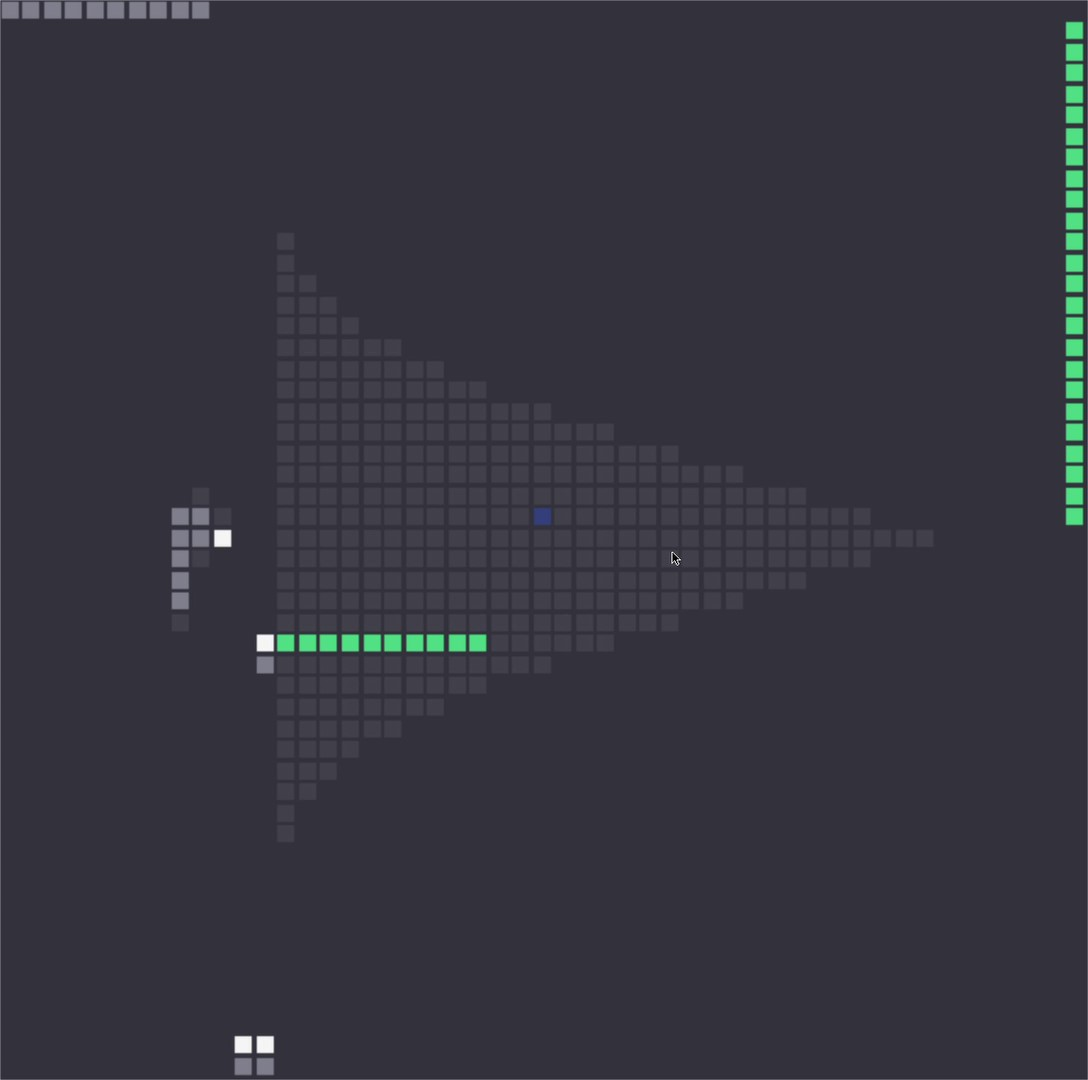
\includegraphics[width=0.6\linewidth]{best_84eps.jpg}}{VPlayer.swf}
  
\end{frame}

\begin{frame}
  \frametitle{\hfill Demo 2 - More Competent Dealer agent 1169 episodes}
  
  \centering
  \includemedia[width=0.5\linewidth,
  height=0.5\linewidth,
  activate=pageopen,
  passcontext,
  transparent, 
  addresource=dmv1lc.mp4,
flashvars={source=dmv1lc.mp4}
]{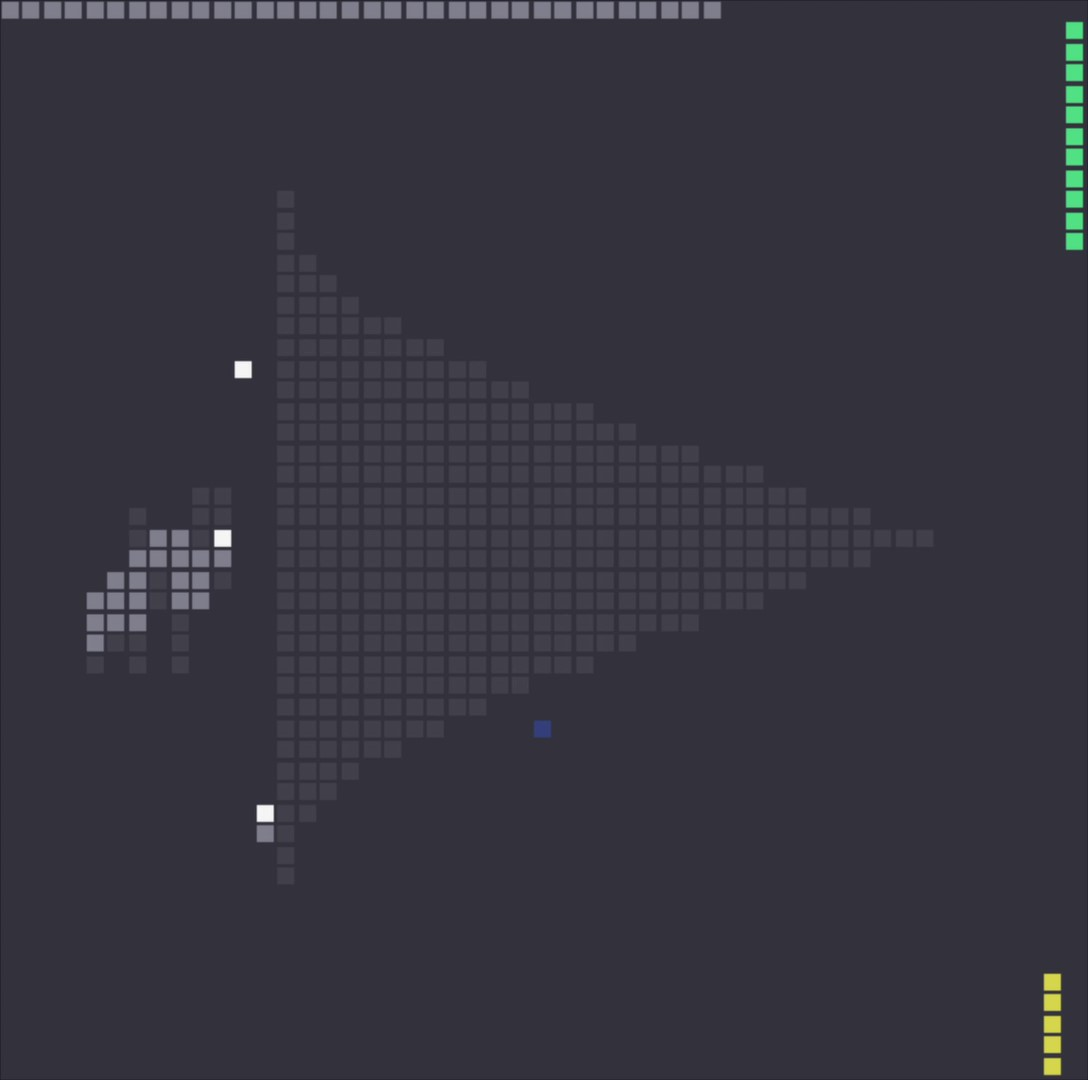
\includegraphics[width=0.6\linewidth]{best_1169eps.jpg}}{VPlayer.swf}
  
\end{frame}

\begin{frame}
  \frametitle{\hfill Demo 3 - Best Dealer agent 2006 episodes}
  
  \centering
  \includemedia[width=0.5\linewidth,
  height=0.5\linewidth,
  activate=pageopen,
  passcontext,
  transparent, 
  addresource=dmv1best.mp4,
flashvars={source=dmv1best.mp4}
]{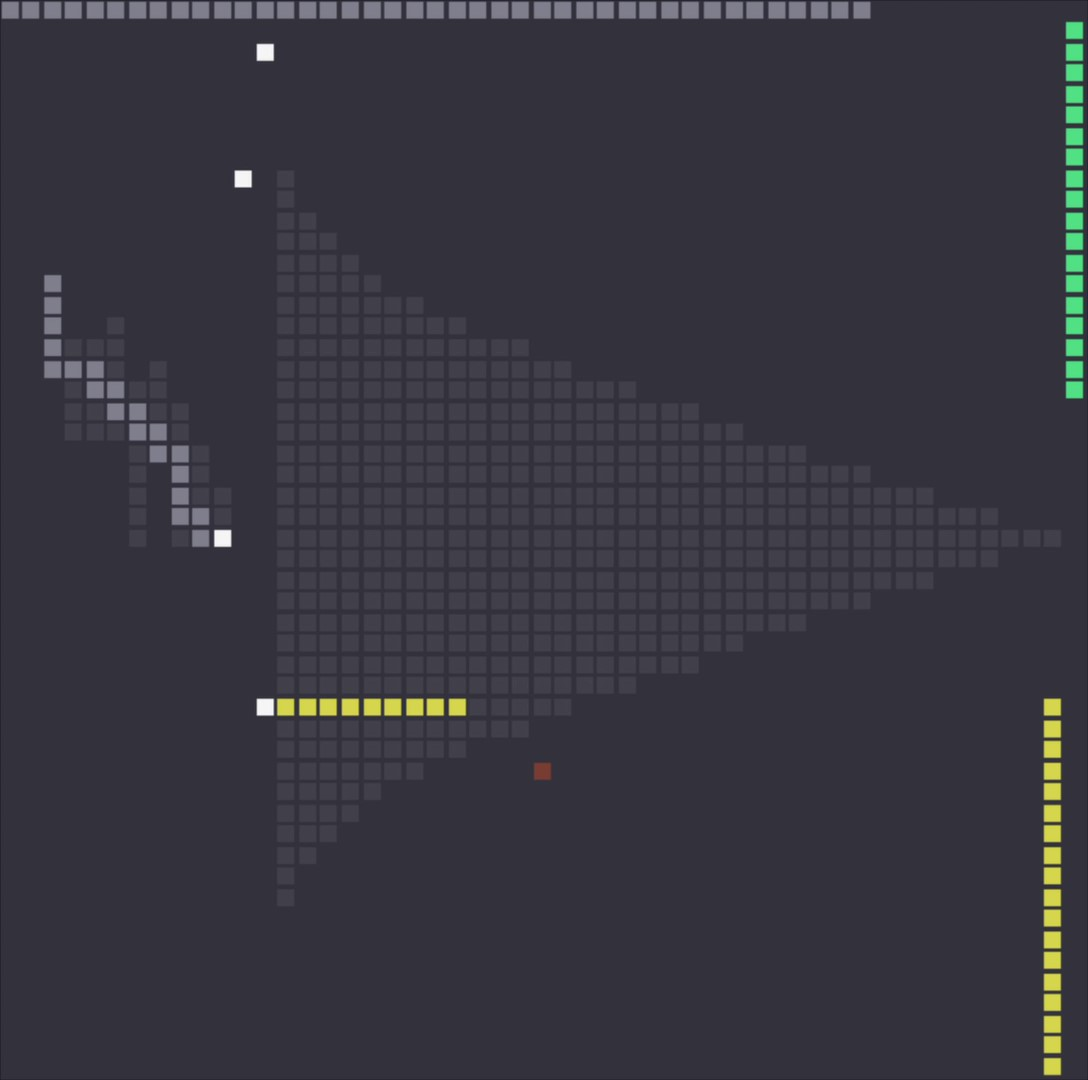
\includegraphics[width=0.6\linewidth]{best_2006eps.jpg}}{VPlayer.swf}
  
\end{frame}

\begin{frame}
  \frametitle{\hfill Demo 4 - Incompetent LOB agent 20 episodes}
  
  \centering
  \includemedia[width=0.5\linewidth,
  height=0.5\linewidth,
  activate=pageopen,
  passcontext,
  transparent, 
  addresource=lobv1ic.mp4,
flashvars={source=lobv1ic.mp4}
]{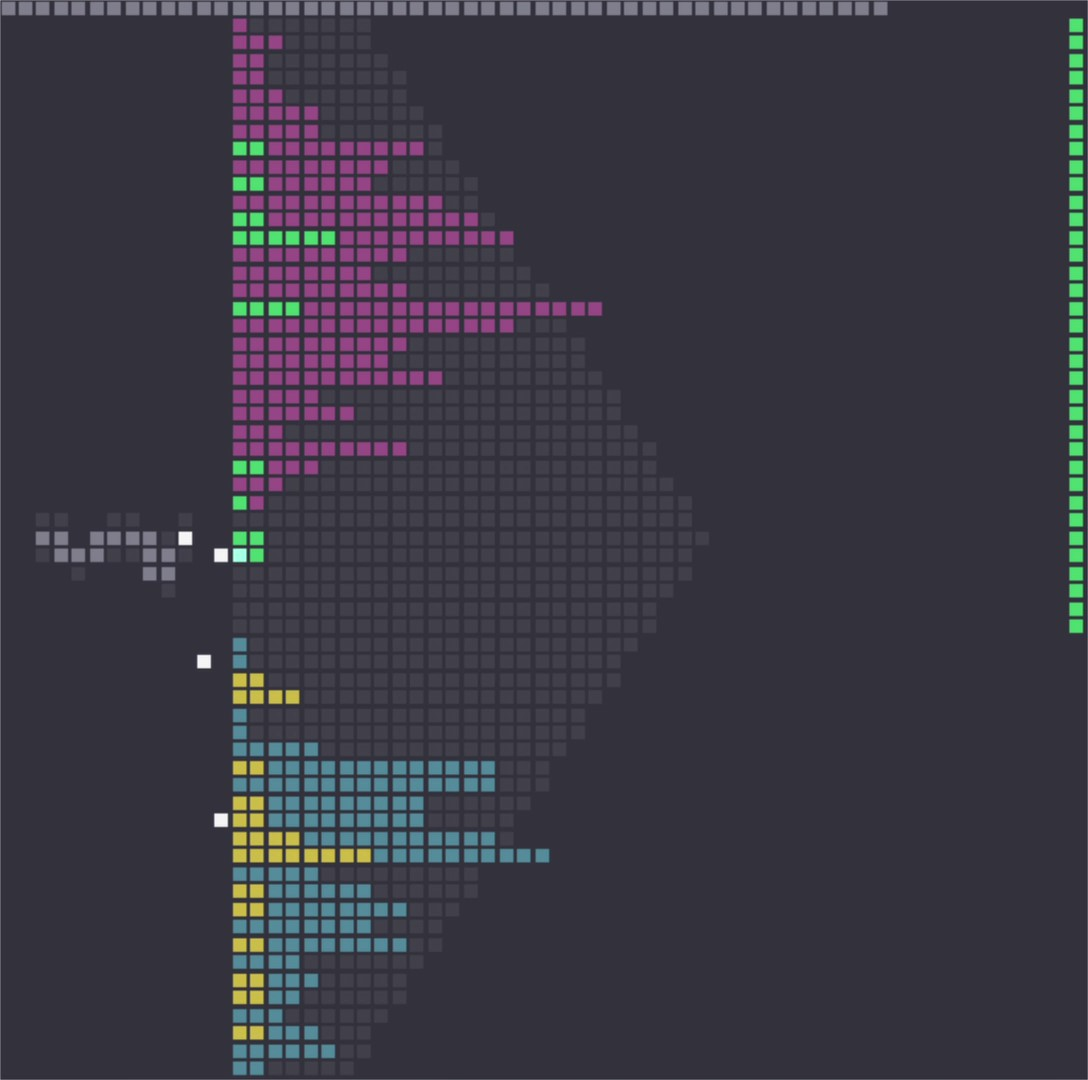
\includegraphics[width=0.6\linewidth]{LOBMarket_eps1_lstm.jpg}}{VPlayer.swf}
  
\end{frame}

\begin{frame}
  \frametitle{\hfill Demo 5 - Best LOB agent 1869 episodes}
  
  \centering
  \includemedia[width=0.5\linewidth,
  height=0.5\linewidth,
  activate=pageopen,
  passcontext,
  transparent, 
  addresource=lobv1best.mp4,
flashvars={source=lobv1best.mp4}
]{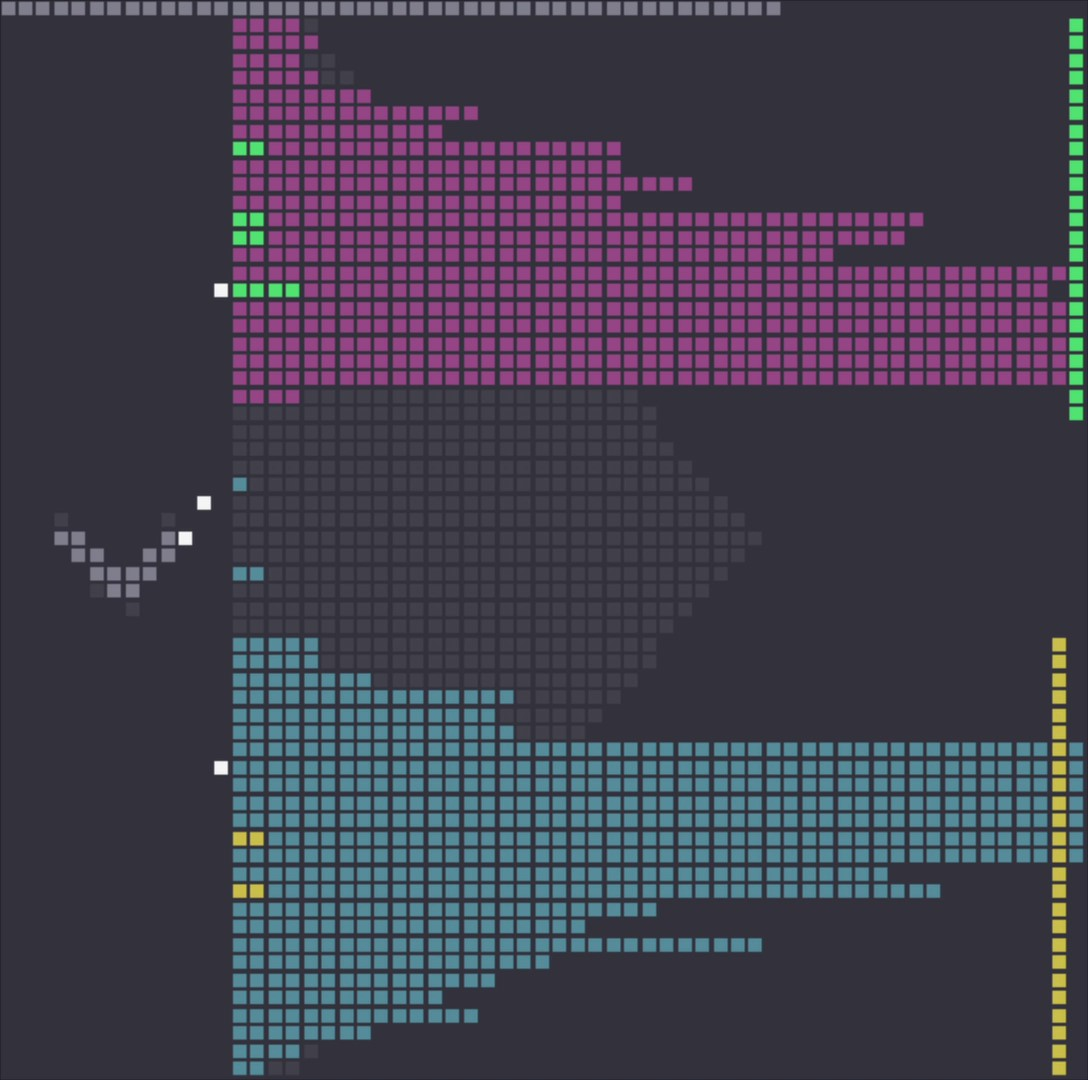
\includegraphics[width=0.6\linewidth]{LOBMarket_eps1132_lstm.jpg}}{VPlayer.swf}
  
\end{frame}


%%%%%%%%%%%%%%%%%%%%%%%%%%%%%%%%%%%%%%%%%%%%%%%%%%%%%%%%%%%%
% Discussion, Analysis & Future studies
%%%%%%%%%%%%%%%%%%%%%%%%%%%%%%%%%%%%%%%%%%%%%%%%%%%%%%%%%%%% 
\section{Discussion, Conclusions \& Future Work}

\begin{frame}
  \frametitle{\hfill Discussion, Conclusions \& Future Work}
\textit{"Everything has to come to an end, sometime"} - \\   \textbf{L. Frank Baum, The Marvelous Land of Oz}
  \begin{columns}[t]
    \column{.4\textwidth}
    \begin{block}{Conclusions}
    \begin{itemize}
        \item Realistic simulations
        \item DQN \& PPO agents can replicate known trading dynamics
        \item Reinforcement Learning is suitable for Market Microstructure simulations
    \end{itemize}
    \end{block}
    
    \column{.4\textwidth}
    \begin{block}{Future Work}
    \begin{itemize}
        \item Look at multiagent framework with competitive self-play
        \item Test other market structures i.e. Derivatives market
        \item Train agents on real world historical data
    \end{itemize}
    \end{block}
\end{columns}

\end{frame}

%%%%%%%%%%%%%%%%%%%%%%%%%%%%%%%%%%%%%%%%%%%%%%%%%%%%%%%%%%%%
% References
%%%%%%%%%%%%%%%%%%%%%%%%%%%%%%%%%%%%%%%%%%%%%%%%%%%%%%%%%%%% 
\section{References}

\begin{frame}[shrink=35]
  \frametitle{\hfill References}
  \printbibliography

\end{frame}

\end{document}

